% !TeX program = xelatex
% !TeX encoding = UTF-8
% !BIB program = bibtex
% !TeX TXS-program:compile = txs:///xelatex | txs:///bibtex | txs:///xelatex | txs:///xelatex
\documentclass[11pt,b5paper]{book}

\usepackage{parskip}
\setlength{\parskip}{0.5em}
\setlength{\parindent}{1.5em}

\usepackage{longtable}
\usepackage{xcolor}
\usepackage{fontspec}
% Font institusi dipakai bila aset tersedia; cadangan menjaga build portabel.
\IfFileExists{fonts/TitilliumWeb-Regular.ttf}{%
\setmainfont[
Path = fonts/,
UprightFont = TitilliumWeb-Regular.ttf,
BoldFont = TitilliumWeb-Bold.ttf,
ItalicFont = TitilliumWeb-Italic.ttf,
BoldItalicFont = TitilliumWeb-BoldItalic.ttf
]{TitilliumWeb}
}{\setmainfont{TeX Gyre Heros}}

\usepackage{pgfplots}
\pgfplotsset{compat=1.18}

\usepackage{tikz}
\usetikzlibrary{shapes.geometric,
  positioning, shapes, shapes.multipart, backgrounds, arrows.meta, calc, fit, trees,
  matrix, chains}

\usepackage{amsmath}

\usepackage{tabularx}
\usepackage{booktabs}
\usepackage{enumitem}
\usepackage[b5paper,inner=2.5cm,
  outer=2.0cm,
  top=2.5cm,
  bottom=2.5cm]{geometry}
\usepackage[colorlinks=true, linkcolor=black, citecolor=blue, urlcolor=blue]{hyperref}
\usepackage{graphicx}
\graphicspath{{images/}{../figures/}}
\usepackage{svg}

\usepackage[font=footnotesize, labelfont=bf, textfont=normalfont]{caption}
\usepackage{subcaption}
% Pemenggalan URL dan jalur berkas. Pemutusan hanya diizinkan pada tanda yang
% wajar, misalnya garis miring dan titik, sehingga "https:" tidak terpotong.
\usepackage{url}
\Urlmuskip=0mu plus 0.1mu\relax
\urlstyle{tt}
\def\UrlBreaks{\do\/\do\-\do\_\do\.\do\?\do\=\do\&\do\#\do\+}
\def\UrlBigBreaks{\do\/}
\DeclareRobustCommand{\berkas}[1]{\path{#1}}

% Kelonggaran tambahan agar baris berisi jalur berkas atau URL panjang tidak
% melewati batas kolom.
\setlength{\emergencystretch}{3em}
\hyphenpenalty=1000
\tolerance=2000
\usepackage[numbers]{natbib}

% Pola pemenggalan suku kata bahasa Indonesia.
% Tanpa ini, pemenggalan memakai aturan bahasa Inggris dan sering salah.
\usepackage[english,bahasai]{babel}

% Perkecualian pemenggalan. Ditulis bila pola otomatis masih keliru.
\hyphenation{me-rang-kum me-rang-kai me-nyu-sun meng-hi-tung
  mem-ba-ngun me-nen-tu-kan ber-ja-lan per-min-ta-an ke-ter-lam-bat-an
  peng-u-ku-ran pe-nyu-sun-an pem-ba-ca-an se-lu-ruh}

\usepackage{listings}

\lstdefinelanguage{json}{
  basicstyle=\ttfamily\scriptsize,
  keywordstyle=\color{blue},
  commentstyle=\color{gray},
  stringstyle=\color{red},
  breaklines=true,
  showstringspaces=false,
  tabsize=2,
  captionpos=b,
  numbers=left,
  numberstyle=\tiny\color{gray},
  frame=lines,
  backgroundcolor=\color{lightgray!10},
  comment=[l]{//},
  morecomment=[s]{/*}{*/},
  string=[s]{"}{"}
}

\lstdefinelanguage{yaml}{
  basicstyle=\ttfamily\scriptsize,
  keywordstyle=\color{blue}\bfseries,
  commentstyle=\color{gray}\itshape,
  stringstyle=\color{red},
  showstringspaces=false,
  breaklines=true,
  frame=lines,
  numbers=left,
  numberstyle=\tiny\color{gray},
  backgroundcolor=\color{lightgray!10},
  tabsize=2,
  morecomment=[l]{\#},
  literate=
    *{-}{{{\color{blue}\bfseries-}}}1
     {:}{{{\color{blue}\bfseries:}}}1
}

\lstdefinelanguage{bash}{
  keywords={},
  basicstyle=\ttfamily\scriptsize,
  keywordstyle=\color{blue}\bfseries,
  ndkeywords={docker, kubectl, helm, npm, curl, git, terraform},
  ndkeywordstyle=\color{purple}\bfseries,
  sensitive=true,
  commentstyle=\color{gray},
  stringstyle=\color{red},
  numbers=left,
  numberstyle=\tiny\color{gray},
  breaklines=true,
  frame=lines,
  backgroundcolor=\color{lightgray!10},
  tabsize=2,
  comment=[l]{\#},
  showstringspaces=false
}

\lstdefinelanguage{http}{
  keywords={GET, POST, PUT, PATCH, DELETE, HEAD, OPTIONS, HTTP},
  ndkeywords={Accept, Authorization, Cache-Control, Content-Type, Cookie, ETag,
    If-None-Match, Location, Set-Cookie, Vary},
  basicstyle=\ttfamily\scriptsize,
  keywordstyle=\color{blue}\bfseries,
  ndkeywordstyle=\color{purple}\bfseries,
  sensitive=true,
  commentstyle=\color{gray},
  stringstyle=\color{red},
  numbers=left,
  numberstyle=\tiny\color{gray},
  breaklines=true,
  frame=lines,
  backgroundcolor=\color{lightgray!10},
  tabsize=2,
  comment=[l]{\#},
  showstringspaces=false
}

\newcommand{\HUGE}{\fontsize{34}{42}\selectfont}

\renewcommand{\contentsname}{Daftar Isi}
\renewcommand{\chaptername}{Bab}
\renewcommand{\figurename}{Gambar}
\renewcommand{\tablename}{Tabel}
\renewcommand{\bibname}{Daftar Pustaka}

\definecolor{praditagreen}{RGB}{37, 113, 71}

% Kotak bersama seluruh bab.
% kasus: penerapan materi pada studi kasus berjalan Medikara Health.
% pendalaman: materi teknis opsional bagi mahasiswa berlatar CS, SE, atau TI.
\usepackage[most]{tcolorbox}
\newtcolorbox{kasus}[1][]{breakable, enhanced, colback=blue!3, colframe=blue!45!black,
  fonttitle=\bfseries, title={Kasus Medikara Health}, #1}
\newtcolorbox{pendalaman}[1][]{breakable, enhanced, colback=praditagreen!5,
  colframe=praditagreen, fonttitle=\bfseries, title={Pendalaman Teknis (opsional)}, #1}

\makeatletter
\newcommand{\chapterauthor}[1]{%
  {\parindent0pt\vspace*{-25pt}%
    \linespread{1.1}\large\scshape#1%
    \par\nobreak\vspace*{35pt}}
  \@afterheading%
}
\makeatother

\newcommand{\authors}[1]{{\chapterauthor{#1}\addtocontents{toc}{#1\par}}}

% Ruang nomor halaman tiga digit pada daftar isi.
\makeatletter
\renewcommand{\@pnumwidth}{2.5em}
\renewcommand{\@tocrmarg}{3.5em}
\renewcommand{\l@section}{\@dottedtocline{1}{1.5em}{2.8em}}
\makeatother
\raggedbottom

\begin{document}

  \begin{titlepage}
	\begin{tikzpicture}[remember picture, overlay]
		% Logo dan latar belakang
		\node[anchor=north west, inner sep=0pt] at ([xshift=.18\textwidth, yshift=-.1\textwidth] current page.north west){
			\includegraphics[width=.3\paperwidth]{../figures/logo_universitas.png}
		};

		\node[anchor=north west, inner sep=0pt, opacity=.12] at (current page.north west){
			\includegraphics[width=\paperwidth]{../figures/building.png}
		};

		% Judul
		\node[anchor=center] at ([yshift=.1\textheight]current page.center) {
			\begin{minipage}{\textwidth}

				{\LARGE \textbf{Course Module · IT40813}}\\[0.03\textheight]
				{\HUGE \textcolor{praditagreen}{
				\textbf{IT Governance,\vspace{10pt}\\Risk \& Compliance
				}}}\\[.05\textheight]
				{\LARGE \textbf{Alfa Yohannis}}\\[0.05\textheight]
			\end{minipage}
		};

		% Panel bawah
		\node[anchor=south west] at (
		current page.south west) {
			\begin{tikzpicture}[remember picture, overlay]
				\node[anchor=south west, fill=praditagreen, text=white, minimum width=\paperwidth, minimum height=.14\textheight, align=center, font=\Huge\bfseries] at (-.15,-.15) {
					Master of Information Technology\\
					Pradita University
				};
			\end{tikzpicture}
		};
	\end{tikzpicture}
\end{titlepage}


  % Contents Page
  \tableofcontents

  % !TeX root = it-governance-risk-compliance.tex
% !TeX encoding = UTF-8
\chapter{Orientasi Mata Kuliah dan Dasar-Dasar GRC}

\section*{Tujuan Pembelajaran}
\begin{itemize}
  \item Membedakan tata kelola, manajemen, risiko, kontrol, kepatuhan, dan asurans
  dengan contoh dari organisasi tempat bekerja.
  \item Menjelaskan peran mata kuliah ini dalam capstone bersama dan luaran yang
  disumbangkan ke tiap tonggak.
  \item Memetakan pemangku kepentingan dan pemicu GRC pada organisasi yang dipilih tim.
\end{itemize}

\section{Pendahuluan}

Insiden data sering memunculkan tiga jawaban yang berbeda. Unit teknologi menunjuk
konfigurasi, pengadaan menunjuk kontrak, dan vendor menunjuk instruksi pelanggan.
Ketiganya mungkin benar, tetapi organisasi masih belum menjawab siapa yang harus
memutuskan perbaikan dan siapa yang memeriksa hasilnya. Medikara Health menghadapi
keadaan ini setelah kebocoran data pasien lewat vendor pada 2025. Tata kelola diperlukan
agar keputusan, pelaksanaan, dan pertanggungjawaban saling terhubung.

Mata kuliah ini memakai istilah teknologi informasi (TI) untuk seluruh pemanfaatan
informasi dan teknologi dalam layanan organisasi. \textit{Governance, Risk, and Compliance}
(GRC) menghubungkan arah organisasi, ketidakpastian yang mengancamnya, serta kewajiban
yang harus dipenuhi. Analisis dimulai dari layanan pasien dan keputusan organisasi, bukan
dari daftar produk keamanan. Bab ini sekaligus membuka semester: tim terbentuk, organisasi
terpilih, dan profil awal masuk ke tonggak C1 capstone.

\IfFileExists{../figures/ch01-diagram-konsep.png}{%

Gambar \ref{fig:ch01-ilustrasi-bab} merangkum hubungan komponen dan konsep utama bab ini.
\begin{figure}[!htb]
  \centering
  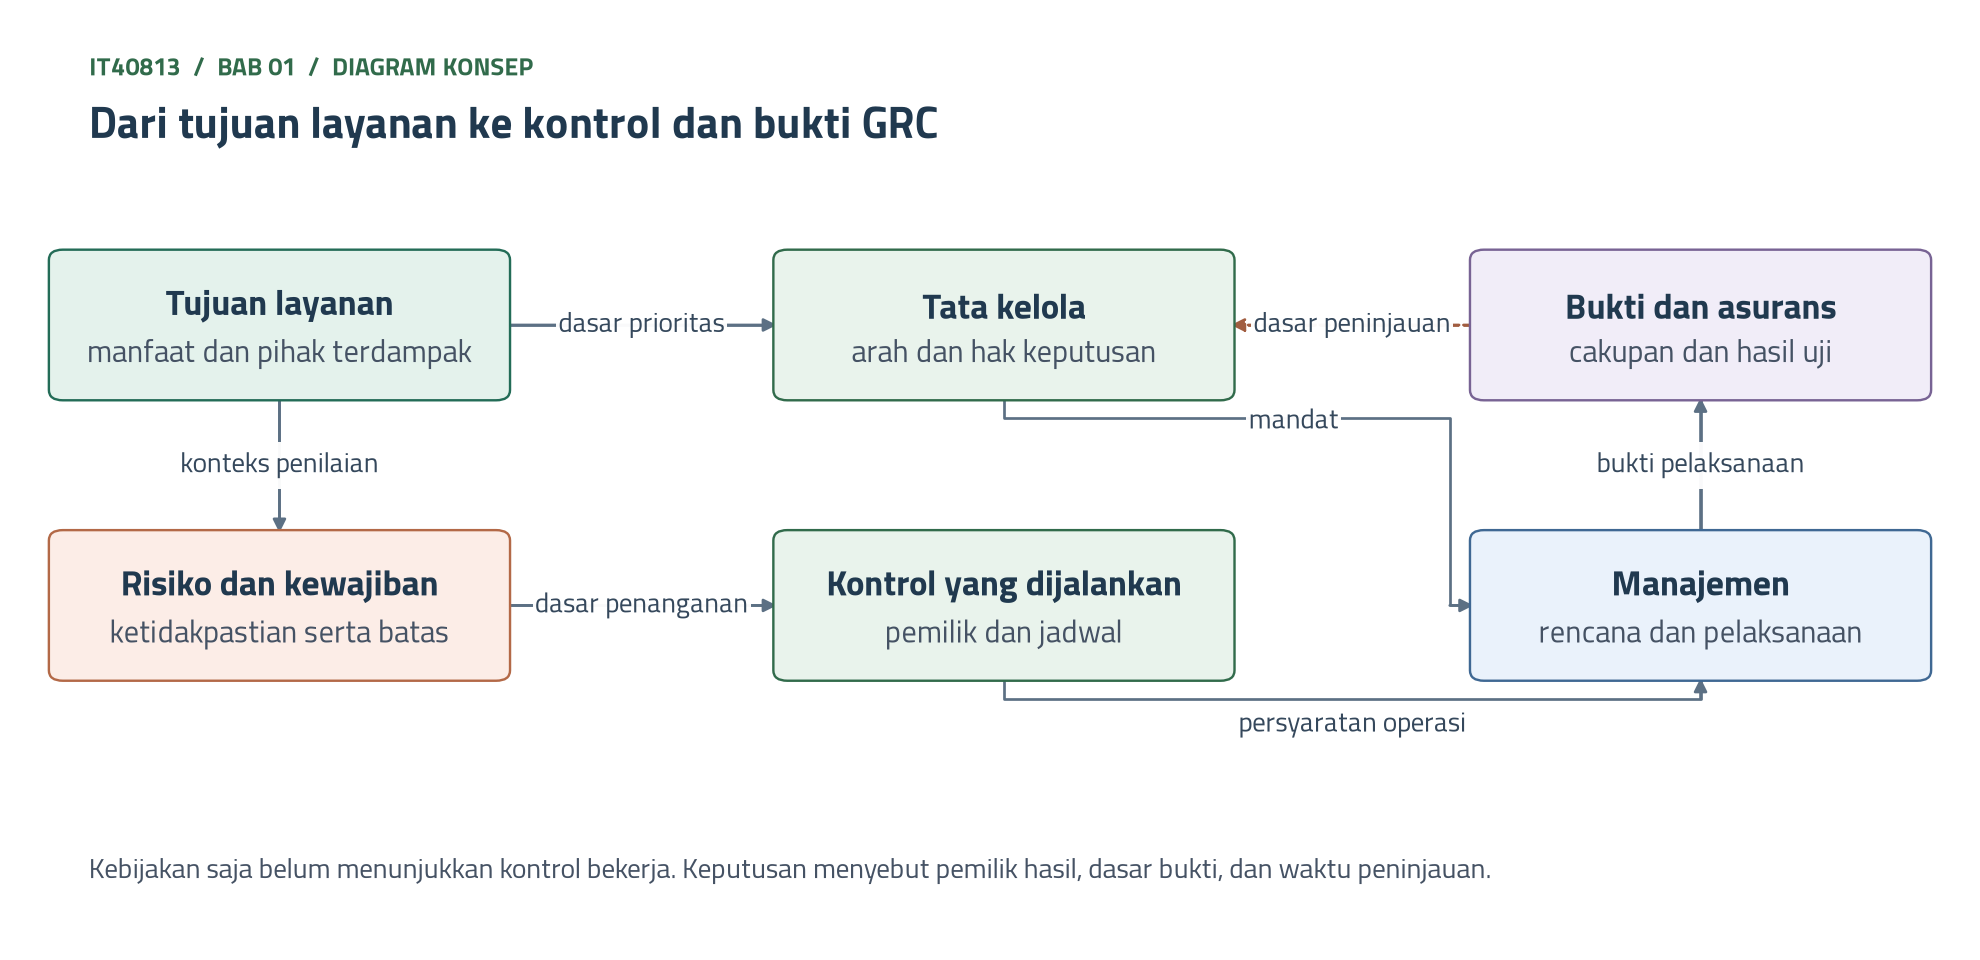
\includegraphics[width=\textwidth]{../figures/ch01-diagram-konsep.png}
  \caption{Dari tujuan layanan ke kontrol dan bukti GRC}
  \label{fig:ch01-ilustrasi-bab}
\end{figure}
}{}

Dua rujukan utama bab ini berasal dari International Organization for Standardization (ISO)
bersama International Electrotechnical Commission (IEC), serta dari ISACA. ISO/IEC
38500:2024 menjadi acuan arah dan pengawasan pemanfaatan TI. Control Objectives for
Information and Related Technologies (COBIT) 2019 membantu menghubungkan tujuan organisasi
dengan sistem tata kelola. Istilah GRC mengikuti Open Compliance and Ethics Group (OCEG)
serta Racz, Weippl, dan Seufert. Pembagian peran asurans mengikuti Three Lines Model dari
The Institute of Internal Auditors (IIA). Semua rujukan dipakai sebagai alat berpikir, lalu
diuji terhadap bukti pada kasus Medikara Health
\cite{iso38500-2024,cobit2019-intro,c01-oceg-grc,c01-racz2010,iia-tlm2026}.

\section{Mengapa Organisasi Membutuhkan Tata Kelola TI}

Tata kelola TI menetapkan arah, hak keputusan, dan cara meminta pertanggungjawaban atas
pemanfaatan TI. Weill dan Ross memandangnya sebagai penghubung antara keputusan TI dan
tujuan perusahaan, sekaligus pemantau kinerja dan akuntabilitas \cite{weill2004}. Masalah
teknis menjadi masalah tata kelola ketika pilihan tersebut memengaruhi manfaat, risiko,
sumber daya, atau hak pihak lain. Membeli aplikasi tidak menyelesaikan masalah bila
pemilik manfaat dan batas risikonya belum ditentukan.

Keputusan yang baik menyebut masalah layanan, alternatif, pihak terdampak, dasar
keputusan, serta waktu peninjauan. Satu pihak boleh mengusulkan pembelian dan pihak lain
menyetujuinya. Organisasi tetap membutuhkan pemilik hasil bisnis yang bertanggung jawab
setelah proyek selesai.

Analoginya seperti pengelola gedung. Pengelola tidak cukup membeli alarm kebakaran.
Pengelola menetapkan siapa memeriksa alarm, siapa memimpin evakuasi, dan bagaimana
penghuni mengetahui jalur keluar. Tata kelola TI memerlukan hubungan serupa antara tujuan,
pelaksana, dan pemeriksa.

Dua contoh penerapannya:
\begin{enumerate}
  \item Misalkan antrean pendaftaran pada 18 klinik turun dari 40 menjadi 25 menit
  setelah perubahan proses dan aplikasi. Direktur pelayanan menjadi pemilik hasil,
  sedangkan kepala TI bertanggung jawab pada kesiapan sistem. Bila waktu tunggu naik lagi
  dari 25 menit, direksi tahu siapa yang pertama diminta menjelaskan.
  \item Misalkan integrasi baru untuk Medikara+ menelan Rp450 juta per tahun. Dengan
  28.000 janji temu per bulan, atau 336.000 per tahun, biayanya sekitar Rp1.340 per janji
  temu. Keputusan menyetujuinya harus dibandingkan dengan nilai layanan serta biaya
  mempertahankan integrasi lama, bukan hanya harga implementasi.
\end{enumerate}

\subsection*{Tiga gejala yang memaksa organisasi bertanya}

Pertanyaan kemudian muncul: kapan kekosongan tata kelola mulai terasa? Umumnya lewat tiga
gejala, yaitu proyek gagal, data bocor, dan temuan audit.

Gejala pertama adalah proyek gagal. Flyvbjerg dan Budzier mempelajari 1.471 proyek TI.
Rata-rata pembengkakan biaya hanya 27 persen. Namun sekitar satu dari enam proyek masuk
kelompok ekstrem, dengan pembengkakan biaya rata-rata 200 persen dan keterlambatan jadwal
hampir 70 persen \cite{c01-flyvbjerg2011}. Misalkan Medikara menganggarkan Rp10 miliar untuk
modernisasi. Angka rata-rata berarti Rp12,7 miliar. Angka kelompok ekstrem berarti Rp30
miliar. Selisih sebesar itu bukan lagi urusan jadwal. Organisasi perlu tahu siapa yang
berhak menghentikan proyek dan pada batas apa.

Gejala kedua adalah data bocor. Laporan Verizon 2026 mencatat keterlibatan pihak ketiga
pada 48 persen pelanggaran data, naik dari 30 persen pada edisi sebelumnya
\cite{c01-verizon-dbir2026}. Laporan IBM 2026 mencatat rata-rata biaya pelanggaran data
global 4,99 juta dolar Amerika Serikat, dari 602 organisasi \cite{ibm-cdb2026}. Kedua angka
tidak boleh langsung dipindahkan ke Medikara, karena populasi dan cara hitungnya berbeda.
Laporan industri dipakai untuk mengajukan pertanyaan yang tepat, bukan untuk meramal
kerugian satu organisasi.

Gejala ketiga adalah temuan audit. Fakta dasar Medikara memuat temuan audit internal
tentang kontrol akses yang lemah. Misalkan audit memeriksa 30 dari 120 akun vendor dan
menemukan 6 akun masih aktif setelah penugasan berakhir, atau 20 persen sampel. Bila
sampel mewakili populasi, sekitar 24 akun bermasalah. Bila sampel dipilih tidak acak,
perkiraan itu gugur. Temuan baru bermakna ketika punya pemilik, tenggat, dan bukti
penutupan.

Tabel~\ref{tab:ch01-pemicu} merangkum empat pemicu GRC Medikara dan pertanyaan keputusan
yang menyertainya.
\begin{table}[!htb]
  \centering\small
  \caption{Pemicu GRC dan pertanyaan keputusan}\label{tab:ch01-pemicu}
  \begin{tabularx}{\textwidth}{|>{\raggedright\arraybackslash}p{0.27\textwidth}|>{\raggedright\arraybackslash}X|>{\raggedright\arraybackslash}X|}
    \hline
    \textbf{Pemicu} & \textbf{Pertanyaan organisasi} & \textbf{Bukti awal} \\ \hline
    Kebocoran vendor 2025 & Siapa membatasi akses vendor? & Kontrak dan daftar akun \\
    \hline
    Temuan kontrol akses & Siapa menutup temuan dan kapan? & Laporan audit \\ \hline
    Antrean panjang & Siapa memiliki hasil layanan? & Waktu tunggu agregat \\ \hline
    Biaya integrasi tinggi & Integrasi mana yang memberi nilai? & Biaya dan manfaat \\
    \hline
  \end{tabularx}
\end{table}

\begin{kasus}[title={Kasus Medikara Health: Insiden Vendor 2025 dalam Data Latihan}]
Fakta dasar kasus hanya menyebut kebocoran data pasien skala kecil lewat vendor pada 2025.
Mata kuliah IT40613 menambahkan data latihan berikut, dan bab ini memakai angka yang sama.
Misalkan kontrak pekerjaan vendor sudah selesai, tetapi akun dukungan vendor tetap aktif.
Selama 8 malam akun itu memanggil data kunjungan pada dua rumah sakit, 155 panggilan per
malam, sehingga 1.240 rekam kunjungan terbaca tanpa hubungan layanan dengan pekerjaan
vendor. Medikara baru mengetahuinya pada hari ke-11, lewat keluhan pasien.

Angka 1.240 setara sekitar 0,1 persen dari 1,2 juta kunjungan per tahun. Biaya langsung
latihan ini hanya Rp23,7 juta, belum termasuk sanksi, kehilangan kepercayaan, dan akibat
bagi pasien. Dua angka kecil itu tidak menjawab pertanyaan tata kelola. Siapa berwenang
mencabut akun ketika kontrak berakhir? Siapa memantau pemakaiannya? Siapa memutuskan
pemberitahuan kepada pasien? Bab 7 memakai data latihan ini dan menambahkan jamnya: hari
ke-1 Selasa pukul 20.00 WIB dan hari ke-11 Jumat pukul 20.00 WIB, lalu menghitung tenggat dari
kronologi itu.
\end{kasus}

\section{Tata Kelola dan Manajemen}

Pertanyaan berikutnya: siapa menetapkan arah, dan siapa menjalankannya? Tata kelola menilai
pilihan, memberi arah, dan memantau hasil. Manajemen menerjemahkan
arah menjadi rencana, pelaksanaan, serta pengendalian operasi. Keduanya bekerja berulang:
manajemen membawa bukti dan masalah baru, lalu pihak berwenang meninjau keputusan bila
konteks berubah.

COBIT 2019 memisahkan keduanya secara tegas. Tata kelola bekerja lewat \textit{Evaluate,
Direct, and Monitor}. Manajemen bekerja lewat \textit{Plan, Build, Run, and Monitor}, sesuai
arah dari badan pengarah. Dari 40 objektif dalam lima domain, satu domain berisi tata
kelola dan empat domain berisi manajemen \cite{cobit2019-intro}. ISO/IEC 38500:2024 memakai
tiga tugas yang sama untuk badan pengarah \cite{iso38500-2024}. Bab 2 dan Bab 4 membahas
rinciannya. Gambar~\ref{fig:ch01-tata-kelola-manajemen} memperlihatkan pembagian dan arus
informasi di antara keduanya.

\begin{figure}[!htb]
  \centering
  \begin{tikzpicture}[
  pita/.style={draw,rounded corners,fill=praditagreen!15,minimum width=11.4cm,
    minimum height=1.95cm},
  pita2/.style={pita,fill=orange!12},
  judul/.style={font=\scriptsize\bfseries,anchor=north west},
  tahap/.style={draw,rounded corners,align=center,minimum height=0.85cm,
    font=\scriptsize,fill=blue!8},
  panah/.style={-{Stealth[length=2mm]},thick}
]
  \node[pita] (atas) at (5.7,3.55) {};
  \node[judul] at (atas.north west) {Tata kelola: badan pengarah};
  \node[tahap,text width=3cm] at (1.8,3.3)
    {\textit{Evaluate}\\{\tiny\mdseries menilai pilihan dan akibat}};
  \node[tahap,text width=3cm] at (5.7,3.3)
    {\textit{Direct}\\{\tiny\mdseries memberi arah dan batas}};
  \node[tahap,text width=3cm] at (9.6,3.3)
    {\textit{Monitor}\\{\tiny\mdseries memantau hasil dan kepatuhan}};

  \node[pita2] (bawah) at (5.7,0) {};
  \node[judul] at (bawah.north west) {Manajemen: pelaksana sesuai mandat};
  \node[tahap,text width=2.2cm] at (1.35,-0.25)
    {\textit{Plan}\\{\tiny\mdseries merencanakan}};
  \node[tahap,text width=2.2cm] at (4.25,-0.25)
    {\textit{Build}\\{\tiny\mdseries membangun}};
  \node[tahap,text width=2.2cm] at (7.15,-0.25)
    {\textit{Run}\\{\tiny\mdseries menjalankan}};
  \node[tahap,text width=2.2cm] at (10.05,-0.25)
    {\textit{Monitor}\\{\tiny\mdseries memantau operasi}};

  \draw[panah] (3.1,2.56) -- node[left,font=\scriptsize,align=right]
    {mandat, prioritas,\\dan batas} (3.1,1);
  \draw[panah] (8.3,1) -- node[right,font=\scriptsize,align=left]
    {bukti pelaksanaan\\dan masalah baru} (8.3,2.56);
\end{tikzpicture}

  \caption{Pembagian tugas dan arus informasi antara tata kelola dan manajemen}
  \label{fig:ch01-tata-kelola-manajemen}
\end{figure}

Analoginya seperti pemilik restoran dan manajer dapur. Pemilik menentukan jenis layanan,
batas harga, dan standar kebersihan. Manajer dapur menyusun giliran kerja dan memeriksa
bahan setiap pagi. Pemilik tetap meminta laporan mutu, tetapi tidak perlu memilih urutan
memasak setiap pesanan.

Dua contoh penerapannya:
\begin{enumerate}
  \item Misalkan direksi menyetujui modernisasi lima rumah sakit dengan syarat layanan
  tetap berjalan. Manajemen menyusun jadwal migrasi bertahap dan prosedur pemulihan.
  Syarat itu keputusan tata kelola. Urutan kelima rumah sakit adalah keputusan manajemen.
  \item Misalkan komite hanya menerima laporan 90 persen pekerjaan selesai. Tanpa
  menilai manfaat dan risiko yang tersisa, komite belum memiliki dasar untuk mengizinkan
  peluncuran. Sisa 10 persen bisa saja berisi pekerjaan yang paling menentukan.
\end{enumerate}

Tabel~\ref{tab:ch01-peran} merangkum pembagian arah dan pelaksanaan pada tiga keputusan
Medikara.
\begin{table}[!htb]
  \centering\small
  \caption{Pembagian arah dan pelaksanaan}\label{tab:ch01-peran}
  \begin{tabularx}{\textwidth}{|>{\raggedright\arraybackslash}p{0.27\textwidth}|>{\raggedright\arraybackslash}X|>{\raggedright\arraybackslash}X|}
    \hline
    \textbf{Keputusan} & \textbf{Tata kelola} & \textbf{Manajemen} \\ \hline
    Identitas pasien tunggal & Tetapkan tujuan dan pemilik manfaat & Susun rencana
    integrasi \\ \hline
    Akses vendor & Tetapkan batas dan penanggung jawab & Berikan dan cabut akun \\
    \hline
    Investasi layanan & Pilih prioritas dan batas biaya & Kelola kontrak dan jadwal \\
    \hline
  \end{tabularx}
\end{table}

\subsection*{Jabatan bukan penentu}

Dua hal sering tertukar: jabatan penanda tangan dan jenis keputusan. Pembagiannya begini.
Memberi persetujuan atas batas investasi berbeda dari menyetujui jadwal pemasangan server.
Keputusan pertama mengalokasikan sumber daya dan menerima konsekuensi organisasi. Keputusan
kedua menjalankan rencana dalam kewenangan yang sudah diberikan. Seorang direktur yang
menandatangani jadwal sedang menjalankan manajemen. Seorang kepala TI yang ikut memilih
prioritas investasi di komite sedang ikut dalam tata kelola.

Pembedaan ini punya dua konsekuensi. Pertama, batas eskalasi harus tertulis. Misalkan
direksi menyetujui integrasi Rp450 juta per tahun dengan toleransi 10 persen, sehingga batas
atasnya Rp495 juta. Kenaikan menjadi Rp480 juta masih dalam kewenangan manajemen. Kenaikan
menjadi Rp540 juta, atau 20 persen, kembali ke direksi. Kedua, isi laporan ke direksi
berubah. Laporan tidak perlu memuat jadwal pemasangan di 18 klinik satu per satu. Laporan
memuat manfaat, risiko sisa, dan pilihan yang menunggu keputusan.

\section{Istilah Dasar GRC}

Keputusan dan pelaksanaan memerlukan bahasa yang sama. Apa beda risiko, kontrol, kepatuhan,
dan asurans? ISO 31000:2018 mendefinisikan risiko sebagai efek ketidakpastian terhadap tujuan, dan
kontrol sebagai tindakan yang mempertahankan atau mengubah risiko \cite{iso31000-2018}.
Kepatuhan adalah pemenuhan kewajiban yang berlaku, baik dari hukum, kontrak, maupun
komitmen yang dipilih organisasi. Asurans, menurut IIA, adalah pernyataan yang dimaksudkan
untuk meningkatkan keyakinan pemangku kepentingan atas proses tata kelola, manajemen
risiko, kepatuhan, dan kontrol \cite{iia-tlm2026}. Keyakinan itu lahir dari penilaian
berbasis bukti. Keempat istilah terhubung, tetapi menjawab pertanyaan berbeda.

Analoginya seperti aturan kas kecil. Aturan menetapkan batas pengeluaran, bukti kuitansi,
dan pihak yang menyetujui. Kuitansi menunjukkan transaksi terjadi. Pemeriksaan silang
terhadap buku kas memberi keyakinan bahwa aturan benar-benar dijalankan.

Dua contoh penerapannya:
\begin{enumerate}
  \item Misalkan risiko R-01 adalah akses vendor yang berlebihan menyebabkan
  pengungkapan data pasien. Kontrol AC-01 berupa peninjauan akses berkala menguji apakah
  hak akses masih diperlukan. Kode R-01 dan AC-01 tetap dipakai sampai Bab 14.
  \item Misalkan seluruh karyawan yang berjumlah sekitar 4.800 orang sudah menandatangani
  kebijakan akses, tetapi 6 dari 30 akun vendor yang diperiksa belum dicabut setelah
  penugasan berakhir. Kepatuhan administratif belum membuktikan efektivitas pencabutan
  akses.
\end{enumerate}

Tabel~\ref{tab:ch01-istilah} merangkum istilah GRC dan bukti penerapannya.
\begin{table}[!htb]
  \centering\small
  \caption{Istilah GRC dan bukti penerapannya}\label{tab:ch01-istilah}
  \begin{tabularx}{\textwidth}{|>{\raggedright\arraybackslash}p{0.22\textwidth}|>{\raggedright\arraybackslash}X|>{\raggedright\arraybackslash}X|}
    \hline
    \textbf{Istilah} & \textbf{Pertanyaan} & \textbf{Contoh bukti} \\ \hline
    Tata kelola & Siapa memutuskan arah dan batas? & Notulen dan delegasi \\ \hline
    Manajemen & Bagaimana arah dijalankan? & Rencana dan laporan kerja \\ \hline
    Risiko & Apa yang mengancam tujuan? & Skenario R-01 \\ \hline
    Kontrol & Apa yang mengubah risiko? & Hasil peninjauan AC-01 \\ \hline
    Kepatuhan & Kewajiban mana yang dipenuhi? & Register kewajiban \\ \hline
    Asurans & Mengapa hasil layak dipercaya? & Kertas kerja pengujian \\ \hline
  \end{tabularx}
\end{table}

\begin{kasus}[title={Kasus Medikara Health: Dari Insiden ke Pemilik Keputusan}]
Kebocoran data skala kecil melalui vendor pada 2025 adalah fakta kasus. Misalkan tim
menelusuri insiden itu ke akun dukungan yang masih aktif setelah kontrak pekerjaan
selesai. Tim mencatat R-01, menetapkan pemilik risiko pada fungsi bisnis yang menentukan
pemrosesan, dan mengusulkan AC-01. Bukti yang diminta adalah daftar akun, dasar
pemberian akses, hasil peninjauan, serta tindakan pencabutan. Besar kecilnya insiden
tidak menghilangkan kebutuhan menilai kewajiban hukum. Pasal 46 Undang-Undang (UU) Nomor
27 Tahun 2022 tentang Pelindungan Data Pribadi (PDP) mengatur pemberitahuan tertulis paling
lambat $3 \times 24$ jam \cite{uu27-2022-pdp}. Bab 7 mengujinya dengan kronologi.
\end{kasus}

\subsection*{Kebijakan, standar, prosedur, dan pedoman}

Empat dokumen ini sering tertukar. Pembagiannya begini. Kebijakan menyatakan arah dan
batas. Standar organisasi menetapkan persyaratan minimum. Prosedur menjelaskan urutan
kerja. Pedoman membantu memilih cara yang sesuai, tanpa mengikat. Kata ``standar'' di sini
berarti aturan internal organisasi, berbeda dari standar internasional seperti ISO/IEC
27001. Tabel~\ref{tab:ch01-dokumen} memakai kontrol AC-01 sebagai contoh.

\begin{table}[!htb]
  \centering\small
  \caption{Dokumen dan catatan untuk kontrol AC-01 (angka pengandaian)}
  \label{tab:ch01-dokumen}
  \begin{tabularx}{\textwidth}{|>{\raggedright\arraybackslash}p{0.22\textwidth}|>{\raggedright\arraybackslash}X|}
    \hline
    \textbf{Jenis} & \textbf{Isi pada AC-01} \\ \hline
    Kebijakan & Akses vendor hanya berlaku selama penugasan \\ \hline
    Standar organisasi & Akun dicabut paling lambat 1 hari kerja setelah penugasan berakhir,
    dan ditinjau setiap bulan \\ \hline
    Prosedur & Pengelola vendor menarik daftar akun, pemilik layanan menandai akun yang
    masih perlu, admin mencabut sisanya \\ \hline
    Pedoman & Pakai akun per orang, bukan akun bersama, bila sistem memungkinkan \\ \hline
    Catatan sebagai bukti & Peninjauan bulan berikutnya: 120 akun ditinjau, 24 akun dicabut,
    tanggal dan penanggung jawab tercatat \\ \hline
  \end{tabularx}
\end{table}

Kebijakan tanpa prosedur dan bukti pelaksanaan belum menunjukkan bahwa kontrol bekerja.
Baris terakhir pada tabel itulah yang dibaca auditor.

\subsection*{Siapa memberi keyakinan?}

Pertanyaan kemudian muncul: siapa yang memeriksa, kalau pelaksana tidak boleh menilai
pekerjaannya sendiri? Three Lines Model dari IIA membedakan peran, bukan departemen.
Manajemen sebagai lini pertama memiliki dan mengelola risiko. Peran lini kedua memberi
keahlian, dukungan, pemantauan, dan tantangan. Audit internal sebagai lini ketiga memberi
asurans yang independen dan objektif. Badan pengarah memberi arah strategis dan pengawasan
\cite{iia-tlm2026}. Tabel~\ref{tab:ch01-tiga-lini} menerapkannya pada AC-01, dengan contoh
pemilik Sistem Informasi Manajemen Rumah Sakit (SIMRS). Bab 12 membahas model ini lebih dalam.

\begin{table}[!htb]
  \centering\small
  \caption{Three Lines Model pada kontrol AC-01}\label{tab:ch01-tiga-lini}
  \begin{tabularx}{\textwidth}{|>{\raggedright\arraybackslash}p{0.22\textwidth}|>{\raggedright\arraybackslash}X|>{\raggedright\arraybackslash}X|}
    \hline
    \textbf{Peran} & \textbf{Contoh pemilik} & \textbf{Tanggung jawab} \\ \hline
    Badan pengarah & Direksi dan dewan komisaris sesuai kewenangan & Menetapkan arah dan
    meminta laporan \\ \hline
    Lini pertama & Pemilik SIMRS dan layanan & Menjalankan kontrol AC-01 \\ \hline
    Lini kedua & Risiko, privasi, keamanan & Memantau dan menantang \\ \hline
    Lini ketiga & Audit internal & Menguji secara independen \\ \hline
  \end{tabularx}
\end{table}

Pembedaan ini berlaku juga untuk vendor. IIA menegaskan bahwa kegiatan yang dialihkan ke
penyedia luar tidak berubah perannya dalam model, dan akuntabilitas badan pengarah atas
kegiatan itu tidak berubah \cite{iia-tlm2026}. Medikara dapat menyerahkan pekerjaan kepada
vendor, tetapi tidak dapat menyerahkan pertanggungjawaban atas keputusannya.

\section{GRC sebagai Satu Kesatuan}

Bila tiap istilah menjawab pertanyaan berbeda, mengapa ketiganya disatukan dalam satu
singkatan? OCEG mendefinisikan GRC sebagai kumpulan kemampuan terpadu yang memungkinkan organisasi
mencapai tujuan secara andal, sekaligus menangani ketidakpastian dan bertindak dengan
integritas \cite{c01-oceg-grc}. Racz, Weippl, dan Seufert merumuskan GRC sebagai pendekatan
terpadu dan menyeluruh terhadap tata kelola, risiko, dan kepatuhan di seluruh organisasi.
Pendekatan itu memastikan organisasi bertindak etis dan sesuai dengan \textit{risk
appetite}, kebijakan internal, serta regulasi, lewat penyelarasan strategi, proses,
teknologi, dan orang \cite{c01-racz2010,c01-racz2011}. Kedua definisi menyimpulkan hal yang
sama: GRC bukan tiga unit yang terpisah, dan bukan satu produk perangkat lunak.

Analoginya seperti pasien yang berobat ke tiga dokter tanpa rekam medis bersama. Tiap
dokter meminta pemeriksaan darah sendiri, memberi resep sendiri, dan tidak tahu obat dari
dokter lain. Setiap dokter bekerja benar menurut catatannya, tetapi pasien menanggung
biaya berlipat dan risiko obat yang saling berbenturan.

Dua contoh penerapannya:
\begin{enumerate}
  \item Misalkan audit internal, bagian kepatuhan, dan keamanan informasi masing-masing
  meminta daftar akun kepada 5 rumah sakit dan 18 klinik setiap triwulan. Jumlahnya $3
  \times 23 \times 4 = 276$ permintaan per tahun untuk bukti yang sama. Dengan satu
  register dan satu jadwal, permintaan turun menjadi $23 \times 4 = 92$. Bila satu
  permintaan memakan 2 jam kerja, fasilitas menghemat $184 \times 2 = 368$ jam per tahun.
  \item Misalkan kontrol AC-01 mendukung tiga acuan sekaligus: UU 27/2022 Pasal 35, 36, 37, dan
  39, dengan Pasal 39 sebagai acuan utama, ISO/IEC 27001:2022 Annex A 5.18, dan National
  Institute of Standards and Technology
  Cybersecurity Framework (NIST CSF) 2.0 PR.AA-05. Tanpa register bersama, satu kontrol
  tercatat tiga kali dengan tiga nama. Pemetaan ini menunjukkan kontribusi, bukan
  kesetaraan, sehingga tiap acuan tetap diperiksa pada Bab 14.
\end{enumerate}

Gambar~\ref{fig:ch01-grc-terpadu} memperlihatkan bentuk kerja terpadu. Ketiga fungsi berangkat
dari tujuan layanan yang sama dan mencatat hasilnya pada satu register.
Tabel~\ref{tab:ch01-terpadu} membandingkannya dengan cara kerja terpisah.

\begin{figure}[!htb]
  \centering
  \begin{tikzpicture}[
  kotak/.style={draw,rounded corners,align=center,minimum height=1cm,
    font=\scriptsize,fill=blue!8},
  panah/.style={-{Stealth[length=2mm]},thick}
]
  \node[kotak,fill=praditagreen!15,text width=10.4cm,minimum height=0.8cm] (tujuan)
    at (5.4,4.5) {\textbf{Tujuan layanan}: manfaat dan pihak terdampak};

  \node[kotak,text width=3cm] (g) at (1.8,2.85)
    {\textbf{Tata kelola}\\{\tiny\mdseries arah dan hak keputusan}};
  \node[kotak,text width=3cm] (r) at (5.4,2.85)
    {\textbf{Risiko}\\{\tiny\mdseries ketidakpastian serta batas}};
  \node[kotak,text width=3cm] (c) at (9,2.85)
    {\textbf{Kepatuhan}\\{\tiny\mdseries kewajiban yang berlaku}};

  \node[kotak,fill=orange!12,text width=10.4cm] (reg) at (5.4,1.2)
    {\textbf{Satu register bersama}\\
     {\tiny\mdseries ID tetap: pemicu P-01, risiko R-01, kontrol AC-01, kewajiban,
     bukti, dan pemilik}};

  \node[kotak,fill=green!10,text width=10.4cm,minimum height=0.8cm] (bukti) at (5.4,-0.4)
    {\textbf{Bukti dan asurans}: cakupan dan hasil uji};

  \draw[panah] (g.north |- tujuan.south) -- (g.north);
  \draw[panah] (r.north |- tujuan.south) -- (r.north);
  \draw[panah] (c.north |- tujuan.south) -- (c.north);
  \draw[panah] (g.south) -- (g.south |- reg.north);
  \draw[panah] (r.south) -- (r.south |- reg.north);
  \draw[panah] (c.south) -- (c.south |- reg.north);
  \draw[panah] (reg) -- (bukti);
  \draw[panah,dashed] (bukti.east) -- ++(0.45,0) |- (tujuan.east);
  \node[font=\tiny,rotate=90,fill=white,inner sep=1pt] at (11.05,2.05)
    {dasar peninjauan};
\end{tikzpicture}

  \caption{GRC terpadu: tiga fungsi berbagi satu tujuan, satu register, dan satu dasar peninjauan}
  \label{fig:ch01-grc-terpadu}
\end{figure}

\begin{table}[!htb]
  \centering\small
  \caption{Cara kerja terpisah dan terpadu}\label{tab:ch01-terpadu}
  \begin{tabularx}{\textwidth}{|>{\raggedright\arraybackslash}p{0.22\textwidth}|>{\raggedright\arraybackslash}X|>{\raggedright\arraybackslash}X|}
    \hline
    \textbf{Aspek} & \textbf{Terpisah} & \textbf{Terpadu} \\ \hline
    Pengenal & Tiap unit punya nama sendiri & ID tetap: R-01, AC-01 \\ \hline
    Permintaan bukti & 276 permintaan per tahun & 92 permintaan per tahun \\ \hline
    Laporan ke direksi & Tiga laporan, tiga skala & Satu gambaran, sumber dapat ditelusuri \\
    \hline
    Peninjauan & Menurut jadwal tiap unit & Menurut tujuan layanan dan pemicu \\ \hline
  \end{tabularx}
\end{table}

Alur yang sama tampak pada Gambar~\ref{fig:ch01-ilustrasi-bab}. Tujuan layanan memberi dasar
prioritas bagi tata kelola, dan konteks penilaian bagi risiko dan kewajiban. Tata kelola
memberi mandat kepada manajemen. Risiko dan kewajiban menjadi dasar penanganan, yang
diwujudkan dalam kontrol yang dijalankan. Kontrol menjadi persyaratan operasi bagi
manajemen. Manajemen menghasilkan bukti pelaksanaan, yang dinilai dalam bukti dan asurans.
Hasilnya menjadi dasar peninjauan bagi tata kelola, dan siklus berulang.

\subsection*{Terpadu tidak berarti dilebur}

Dua hal pada GRC sering tertukar: terpadu dan dilebur. Pembagiannya begini. Terpadu berarti
memakai tujuan, pengenal, dan bukti yang sama. Dilebur berarti satu unit mengerjakan semua
peran. Peleburan justru merusak asurans, karena pelaksana menilai pekerjaannya sendiri. IIA
menempatkan independensi sebagai dasar asurans yang dapat dipercaya, sekaligus mengingatkan
bahwa independensi tidak boleh ditafsirkan sebagai isolasi \cite{iia-tlm2026}.

Keputusan memakai satu register punya dua konsekuensi. Pertama, register memerlukan pemilik
dan aturan perubahan, karena satu kesalahan kini terbaca oleh semua unit. Kedua, organisasi
menanggung biaya menyamakan istilah di awal. Misalkan menyamakan 40 baris risiko memakan
20 jam kerja. Biaya itu sebanding bila menghemat 368 jam per tahun seperti pada contoh di
atas, tetapi belum tentu sebanding bagi organisasi yang hanya punya satu lokasi. Bab 14
membahas alat GRC, setelah cara kerjanya jelas.

\section{Peta Kerangka dan Regulasi}

Rujukan mana yang dipakai untuk pertanyaan tertentu? Kerangka menyediakan cara
mengelompokkan masalah. Standar menyediakan prinsip, panduan,
atau persyaratan sesuai jenisnya. Regulasi menetapkan kewajiban hukum dalam ruang lingkup
tertentu. Organisasi memilih kerangka berdasarkan pertanyaan yang perlu dijawab, lalu
menelusuri kewajiban ke sumber hukum aslinya.

Analoginya seperti peta jalan, aturan lalu lintas, dan buku servis kendaraan. Peta membantu
memilih rute. Aturan mengikat pengguna jalan. Buku servis membantu merawat kendaraan.
Ketiganya dapat dipakai dalam satu perjalanan tanpa saling menggantikan.

Dua contoh penerapannya:
\begin{enumerate}
  \item Misalkan Medikara perlu menetapkan siapa menerima risiko layanan. ISO/IEC 38500
  dan COBIT membantu merancang hak keputusan. Daftar konfigurasi server tidak menjawab
  pertanyaan tersebut. Medikara juga tidak perlu menjalankan semuanya sekaligus: bila 52
  staf TI menanggung 40 objektif COBIT, satu objektif hanya kebagian 1,3 orang. Karena itu
  Bab 4 memilih objektif prioritas.
  \item Misalkan tim perlu menentukan masa simpan rekam medis. Tim membaca peraturan
  sektor kesehatan terlebih dahulu, lalu mencari kontrol dan arsitektur yang
  mendukungnya. Urutan terbalik membuat 5 rumah sakit membangun fitur untuk kewajiban yang
  belum dibaca.
\end{enumerate}

Tabel~\ref{tab:ch01-kerangka} merupakan peta belajar, bukan daftar yang harus diterapkan
seluruhnya. Nama standar dicantumkan bersama versinya agar keputusan dapat ditelusuri ketika
rujukan berubah. Tabel itu memakai beberapa singkatan: Information Technology Infrastructure
Library (ITIL), Peraturan Menteri Kesehatan (Permenkes), Peraturan Pemerintah (PP), Committee
of Sponsoring Organizations of the Treadway Commission (COSO), \textit{Enterprise Risk
Management} (ERM), dan \textit{Artificial Intelligence} (AI).

\begin{table}[!htb]
  \centering\small
  \caption{Peta pertanyaan dan rujukan semester}\label{tab:ch01-kerangka}
  \begin{tabularx}{\textwidth}{|>{\raggedright\arraybackslash}p{0.27\textwidth}|>{\raggedright\arraybackslash}X|>{\raggedright\arraybackslash}p{0.17\textwidth}|>{\raggedright\arraybackslash}p{0.08\textwidth}|}
    \hline
    \textbf{Pertanyaan} & \textbf{Rujukan} & \textbf{Jenis} & \textbf{Bab} \\ \hline
    Siapa memberi arah dan memutuskan? & ISO/IEC 38500:2024 \cite{iso38500-2024} & Prinsip &
    2, 8 \\ \hline
    Bagaimana sistem tata kelola disusun? & COBIT 2019 \cite{cobit2019-intro}, ITIL
    \cite{itil4} & Kerangka & 4, 8 \\ \hline
    Aturan mana yang mengikat? & UU 27/2022 \cite{uu27-2022-pdp}, Permenkes 24/2022
    \cite{permenkes24-2022}, PP 71/2019 \cite{pp71-2019-pste} & Hukum & 3, 7 \\ \hline
    Ketidakpastian mana yang mengancam tujuan? & ISO 31000:2018 \cite{iso31000-2018}, COSO ERM
    2017 \cite{cosoerm2017} & Panduan & 5 \\ \hline
    Apakah informasi dan vendor aman? & ISO/IEC 27001:2022 \cite{iso27001-2022}, NIST CSF 2.0
    \cite{nistcsf2} & Persyaratan, kerangka & 6, 9 \\ \hline
    Apakah layanan bertahan saat gangguan? & ISO 22301:2019 \cite{iso22301-2019} & Persyaratan
    & 10 \\ \hline
    Bagaimana AI dikendalikan? & ISO/IEC 42001:2023 \cite{iso42001-2023} & Persyaratan & 11
    \\ \hline
    Mengapa hasil layak dipercaya? & Global Internal Audit Standards \cite{iia-gias2024},
    Three Lines Model \cite{iia-tlm2026} & Standar profesi, model peran & 12, 13, 14 \\ \hline
  \end{tabularx}
\end{table}

\subsection*{Patuh dan bersertifikat}

Dua hal sering tertukar: mematuhi hukum dan memegang sertifikat. Pembagiannya begini.
Regulasi berlaku karena organisasi masuk ruang lingkupnya, tanpa perlu memilih. Standar
seperti ISO/IEC 27001 dipilih organisasi, atau diminta oleh mitra lewat kontrak. Sertifikat
menunjukkan sistem manajemen memenuhi persyaratan untuk ruang lingkup tertentu. Sertifikat
tidak membuktikan pemenuhan seluruh kewajiban UU PDP. Sebaliknya, memenuhi satu pasal hukum
juga belum berarti risikonya terkendali, dan Latihan 2 menguji hal ini.

Versi rujukan perlu diperiksa ulang. Per 30 Oktober 2026, informasi produk ISACA telah
menyebut COBIT 7, sementara halaman kerangka resminya masih menyediakan publikasi COBIT
2019. PeopleCert menerbitkan ITIL (Version 5) pada 2026. ISO 31000 dan ISO 22301 sedang
direvisi. Modul ini memakai versi yang tertulis pada tabel. Tim mencatat versi yang dipakai
dan tanggal pemeriksaannya, bukan menebak isi versi berikutnya.

\section{Capstone Bersama dan Kasus Medikara Health}

Di mana semua konsep itu diterapkan? Capstone menghasilkan satu Cetak Biru Transformasi
Digital yang dipelihara bersama empat
mata kuliah. IT40513 menyusun arsitektur \textit{enterprise}, IT40613 menyusun platform dan
\textit{Application Programming Interface} (API), IT40713 merancang layanan serta
infrastruktur \textit{cloud}, dan IT40813 menetapkan tata kelola, risiko, serta kepatuhan.
Artefak harus menggunakan nama layanan, sistem, data, dan angka biaya yang sama.
Gambar~\ref{fig:ch01-capstone} memperlihatkan hubungan keempat mata kuliah dengan tonggak C1
sampai C4.

\begin{figure}[!htb]
  \centering
  \begin{tikzpicture}[
  matkul/.style={draw,rounded corners,align=center,text width=2.5cm,
    minimum height=1.25cm,font=\scriptsize,fill=blue!8},
  tonggak/.style={draw,rounded corners,align=center,text width=2.5cm,
    minimum height=1.25cm,font=\scriptsize,fill=praditagreen!15},
  panah/.style={-{Stealth[length=2mm]},thick}
]
  \node[matkul] (ea) at (0,3.3)
    {IT40513\\{\tiny\mdseries arsitektur \textit{enterprise}}};
  \node[matkul] (api) at (3.1,3.3)
    {IT40613\\{\tiny\mdseries platform dan API}};
  \node[matkul] (cloud) at (6.2,3.3)
    {IT40713\\{\tiny\mdseries layanan dan \textit{cloud}}};
  \node[matkul,fill=orange!12] (grc) at (9.3,3.3)
    {IT40813\\{\tiny\mdseries tata kelola, risiko,}\\{\tiny\mdseries dan kepatuhan}};

  \node[draw,rounded corners,align=center,fill=green!10,text width=11.4cm,
    minimum height=0.95cm,font=\scriptsize] (cetak) at (4.65,1.55)
    {\textbf{Cetak Biru Transformasi Digital}\\
     {\tiny\mdseries satu organisasi; nama layanan, sistem, data, dan biaya yang sama}};

  \foreach \sumber in {ea,api,cloud,grc}
    \draw[panah] (\sumber.south) -- (\sumber.south |- cetak.north);

  \node[tonggak] (c1) at (0,0)
    {\textbf{C1} Konteks dan Strategi\\{\tiny\mdseries Pertemuan 1 sampai 3}};
  \node[tonggak] (c2) at (3.1,0)
    {\textbf{C2} Kondisi Saat Ini\\{\tiny\mdseries Pertemuan 4 sampai 7}};
  \node[tonggak] (c3) at (6.2,0)
    {\textbf{C3} Kondisi Target\\{\tiny\mdseries Pertemuan 8 sampai 11}};
  \node[tonggak] (c4) at (9.3,0)
    {\textbf{C4} Peta Jalan dan Tata Kelola\\{\tiny\mdseries Pertemuan 12 sampai 14}};

  \draw[panah] (c1) -- (c2);
  \draw[panah] (c2) -- (c3);
  \draw[panah] (c3) -- (c4);
  \foreach \tonggak in {c1,c2,c3,c4}
    \draw[panah] (\tonggak.north |- cetak.south) -- (\tonggak.north);
\end{tikzpicture}

  \caption{Empat mata kuliah mengisi satu cetak biru lewat empat tonggak}
  \label{fig:ch01-capstone}
\end{figure}

Analoginya seperti satu rancangan gedung. Gedung memerlukan gambar arsitektur, struktur,
listrik, dan jalur evakuasi yang memakai ukuran sama. Empat gambar yang bagus tetapi berbeda
letak pintunya tidak membentuk rancangan yang dapat dibangun.

Dua contoh penerapannya:
\begin{enumerate}
  \item Misalkan IT40613 membuka API hasil laboratorium dari 1 laboratorium rujukan ke 18
  klinik. GRC harus menilai penerima data, tujuan akses, dan kontrolnya sebelum arsitektur
  target disepakati.
  \item Misalkan IT40713 memindahkan Medikara+, dengan 28.000 janji temu per bulan, ke
  \textit{cloud}. GRC meninjau tanggung jawab vendor dan persyaratan lokasi data, lalu
  mengembalikan batasan kepada tim arsitektur.
\end{enumerate}

Tabel~\ref{tab:ch01-capstone} merangkum tonggak dan kontribusi GRC. Perubahan pada satu
tonggak bisa kembali ke tonggak sebelumnya. Bila arsitektur berubah pada C3, daftar risiko
dari C2 ikut ditinjau.

\begin{table}[!htb]
  \centering\small
  \caption{Tonggak dan kontribusi GRC}\label{tab:ch01-capstone}
  \begin{tabularx}{\textwidth}{|>{\raggedright\arraybackslash}p{0.3\textwidth}|>{\raggedright\arraybackslash}p{0.16\textwidth}|>{\raggedright\arraybackslash}X|}
    \hline
    \textbf{Tonggak} & \textbf{Pertemuan} & \textbf{Luaran utama} \\ \hline
    C1 Konteks dan Strategi & 1 sampai 3 & Profil, hak keputusan, kewajiban \\ \hline
    C2 Kondisi Saat Ini & 4 sampai 7 & Kapabilitas, risiko, celah keamanan dan privasi \\
    \hline
    C3 Kondisi Target & 8 sampai 11 & Tata kelola target, vendor, kelangsungan, AI \\
    \hline
    C4 Peta Jalan dan Tata Kelola & 12 sampai 14 & Asurans, indikator, peta jalan \\
    \hline
  \end{tabularx}
\end{table}

\begin{kasus}[title={Kasus Medikara Health: Profil yang Dipakai Bersama}]
PT Medikara Nusa Sehat (``Medikara Health'') adalah organisasi fiktif, jaringan layanan
kesehatan swasta dengan 5 rumah sakit (Jakarta, Bekasi, Depok, Bogor, Bandung), 18 klinik
pratama, 1 laboratorium rujukan, dan 12 apotek. Sekitar 4.800 karyawan melayani sekitar 1,2
juta kunjungan pasien per tahun. Mata kuliah lain menambahkan rincian sekitar 640 dokter, 52
staf TI dengan tim platform 6 orang, dan 28.000 janji temu per bulan lewat Medikara+.

SIMRS berjalan \textit{on-premise} di tiap rumah sakit dengan versi berbeda karena hasil
akuisisi. \textit{Enterprise Resource Planning} (ERP)
keuangan sudah terpusat. Medikara+ dibuat oleh vendor. Integrasi ke Badan Penyelenggara
Jaminan Sosial (BPJS) Kesehatan dan SATUSEHAT berbentuk \textit{point-to-point}. Data pasien
tersebar, dan banyak laporan manajemen masih disusun dengan \textit{spreadsheet}.

Strategi 2026 sampai 2030 bernama ``Satu Pasien, Satu Rekam Medis''. Pemicunya ada empat:
insiden kebocoran vendor pada 2025, temuan audit internal tentang kontrol akses, antrean
layanan yang panjang, dan biaya integrasi yang tinggi. Fakta dasar ini tetap. Rincian
tambahan dalam bab ini ditandai ``Misalkan'' atau ``data latihan''.
\end{kasus}

\section{Pemangku Kepentingan dan Pemicu GRC}

Setelah organisasi dipilih, siapa saja yang harus diperhitungkan? Freeman mendefinisikan
pemangku kepentingan sebagai kelompok atau individu yang dapat
memengaruhi, atau terpengaruh oleh, pencapaian tujuan organisasi \cite{c01-freeman2010}.
Definisi itu memuat dua arah, yaitu pengaruh dan dampak. Peta pemangku kepentingan menampilkan
keduanya, lalu menunjukkan siapa berkepentingan, siapa memutuskan, dan siapa terdampak. Pemicu
GRC adalah peristiwa atau keadaan yang memaksa organisasi mengambil keputusan, misalnya
insiden, temuan audit, atau aturan baru.

Analoginya seperti rapat RT yang memutuskan jam penutupan portal. Ketua dan pengurus hadir,
lalu keputusan diambil dengan sah. Warga di ujung gang yang pulang malam tidak hadir, padahal
merekalah yang paling terdampak. Keputusan yang sah belum tentu sudah mendengar pihak yang
menanggung akibatnya.

Dua contoh dari Medikara Health:
\begin{enumerate}
  \item Pada insiden vendor, data latihan mencatat 1.240 rekam kunjungan terbaca. Pasien
  menanggung dampak tinggi, tetapi tidak hadir di rapat. Bila rapat hanya melihat biaya
  langsung Rp23,7 juta, insiden tampak selesai. Bila kepentingan pasien diwakili, pertanyaan
  berpindah ke pemberitahuan dan pemulihan kepercayaan.
  \item Pada pemicu antrean, misalkan 720.000 dari 1,2 juta kunjungan terjadi di 18 klinik.
  Penurunan antrean 15 menit berarti $720.000 \times 15 \div 60 = 180.000$ jam waktu tunggu
  pasien per tahun. Angka sebesar ini tidak muncul bila laporan hanya menghitung biaya TI.
\end{enumerate}

Gambar~\ref{fig:ch01-peta-pemangku} memetakan delapan pemangku kepentingan Medikara untuk
pemicu insiden vendor. Skala 1 sampai 3 adalah penilaian tim, bukan pengukuran. Sel oranye
menandai pihak yang berdampak tinggi tetapi berpengaruh rendah, sehingga perlu wakil yang
jelas.

\begin{figure}[!htb]
  \centering
  \begin{tikzpicture}[
  sel/.style={draw,align=center,text width=2.95cm,minimum height=1.2cm,
    font=\scriptsize,fill=blue!8,inner sep=2pt},
  kosong/.style={sel,fill=white},
  panah/.style={-{Stealth[length=2mm]},thick}
]
  % Baris atas: dampak tinggi. Kolom kanan: pengaruh tinggi.
  \node[sel,fill=orange!12] at (0,2.5)
    {S-01 Pasien\\{\tiny\mdseries wakili suaranya}};
  \node[sel] at (3.15,2.5)
    {S-04 Klinisi\\S-05 Manajemen TI\\{\tiny\mdseries libatkan dalam rancangan}};
  \node[sel,fill=praditagreen!15] at (6.3,2.5)
    {S-02 Direksi\\{\tiny\mdseries memutuskan dan menerima risiko}};

  \node[kosong] at (0,1.25) {};
  \node[sel] at (3.15,1.25)
    {S-06 Vendor Medikara+\\S-07 Audit internal\\{\tiny\mdseries minta batas dan bukti}};
  \node[sel] at (6.3,1.25)
    {S-03 Dewan komisaris\\{\tiny\mdseries terima laporan pengawasan}};

  \node[kosong] at (0,0) {};
  \node[kosong] at (3.15,0) {};
  \node[sel] at (6.3,0)
    {S-08 Regulator sektor\\{\tiny\mdseries penuhi lewat saluran resmi}};

  \draw[panah] (-1.65,-0.75) -- (-1.65,3.25);
  \node[font=\scriptsize,rotate=90,anchor=south] at (-1.95,1.25)
    {Dampak bila pemicu diabaikan};
  \draw[panah] (-1.65,-0.75) -- (8,-0.75);
  \node[font=\scriptsize,anchor=north] at (3.15,-0.8)
    {Pengaruh pada keputusan};
  \node[font=\tiny,anchor=north] at (0,-0.8) {1 rendah};
  \node[font=\tiny,anchor=north] at (6.3,-0.8) {3 tinggi};
  \node[font=\tiny,anchor=east] at (-1.68,2.5) {3};
  \node[font=\tiny,anchor=east] at (-1.68,1.25) {2};
  \node[font=\tiny,anchor=east] at (-1.68,0) {1};
\end{tikzpicture}

  \caption{Peta pemangku kepentingan Medikara untuk pemicu insiden vendor (penilaian contoh)}
  \label{fig:ch01-peta-pemangku}
\end{figure}

Dua hal pada peta ini sering tertukar: pengaruh dan dampak. Pembagiannya begini. Pengaruh
adalah kemampuan mengubah keputusan. Dampak adalah besarnya akibat yang ditanggung bila pemicu
diabaikan. Regulator sektor berpengaruh tinggi, tetapi bukan pihak yang kehilangan
kerahasiaan. Pasien mengalami sebaliknya. Pemetaan ini punya dua konsekuensi. Pertama, tim
tidak boleh mengurutkan pihak hanya menurut jabatan. Kedua, sel kosong perlu dibaca. Sel
kiri bawah yang kosong wajar, tetapi sel kiri atas yang kosong patut dicurigai, karena tim
mungkin belum mencari pihak yang tidak hadir di rapat.

\subsection*{Menulis pemicu tanpa mencampur fakta dan dugaan}

Pemicu yang berguna menyebut tujuan terdampak, status informasi, sumber dengan tanggal, dan
keputusan yang diperlukan. Tim mencatat tiga sampai lima pemicu. Kurang dari tiga membuat
profil terlalu sempit, dan lebih dari lima membuat prioritas kabur. Status informasi menjaga
kejujuran analisis. Tabel~\ref{tab:ch01-status} memperlihatkan empat status pada pemicu P-01.

\begin{table}[!htb]
  \centering\small
  \caption{Status informasi pada pemicu P-01 insiden vendor}\label{tab:ch01-status}
  \begin{tabularx}{\textwidth}{|>{\raggedright\arraybackslash}p{0.2\textwidth}|>{\raggedright\arraybackslash}X|>{\raggedright\arraybackslash}p{0.28\textwidth}|}
    \hline
    \textbf{Status} & \textbf{Isi} & \textbf{Dasar atau bukti} \\ \hline
    Fakta kasus & Kebocoran data pasien skala kecil lewat vendor pada 2025 & Profil kasus \\
    \hline
    Data latihan & Akun dukungan vendor, 8 malam, 1.240 rekam & Kronologi IT40613 \\ \hline
    Dugaan & Kredensial dipakai bersama, karena catatan hanya memuat ID aplikasi &
    Perlu keterangan vendor \\ \hline
    Belum diketahui & Apakah data disalin keluar dari sistem vendor & Perlu pemeriksaan di
    sisi vendor, sesuai kontrak \\ \hline
  \end{tabularx}
\end{table}

Keputusan menuliskan status punya dua konsekuensi. Pertama, dugaan tidak berubah menjadi
fakta hanya karena sering diulang dalam rapat. Kedua, baris ``belum diketahui'' berubah
menjadi daftar pekerjaan pengumpulan bukti, lengkap dengan pemiliknya.

\section{Cara Belajar Mandiri dan Menilai Bukti}

Bagaimana semua ini dikerjakan secara mandiri, dan kapan sebuah bukti layak dipercaya?
Belajar mandiri dimulai dari membaca masalah, menelaah konsep, memeriksa satu sumber primer,
lalu mengerjakan artefak. Pertemuan hari Sabtu dipakai untuk menguji keputusan tim dan
menyelesaikan perbedaan penafsiran. Slide membantu mengingat alur. Naskah bab dan sumber
primer menjelaskan alasan serta batasannya. Folder \berkas{sources/} menyediakan templat dan
data latihan untuk tiap bab.

Bukti perlu memiliki asal, tanggal, ruang lingkup, dan pemilik. Wawancara adalah titik awal,
bukan pengganti seluruh dokumen. Ketiadaan bukti ditulis ``belum diverifikasi''. Data
organisasi nyata memerlukan izin dan anonimisasi, dan identitas pasien serta karyawan tidak
dimasukkan ke repositori.

Analoginya seperti memeriksa struk belanja. Pemeriksa memerlukan tanggal, toko, barang, dan
jumlah. Foto selembar kertas tanpa asal tidak cukup untuk menguji pengeluaran. Bukti GRC
memerlukan konteks yang sama jelasnya.

Dua contoh penerapannya:
\begin{enumerate}
  \item Misalkan wawancara menyatakan semua akun ditinjau setiap bulan. Tim meminta hasil
  dua periode dan mencocokkan populasi 120 akun dengan daftar penugasan aktif. Sampel 30
  akun baru mencakup 25 persen populasi, sehingga kesimpulannya ditulis sebatas cakupan itu.
  \item Misalkan regulasi ditemukan melalui berita. Tim menyimpan berita sebagai petunjuk
  pencarian, lalu memeriksa judul, naskah, perubahan, dan tanggal berlakunya pada sumber
  resmi.
\end{enumerate}

Bukti juga punya umur. Pada data latihan insiden vendor, catatan rinci hanya disimpan 7 hari.
Ketika kejadian diketahui pada hari ke-11, yang tersisa hanya rekam malam ke-5 sampai ke-8,
yaitu 620 dari 1.240 rekam. Separuh rekam tidak lagi dapat ditelusuri. Keputusan masa simpan
catatan akses, yang tampak teknis, ternyata menentukan apa yang dapat dibuktikan kepada
pasien dan regulator. Tabel~\ref{tab:ch01-bukti} merangkum empat pertanyaan untuk tiap bukti.

\begin{table}[!htb]
  \centering\small
  \caption{Empat pertanyaan untuk tiap bukti, dengan contoh AC-01}\label{tab:ch01-bukti}
  \begin{tabularx}{\textwidth}{|>{\raggedright\arraybackslash}p{0.2\textwidth}|>{\raggedright\arraybackslash}X|>{\raggedright\arraybackslash}X|}
    \hline
    \textbf{Unsur} & \textbf{Pertanyaan} & \textbf{Contoh jawaban (pengandaian)} \\ \hline
    Asal & Dari sistem atau orang mana? & Ekspor daftar akun SIMRS \\ \hline
    Tanggal & Kapan dan untuk periode apa? & Oktober 2026, satu bulan \\ \hline
    Ruang lingkup & Apa yang tercakup dan tidak? & Akun vendor, satu rumah sakit \\ \hline
    Pemilik & Siapa dapat menjelaskannya? & Kepala operasi TI \\ \hline
  \end{tabularx}
\end{table}

Tabel~\ref{tab:ch01-belajar} merangkum ritme belajar mingguan, dan
Gambar~\ref{fig:ch01-alur} menghubungkan langkah utama bab ini menjadi satu siklus.

\begin{table}[!htb]
  \centering\small
  \caption{Ritme belajar mingguan}\label{tab:ch01-belajar}
  \begin{tabularx}{\textwidth}{|>{\raggedright\arraybackslash}p{0.22\textwidth}|>{\raggedright\arraybackslash}X|>{\raggedright\arraybackslash}X|}
    \hline
    \textbf{Tahap} & \textbf{Pekerjaan} & \textbf{Hasil yang diperiksa} \\ \hline
    Sebelum diskusi & Baca bab dan sumber primer & Catatan masalah dan pertanyaan \\
    \hline
    Kerja tim & Isi lembar kerja dengan bukti & Draf artefak bertanggal \\ \hline
    Sabtu & Uji alasan dan alternatif & Keputusan serta tindak lanjut \\ \hline
    Sesudah diskusi & Perbarui artefak bersama & Versi siap masuk capstone \\ \hline
  \end{tabularx}
\end{table}

\begin{figure}[!htb]
  \centering
  \begin{tikzpicture}[
  kotak/.style={draw,rounded corners,align=center,text width=3.2cm,
    minimum height=1.5cm,font=\scriptsize,fill=blue!8},
  panah/.style={-{Stealth[length=2mm]},thick}
]
  \node[kotak,fill=praditagreen!15] (a) at (0,0)
    {Tujuan dan pemicu\\organisasi\\[1pt]{\tiny\mdseries P-01: insiden vendor 2025}};
  \node[kotak,fill=orange!12] (b) at (4.1,0)
    {Keputusan, pemilik,\\dan kontrol\\[1pt]{\tiny\mdseries R-01, AC-01, pemilik risiko}};
  \node[kotak,fill=green!10] (c) at (8.2,0)
    {Bukti, tinjauan,\\dan perbaikan\\[1pt]{\tiny\mdseries daftar akun, hasil peninjauan}};
  \draw[panah] (a) -- (b);
  \draw[panah] (b) -- (c);
  \draw[panah] (c.south) -- ++(0,-0.55) -| (a.south);
  \node[font=\tiny,fill=white,inner sep=1.5pt] at (4.1,-1.3)
    {hasil tinjauan mengubah prioritas atau keputusan};
\end{tikzpicture}

  \caption{Siklus tujuan, keputusan, dan bukti untuk pekerjaan GRC}\label{fig:ch01-alur}
\end{figure}

\section{Aktivitas: Profil Organisasi dan Peta Pemangku Kepentingan}

\textbf{Tujuan.} Menetapkan konteks dan pemicu GRC yang akan dipakai sepanjang semester,
sehingga artefak keempat mata kuliah berangkat dari organisasi dan istilah yang sama.

\textbf{Pembagian peran.} Tim campuran terdiri atas empat peran yang dipakai sampai Bab 14.
Tiap anggota memegang satu peran. Tabel~\ref{tab:ch01-peran-tim} merangkumnya.

\begin{table}[!htb]
  \centering\small
  \caption{Peran tim sepanjang semester}\label{tab:ch01-peran-tim}
  \begin{tabularx}{\textwidth}{|>{\raggedright\arraybackslash}p{0.24\textwidth}|>{\raggedright\arraybackslash}X|>{\raggedright\arraybackslash}p{0.3\textwidth}|}
    \hline
    \textbf{Peran} & \textbf{Tanggung jawab} & \textbf{Luaran pada bab ini} \\ \hline
    Pemilik konteks & Anggota yang paling mengenal organisasi, menyusun profil dan mengurus
    izin & Profil satu halaman \\ \hline
    Analis regulasi & Membaca aturan dan menelusuri pemicu hukum & Sumber resmi tiap pemicu
    hukum \\ \hline
    Analis risiko & Menilai dampak dan merumuskan akibat terhadap layanan & Daftar pemicu,
    peta dampak \\ \hline
    Analis teknologi & Memahami sistem dan hubungan vendor & Daftar sistem dan vendor \\
    \hline
  \end{tabularx}
\end{table}

\textbf{Langkah kerja.}
\begin{enumerate}
  \item Bentuk tim campuran dan pilih organisasi: tempat kerja salah satu anggota, dengan
  izin dan data yang dianonimkan, atau Medikara Health.
  \item Bila memakai organisasi nyata, isi panduan izin sebelum mengambil data apa pun.
  \item Isi profil satu halaman: layanan, skala, strategi, sistem utama, dan batas analisis.
  \item Catat tiga sampai lima pemicu. Pisahkan fakta, dugaan, dan rincian pengandaian.
  \item Isi peta pemangku kepentingan berdasarkan pengaruh, dampak, dan keputusan yang
  diperlukan. Tandai siapa berkepentingan, siapa memutuskan, dan siapa terdampak.
  \item Tinjau silang dengan profil di tiga mata kuliah lain, lalu samakan nama layanan,
  sistem, dan data.
  \item Simpan versi bertanggal dan daftar bukti yang masih dibutuhkan untuk tinjauan hari
  Sabtu.
\end{enumerate}

\textbf{Luaran.} Profil organisasi satu halaman, daftar tiga sampai lima pemicu GRC, dan peta
pemangku kepentingan.

\textbf{Kaitan dengan tonggak capstone.} Ketiga luaran menjadi bagian C1 Konteks dan Strategi.
Artefak ini dipakai kembali pada Bab 2 ketika menyusun hak keputusan, dan pada Bab 3 ketika
menyusun kewajiban.

\textbf{Kriteria penilaian.} Kejelasan konteks 25 persen; hubungan pemicu dengan tujuan 30
persen; kelengkapan pemangku kepentingan 25 persen; keterlacakan bukti dan konsistensi lintas
mata kuliah 20 persen.

\textbf{Berkas pendukung.}
\begin{itemize}
  \item \berkas{sources/chapter01/templat-profil-organisasi.md}: profil, pemicu, dan daftar
  periksa C1.
  \item \berkas{sources/chapter01/peta-pemangku-kepentingan.csv}: contoh delapan pemangku
  kepentingan.
  \item \berkas{sources/chapter01/panduan-izin-dan-anonimisasi.md}: izin dan pengolahan bukti.
  \item \berkas{sources/chapter01/register-grc-awal.csv}: register awal untuk pendalaman
  teknis.
\end{itemize}

\textbf{Etika.} Data organisasi nyata wajib seizin organisasi dan dianonimkan. Data pribadi
pasien atau karyawan, kredensial, dan rincian kerentanan tidak boleh masuk ke artefak tim.

\begin{pendalaman}
Register awal dapat memakai \textit{Comma-Separated Values} (CSV) dengan pengenal tetap,
misalnya R-01 dan AC-01. Listing~\ref{lst:ch01-register} memperlihatkan empat baris yang
saling tertaut lewat kolom \texttt{terkait}. Register disimpan di bawah kendali versi, sehingga
riwayat perubahan menunjukkan siapa mengubah status dan alasannya. \textit{YAML Ain't Markup
Language} (YAML) juga dapat dipakai bila tim lebih menyukai struktur bersarang.

\begin{lstlisting}[basicstyle=\ttfamily\scriptsize,columns=fullflexible,frame=lines,breaklines=true,
  caption={Register GRC awal (data latihan), tersedia di \berkas{sources/chapter01/register-grc-awal.csv}},
  label={lst:ch01-register}]
# Kegunaan: register GRC awal Bab 01 (data latihan). Salin, lalu ganti isinya.
id,jenis,judul,pemilik,status_informasi,terkait
P-01,pemicu,Insiden vendor 2025,Direktur pelayanan,fakta kasus,R-01
R-01,risiko,Akun vendor di luar penugasan,Pemilik Medikara+,pengandaian,AC-01
AC-01,kontrol,Peninjauan hak akses,Kepala operasi TI,pengandaian,B-01
B-01,bukti,6 dari 30 akun sampel belum dicabut,Audit internal,pengandaian,AC-01
\end{lstlisting}

Open Security Controls Assessment Language (OSCAL) adalah inisiatif yang dipimpin NIST bersama
industri. OSCAL menyediakan format terbuka
yang dapat dibaca mesin, termasuk YAML, untuk menyatakan informasi kontrol secara terstruktur.
Format tersebut diperkenalkan sebagai pilihan interoperabilitas, bukan syarat capstone
\cite{c14-oscal}.
\end{pendalaman}

\section{Ringkasan}

Tata kelola TI menghubungkan tujuan organisasi dengan keputusan yang memiliki pemilik dan
dapat ditinjau. Kekosongannya biasanya terasa lewat proyek gagal, data bocor, dan temuan
audit. Masalah layanan menjadi titik masuk, sehingga analisis tidak berhenti pada pembelian
perangkat atau aplikasi.

Manajemen menjalankan arah yang telah diberikan, dan jenis keputusan lebih menentukan daripada
jabatan penanda tangannya. Risiko, kontrol, kepatuhan, dan asurans membantu menilai konsekuensi
serta dasar keyakinan atas pelaksanaan tersebut. Kebijakan saja belum menunjukkan kontrol
bekerja, seperti terlihat pada 6 dari 30 akun yang belum dicabut.

GRC bekerja sebagai satu kesatuan. Ketiga fungsi berbagi tujuan layanan, pengenal, dan bukti,
tanpa meleburkan peran yang harus tetap independen. Kerangka, standar, dan regulasi punya fungsi
berbeda. Pemilihan rujukan mengikuti pertanyaan organisasi dan ruang lingkup kewajiban, lalu
diperiksa terhadap sumber primer.

Capstone memerlukan satu konteks bersama dan artefak yang diperbarui secara konsisten lintas
empat mata kuliah. Peta pemangku kepentingan menunjukkan bahwa pihak yang paling berpengaruh
tidak selalu menanggung akibat terbesar, dan catatan pemicu memisahkan fakta dari dugaan. Bukti
perlu asal, tanggal, ruang lingkup, serta pemilik, dan bukti juga punya umur.

Pesan utama bab ini: keputusan GRC yang berguna menyebut pemilik hasil, dasar bukti, dan waktu
peninjauan. Tanpa ketiganya, organisasi hanya memiliki dokumen, belum memiliki kendali.

\section{Latihan}

\subsection*{Latihan 1: Memisahkan Arah dan Pelaksanaan}

Ambil satu keputusan TI yang baru terjadi di tempat kerja. Tentukan bagian mana yang
termasuk tata kelola dan bagian mana yang termasuk manajemen, beserta alasannya.

Latihan ini membuktikan bahwa klasifikasi bergantung pada isi kewenangan, bukan jabatan
penandatangan.
\begin{enumerate}
  \item Pilih satu keputusan tanpa memuat informasi rahasia.
  \item Pisahkan keputusan menjadi penetapan tujuan, alokasi kewenangan, dan langkah
  pelaksanaan.
  \item Tulis bukti serta alasan klasifikasi pada setiap bagian.
  \item Tetapkan batas perubahan yang harus kembali ke pihak pemberi mandat.
\end{enumerate}

Tabel~\ref{tab:ch01-lat1-contoh} berisi contoh terisi dari Medikara, dan
Tabel~\ref{tab:ch01-lat1-hasil} adalah lembar isian.
\begin{table}[!htb]
  \centering\small
  \caption{Contoh terisi Latihan 1 (angka pengandaian)}\label{tab:ch01-lat1-contoh}
  \begin{tabularx}{\textwidth}{|>{\raggedright\arraybackslash}p{0.33\textwidth}|>{\raggedright\arraybackslash}p{0.17\textwidth}|>{\raggedright\arraybackslash}X|}
    \hline
    \textbf{Bagian keputusan} & \textbf{Kategori} & \textbf{Alasan dan bukti} \\ \hline
    Batas integrasi Rp450 juta per tahun & Tata kelola & Batas sumber daya disetujui
    direksi; notulen keputusan \\ \hline
    Direktur pelayanan sebagai pemilik hasil antrean & Tata kelola & Alokasi kewenangan; surat
    delegasi \\ \hline
    Jadwal pemasangan di 18 klinik & Manajemen & Pelaksanaan dalam batas yang disetujui;
    rencana kerja \\ \hline
    Kenaikan biaya menjadi Rp540 juta & Kembali ke tata kelola & Melewati batas atas Rp495
    juta; usulan perubahan \\ \hline
  \end{tabularx}
\end{table}

\begin{table}[!htb]
  \centering\small
  \caption{Lembar isian Latihan 1}\label{tab:ch01-lat1-hasil}
  \begin{tabularx}{\textwidth}{|>{\raggedright\arraybackslash}p{0.33\textwidth}|>{\raggedright\arraybackslash}p{0.17\textwidth}|>{\raggedright\arraybackslash}X|}
    \hline
    \textbf{Bagian keputusan} & \textbf{Kategori} & \textbf{Alasan dan bukti} \\ \hline
    \dots & \dots & \dots \\ \hline
    \dots & \dots & \dots \\ \hline
    \dots & \dots & \dots \\ \hline
    \dots & \dots & \dots \\ \hline
  \end{tabularx}
\end{table}

\textbf{Pertanyaan analisis.}
\begin{enumerate}
  \item Apakah jadwal dapat berubah tanpa persetujuan direksi? Pada batas perubahan mana
  eskalasi diperlukan, dan mengapa?
  \item Pada tabel contoh, baris mana yang berubah kategori bila toleransi 10 persen dinaikkan
  menjadi 25 persen? Hitung batas atas barunya.
\end{enumerate}

\subsection*{Latihan 2: Kepatuhan dan Risiko Sisa}

Jelaskan dengan contoh mengapa organisasi yang patuh pada regulasi belum tentu risikonya
terkendali.

Latihan ini membuktikan perbedaan antara bukti pemenuhan kewajiban dan efektivitas kontrol.
\begin{enumerate}
  \item Pilih satu kewajiban dan satu risiko layanan yang berkaitan.
  \item Tetapkan bukti pemenuhan kewajiban yang benar-benar tersedia.
  \item Nilai kontrol dengan data pelaksanaan, lalu nyatakan risiko yang masih tersisa.
\end{enumerate}

Tabel~\ref{tab:ch01-lat2-contoh} berisi contoh terisi, dan Tabel~\ref{tab:ch01-lat2-hasil}
adalah lembar isian.
\begin{table}[!htb]
  \centering\small
  \caption{Contoh terisi Latihan 2 (keadaan pengandaian)}\label{tab:ch01-lat2-contoh}
  \begin{tabularx}{\textwidth}{|>{\raggedright\arraybackslash}p{0.3\textwidth}|>{\raggedright\arraybackslash}X|>{\raggedright\arraybackslash}X|}
    \hline
    \textbf{Keadaan pengandaian} & \textbf{Bukti kepatuhan} & \textbf{Risiko tersisa} \\
    \hline
    Kebijakan akses sudah disahkan & Dokumen bertanggal & 6 dari 30 akun sampel belum
    dicabut \\ \hline
    Kontrak vendor memuat klausul kerahasiaan & Kontrak bertanda tangan & Akun dukungan tetap
    aktif; 1.240 rekam terbaca selama 8 malam (data latihan) \\ \hline
    Cadangan data tersedia & Catatan pekerjaan cadangan & Pemulihan belum pernah diuji \\
    \hline
  \end{tabularx}
\end{table}

\begin{table}[!htb]
  \centering\small
  \caption{Lembar isian Latihan 2}\label{tab:ch01-lat2-hasil}
  \begin{tabularx}{\textwidth}{|>{\raggedright\arraybackslash}p{0.3\textwidth}|>{\raggedright\arraybackslash}X|>{\raggedright\arraybackslash}X|}
    \hline
    \textbf{Keadaan pengandaian} & \textbf{Bukti kepatuhan} & \textbf{Risiko tersisa} \\
    \hline
    \dots & \dots & \dots \\ \hline
    \dots & \dots & \dots \\ \hline
    \dots & \dots & \dots \\ \hline
  \end{tabularx}
\end{table}

\textbf{Pertanyaan analisis.}
\begin{enumerate}
  \item Bukti tambahan apa yang mengubah kesimpulan risiko? Mengapa keberadaan dokumen belum
  cukup untuk menerima risiko?
  \item Bila 30 akun sampel hanya diambil dari akun tertua, apa yang berubah pada kesimpulan
  20 persen? Tuliskan batas kesimpulan yang lebih jujur.
\end{enumerate}

\subsection*{Latihan 3: Siapa Menanggung Akibat}

Pilih satu pemicu GRC pada Medikara Health. Sebutkan pemangku kepentingan yang paling
dirugikan bila pemicu itu diabaikan, lalu jelaskan alasannya.

Latihan ini membuktikan bahwa pengaruh dalam rapat berbeda dari besarnya kerugian.
\begin{enumerate}
  \item Pilih salah satu dari empat pemicu dasar Medikara.
  \item Daftar sedikitnya tiga pihak terdampak dan jelaskan bentuk kerugiannya.
  \item Beri skala 1 sampai 3 untuk dampak dan pengaruh, lalu tulis alasan tiap angka.
  \item Bandingkan dampak dan kemampuan memengaruhi keputusan, lalu tentukan pihak yang
  perlu dilibatkan.
\end{enumerate}

Tabel~\ref{tab:ch01-lat3-contoh} berisi contoh terisi untuk pemicu insiden vendor, dan
Tabel~\ref{tab:ch01-lat3-hasil} adalah lembar isian.
\begin{table}[!htb]
  \centering\small
  \caption{Contoh terisi Latihan 3 (penilaian contoh)}\label{tab:ch01-lat3-contoh}
  \begin{tabularx}{\textwidth}{|>{\raggedright\arraybackslash}p{0.27\textwidth}|>{\raggedright\arraybackslash}X|>{\raggedright\arraybackslash}X|}
    \hline
    \textbf{Pemangku kepentingan} & \textbf{Dampak} & \textbf{Pengaruh dan respons} \\
    \hline
    Pasien pada insiden vendor & 3: kerahasiaan dan kepercayaan, 1.240 rekam (data latihan) &
    1: wakili kepentingannya \\ \hline
    Direktur pelayanan & 3: gangguan layanan lintas 5 rumah sakit & 3: tetapkan pemilik
    tindak lanjut \\ \hline
    Vendor Medikara+ & 2: pemeriksaan dan peninjauan kontrak & 2: minta bukti dan batas akses
    \\ \hline
  \end{tabularx}
\end{table}

\begin{table}[!htb]
  \centering\small
  \caption{Lembar isian Latihan 3}\label{tab:ch01-lat3-hasil}
  \begin{tabularx}{\textwidth}{|>{\raggedright\arraybackslash}p{0.27\textwidth}|>{\raggedright\arraybackslash}X|>{\raggedright\arraybackslash}X|}
    \hline
    \textbf{Pemangku kepentingan} & \textbf{Dampak} & \textbf{Pengaruh dan respons} \\
    \hline
    \dots & \dots & \dots \\ \hline
    \dots & \dots & \dots \\ \hline
    \dots & \dots & \dots \\ \hline
  \end{tabularx}
\end{table}

\textbf{Pertanyaan analisis.}
\begin{enumerate}
  \item Apakah pihak yang paling berpengaruh selalu paling dirugikan? Tunjukkan dengan baris
  pada tabel.
  \item Bukti apa yang diperlukan agar urutan dampak tidak sekadar pendapat?
  \item Sel mana pada Gambar~\ref{fig:ch01-peta-pemangku} berubah bila pemicunya diganti menjadi
  antrean panjang? Sebutkan alasannya.
\end{enumerate}

  % !TeX root = it-governance-risk-compliance.tex
% !TeX encoding = UTF-8
\chapter{Prinsip Tata Kelola TI dan Peran Direksi}

\section*{Tujuan Pembelajaran}
\begin{itemize}
  \item Menerapkan model \textit{Evaluate, Direct, Monitor} dan prinsip ISO/IEC
  38500:2024 untuk menilai praktik tata kelola sebuah organisasi.
  \item Menyusun matriks hak keputusan TI yang memisahkan pihak yang memberi masukan
  dari pihak yang memutuskan.
  \item Mengkritisi pilihan struktur tata kelola, misalnya komite pengarah TI,
  berdasarkan ukuran dan konteks organisasi.
\end{itemize}

\section{Pendahuluan}

Misalkan Medikara menyetujui Rp8 miliar dari anggaran modernisasi Rp10 miliar untuk
memperbarui aplikasi layanan pasien Medikara+. Setelah enam bulan, tim proyek melaporkan
pemasangan sesuai jadwal pada 5 rumah sakit dan 90 persen pekerjaan selesai. Waktu tunggu
pendaftaran baru turun dari 40 menjadi 38 menit, padahal targetnya 25 menit. Direktur
pelayanan belum dapat menjelaskan siapa yang memastikan penurunan itu. Vendor menganggap
pekerjaannya selesai setelah aplikasi diterima. Kepala TI menunjuk jadwal yang terpenuhi.
Semua pihak bekerja, tetapi tidak ada yang memiliki hasilnya. Masalahnya muncul pada
hubungan antara investasi, manfaat, dan kewenangan.

Tata kelola teknologi informasi (TI) memberi tempat bagi pertanyaan yang melampaui
pekerjaan proyek. Bab 1 sudah membedakan tata kelola dari manajemen. Bab ini menjawab
pertanyaan berikutnya: siapa menilai pilihan, siapa memberi arah, siapa memutuskan, dan
bagaimana pihak yang berwenang memantau hasil. Susunan ini harus sesuai dengan bentuk
badan hukum, anggaran dasar, serta delegasi yang berlaku. Hasil kerja bab ini adalah
matriks hak keputusan dan rancangan piagam komite pengarah TI untuk tonggak C1 capstone.

Bab ini memakai empat rujukan utama. ISO/IEC 38500:2024 dari International Organization
for Standardization (ISO) dan International Electrotechnical Commission (IEC) menjelaskan
prinsip dan model \textit{Evaluate, Direct, Monitor} (EDM). Weill dan Ross menyediakan
kerangka hak keputusan. De Haes, Van Grembergen, Joshi, dan Huygh membahas mekanisme tata
kelola. Wu, Straub, dan Liang menguji hubungan tata kelola dengan kinerja. Standar
menjelaskan arah, matriks membantu membagi kewenangan, dan penelitian menguji mekanisme
yang menghubungkan tata kelola dengan hasil
\cite{iso38500-2024,weill2004,dehaes2020,wu2015}.

\IfFileExists{../figures/ch02-diagram-konsep.png}{%

Gambar \ref{fig:ch02-ilustrasi-bab} merangkum hubungan komponen dan konsep utama bab ini.
\begin{figure}[!htb]
  \centering
  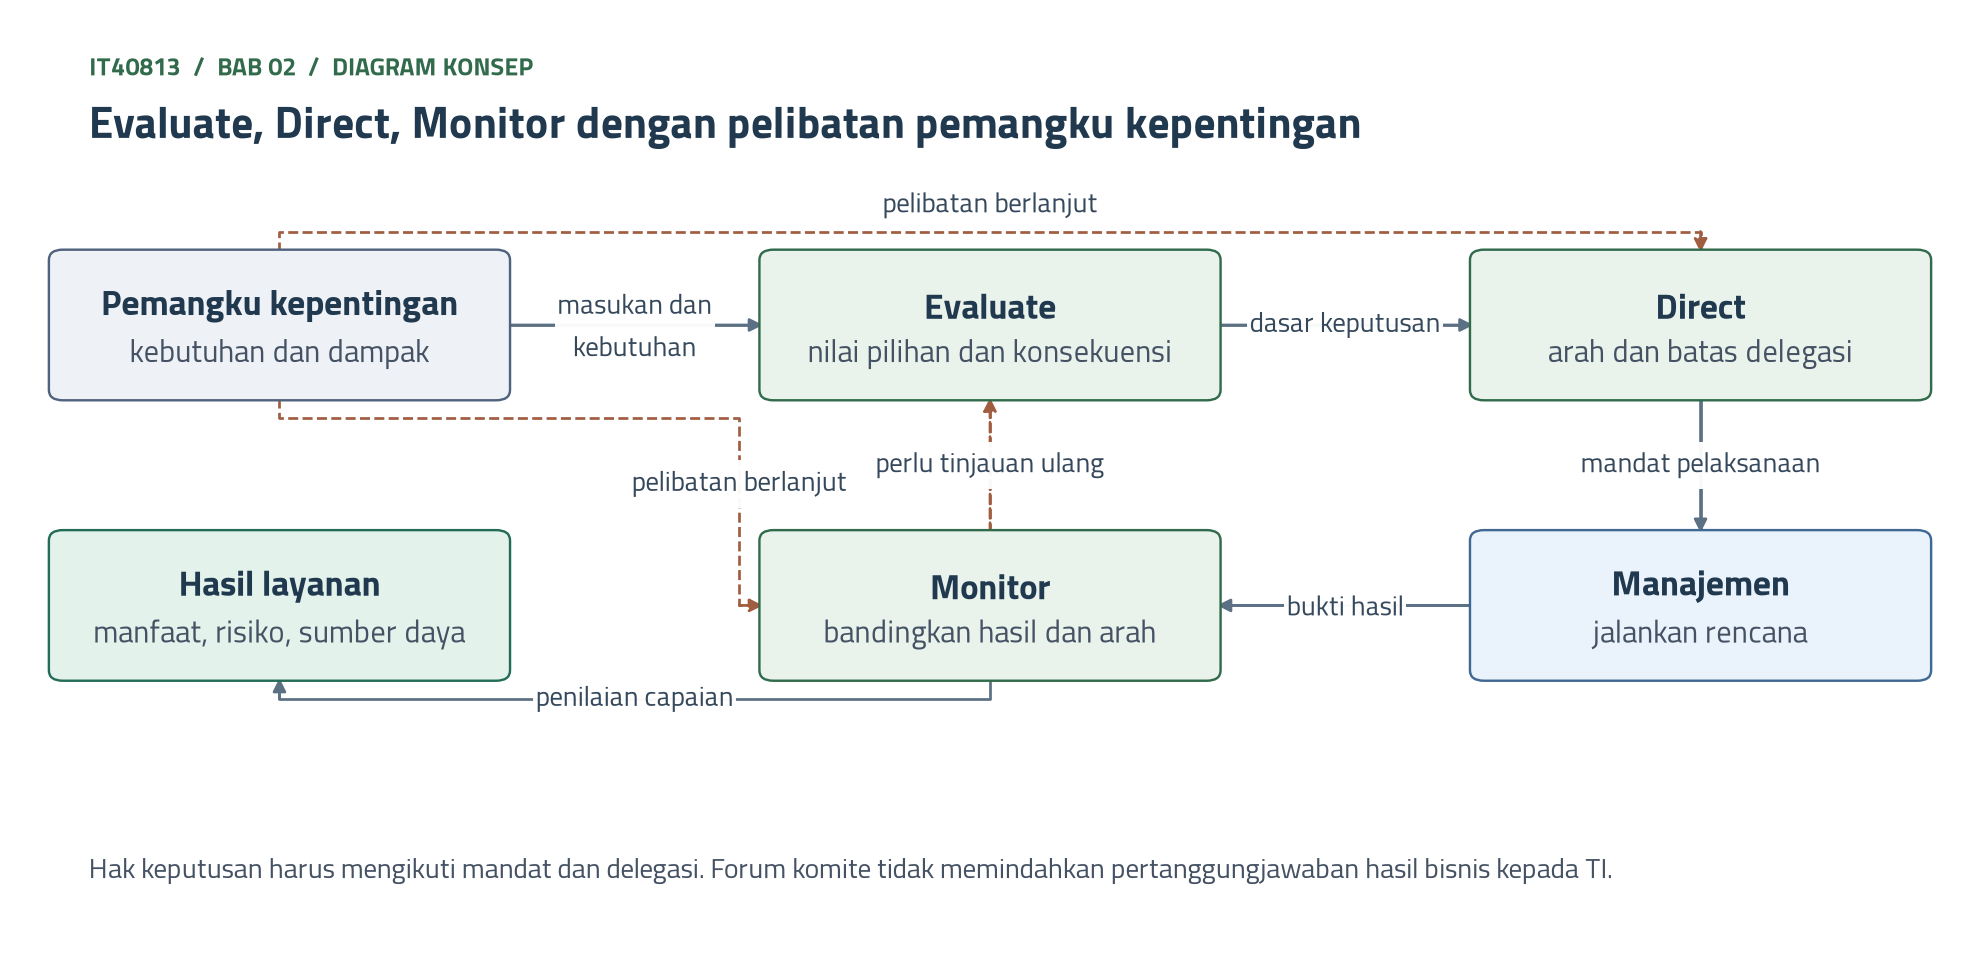
\includegraphics[width=\textwidth]{../figures/ch02-diagram-konsep.png}
  \caption{Evaluate, Direct, Monitor dengan pelibatan pemangku kepentingan}
  \label{fig:ch02-ilustrasi-bab}
\end{figure}
}{}

\section{Tata Kelola Korporat dan Posisi TI}

Pertanyaan pertama: di mana letak TI dalam tata kelola perusahaan? Tata kelola TI bukan
sistem yang berdiri sendiri. \textit{White paper} di situs komite ISO menyebutnya bagian yang
menyatu dengan tata kelola organisasi \cite{c02-iso-perubahan}. Karena itu, penelusuran
kewenangan dimulai dari organ perseroan, bukan dari struktur unit TI.

Pada perseroan terbatas Indonesia, direksi menjalankan pengurusan untuk kepentingan
perseroan, sesuai kebijakan yang dipandang tepat dalam batas undang-undang dan anggaran
dasar. Dewan komisaris mengawasi kebijakan dan jalannya pengurusan, lalu memberi nasihat
kepada direksi. Pembagian tugas antaranggota direksi ditetapkan rapat umum pemegang saham,
atau oleh direksi sendiri bila rapat umum tidak menetapkannya. Pembagian ini perlu dibaca
bersama anggaran dasar dan perubahan peraturan yang berlaku. Pasal 92 dan Pasal 108
Undang-Undang (UU) 40/2007 menjadi titik awal penelusuran, bukan alasan menyalin struktur
perusahaan lain \cite{c02-uu40}.

Organisasi tidak dapat memindahkan seluruh pertanggungjawaban pemanfaatan TI kepada kepala
TI atau vendor. Direktur pelayanan memiliki manfaat layanan. Direktur keuangan memiliki
pertimbangan pendanaan. Fungsi teknologi menjelaskan kelayakan. Komite memberi forum
koordinasi, sedangkan kewenangan hukum tetap mengikuti mandat.
Gambar~\ref{fig:ch02-organ-perseroan} memperlihatkan hubungan itu pada Medikara. Rincian di
bawah direksi adalah pengandaian, karena fakta dasar kasus tidak menyebut susunan
jabatannya.

\begin{figure}[!htb]
  \centering
  \begin{tikzpicture}[
  kotak/.style={draw, rounded corners, align=center, text width=2.85cm,
    minimum height=1.15cm, font=\scriptsize, fill=blue!8},
  panah/.style={-{Stealth[length=2mm]}, thick},
  keterangan/.style={font=\tiny, align=center, inner sep=1pt}
]
  \node[kotak, fill=praditagreen!15] (komisaris) at (0, 4.5)
    {\textbf{Dewan Komisaris}\\{\tiny\mdseries mengawasi dan\\memberi nasihat}};
  \node[kotak, fill=praditagreen!15] (direksi) at (4.45, 4.5)
    {\textbf{Direksi}\\{\tiny\mdseries mengurus perseroan\\dan menetapkan delegasi}};
  \node[kotak, fill=orange!12] (komite) at (8.9, 4.5)
    {\textbf{Komite pengarah TI}\\{\tiny\mdseries forum bermandat,\\bukan organ perseroan}};
  \node[kotak] (pemilik) at (2.225, 2.25)
    {\textbf{Pemilik layanan}\\{\tiny\mdseries direktur pelayanan:\\manfaat dan risiko}};
  \node[kotak] (manajemen) at (6.675, 2.25)
    {\textbf{Manajemen TI}\\{\tiny\mdseries kepala TI:\\kesiapan dan operasi}};
  \node[kotak, fill=green!10] (hasil) at (2.225, 0)
    {\textbf{Hasil layanan}\\{\tiny\mdseries waktu tunggu,\\mutu, dan biaya}};
  \node[kotak] (vendor) at (6.675, 0)
    {\textbf{Vendor}\\{\tiny\mdseries menjalankan pekerjaan\\sesuai kontrak}};
  \draw[panah] ([yshift=2mm]komisaris.east) -- node[keterangan, above]
    {pengawasan\\nasihat} ([yshift=2mm]direksi.west);
  \draw[panah] ([yshift=-2mm]direksi.west) -- node[keterangan, below]
    {laporan} ([yshift=-2mm]komisaris.east);
  \draw[panah] ([yshift=2mm]direksi.east) -- node[keterangan, above]
    {mandat} ([yshift=2mm]komite.west);
  \draw[panah] ([yshift=-2mm]komite.west) -- node[keterangan, below]
    {rekomendasi} ([yshift=-2mm]direksi.east);
  \draw[panah] (direksi.south) -- node[keterangan, fill=white] {delegasi}
    (pemilik.north);
  \draw[panah] (direksi.south) -- node[keterangan, fill=white] {delegasi}
    (manajemen.north);
  \draw[{Stealth[length=2mm]}-{Stealth[length=2mm]}, thick] (pemilik) --
    node[keterangan, above] {kebutuhan\\kesiapan} (manajemen);
  \draw[panah] (pemilik) -- node[keterangan, right] {memiliki\\manfaat} (hasil);
  \draw[panah] (manajemen) -- node[keterangan, right] {mengelola\\kontrak} (vendor);
  \draw[panah] (vendor) -- node[keterangan, above] {pekerjaan} (hasil);
\end{tikzpicture}

  \caption{Organ perseroan, forum komite, dan pemilik hasil pada pengandaian Medikara}
  \label{fig:ch02-organ-perseroan}
\end{figure}

Pengelola rumah sakit dapat meminta penasihat menilai mutu bangunan. Penasihat membantu
menimbang pilihan, tetapi tanda tangan kontrak dan tanggung jawab pengelolaan tetap
mengikuti kewenangan organisasi. Membentuk forum tambahan tidak otomatis memindahkan
tanggung jawab.

Dua contoh penerapannya:
\begin{enumerate}
  \item Misalkan anggaran dasar Medikara mewajibkan persetujuan dewan komisaris untuk
  pengadaan di atas Rp5 miliar. Pasal 117 memberi ruang bagi pengaturan seperti itu.
  Investasi Rp8 miliar melewati batas tersebut. Dewan komisaris kemudian meminta laporan
  risiko modernisasi lima rumah sakit setiap triwulan, atau 4 kali setahun. Direksi tetap
  mengurus program dan menindaklanjuti temuan yang masuk kewenangannya.
  \item Misalkan direktur pelayanan menjadi pemilik manfaat investasi Rp8 miliar. Waktu
  tunggu dipengaruhi jadwal sekitar 640 dokter dan alur kerja di 5 rumah sakit. Kepala TI
  memimpin 52 staf TI dan mengelola kesiapan teknis, tetapi tidak berwenang mengubah jadwal
  dokter. Kepala TI juga tidak sendirian menerima risiko perubahan alur klinis.
\end{enumerate}

Tabel~\ref{tab:ch02-korporat} merangkum peran korporat dan pemanfaatan TI.
\begin{table}[!htb]
  \centering\small
  \caption{Peran korporat dan pemanfaatan TI}\label{tab:ch02-korporat}
  \begin{tabularx}{\textwidth}{|>{\raggedright\arraybackslash}p{0.22\textwidth}|>{\raggedright\arraybackslash}X|>{\raggedright\arraybackslash}X|}
    \hline
    \textbf{Peran} & \textbf{Tanggung jawab contoh} & \textbf{Bukti yang dicari} \\ \hline
    Dewan komisaris & Pengawasan dan nasihat & Notulen pengawasan \\ \hline
    Direksi & Arah, investasi, dan pengurusan & Keputusan serta delegasi \\ \hline
    Pemilik layanan & Hasil dan risiko layanan & Ukuran manfaat \\ \hline
    Manajemen TI & Pelaksanaan serta operasi & Rencana dan laporan kontrol \\ \hline
    Vendor & Pekerjaan sesuai kontrak & Berita acara dan laporan layanan \\ \hline
  \end{tabularx}
\end{table}

\subsection*{Pengurusan dan pengawasan}

Dua hal sering tertukar: pengurusan dan pengawasan. Pembagiannya begini. Pengurusan memilih
tindakan dan menjalankannya. Pengawasan memeriksa kebijakan dan jalannya pengurusan, lalu
memberi nasihat. Komisaris yang memilih vendor Medikara+ sedang masuk ke wilayah pengurusan.
Pasal 118 hanya membuka jalan itu berdasarkan anggaran dasar atau keputusan rapat umum
pemegang saham, untuk keadaan dan jangka waktu tertentu \cite{c02-uu40}.

Pembagian ini menimbulkan kesulitan istilah. Standar internasional memakai kata badan
pengarah (\textit{governing body}) atau \textit{board}. The Institute of Internal Auditors
(IIA) memakai \textit{board} untuk berbagai bentuk badan pengarah beserta komitenya
\cite{iia-tlm2026}. Perseroan Indonesia memisahkan dua organ, sehingga istilah itu tidak
dapat diterjemahkan satu lawan satu. Tabel~\ref{tab:ch02-pemetaan} memberi pemetaan kerja
untuk bab ini. Pemetaan itu penafsiran bab ini, bukan isi standar. Tim tetap perlu
mencocokkannya dengan anggaran dasar organisasi.

\begin{table}[!htb]
  \centering\small
  \caption{Pemetaan kerja tugas tata kelola pada dua organ perseroan}
  \label{tab:ch02-pemetaan}
  \begin{tabularx}{\textwidth}{|>{\raggedright\arraybackslash}p{0.2\textwidth}|>{\raggedright\arraybackslash}X|>{\raggedright\arraybackslash}X|}
    \hline
    \textbf{Tugas} & \textbf{Direksi} & \textbf{Dewan komisaris} \\ \hline
    \textit{Evaluate} & Menilai opsi investasi dan dampaknya & Memberi nasihat; menyetujui
    bila anggaran dasar menetapkan \\ \hline
    \textit{Direct} & Menetapkan arah, pemilik manfaat, dan batas delegasi & Tidak memberi
    perintah operasional \\ \hline
    \textit{Monitor} & Memantau hasil dan memerintahkan koreksi & Mengawasi kebijakan dan
    jalannya pengurusan \\ \hline
    Pelibatan & Mengatur saluran masukan pasien, klinisi, dan unit lokal & Menanyakan
    apakah pihak terdampak sudah didengar \\ \hline
  \end{tabularx}
\end{table}

\subsection*{Akuntabilitas tidak ikut berpindah}

Bila pekerjaan didelegasikan atau dialihkan ke vendor, apakah tanggung jawabnya ikut
berpindah? Tidak seluruhnya. Direksi bertanggung jawab atas pengurusan, dan dewan komisaris
bertanggung jawab atas pengawasan. Anggota kedua organ dapat bertanggung jawab secara
pribadi atas kerugian perseroan bila bersalah atau lalai. Pasal 97 ayat (5) menyebut syarat
pembebasan bagi anggota direksi, antara lain itikad baik, kehati-hatian, dan tidak adanya
benturan kepentingan \cite{c02-uu40}. IIA menyatakan alih daya tidak mengubah akuntabilitas
\textit{board} untuk memastikan kegiatan yang dialihkan berjalan efektif
\cite{iia-tlm2026}. Pernyataan IIA itu membahas kegiatan asurans dan nasihat. Bab ini
memakai logika yang serupa untuk pekerjaan vendor.

Keadaan ini punya dua konsekuensi. Pertama, catatan keputusan bernilai sebagai
pertanggungjawaban. Notulen yang memuat opsi, alasan, dan deklarasi kepentingan membantu
menunjukkan kehati-hatian, meskipun tidak menjamin pembebasan tanggung jawab. Bagian ini
bukan nasihat hukum. Kedua, kontrak menetapkan tugas vendor, tetapi tidak menghapus
kewajiban organisasi menetapkan siapa memantau hasil. Data latihan Bab 1 memperlihatkan
akibatnya: kontrak selesai, akun dukungan tetap aktif, dan 1.240 rekam kunjungan terbaca
selama 8 malam.

\begin{kasus}[title={Kasus Medikara Health: Pertanyaan Komisaris pada Laporan Triwulan}]
Misalkan laporan triwulan menyebut pemasangan Medikara+ sudah mencapai 90 persen. Dewan
komisaris mengajukan tiga pertanyaan. Siapa pemilik manfaat? Berapa selisih hasil terhadap
target? Apa keputusan yang menunggu direksi? Jawaban pertama ternyata berbeda antara
direktur pelayanan dan kepala TI. Jawaban kedua baru tersedia setelah data 5 rumah sakit
dikumpulkan: 38 menit, dari target 25 menit. Jawaban ketiga belum ada.

Dewan komisaris tidak memilih perbaikan, karena memilih perbaikan termasuk pengurusan.
Dewan komisaris menasihati direksi agar menetapkan satu pemilik manfaat dan membawa pilihan
koreksi pada triwulan berikutnya. Direksi lalu menunjuk direktur pelayanan sebagai pemilik
manfaat, sesuai pembagian tugas yang berlaku.
\end{kasus}

\section{ISO/IEC 38500:2024 dan Model Evaluate, Direct, Monitor}

Setelah organnya jelas, apa yang seharusnya dikerjakan? ISO/IEC 38500:2024 memberi panduan
bagi badan pengarah tentang penggunaan TI dalam organisasi \cite{iso38500-2024}. Teks
standar ini berbayar, sehingga rincian berikut mengikuti \textit{white paper} perbedaan
edisi yang terbit di situs komite penyusunnya. Halaman itu memuat penafian bahwa isinya
dikelola pihak ketiga, sehingga tim yang memakainya untuk penilaian formal tetap perlu
memeriksa teks standar \cite{c02-iso-perubahan}.

Edisi 2024 selaras dengan ISO 37000 tentang tata kelola organisasi. Prinsipnya berubah dari
enam menjadi sebelas. Modelnya menambahkan pelibatan pemangku kepentingan
(\textit{engage stakeholders}) di samping tiga tugas EDM. Fokusnya juga bergeser. Tata
kelola tidak lagi dibahas terutama sebagai kerja badan pengarah, tetapi sebagai sesuatu yang
dijalankan di seluruh organisasi, dengan manajemen bekerja dalam kerangka yang ditetapkan
badan pengarah \cite{c02-iso-perubahan}. Tabel~\ref{tab:ch02-edisi} merangkum perbedaannya.

\begin{table}[!htb]
  \centering\small
  \caption{Perbedaan ISO/IEC 38500 edisi 2015 dan edisi 2024}\label{tab:ch02-edisi}
  \begin{tabularx}{\textwidth}{|>{\raggedright\arraybackslash}p{0.18\textwidth}|>{\raggedright\arraybackslash}X|>{\raggedright\arraybackslash}X|}
    \hline
    \textbf{Aspek} & \textbf{Edisi 2015} & \textbf{Edisi 2024} \\ \hline
    Prinsip & Enam: tanggung jawab, strategi, akuisisi, kinerja, kesesuaian, perilaku
    manusia & Sebelas, mengikuti prinsip ISO 37000 \\ \hline
    Model & \textit{Evaluate}, \textit{Direct}, dan \textit{Monitor} oleh badan pengarah &
    Ditambah pelibatan pemangku kepentingan, di atas manajemen TI \\ \hline
    Letak tata kelola & Terutama pada badan pengarah & Di seluruh organisasi, dalam kerangka
    dari badan pengarah \\ \hline
    Kerangka & Konsepnya pertama muncul pada ISO/IEC 38502 & Enam unsur: arah, kapabilitas,
    kebijakan, delegasi, kinerja, akuntabilitas \\ \hline
  \end{tabularx}
\end{table}

Banyak materi daring masih memakai enam prinsip edisi 2015. Daftar itu tidak boleh diberi
label edisi 2024. Tabel~\ref{tab:ch02-prinsip} memuat sebelas prinsip edisi 2024, dengan
kelompok \textit{primary} (utama), \textit{foundational} (dasar), dan \textit{enabling}
(pemungkin). Kolom pertanyaan adalah penerapan bab ini berupa pertanyaan keputusan, bukan
kutipan persyaratan standar.

\begin{table}[!htb]
  \centering\small
  \caption{Sebelas prinsip ISO/IEC 38500:2024 dan pertanyaan penerapannya}
  \label{tab:ch02-prinsip}
  \begin{tabularx}{\textwidth}{|>{\raggedright\arraybackslash}p{0.16\textwidth}|>{\raggedright\arraybackslash}p{0.27\textwidth}|>{\raggedright\arraybackslash}X|}
    \hline
    \textbf{Kelompok} & \textbf{Prinsip} & \textbf{Pertanyaan bagi TI Medikara} \\ \hline
    Utama & Tujuan & Layanan pasien mana yang dilayani TI? \\ \hline
    Dasar & Pembentukan nilai & Nilai apa yang dihasilkan Medikara+? \\ \hline
    Dasar & Strategi & Apakah investasi mendukung ``Satu Pasien, Satu Rekam Medis''? \\
    \hline
    Dasar & Pengawasan & Siapa memeriksa jalannya program? \\ \hline
    Dasar & Akuntabilitas & Siapa menjawab bila target tidak tercapai? \\ \hline
    Pemungkin & Pelibatan pemangku kepentingan & Apakah pasien dan klinisi sudah didengar?
    \\ \hline
    Pemungkin & Kepemimpinan & Siapa memberi contoh dalam memakai data dan aturan? \\
    \hline
    Pemungkin & Data dan keputusan & Apakah keputusan memakai data yang dapat diperiksa? \\
    \hline
    Pemungkin & Tata kelola risiko & Risiko mana yang diterima, dan oleh siapa? \\ \hline
    Pemungkin & Tanggung jawab sosial & Siapa terdampak di luar organisasi? \\ \hline
    Pemungkin & Kelangsungan dan kinerja dari waktu ke waktu & Apakah layanan tetap bertahan
    setelah proyek selesai? \\ \hline
  \end{tabularx}
\end{table}

Prinsip tidak berjalan tanpa kerangka. \textit{White paper} yang sama menyebut enam unsur
kerangka tata kelola menurut edisi 2024 \cite{c02-iso-perubahan}. Keenam unsur itu menjadi
daftar periksa yang berguna saat menilai sebuah organisasi.
Tabel~\ref{tab:ch02-kerangka} menerapkannya pada pengandaian Medikara.

\begin{table}[!htb]
  \centering\small
  \caption{Enam unsur kerangka tata kelola pada pengandaian Medikara}
  \label{tab:ch02-kerangka}
  \begin{tabularx}{\textwidth}{|>{\raggedright\arraybackslash}p{0.2\textwidth}|>{\raggedright\arraybackslash}X|}
    \hline
    \textbf{Unsur} & \textbf{Bentuk pada Medikara} \\ \hline
    Arah & Strategi ``Satu Pasien, Satu Rekam Medis'' 2026 sampai 2030 \\ \hline
    Kapabilitas & 52 staf TI dengan tim platform 6 orang, ditambah vendor Medikara+ \\
    \hline
    Kebijakan & Aturan akses vendor dan standar integrasi \\ \hline
    Delegasi & Batas biaya dan toleransi 10 persen, dijelaskan pada seksi berikutnya \\
    \hline
    Kinerja & Waktu tunggu pendaftaran dari 40 menjadi 25 menit \\ \hline
    Akuntabilitas & Direktur pelayanan sebagai pemilik manfaat, dengan catatan keputusan \\
    \hline
  \end{tabularx}
\end{table}

Evaluasi memerlukan alternatif nyata, termasuk menunda atau menghentikan. Arahan menyebut
batas biaya, pemilik manfaat, risiko yang diterima, dan kondisi penghentian. Pemantauan
membandingkan hasil terhadap arahan dan dapat memicu evaluasi ulang. Pertanyaan kemudian
muncul: siapa perlu dilibatkan? Pihak yang memakai layanan dan menanggung akibat harus
memiliki saluran masukan. Gambar~\ref{fig:ch02-alur} memperlihatkan siklus itu dengan angka
pengandaian Medikara.

\begin{figure}[!htb]
  \centering
  \begin{tikzpicture}[
  kotak/.style={draw, rounded corners, align=center, text width=2.85cm,
    minimum height=1.25cm, font=\scriptsize, fill=blue!8},
  panah/.style={-{Stealth[length=2mm]}, thick},
  keterangan/.style={font=\tiny, align=center, inner sep=1pt}
]
  \node[kotak, fill=praditagreen!15] (pemangku) at (0, 2.6)
    {\textbf{Pemangku}\\\textbf{kepentingan}\\{\tiny\mdseries kebutuhan dan
    dampak:\\pasien, klinisi, unit lokal}};
  \node[kotak] (evaluate) at (4.4, 2.6)
    {\textbf{\textit{Evaluate}}\\{\tiny\mdseries nilai pilihan dan konsekuensi:\\Rp8
    miliar atau Rp6 miliar}};
  \node[kotak] (direct) at (8.8, 2.6)
    {\textbf{\textit{Direct}}\\{\tiny\mdseries arah dan batas delegasi:\\batas Rp8,8
    miliar,\\target 25 menit}};
  \node[kotak] (manajemen) at (8.8, 0)
    {\textbf{Manajemen}\\{\tiny\mdseries jalankan rencana:\\pemasangan di 5 rumah
    sakit}};
  \node[kotak, fill=orange!12] (monitor) at (4.4, 0)
    {\textbf{\textit{Monitor}}\\{\tiny\mdseries bandingkan hasil dan arah:\\38 menit,
    target 25 menit}};
  \node[kotak, fill=green!10] (hasil) at (0, 0)
    {\textbf{Hasil layanan}\\{\tiny\mdseries manfaat, risiko, sumber daya:\\baru 13,3
    persen target}};
  \draw[panah] (pemangku) -- node[keterangan, above]
    {masukan\\dan\\kebutuhan} (evaluate);
  \draw[panah] (evaluate) -- node[keterangan, above]
    {dasar\\keputusan} (direct);
  \draw[panah] (direct) -- node[keterangan, right]
    {mandat\\pelaksanaan} (manajemen);
  \draw[panah] (manajemen) -- node[keterangan, above]
    {bukti\\hasil} (monitor);
  \draw[panah] (monitor) -- node[keterangan, above]
    {penilaian\\capaian} (hasil);
  \draw[panah, dashed] (monitor) -- node[keterangan, right]
    {perlu\\tinjauan\\ulang} (evaluate);
  \draw[panah, densely dotted] (pemangku.south east) -- (monitor.north west);
  \draw[panah, densely dotted] (pemangku.north) -- ++(0, 0.42) -|
    node[keterangan, above, pos=0.25] {pelibatan berlanjut pada ketiga tugas}
    (direct.north);
\end{tikzpicture}

  \caption{Siklus EDM dengan pelibatan pemangku kepentingan pada keputusan Medikara+}
  \label{fig:ch02-alur}
\end{figure}

Panitia renovasi sekolah membandingkan pilihan sebelum memilih kontraktor, menetapkan batas
anggaran dan keselamatan, lalu memeriksa penggunaan ruangan setelah selesai. Guru serta
murid memberi masukan karena mereka mengalami akibat keputusan setiap hari.

Dua contoh penerapannya:
\begin{enumerate}
  \item Misalkan dua opsi aplikasi pasien berbiaya Rp8 miliar dan Rp6 miliar, dengan masa
  pakai 5 tahun. Biaya per tahunnya Rp1,6 miliar dan Rp1,2 miliar. Dengan 336.000 janji
  temu per tahun, biaya per janji temu sekitar Rp4.760 dan Rp3.570. Misalkan opsi pertama
  menargetkan penurunan 15 menit, dan opsi kedua 10 menit. Penghematannya 84.000 jam dan
  56.000 jam per tahun, atau sekitar Rp19.000 dan Rp21.400 per jam. Evaluasi juga menilai
  keselamatan serta kemampuan adopsi, bukan memilih angka terendah secara otomatis.
  \item Misalkan target waktu tunggu turun dari 40 menjadi 25 menit, dengan batas biaya
  Rp8,8 miliar berdasarkan toleransi 10 persen seperti pada Bab 1. Hasil tiga bulan masih
  38 menit, atau baru 2 dari 15 menit yang ditargetkan (13,3 persen). Pemantauan memicu
  peninjauan proses, alokasi petugas, dan rancangan aplikasi. Bila biaya naik 27 persen,
  sesuai rata-rata pada Bab 1, nilainya Rp10,16 miliar dan keputusan kembali ke direksi.
\end{enumerate}

\subsection*{Dua pemantauan yang sering tertukar}

Dua hal pada EDM sering tertukar: \textit{Monitor} sebagai tugas tata kelola dan pemantauan
harian oleh manajemen. Pembagiannya begini. Manajemen memantau jalannya pekerjaan agar
rencana terlaksana. Badan pengarah memantau apakah arah masih benar dan hasilnya sesuai.
Control Objectives for Information and Related Technologies (COBIT) juga memisahkan
keduanya \cite{cobit2019-intro}, dan Bab 4 membahas rinciannya.

Misalkan tiap rumah sakit mengirim laporan pekanan. Lima rumah sakit menghasilkan 260
laporan setahun. Manajemen membaca semuanya untuk memperbaiki operasi. Direksi cukup
menerima 4 laporan triwulan yang memuat hasil, risiko, dan keputusan yang diperlukan. Bila
direksi membaca 260 laporan, direksi masuk ke pekerjaan manajemen dan justru kehilangan
pandangan atas arah. Tabel~\ref{tab:ch02-edm} merangkum pertanyaan pada tingkat tata kelola.

\begin{table}[!htb]
  \centering\small
  \caption{Pertanyaan EDM untuk keputusan investasi}\label{tab:ch02-edm}
  \begin{tabularx}{\textwidth}{|>{\raggedright\arraybackslash}p{0.22\textwidth}|>{\raggedright\arraybackslash}X|>{\raggedright\arraybackslash}X|}
    \hline
    \textbf{Tugas} & \textbf{Pertanyaan} & \textbf{Contoh hasil} \\ \hline
    \textit{Evaluate} & Apa masalah, opsi, dan dampaknya? & Perbandingan dua opsi \\ \hline
    \textit{Direct} & Siapa berwenang dan apa batasnya? & Mandat dan pemilik manfaat \\
    \hline
    \textit{Monitor} & Apakah hasil memenuhi arahan? & Laporan manfaat dan tindakan \\
    \hline
    Pelibatan pihak & Siapa belum didengar? & Masukan pasien dan klinisi \\ \hline
  \end{tabularx}
\end{table}

\section{Hak Keputusan TI}

Pertanyaan berikutnya: siapa tepatnya yang memutuskan? Hak keputusan menyatakan siapa
memberi masukan dan siapa menetapkan keputusan akhir pada domain tertentu. Weill
memandang tata kelola TI sebagai penetapan hak keputusan dan akuntabilitas untuk mendorong
perilaku yang diinginkan dalam penggunaan TI. Kajiannya mencakup lebih dari 250 perusahaan
di 23 negara \cite{c02-weill-misqe}. Weill dan Ross membedakan lima keputusan: prinsip TI,
arsitektur, infrastruktur, kebutuhan aplikasi bisnis, serta investasi dan prioritas. Arketipe
menggambarkan lokasi kewenangan: monarki bisnis, monarki TI, feodal, federal, duopoli, dan
anarki \cite{weill2004,c02-weill-misqe}.

Monarki bisnis menempatkan keputusan pada pimpinan bisnis, monarki TI pada pimpinan
teknologi, dan feodal pada unit bisnis masing-masing. Federal menggabungkan pusat dan unit.
Duopoli menggabungkan teknologi dengan satu kelompok bisnis. Anarki berarti keputusan
individual. Arketipe adalah lensa analisis. Matriks organisasi tetap harus menyebut jabatan
dan batas delegasi yang konkret. Tabel~\ref{tab:ch02-arketipe} memberi contoh dan akibat
tiap arketipe.

\begin{table}[!htb]
  \centering\small
  \caption{Enam arketipe hak keputusan dengan contoh pengandaian Medikara}
  \label{tab:ch02-arketipe}
  \begin{tabularx}{\textwidth}{|>{\raggedright\arraybackslash}p{0.15\textwidth}|>{\raggedright\arraybackslash}p{0.21\textwidth}|>{\raggedright\arraybackslash}X|>{\raggedright\arraybackslash}X|}
    \hline
    \textbf{Arketipe} & \textbf{Letak keputusan} & \textbf{Misalkan di Medikara} &
    \textbf{Akibat} \\ \hline
    Monarki bisnis & Pimpinan bisnis senior & Direksi memutuskan prinsip identitas pasien &
    Arah kuat; perlu masukan kelayakan \\ \hline
    Monarki TI & Pimpinan TI & Kepala TI memutuskan standar integrasi & Standar konsisten;
    manfaat layanan kurang terwakili \\ \hline
    Feodal & Tiap unit bisnis & Tiap rumah sakit memilih sistem sendiri & Cepat di tingkat
    lokal; 5 versi Sistem Informasi Manajemen Rumah Sakit (SIMRS) sulit disatukan \\ \hline
    Federal & Pusat bersama unit & Direktur pelayanan bersama 5 direktur rumah sakit & Pusat
    dan unit terwakili; kesepakatan lebih lama \\ \hline
    Duopoli TI & TI bersama satu kelompok bisnis & Kepala TI bersama direktur pelayanan &
    Nilai dan kelayakan dinilai bersama; perlu aturan bila tidak sepakat \\ \hline
    Anarki & Individu atau kelompok kecil & Unit menyusun laporan dengan \textit{spreadsheet}
    sendiri & Murah di awal; data tersebar \\ \hline
  \end{tabularx}
\end{table}

Lima keputusan dan enam arketipe membentuk sebuah matriks.
Gambar~\ref{fig:ch02-matriks-arketipe} mengisinya dengan pengandaian Medikara. Misalkan kotak
merah menunjukkan pemutus saat ini, sedangkan lingkaran menunjukkan susunan yang diusulkan.
Tiga dari lima kotak merah berada pada kolom feodal, sejalan dengan versi SIMRS yang berbeda
di tiap rumah sakit. Makin banyak kotak pada kolom itu, makin besar hambatan bagi strategi
satu rekam medis.

\begin{figure}[!htb]
  \centering
  \begin{tikzpicture}[
  kolom/.style={font=\scriptsize\bfseries, align=center, text width=1.28cm},
  baris/.style={font=\scriptsize, align=left, text width=3.1cm, anchor=west},
  pemutus/.style={circle, fill=praditagreen, draw=black, minimum size=3mm,
    inner sep=0pt},
  masukan/.style={circle, fill=white, draw=black, thick, minimum size=3mm,
    inner sep=0pt},
  kini/.style={rectangle, fill=red!22, draw=black, minimum size=2.8mm,
    inner sep=0pt}
]
  % Kisi 6 kolom arketipe dan 5 baris keputusan; lebar total 11,7 cm.
  \fill[praditagreen!15] (0, 0) rectangle (11.7, 0.85);
  \draw[gray] (0, -3.5) grid[xstep=11.7, ystep=0.7] (11.7, 0);
  \foreach \posisi in {3.3, 4.7, 6.1, 7.5, 8.9, 10.3, 11.7} {
    \draw[gray] (\posisi, -3.5) -- (\posisi, 0.85);
  }
  \draw[gray] (0, -3.5) rectangle (11.7, 0.85);
  \node[baris, font=\scriptsize\bfseries] at (0, 0.425) {Keputusan};
  \node[kolom] at (4.0, 0.425) {Monarki bisnis};
  \node[kolom] at (5.4, 0.425) {Monarki TI};
  \node[kolom] at (6.8, 0.425) {Feodal};
  \node[kolom] at (8.2, 0.425) {Federal};
  \node[kolom] at (9.6, 0.425) {Duopoli TI};
  \node[kolom] at (11.0, 0.425) {Anarki};
  \node[baris] at (0, -0.35) {Prinsip TI};
  \node[baris] at (0, -1.05) {Arsitektur TI};
  \node[baris] at (0, -1.75) {Infrastruktur TI};
  \node[baris] at (0, -2.45) {Kebutuhan aplikasi bisnis};
  \node[baris] at (0, -3.15) {Investasi dan prioritas TI};
  % Prinsip TI
  \node[pemutus] at (4.0, -0.35) {};
  \node[masukan] at (8.2, -0.35) {};
  \node[kini] at (5.4, -0.35) {};
  % Arsitektur TI
  \node[pemutus] at (5.4, -1.05) {};
  \node[masukan] at (8.2, -1.05) {};
  \node[kini] at (6.8, -1.05) {};
  % Infrastruktur TI
  \node[pemutus] at (5.4, -1.75) {};
  \node[masukan] at (9.6, -1.75) {};
  \node[kini] at (6.8, -1.75) {};
  % Kebutuhan aplikasi bisnis
  \node[pemutus] at (8.2, -2.45) {};
  \node[masukan] at (6.55, -2.45) {};
  \node[kini] at (7.05, -2.45) {};
  % Investasi dan prioritas TI
  \node[pemutus] at (4.0, -3.15) {};
  \node[masukan] at (9.6, -3.15) {};
  \node[kini] at (5.4, -3.15) {};
  % Keterangan penanda
  \node[pemutus] at (0.2, -3.95) {};
  \node[font=\scriptsize, anchor=west] at (0.4, -3.95) {pemutus usulan};
  \node[masukan] at (3.6, -3.95) {};
  \node[font=\scriptsize, anchor=west] at (3.8, -3.95) {pemberi masukan usulan};
  \node[kini] at (7.9, -3.95) {};
  \node[font=\scriptsize, anchor=west] at (8.1, -3.95) {pemutus saat ini};
\end{tikzpicture}

  \caption{Matriks hak keputusan pengandaian Medikara: lima keputusan dan enam arketipe
  menurut Weill dan Ross}
  \label{fig:ch02-matriks-arketipe}
\end{figure}

Memilih menu makan bersama memberi semua peserta kesempatan menyampaikan alergi dan
preferensi. Satu koordinator tetap perlu mengonfirmasi pesanan dalam anggaran yang
disepakati. Banyak masukan tidak mengharuskan banyak pemesan akhir.

Dua contoh penerapannya:
\begin{enumerate}
  \item Misalkan investasi Medikara+ diputuskan direksi berdasarkan rekomendasi bersama
  direktur pelayanan dan kepala TI. Polanya menyerupai duopoli pada tahap rekomendasi,
  dengan persetujuan akhir mengikuti delegasi investasi. Karena Rp8 miliar melewati batas
  Rp5 miliar pada pengandaian sebelumnya, dewan komisaris ikut memberi persetujuan.
  \item Misalkan lima rumah sakit membeli pengelolaan identitas sendiri seharga Rp700 juta
  per rumah sakit, atau Rp3,5 miliar seluruhnya. Pola feodal memberi kecepatan lokal, tetapi
  menyulitkan sasaran identitas pasien tunggal. Platform bersama Rp2 miliar menghemat Rp1,5
  miliar, dengan konsekuensi rumah sakit terakhir menunggu lebih lama.
\end{enumerate}

\subsection*{Tidak ada satu susunan terbaik}

Weill melaporkan bahwa perusahaan unggul berbeda satu sama lain dan berbeda dari perusahaan
rata-rata. Perusahaan yang unggul pada pertumbuhan cenderung memberi lebih banyak hak
keputusan kepada unit bisnis. Perusahaan yang unggul pada laba lebih terpusat, dengan
pimpinan bisnis senior memutuskan keputusan TI utama \cite{c02-weill-misqe}. Halaman MIT
Center for Information Systems Research menyebut perusahaan dengan tata kelola TI yang unggul
memiliki laba lebih dari 25 persen di atas perusahaan dengan tata kelola buruk, pada tujuan
strategis yang sama \cite{weill2004}.

Angka 25 persen itu menggambarkan perbedaan antarkelompok perusahaan. Angka itu bukan janji
bahwa Medikara akan menaikkan laba 25 persen setelah membuat matriks. Pesan yang dapat
dipakai adalah kesesuaian: letak keputusan mengikuti tujuan kinerja. Medikara mengejar satu
rekam medis lintas fasilitas, sehingga keputusan identitas pasien lebih wajar terpusat. Alur
pendaftaran bergantung pada kondisi tiap rumah sakit, sehingga pola federal lebih masuk akal.

\subsection*{Masukan, veto, dan keputusan akhir}

Dua hal sering tertukar. Hak memberi masukan tidak sama dengan hak memveto. Masukan wajib
didengar, tetapi boleh tidak diikuti dengan alasan tertulis. Veto menghentikan keputusan,
sehingga harus ditulis eksplisit dan dibatasi. Bila semua pihak disebut pemutus, tanggung
jawab justru kabur. Setiap keputusan perlu satu kewenangan akhir yang jelas, sekalipun
keputusan dicapai melalui musyawarah atau badan kolektif.

Hitungan sederhana memperlihatkan alasannya. Misalkan empat pihak masing-masing memegang
veto, dan tiap pihak menyetujui 90 persen usulan secara terpisah. Peluang satu usulan lolos
adalah 0,9 pangkat 4, atau sekitar 65,6 persen. Sekitar sepertiga usulan berhenti, meskipun tiap
pihak terlihat mudah setuju. Veto sebaiknya diberikan untuk alasan yang sempit, misalnya
kepala rekam medis menghentikan pembukaan data pasien ke mitra bila dasar pemrosesannya belum
ada. Tabel~\ref{tab:ch02-hak} memperlihatkan pemisahan masukan dan keputusan pada empat
keputusan.

\begin{table}[!htb]
  \centering\small
  \caption{Contoh matriks hak keputusan}\label{tab:ch02-hak}
  \begin{tabularx}{\textwidth}{|>{\raggedright\arraybackslash}p{0.24\textwidth}|>{\raggedright\arraybackslash}X|>{\raggedright\arraybackslash}X|>{\raggedright\arraybackslash}p{0.2\textwidth}|}
    \hline
    \textbf{Keputusan} & \textbf{Pemberi masukan} & \textbf{Pemutus akhir} &
    \textbf{Pengawas} \\ \hline
    Prinsip identitas pasien & Layanan, data, dan TI & Direksi & Dewan komisaris \\ \hline
    Standar arsitektur & Pemilik aplikasi dan keamanan & Kepala TI lewat forum berdelegasi
    jelas & Komite pengarah TI \\ \hline
    Investasi Medikara+ & Layanan, TI, dan keuangan & Direksi sesuai batas & Dewan komisaris
    \\ \hline
    Akses vendor harian & Keamanan, kepala TI, dan pemilik data & Pemilik Medikara+ &
    Audit internal \\ \hline
  \end{tabularx}
\end{table}

Matriks perlu ditemani batas delegasi, karena tidak semua keputusan investasi layak naik ke
direksi. Tabel~\ref{tab:ch02-delegasi} memberi contoh yang sejalan dengan Bab 1, ketika direksi
menyetujui integrasi Rp450 juta per tahun dengan toleransi 10 persen. Semua angka adalah
pengandaian, bukan batas hukum.

\begin{table}[!htb]
  \centering\small
  \caption{Contoh batas delegasi keputusan TI pada pengandaian Medikara}
  \label{tab:ch02-delegasi}
  \begin{tabularx}{\textwidth}{|>{\raggedright\arraybackslash}p{0.28\textwidth}|>{\raggedright\arraybackslash}X|>{\raggedright\arraybackslash}p{0.27\textwidth}|}
    \hline
    \textbf{Nilai keputusan} & \textbf{Pemutus akhir} & \textbf{Laporan} \\ \hline
    Sampai Rp100 juta & Kepala TI, dengan masukan pemilik layanan & Ringkasan triwulan ke komite \\
    \hline
    Di atas Rp100 juta sampai Rp400 juta & Komite pengarah TI, sesuai mandat direksi &
    Notulen ke direksi \\ \hline
    Di atas Rp400 juta sampai Rp5 miliar & Direksi & Laporan triwulan ke dewan komisaris \\
    \hline
    Di atas Rp5 miliar & Direksi dengan persetujuan dewan komisaris, bila anggaran dasar
    menetapkan & Laporan triwulan ke dewan komisaris \\ \hline
    Kenaikan di atas 10 persen & Kembali ke pemutus awal & Alasan dan pilihan koreksi \\
    \hline
  \end{tabularx}
\end{table}

\begin{kasus}[title={Kasus Medikara Health: Siapa Mencabut Akun Vendor?}]
Risiko R-01 pada Bab 1 adalah akses vendor yang berlebihan. Audit memeriksa 30 dari 120 akun
vendor dan menemukan 6 akun aktif setelah penugasan berakhir. Peninjauan bulan berikutnya
mencabut 24 akun. Angka itu menjawab apa yang terjadi, tetapi belum menjawab siapa yang
berwenang.

Misalkan tim menyusun hak berikut. Pemilik Medikara+ memutuskan pemberian akses, dengan
keamanan dan kepala TI sebagai pemberi masukan. Bila kepala TI keberatan, keputusan naik
ke direktur pelayanan. Staf TI mencabut akun paling lambat 1 hari
kerja setelah penugasan berakhir. Direksi menerima risiko sisa R-01, sedangkan audit internal
memeriksa kontrol AC-01. Pada data latihan Bab 1, akun dukungan memanggil data selama 8 malam
dan baru diketahui pada hari ke-11. Dengan aturan 1 hari kerja, akun itu berpeluang sudah
dicabut sebelum panggilan data dimulai, asalkan tanggal berakhirnya penugasan tercatat.
\end{kasus}

\section{Struktur, Proses, dan Mekanisme Relasional}

Matriks sudah ada. Apa yang membuatnya benar-benar berjalan? Mekanisme tata kelola meliputi
struktur, proses, dan hubungan kerja. Struktur menentukan forum dan peran. Proses menentukan
kapan keputusan diambil serta ditinjau. Mekanisme relasional membangun pemahaman bersama
melalui dialog dan pembelajaran lintas fungsi. Peterson memandang kemampuan struktural,
proses, dan relasional sebagai bagian yang menyatu dari arsitektur tata kelola TI
\cite{c02-peterson2004,dehaes2020}. Gambar~\ref{fig:ch02-mekanisme} memperlihatkan akibatnya
bila salah satu hilang.

\begin{figure}[!htb]
  \centering
  \begin{tikzpicture}[
  kotak/.style={draw, rounded corners, align=center, text width=3.3cm,
    minimum height=1.3cm, font=\scriptsize, fill=blue!8},
  masalah/.style={draw, rounded corners, align=center, text width=3.3cm,
    minimum height=0.75cm, font=\scriptsize, fill=red!22},
  panah/.style={-{Stealth[length=2mm]}, thick},
  keterangan/.style={font=\tiny, align=center, inner sep=1pt}
]
  \node[masalah] (masalah1) at (0, 4.0) {Bila hilang:\\keputusan tanpa pemutus};
  \node[masalah] (masalah2) at (4.0, 4.0) {Bila hilang:\\keputusan tidak ditinjau};
  \node[masalah] (masalah3) at (8.0, 4.0) {Bila hilang:\\piagam hanya tersimpan};
  \node[kotak] (struktur) at (0, 2.1)
    {\textbf{Struktur}\\{\tiny\mdseries forum, peran, mandat,\\dan batas delegasi}};
  \node[kotak] (proses) at (4.0, 2.1)
    {\textbf{Proses}\\{\tiny\mdseries agenda EDM, catatan keputusan,\\dan peninjauan
    manfaat}};
  \node[kotak] (relasional) at (8.0, 2.1)
    {\textbf{Mekanisme relasional}\\{\tiny\mdseries dialog lintas fungsi, bahasa
    bersama,\\dan belajar dari insiden}};
  \node[draw, rounded corners, align=center, fill=green!10, font=\scriptsize,
    text width=11.1cm, minimum height=0.9cm] (hasil) at (4.0, 0)
    {\textbf{Keputusan yang dijalankan dan dapat diperiksa}\\{\tiny\mdseries satu
    pemutus, alasan tercatat, tindak lanjut selesai, dan hasil layanan ditinjau}};
  \draw[panah, dashed] (struktur) -- (masalah1);
  \draw[panah, dashed] (proses) -- (masalah2);
  \draw[panah, dashed] (relasional) -- (masalah3);
  \draw[panah] (struktur) -- (struktur |- hasil.north);
  \draw[panah] (proses) -- (proses |- hasil.north);
  \draw[panah] (relasional) -- (relasional |- hasil.north);
\end{tikzpicture}

  \caption{Tiga mekanisme tata kelola dan akibat bila salah satunya hilang}
  \label{fig:ch02-mekanisme}
\end{figure}

Jadwal piket, daftar tugas, dan kebiasaan saling memberi kabar diperlukan bersama untuk
menjaga kebersihan kantor. Bagan piket tidak cukup bila petugas tidak tahu kapan pekerjaan
selesai atau tidak mau melaporkan masalah.

Dua contoh penerapannya:
\begin{enumerate}
  \item Misalkan komite Medikara bertemu sebulan sekali, tetapi hanya melihat persentase
  proyek. Dari 96 item agenda setahun, 72 item (75 persen) berupa laporan kemajuan dan hanya
  24 item (25 persen) meminta keputusan. Agenda perlu menambah manfaat, risiko, pengecualian,
  serta keputusan yang benar-benar diperlukan.
  \item Misalkan ada 60 permintaan perubahan per bulan, dan 48 di antaranya berisiko rendah.
  Bila semuanya menunggu rapat bulanan, waktu tunggu rata-ratanya sekitar 15 hari. Delegasi
  untuk perubahan berisiko rendah dengan waktu 2 hari menurunkan rata-rata menjadi 4,6 hari,
  sedangkan 12 perubahan lintas fasilitas tetap ditinjau pusat.
\end{enumerate}

Tabel~\ref{tab:ch02-mekanisme} merangkum mekanisme dan ukuran pelaksanaannya.
\begin{table}[!htb]
  \centering\small
  \caption{Mekanisme dan ukuran pelaksanaannya}\label{tab:ch02-mekanisme}
  \begin{tabularx}{\textwidth}{|>{\raggedright\arraybackslash}p{0.22\textwidth}|>{\raggedright\arraybackslash}X|>{\raggedright\arraybackslash}X|}
    \hline
    \textbf{Mekanisme} & \textbf{Contoh penerapan} & \textbf{Ukuran yang bermakna} \\ \hline
    Struktur & Komite dengan mandat jelas & Keputusan memiliki pemutus \\ \hline
    Proses & Agenda opsi dan evaluasi manfaat & Tindak lanjut selesai \\ \hline
    Relasional & Dialog layanan dan teknologi & Asumsi dipahami bersama \\ \hline
    Pengendalian konflik & Deklarasi kepentingan vendor & Pihak berkepentingan tidak menilai
    sendiri \\ \hline
  \end{tabularx}
\end{table}

\subsection*{Komite pengarah TI dan piagamnya}

Komite pengarah TI adalah struktur yang paling sering dibentuk. Pertanyaannya: apa yang
membuat komite berguna? Piagam komite pengarah TI menyebut tujuan, anggota, mandat, batas
kewenangan, kuorum, konflik kepentingan, frekuensi rapat, masukan wajib, dan jalur eskalasi.
Notulen merekam opsi, alasan, keputusan, penanggung jawab, tenggat, serta hasil peninjauan.
Jumlah rapat tidak membuktikan mutu keputusan. Tabel~\ref{tab:ch02-piagam} memberi contoh isi
piagam. Rinciannya pengandaian, dan templat lengkapnya ada di
\berkas{sources/chapter02/templat-piagam-komite-ti.md}.

\begin{table}[!htb]
  \centering\small
  \caption{Unsur piagam komite pengarah TI pada pengandaian Medikara}
  \label{tab:ch02-piagam}
  \begin{tabularx}{\textwidth}{|>{\raggedright\arraybackslash}p{0.2\textwidth}|>{\raggedright\arraybackslash}X|}
    \hline
    \textbf{Unsur} & \textbf{Contoh isi} \\ \hline
    Tujuan & Menilai prioritas investasi TI dan hasil pemanfaatannya \\ \hline
    Anggota & 9 orang: direktur utama sebagai ketua, direktur pelayanan, direktur keuangan,
    kepala TI, 2 direktur rumah sakit bergilir, kepala rekam medis, kepala risiko, dan hukum
    \\ \hline
    Mandat & Memutuskan sampai Rp400 juta; merekomendasikan di atasnya kepada direksi \\
    \hline
    Kuorum & 6 dari 9 anggota, dan pemilik risiko yang dibahas wajib hadir \\ \hline
    Rapat & Bulanan selama 2 jam, serta rapat insiden sesuai jalur eskalasi \\ \hline
    Agenda & Tiga bagian EDM, dengan bagian keputusan lebih dahulu \\ \hline
    Konflik kepentingan & Anggota menyatakan hubungan dengan vendor; vendor hadir sebagai
    undangan tanpa hak memutus \\ \hline
    Eskalasi & Keputusan di luar mandat naik ke direksi; keputusan darurat dicatat dan
    ditinjau pada rapat berikutnya \\ \hline
    Laporan & Notulen keputusan ke direksi dan ringkasan triwulan untuk pengawasan \\ \hline
  \end{tabularx}
\end{table}

Komite bukan organ perseroan. Keputusan komite berlaku karena mandat dari direksi, sehingga
mandat itu perlu tertulis. Medikara juga tidak dapat menempatkan wakil dari setiap fasilitas.
Lima rumah sakit, 18 klinik, 1 laboratorium, dan 12 apotek berarti 36 fasilitas. Komite
beranggota 36 orang akan sulit memutuskan apa pun. Jalan keluarnya adalah wakil bergilir,
ditambah saluran masukan dari unit yang tidak hadir.

\subsection*{Struktur mengikuti ukuran dan konteks}

Apakah semua organisasi membutuhkan komite yang sama? Tidak. Pilihan struktur memiliki dua
konsekuensi. Pertama, sentralisasi memperjelas standar bersama tetapi dapat memperlambat
respons lokal. Kedua, desentralisasi mempercepat keputusan dekat layanan tetapi membutuhkan
batas yang mencegah risiko berpindah ke unit lain. Organisasi menengah dapat memulai dari
forum yang sudah ada dengan mandat yang diperjelas.

Biaya forum juga dapat dihitung. Komite Medikara beranggota 9 orang dengan rapat bulanan 2
jam memakai 216 jam orang per tahun. Beban itu setara 0,045 jam per karyawan bila dibagi 4.800
karyawan. Misalkan klinik mitra dengan 60 karyawan meniru bentuk yang sama dengan 5 anggota.
Biayanya 120 jam orang per tahun, atau 2 jam per karyawan. Beban relatifnya sekitar 44 kali
lebih berat. Tabel~\ref{tab:ch02-ukuran} membandingkan pilihan untuk tiga ukuran organisasi.

\begin{table}[!htb]
  \centering\small
  \caption{Pilihan forum menurut ukuran organisasi}\label{tab:ch02-ukuran}
  \begin{tabularx}{\textwidth}{|>{\raggedright\arraybackslash}p{0.27\textwidth}|>{\raggedright\arraybackslash}X|>{\raggedright\arraybackslash}X|}
    \hline
    \textbf{Organisasi} & \textbf{Forum yang masuk akal} & \textbf{Risiko yang perlu dijaga}
    \\ \hline
    Klinik mitra: 60 karyawan, 2 staf TI & Agenda TI triwulan pada rapat pimpinan yang sudah
    ada & Satu orang memegang semua keputusan \\ \hline
    Jaringan menengah: 800 karyawan, 15 staf TI & Komite kecil dua bulanan dengan mandat
    tertulis & Forum berubah menjadi laporan kemajuan \\ \hline
    Medikara: sekitar 4.800 karyawan, 52 staf TI & Komite bulanan dan forum arsitektur
    berdelegasi & Antrean keputusan dan jarak dengan unit lokal \\ \hline
  \end{tabularx}
\end{table}

Bukti untuk organisasi kecil dan menengah mendukung kehati-hatian ini. Huang, Zmud, dan Price
mempelajari tiga organisasi kecil dan menengah yang sama-sama terpusat. Perbedaan komite
pengarah dan kebijakan komunikasi menjelaskan perbedaan hasil pemakaian TI
\cite{c02-huang2010}. Temuan itu berupa proposisi dari data kualitatif, sehingga belum dapat
digeneralisasi. Pelajaran pentingnya adalah bentuk dan cara kerja komite ikut menentukan
hasil, bukan sekadar keberadaannya.

\begin{kasus}[title={Kasus Medikara Health: Komite yang Berani Meninjau Investasi}]
Misalkan komite Medikara menerima laporan pemasangan aplikasi senilai Rp8 miliar pada lima
rumah sakit. Laporan menunjukkan kemajuan pekerjaan 90 persen, tetapi belum memuat ukuran waktu
tunggu. Komite meminta pemilik manfaat membandingkan kondisi awal 40 menit dengan target 25
menit, menjelaskan risiko layanan, dan membawa pilihan koreksi. Keputusan melanjutkan, mengubah,
atau menunda harus memiliki alasan serta tenggat peninjauan.

Sebulan kemudian, direktur pelayanan membawa tiga pilihan. Pilihan pertama melanjutkan tanpa
perubahan, dengan perkiraan waktu tunggu tetap sekitar 38 menit. Pilihan kedua mengubah alur
pendaftaran dan jadwal petugas dengan tambahan Rp400 juta, sehingga total Rp8,4 miliar masih di
bawah batas Rp8,8 miliar. Pilihan ketiga menunda pemasangan pada 18 klinik. Komite memutuskan
pilihan kedua, karena tambahan Rp400 juta masih dalam mandatnya, lalu melaporkannya ke direksi.
Keputusan itu memuat satu syarat: bila waktu tunggu belum di bawah 30 menit dalam 90 hari,
direksi mengevaluasi ulang investasi. Vendor hadir untuk menjelaskan, tetapi tidak ikut menilai.
\end{kasus}

\section{Keselarasan Bisnis dan TI serta Penciptaan Nilai}

Pertanyaan terakhir: apakah seluruh mekanisme itu menghasilkan sesuatu? Keselarasan strategis
berarti prioritas pemanfaatan TI dan prioritas bisnis saling mendukung serta terus disesuaikan.
Henderson dan Venkatraman membangun Strategic Alignment Model dari empat domain pilihan:
strategi bisnis, strategi TI, infrastruktur dan proses organisasi, serta infrastruktur dan proses
TI \cite{c02-henderson1999}. Nilai perlu dilihat dari manfaat, risiko, dan sumber daya. Aplikasi
yang tersedia tepat waktu belum tentu menghasilkan nilai bila proses dan perilaku pengguna tidak
berubah.

Membeli kendaraan pengiriman baru tidak meningkatkan kepuasan pelanggan bila alamat pengantaran
dan jadwal keberangkatan tetap salah. Nilai muncul ketika investasi, proses, dan tujuan layanan
bergerak bersama.

Dua contoh penerapannya:
\begin{enumerate}
  \item Misalkan investasi Rp8 miliar menghasilkan aplikasi yang aktif di lima rumah sakit,
  tetapi waktu tunggu hanya berubah dari 40 ke 38 menit. Kemajuan pekerjaan 90 persen, sedangkan
  capaian manfaat 13,3 persen. Tim perlu memeriksa alur kerja dan adopsi sebelum menyatakan
  manfaat tercapai.
  \item Misalkan proyek identitas pasien senilai Rp2 miliar mengurangi pengisian ulang dari 12
  menjadi 4 menit. Bila berlaku pada 1,2 juta kunjungan per tahun, penghematannya 160.000 jam.
  Pemilik layanan masih perlu memeriksa keamanan pencocokan identitas. Salah cocok 0,5 persen
  berarti 6.000 kunjungan per tahun berisiko tercatat pada pasien yang keliru.
\end{enumerate}

Tabel~\ref{tab:ch02-manfaat} menghitung contoh pertama. Hitungan memakai biaya Rp1,6 miliar per
tahun selama 5 tahun, belum termasuk biaya operasi, dan mengandaikan waktu tunggu berlaku pada
seluruh 336.000 janji temu per tahun.

\begin{table}[!htb]
  \centering\small
  \caption{Hitungan manfaat investasi Medikara+ pada pengandaian bab ini}
  \label{tab:ch02-manfaat}
  \begin{tabularx}{\textwidth}{|>{\raggedright\arraybackslash}X|>{\raggedright\arraybackslash}p{0.25\textwidth}|>{\raggedright\arraybackslash}p{0.25\textwidth}|}
    \hline
    \textbf{Ukuran} & \textbf{Target} & \textbf{Hasil tiga bulan} \\ \hline
    Waktu tunggu & 25 menit & 38 menit \\ \hline
    Penurunan dari 40 menit & 15 menit & 2 menit \\ \hline
    Capaian terhadap target & 100 persen & 13,3 persen \\ \hline
    Jam tunggu yang dihemat per tahun & 84.000 jam & 11.200 jam \\ \hline
    Biaya per jam yang dihemat & sekitar Rp19.000 & sekitar Rp143.000 \\ \hline
  \end{tabularx}
\end{table}

Biaya per jam menjadi 7,5 kali lebih mahal bila hasil berhenti pada 38 menit. Laporan kemajuan
pekerjaan tidak dapat memperlihatkan selisih itu. Tabel~\ref{tab:ch02-nilai} merangkum rantai
keputusan menuju nilai beserta bukti yang perlu diminta pada tiap tahap.

\begin{table}[!htb]
  \centering\small
  \caption{Rantai keputusan menuju nilai}\label{tab:ch02-nilai}
  \begin{tabularx}{\textwidth}{|>{\raggedright\arraybackslash}p{0.22\textwidth}|>{\raggedright\arraybackslash}X|>{\raggedright\arraybackslash}X|}
    \hline
    \textbf{Tahap} & \textbf{Bukti} & \textbf{Pertanyaan kritis} \\ \hline
    Tata kelola & Mandat dan keputusan & Apakah prioritas jelas? \\ \hline
    Keselarasan & Target bersama bisnis dan TI & Apakah proses ikut berubah? \\ \hline
    Hasil & Waktu tunggu dan mutu & Apakah data dapat dibandingkan? \\ \hline
    Nilai & Manfaat dengan risiko terkendali & Siapa menerima hasilnya? \\ \hline
  \end{tabularx}
\end{table}

\subsection*{Bukti empiris: apa yang boleh disimpulkan}

Apakah tata kelola TI benar-benar berkaitan dengan kinerja? Wu, Straub, dan Liang meneliti
hubungan mekanisme tata kelola, keselarasan strategis, dan kinerja dengan data berpasangan
manajer bisnis dan manajer TI dari 131 perusahaan di Taiwan. Validasi silangnya memakai data
arsip dari 72 perusahaan. Mekanisme tata kelola berpengaruh positif pada keselarasan, dan
keselarasan berpengaruh positif pada kinerja. Pengaruh tata kelola pada kinerja sepenuhnya
melewati keselarasan, atau dimediasi penuh \cite{wu2015}.

Mediasi berarti ada perantara di antara dua hal. Tata kelola memperbaiki keselarasan, lalu
keselarasan memperbaiki kinerja. Turel, Liu, dan Bart memberi gambaran yang berbeda pada tingkat
dewan. Studi pertama mereka menemukan keselarasan memediasi sebagian. Studi kedua menemukan gaya
tata kelola otoriter melemahkan pengaruh tata kelola TI tingkat dewan pada kinerja
\cite{c02-turel2017}.
Gambar~\ref{fig:ch02-rantai-nilai} memperlihatkan letak perbedaan itu.

\begin{figure}[!htb]
  \centering
  \begin{tikzpicture}[
  kotak/.style={draw, rounded corners, align=center, text width=2.95cm,
    minimum height=1.15cm, font=\scriptsize, fill=blue!8},
  panah/.style={-{Stealth[length=2mm]}, thick},
  keterangan/.style={font=\tiny, align=center, inner sep=1pt}
]
  \node[kotak] (mekanisme) at (0, 2.4)
    {\textbf{Mekanisme tata kelola}\\{\tiny\mdseries struktur, proses, relasional}};
  \node[kotak, fill=orange!12] (keselarasan) at (4.2, 2.4)
    {\textbf{Keselarasan strategis}\\{\tiny\mdseries prioritas bisnis dan TI saling
    mendukung}};
  \node[kotak, fill=green!10] (kinerja) at (8.4, 2.4)
    {\textbf{Kinerja organisasi}\\{\tiny\mdseries hasil yang diukur}};
  \draw[panah] (mekanisme) -- (keselarasan);
  \draw[panah] (keselarasan) -- (kinerja);
  % Jalur langsung: letak perbedaan temuan antarpenelitian.
  \draw[panah, dashed] (mekanisme.north) -- ++(0, 0.62) -|
    node[keterangan, above, pos=0.25, text width=8.4cm]
    {Pengaruh langsung: Wu dkk. tidak menemukan sisa pengaruh (mediasi penuh);
    Turel dkk. masih menemukan sisa pada tingkat dewan (mediasi sebagian)}
    (kinerja.north);
  \node[draw, rounded corners, align=center, fill=red!22, font=\tiny,
    text width=2.95cm, minimum height=0.6cm] (gaya) at (8.4, 4.75)
    {Gaya tata kelola otoriter melemahkan pengaruh (Turel dkk.)};
  \draw[panah] (gaya.south) -- ++(0, -0.72);
  % Contoh pengandaian Medikara pada baris bawah.
  \node[kotak, fill=white] (mandat) at (0, 0)
    {\textbf{Medikara}\\{\tiny\mdseries mandat, komite, pemilik manfaat}};
  \node[kotak, fill=white] (target) at (4.2, 0)
    {\textbf{Target bersama}\\{\tiny\mdseries waktu tunggu 40 menjadi 25 menit}};
  \node[kotak, fill=white] (capaian) at (8.4, 0)
    {\textbf{Hasil tiga bulan}\\{\tiny\mdseries 38 menit, baru 13,3 persen target}};
  \draw[panah] (mandat) -- (target);
  \draw[panah] (target) -- (capaian);
  \draw[densely dotted, thick] (mekanisme) -- (mandat);
  \draw[densely dotted, thick] (keselarasan) -- (target);
  \draw[densely dotted, thick] (kinerja) -- (capaian);
\end{tikzpicture}

  \caption{Rantai tata kelola, keselarasan, dan kinerja beserta contoh pengandaian Medikara}
  \label{fig:ch02-rantai-nilai}
\end{figure}

Tabel~\ref{tab:ch02-bukti} merangkum enam sumber dan batas penerapannya. Ringkasan temuan diambil
dari abstrak tiap artikel. Mahasiswa yang memakainya untuk capstone perlu membaca metode pada
teks lengkapnya.

\begin{table}[!htb]
  \centering\small
  \caption{Bukti empiris tata kelola TI dan batas penerapannya}\label{tab:ch02-bukti}
  \begin{tabularx}{\textwidth}{|>{\raggedright\arraybackslash}p{0.19\textwidth}|>{\raggedright\arraybackslash}p{0.2\textwidth}|>{\raggedright\arraybackslash}X|>{\raggedright\arraybackslash}p{0.21\textwidth}|}
    \hline
    \textbf{Sumber} & \textbf{Data} & \textbf{Temuan} & \textbf{Batas penerapan} \\ \hline
    Weill (2004) & Lebih dari 250 perusahaan, 23 negara & Letak hak keputusan mengikuti tujuan
    kinerja & Tidak khusus rumah sakit \\ \hline
    De Haes dan Van Grembergen (2009) & Beberapa strategi penelitian & Kematangan keselarasan
    lebih tinggi pada paduan praktik yang matang & Kajian eksploratif \\ \hline
    Huang dkk. (2010) & 3 organisasi kecil dan menengah & Komite dan komunikasi menjelaskan
    perbedaan hasil pemakaian TI & Berupa proposisi \\ \hline
    Gerow dkk. (2014) & Meta-analisis & Korelasi rata-rata keselarasan dengan kinerja positif &
    Korelasi, bukan sebab akibat \\ \hline
    Wu dkk. (2015) & 131 perusahaan Taiwan, 72 data arsip & Keselarasan memediasi penuh &
    Satu negara; survei \\ \hline
    Turel dkk. (2017) & Dua studi empiris & Keselarasan memediasi sebagian; gaya otoriter
    melemahkan & Tingkat dewan; perlu dipetakan ke dua organ \\ \hline
  \end{tabularx}
\end{table}

Bersama-sama, sumber ini memberi tiga pesan. Pertama, arah hubungannya sama. De Haes
dan Van Grembergen menemukan kematangan keselarasan lebih tinggi pada organisasi yang memakai
paduan praktik tata kelola yang matang \cite{c02-dehaes2009}. Meta-analisis Gerow dkk. menemukan
seluruh korelasi rata-rata antara dimensi keselarasan dan variabel terikat bernilai positif
\cite{c02-gerow2014}. Kedua, besar dan jalur pengaruhnya belum seragam, seperti terlihat pada
perbedaan mediasi penuh dan sebagian. Ketiga, korelasi tidak membuktikan sebab akibat. Penelitian
survei tidak membuktikan bahwa satu komite tertentu otomatis menyebabkan peningkatan kinerja di
semua organisasi.

Pembaca perlu menilai konteks, ukuran organisasi, cara mengukur variabel, dan kemungkinan
penjelasan lain. Penerapan pada rumah sakit Indonesia memerlukan pemeriksaan tambahan atas tata
kelola klinis, kewajiban data, budaya keputusan, serta kapasitas perubahan. Bukti empiris menjadi
dasar hipotesis yang diuji, bukan janji hasil. Misalkan waktu tunggu Medikara turun menjadi 30
menit setelah komite bekerja. Tim masih perlu memeriksa apakah penurunan itu berasal dari keputusan
komite, dari penambahan petugas, atau dari pola kunjungan yang berubah.

\section{Aktivitas: Matriks Hak Keputusan dan Piagam Komite Pengarah TI}

\textbf{Tujuan.} Merancang pembagian kewenangan yang dapat dijalankan dan diperiksa, lalu
menuangkannya ke dalam matriks hak keputusan dan rancangan piagam komite pengarah TI.

\textbf{Pembagian peran.} Tabel~\ref{tab:ch02-peran-tim} membagi peran dalam tim. Peran yang sama
dengan Bab 1 dapat dipertahankan.

\begin{table}[!htb]
  \centering\small
  \caption{Pembagian peran dalam Aktivitas Bab 2}\label{tab:ch02-peran-tim}
  \begin{tabularx}{\textwidth}{|>{\raggedright\arraybackslash}p{0.2\textwidth}|>{\raggedright\arraybackslash}X|>{\raggedright\arraybackslash}p{0.28\textwidth}|}
    \hline
    \textbf{Peran} & \textbf{Tanggung jawab} & \textbf{Luaran pada bab ini} \\ \hline
    Pemilik konteks & Memastikan matriks mencerminkan kenyataan, bukan sekadar bagan organisasi &
    Contoh keputusan yang benar terjadi \\ \hline
    Analis regulasi & Memeriksa anggaran dasar, delegasi, dan aturan tata kelola perusahaan &
    Dasar kewenangan tiap baris \\ \hline
    Analis risiko & Menandai batas penerimaan risiko dan jalur eskalasi & Batas delegasi dan
    skenario uji \\ \hline
    Analis teknologi & Menjelaskan dependensi dan bukti pelaksanaan & Daftar bukti tiap keputusan
    \\ \hline
  \end{tabularx}
\end{table}

\textbf{Langkah kerja.}
\begin{enumerate}
  \item Buka profil organisasi dan peta pemangku kepentingan dari Bab 1.
  \item Daftar 8 sampai 10 keputusan TI penting dari konteks C1, misalnya pemilihan vendor SIMRS,
  anggaran keamanan, atau pembukaan data ke mitra. Pastikan kelima keputusan Weill dan Ross
  terwakili.
  \item Isi pihak pemberi masukan, pemutus akhir, pengawas, batas delegasi, dan bukti untuk setiap
  keputusan.
  \item Periksa dasar kewenangannya pada anggaran dasar dan aturan tata kelola perusahaan. Bila
  dokumen tidak dapat diakses, tulis ``belum diperiksa'', bukan dugaan.
  \item Uji matriks dengan dua keputusan yang sudah terjadi. Catat siapa yang memutuskan dalam
  kenyataan.
  \item Bandingkan pola saat ini dengan arketipe hak keputusan dan identifikasi satu konflik
  kewenangan.
  \item Tulis piagam komite yang mencakup tujuan, mandat, anggota, wewenang, kuorum, frekuensi
  rapat, agenda EDM, konflik kepentingan, eskalasi, dan laporan ke direksi.
  \item Uji piagam memakai satu keputusan investasi dan satu insiden mendesak, lalu perbaiki bagian
  yang tidak menghasilkan pemutus jelas.
  \item Simpan versi bertanggal dan daftar bukti yang masih dibutuhkan untuk tinjauan hari Sabtu.
\end{enumerate}

Data organisasi nyata wajib seizin organisasi dan dianonimkan. Matriks memakai jabatan, bukan nama
orang. Data pribadi pasien atau karyawan tidak boleh dipakai.

\textbf{Luaran.} Matriks hak keputusan berisi 8 sampai 10 keputusan, serta rancangan piagam komite
pengarah TI yang sudah diuji dengan dua skenario.

\textbf{Kaitan dengan tonggak capstone.} Matriks hak keputusan dan piagam komite masuk C1 Konteks
dan Strategi. Rancangan ini diselaraskan dengan forum arsitektur pada IT40513 dan dipakai ulang
untuk model target pada Bab 8.

\textbf{Kriteria penilaian.} Kejelasan kewenangan 30 persen; kesesuaian konteks serta delegasi 25
persen; cakupan EDM dan eskalasi 25 persen; keterlacakan bukti dan justifikasi pilihan 20 persen.

\textbf{Berkas pendukung.}
\begin{itemize}
  \item \berkas{sources/chapter02/matriks-hak-keputusan.csv}: contoh delapan keputusan dan baris
  isian.
  \item \berkas{sources/chapter02/templat-piagam-komite-ti.md}: templat piagam, format catatan
  keputusan, dan skenario uji.
  \item \berkas{sources/chapter02/lembar-telaah-penelitian.md}: panduan membaca penelitian untuk
  Latihan 3.
\end{itemize}

\begin{pendalaman}
Jejak keputusan dapat ditelusuri pada sistem tiket atau repositori kode. Misalkan persetujuan
perubahan memerlukan dua peninjau, tetapi pengaturan memungkinkan pengembang menyetujui
perubahannya sendiri. Bandingkan aturan tertulis, konfigurasi aktual, dan contoh perubahan. Misalkan
dari 20 perubahan yang diperiksa, 3 perubahan (15 persen) disetujui oleh pembuatnya sendiri. Temuan
itu lebih kuat daripada pernyataan bahwa aturan sudah berlaku.

Aturan persetujuan \textit{merge} pada repositori kode memberi bukti serupa. Jejak seperti ini
menunjukkan apakah hak keputusan benar-benar dijalankan. Hanya gunakan akses baca yang berizin dan
laporkan hasil agregat tanpa nama pengguna.
\end{pendalaman}

\section{Ringkasan}

Tata kelola TI merupakan bagian dari tata kelola organisasi. Pada perseroan Indonesia, direksi
mengurus dan dewan komisaris mengawasi serta memberi nasihat. Struktur komite harus mengikuti
kewenangan hukum, anggaran dasar, dan delegasi yang berlaku. Mendelegasikan pekerjaan atau menyewa
vendor tidak memindahkan seluruh pertanggungjawaban. Karena itu, pemilik manfaat perlu ditetapkan
pada fungsi bisnis yang mampu mengubah hasil layanan.

Model EDM menghubungkan evaluasi pilihan, arahan, serta pemantauan hasil. Edisi 2024 ISO/IEC 38500
menekankan keselarasan dengan prinsip tata kelola organisasi, memakai sebelas prinsip, dan menambahkan
pelibatan pemangku kepentingan. Pemantauan pada tingkat tata kelola berbeda dari pemantauan harian
manajemen. Laporan 90 persen pekerjaan selesai belum menjawab pertanyaan tentang manfaat.

Matriks hak keputusan memisahkan masukan dari keputusan akhir. Lima keputusan dan enam arketipe Weill
dan Ross membantu membaca letak kewenangan, sedangkan jabatan dan batas delegasi membuatnya dapat
dijalankan. Tidak ada satu susunan terbaik, karena letak keputusan perlu mengikuti tujuan kinerja.
Veto perlu dibatasi agar keputusan tidak berhenti tanpa pemilik.

Struktur, proses, dan hubungan kerja memastikan mandat diterjemahkan menjadi tindakan yang dapat
diperiksa. Komite pengarah TI berguna bila piagamnya memuat mandat, kuorum, konflik kepentingan, dan
eskalasi. Bentuknya perlu mengikuti ukuran organisasi, karena komite yang wajar bagi 4.800 karyawan
terasa berat bagi klinik dengan 60 karyawan.

Penelitian mendukung pentingnya keselarasan strategis, tetapi hasilnya perlu dibaca bersama konteks dan
keterbatasannya. Medikara dapat memakai temuan itu sebagai hipotesis, lalu mengujinya dengan data waktu
tunggu dan keputusan yang tercatat. Pesan utama bab ini adalah bahwa forum tata kelola bernilai ketika
memperjelas keputusan dan menguji hasil layanan.

\section{Latihan}

\subsection*{Latihan 1: Menguji Agenda Komite}

Sebuah rumah sakit membentuk komite pengarah TI, tetapi rapatnya hanya membahas laporan kemajuan
proyek. Bagian mana dari model \textit{Evaluate, Direct, Monitor} yang belum dijalankan? Jelaskan.

Latihan ini membuktikan bahwa cakupan tugas komite dinilai dari bukti agenda dan keputusan, bukan dari
keberadaan forum.
\begin{enumerate}
  \item Kumpulkan agenda atau notulen pengandaian, lalu hitung jumlah item laporan dan item keputusan.
  \item Tuliskan informasi yang tersedia dan yang belum tersedia dalam agenda.
  \item Petakan informasi itu ke tugas EDM dan pelibatan pemangku kepentingan.
  \item Usulkan dua perubahan agenda beserta keputusan yang hendak dihasilkan.
\end{enumerate}

Tabel~\ref{tab:ch02-lat1-contoh} memuat contoh terisi dari pengandaian Medikara, dengan 96 item agenda
setahun.
\begin{table}[!htb]
  \centering\small
  \caption{Contoh terisi Latihan 1}\label{tab:ch02-lat1-contoh}
  \begin{tabularx}{\textwidth}{|>{\raggedright\arraybackslash}p{0.3\textwidth}|>{\raggedright\arraybackslash}p{0.2\textwidth}|>{\raggedright\arraybackslash}X|}
    \hline
    \textbf{Agenda pengandaian} & \textbf{Tugas EDM} & \textbf{Kekurangan} \\ \hline
    72 item laporan kemajuan, misalnya 90 persen pekerjaan & \textit{Monitor} pelaksanaan & Belum menguji
    manfaat: 38 menit dari target 25 menit \\ \hline
    Tidak ada pembandingan opsi & \textit{Evaluate} & Pilihan koreksi belum dinilai \\ \hline
    Tidak ada batas peluncuran & \textit{Direct} & Syarat penerimaan belum jelas \\ \hline
    Tidak ada masukan unit & Pelibatan & Keluhan klinisi di 5 rumah sakit tidak sampai ke forum \\ \hline
  \end{tabularx}
\end{table}

Tabel~\ref{tab:ch02-lat1-hasil} adalah lembar isian Latihan 1.
\begin{table}[!htb]
  \centering\small
  \caption{Lembar isian Latihan 1}\label{tab:ch02-lat1-hasil}
  \begin{tabularx}{\textwidth}{|>{\raggedright\arraybackslash}p{0.3\textwidth}|>{\raggedright\arraybackslash}p{0.2\textwidth}|>{\raggedright\arraybackslash}X|}
    \hline
    \textbf{Agenda pengandaian} & \textbf{Tugas EDM} & \textbf{Kekurangan} \\ \hline
    \dots & \dots & \dots \\ \hline
    \dots & \dots & \dots \\ \hline
    \dots & \dots & \dots \\ \hline
  \end{tabularx}
\end{table}

\textbf{Pertanyaan analisis.}
\begin{enumerate}
  \item Dari data contoh, 75 persen item agenda berupa laporan. Berapa persen yang menurut analisis
  layak dipertahankan, dan mengapa?
  \item Mengapa laporan kemajuan tidak cukup membuktikan fungsi \textit{Monitor} lengkap?
  \item Data apa yang paling dahulu diminta sebelum mengizinkan peluncuran?
\end{enumerate}

\subsection*{Latihan 2: Membandingkan Arketipe}

Bandingkan dua arketipe hak keputusan untuk investasi aplikasi pasien Medikara+. Mana yang lebih tepat, dan
apa \textit{trade-off}-nya?

Latihan ini membuktikan bahwa desain kewenangan harus menimbang nilai dan konsekuensi, bukan meniru pola
yang populer.
\begin{enumerate}
  \item Pilih dua arketipe dan nyatakan letak keputusan masing-masing dengan jabatan.
  \item Bandingkan kecepatan, kompetensi, risiko, dan konsistensi lintas fasilitas.
  \item Pilih satu rancangan serta tulis batas delegasi dan aturan bila terjadi perbedaan pendapat.
\end{enumerate}

Tabel~\ref{tab:ch02-lat2-contoh} memuat contoh terisi. Angka waktu keputusan adalah pengandaian.
\begin{table}[!htb]
  \centering\small
  \caption{Contoh terisi Latihan 2}\label{tab:ch02-lat2-contoh}
  \begin{tabularx}{\textwidth}{|>{\raggedright\arraybackslash}p{0.24\textwidth}|>{\raggedright\arraybackslash}X|>{\raggedright\arraybackslash}X|}
    \hline
    \textbf{Kriteria} & \textbf{Monarki TI} & \textbf{Duopoli TI} \\ \hline
    Letak keputusan & Kepala TI & Kepala TI dan direktur pelayanan \\ \hline
    Kecepatan & Misalkan 10 hari & Misalkan 25 hari \\ \hline
    Kompetensi & Kelayakan teknis kuat; manfaat layanan kurang terwakili & Nilai serta kelayakan dinilai
    bersama \\ \hline
    Risiko & Alur klinis 5 rumah sakit terlambat diperiksa & Perbedaan pendapat dapat berlarut \\ \hline
    Konsistensi & Standar teknis seragam & Standar dan alur diselaraskan \\ \hline
  \end{tabularx}
\end{table}

Tabel~\ref{tab:ch02-lat2-hasil} adalah lembar isian Latihan 2.
\begin{table}[!htb]
  \centering\small
  \caption{Lembar isian Latihan 2}\label{tab:ch02-lat2-hasil}
  \begin{tabularx}{\textwidth}{|>{\raggedright\arraybackslash}p{0.24\textwidth}|>{\raggedright\arraybackslash}X|>{\raggedright\arraybackslash}X|}
    \hline
    \textbf{Kriteria} & \textbf{Arketipe pertama: \dots} & \textbf{Arketipe kedua: \dots} \\ \hline
    Letak keputusan & \dots & \dots \\ \hline
    Kecepatan & \dots & \dots \\ \hline
    Kompetensi & \dots & \dots \\ \hline
    Risiko & \dots & \dots \\ \hline
    Konsistensi & \dots & \dots \\ \hline
  \end{tabularx}
\end{table}

\textbf{Pertanyaan analisis.}
\begin{enumerate}
  \item Pada contoh, duopoli memerlukan 15 hari lebih lama. Target penuh menghemat sekitar 7.000 jam tunggu
  per bulan. Berapa jam yang tertunda, dan apakah selisih itu sepadan dengan manfaat duopoli?
  \item Siapa memberi keputusan akhir ketika dua pihak tidak sepakat?
  \item Kondisi apa yang membuat pilihan arketipe perlu berubah?
\end{enumerate}

\subsection*{Latihan 3: Menilai Bukti Penelitian}

Ringkas temuan Wu, Straub, dan Liang (2015) tentang peran keselarasan strategis. Nilai apakah temuan itu
berlaku untuk organisasi tempat bekerja.

Latihan ini membuktikan kemampuan membedakan temuan artikel dari inferensi penerapannya. Baca abstrak dan
metode sumber asli \cite{wu2015}, memakai \berkas{sources/chapter02/lembar-telaah-penelitian.md}. Teks lengkap
mungkin memerlukan akses perpustakaan.
\begin{enumerate}
  \item Catat pertanyaan penelitian, responden, metode, dan hubungan yang diuji.
  \item Pisahkan temuan yang dilaporkan dari dugaan sebab akibat.
  \item Bandingkan konteks penelitian dengan organisasi pilihan dan rumuskan satu pemeriksaan tambahan.
\end{enumerate}

Tabel~\ref{tab:ch02-lat3-contoh} memuat contoh terisi.
\begin{table}[!htb]
  \centering\small
  \caption{Contoh terisi Latihan 3}\label{tab:ch02-lat3-contoh}
  \begin{tabularx}{\textwidth}{|>{\raggedright\arraybackslash}p{0.2\textwidth}|>{\raggedright\arraybackslash}X|>{\raggedright\arraybackslash}X|}
    \hline
    \textbf{Aspek} & \textbf{Temuan atau inferensi} & \textbf{Batas penerapan} \\ \hline
    Responden & Temuan: pasangan manajer bisnis dan TI, 131 perusahaan di Taiwan & Negara dan masa
    pengumpulan data berbeda \\ \hline
    Keselarasan strategis & Temuan: peran perantara didukung, mediasi penuh & Bukan jaminan semua komite
    efektif \\ \hline
    Penerapan lokal & Inferensi: misalkan layanan 5 rumah sakit perlu target bersama & Perlu bukti perubahan
    proses dan hasil \\ \hline
    Penjelasan lain & Inferensi: penurunan menjadi 30 menit berasal dari tambahan petugas & Perlu data petugas
    dan pola kunjungan \\ \hline
  \end{tabularx}
\end{table}

Tabel~\ref{tab:ch02-lat3-hasil} adalah lembar isian Latihan 3.
\begin{table}[!htb]
  \centering\small
  \caption{Lembar isian Latihan 3}\label{tab:ch02-lat3-hasil}
  \begin{tabularx}{\textwidth}{|>{\raggedright\arraybackslash}p{0.2\textwidth}|>{\raggedright\arraybackslash}X|>{\raggedright\arraybackslash}X|}
    \hline
    \textbf{Aspek} & \textbf{Temuan atau inferensi} & \textbf{Batas penerapan} \\ \hline
    \dots & \dots & \dots \\ \hline
    \dots & \dots & \dots \\ \hline
    \dots & \dots & \dots \\ \hline
  \end{tabularx}
\end{table}

\textbf{Pertanyaan analisis.}
\begin{enumerate}
  \item Wu dkk. melaporkan mediasi penuh, sedangkan Turel dkk. melaporkan mediasi sebagian. Apa saja perbedaan
  data dan tingkat analisis yang dapat menjelaskan selisih itu?
  \item Penjelasan lain apa yang dapat menghubungkan tata kelola dengan kinerja?
  \item Bukti organisasi apa yang dapat memperkuat atau melemahkan penerapan temuan?
\end{enumerate}

  \chapter{Lanskap Regulasi dan Kewajiban Kepatuhan}

\section*{Tujuan Pembelajaran}
\begin{itemize}
  \item Mengidentifikasi regulasi dan standar yang mengikat sebuah organisasi berdasarkan sektor, jenis data, dan model bisnisnya.
  \item Menurunkan pasal regulasi menjadi kewajiban yang dapat diperiksa, lengkap dengan pemilik dan buktinya.
  \item Membedakan kewajiban hukum, kewajiban kontrak, dan standar sukarela beserta akibat pelanggarannya.
\end{itemize}

\section{Pendahuluan}

% TODO
% Cakupan: aturan baru terbit, tetapi tidak ada yang tahu siapa yang harus bertindak; kepatuhan baru dikerjakan menjelang audit.

\section{Membaca Regulasi Indonesia}

% TODO
% Cakupan: hierarki peraturan perundang-undangan menurut UU 12/2011 beserta perubahannya; beda UU, PP, Perpres, peraturan menteri, peraturan lembaga, dan surat edaran; cara memeriksa status berlaku di JDIH BPK dan peraturan.go.id.

\section{Pelindungan Data Pribadi dan Sistem Elektronik}

% TODO
% Cakupan: UU 27/2022 dan PP 33/2026 dalam garis besar (rincian di Bab 7); UU ITE beserta perubahan terakhir melalui UU 1/2024; PP 71/2019 tentang PSTE: PSE lingkup publik dan privat, pendaftaran, keandalan dan keamanan sistem.

\section{Regulasi Sektor Kesehatan}

% TODO
% Cakupan: UU 17/2023 tentang Kesehatan dan PP 28/2024; Permenkes 24/2022 tentang Rekam Medis: kewajiban rekam medis elektronik, masa simpan, kerahasiaan, dan interoperabilitas dengan SATUSEHAT; aturan Kemenkes lain yang relevan (periksa status terbaru saat menulis isi).
% Kasus Medikara: integrasi point-to-point ke SATUSEHAT dan BPJS Kesehatan serta SIMRS yang berbeda versi di tiap rumah sakit.

\section{Keamanan Siber Nasional dan Infrastruktur Informasi Vital}

% TODO
% Cakupan: peran BSSN; Perpres 82/2022 tentang Pelindungan Infrastruktur Informasi Vital dan posisi sektor kesehatan; Peraturan BSSN 1/2024 tentang Pengelolaan Insiden Siber; status RUU Keamanan dan Ketahanan Siber (periksa ulang).

\section{Regulasi yang Mengikat Mitra: OJK dan SPBE}

% TODO
% Cakupan: POJK 4/POJK.05/2021 bagi mitra asuransi sebagai lembaga jasa keuangan nonbank; kewajiban mitra yang mengalir ke Medikara lewat kontrak; Perpres 95/2018 dan evaluasi SPBE bagi mitra rumah sakit pemerintah (arsitektur SPBE dibahas rinci di mata kuliah IT40513).
% Kasus Medikara: mitra asuransi dan layanan kesehatan karyawan perusahaan dalam rencana ekosistem.

\section{Register Kewajiban Kepatuhan}

% TODO
% Cakupan: struktur register (sumber, pasal, kewajiban, pemilik, bukti, status); cara menurunkan pasal menjadi kewajiban yang dapat diperiksa; prinsip ISO 37301 tentang sistem manajemen kepatuhan; beda kewajiban hukum, kontrak, dan sukarela.
% Pendalaman teknis: menautkan kewajiban ke persyaratan sistem yang dapat diuji (logging, enkripsi, masa simpan) dan ke backlog tim pengembang.

\section{Aktivitas: Register Kewajiban Kepatuhan}

% TODO
% Tujuan aktivitas: memiliki satu daftar kewajiban yang jelas pemilik dan buktinya, sebagai dasar seluruh pekerjaan kepatuhan semester ini.
% Peran dalam tim: analis regulasi memimpin pembacaan pasal (anggota berlatar hukum sangat membantu); pemilik konteks menunjuk unit pemilik; analis teknologi menandai kewajiban yang berdampak pada sistem; analis risiko menilai akibat bila kewajiban dilanggar.
% Langkah: tentukan sektor, jenis data, dan model bisnis; daftar regulasi yang berlaku; turunkan pasal penting menjadi kewajiban; isi pemilik, bukti, dan status awal; tandai kewajiban berdampak sistem.
% Luaran dan tonggak capstone: register kewajiban kepatuhan; masuk C1 dan dipakai ulang pada Bab 5, 7, dan 12.
% Berkas sources yang direncanakan: sources/chapter03/register-kewajiban.xlsx, sources/chapter03/daftar-regulasi-medikara.md

\section{Ringkasan}

% TODO

\section{Latihan}

\begin{enumerate}
  \item Sebuah klinik mitra menyimpan rekam medis di layanan cloud luar negeri. Kewajiban apa saja yang perlu diperiksa, dan pada peraturan mana?
  \item Tulis ulang satu pasal UU PDP menjadi kewajiban yang dapat diperiksa auditor: siapa melakukan apa, kapan, dan apa buktinya.
  \item Jelaskan mengapa sertifikat ISO/IEC 27001 tidak otomatis membuktikan kepatuhan pada UU PDP.
\end{enumerate}

  % !TeX root = it-governance-risk-compliance.tex
% !TeX encoding = UTF-8
\chapter{COBIT 2019: Sistem Tata Kelola dan Faktor Desain}

\section*{Tujuan Pembelajaran}
\begin{itemize}
  \item Menjelaskan komponen sistem tata kelola dan 40 objektif tata kelola dan
  manajemen dalam COBIT 2019.
  \item Menerapkan faktor desain dan \textit{goals cascade} untuk memilih objektif yang
  paling penting bagi sebuah organisasi.
  \item Menilai tingkat kapabilitas saat ini untuk objektif prioritas berdasarkan bukti,
  bukan pengakuan.
\end{itemize}

\section{Pendahuluan}

Misalkan rapat komite pengarah teknologi informasi (TI) Medikara membahas temuan audit
internal: 6 dari 30 akun vendor yang diperiksa masih aktif setelah penugasan berakhir.
Direktur utama menutup rapat dengan satu kalimat: ``Terapkan COBIT.'' Kepala TI membuka
daftar 40 objektif dan tidak tahu harus mulai dari mana. Konsultan menawarkan penilaian
seluruh objektif dengan hasil satu angka rata-rata. Direktur pelayanan bertanya apakah angka
itu akan memperpendek antrean, dan tidak ada yang bisa menjawab. Organisasi sering
menyatakan akan menerapkan COBIT tanpa menjelaskan masalah yang hendak diselesaikan.
Hasilnya dapat berupa puluhan prosedur baru sementara akses vendor tetap tidak ditinjau.
Kesulitan itu muncul karena kerangka diperlakukan sebagai daftar pekerjaan seragam bagi
semua organisasi.

COBIT adalah Control Objectives for Information and Related Technologies. Bab ini
menggunakan model inti COBIT 2019 sebagai bahasa untuk memilih objektif, menilai
kapabilitas, dan merancang perbaikan. Tujuan awal bukan memperoleh nilai rata-rata
tinggi, melainkan mengetahui proses mana yang paling memengaruhi layanan dan bukti apa
yang mendukung penilaian. Bab ini juga membuka tonggak C2 Kondisi Saat Ini. Tim capstone
menghasilkan lembar faktor desain, rantai tujuan, lima sampai tujuh objektif prioritas, dan
potret kapabilitas.

Rujukan utama adalah buku pengantar dan panduan desain COBIT 2019 dari ISACA. Akses ke
terbitan resmi itu terbatas, sehingga rincian yang dapat diperiksa mahasiswa diambil dari
artikel terbuka di situs ISACA dan dua studi rumah sakit di Indonesia. Bagian yang merupakan
tafsir penulis ditandai dengan frasa ``penafsiran bab ini''. Pembacaan harus membedakan
model COBIT 2019 dari COBIT 5 dan dari COBIT 7 yang diumumkan pada Oktober 2026
\cite{cobit2019-intro,cobit2019-design,c04-perbandingan,c04-denpasar,c04-wilujeng,c04-transisi}.

\IfFileExists{../figures/ch04-diagram-konsep.png}{%

Gambar \ref{fig:ch04-ilustrasi-bab} merangkum hubungan komponen dan konsep utama bab ini.
\begin{figure}[!htb]
  \centering
  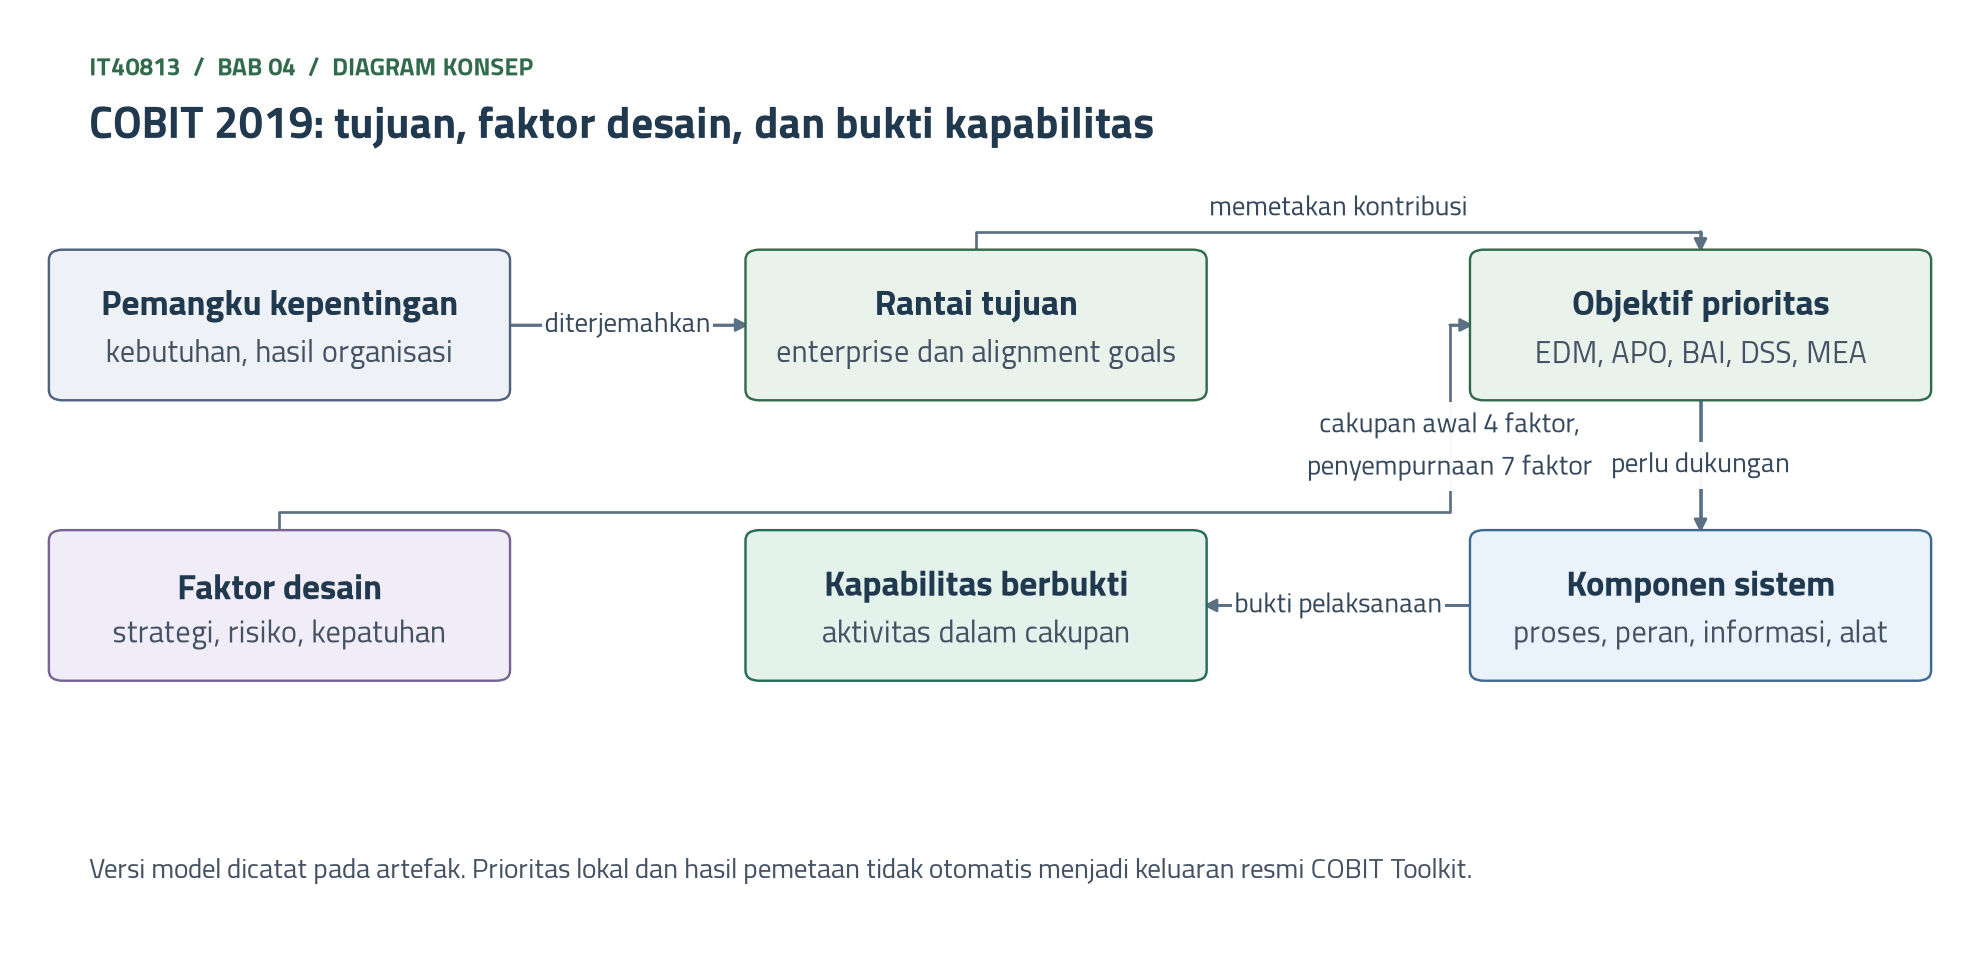
\includegraphics[width=\textwidth]{../figures/ch04-diagram-konsep.png}
  \caption{COBIT 2019: tujuan, faktor desain, dan bukti kapabilitas}
  \label{fig:ch04-ilustrasi-bab}
\end{figure}
}{}

\section{COBIT 2019 sebagai Kerangka Tata Kelola}

COBIT 2019 adalah kerangka tata kelola dan manajemen informasi serta teknologi dari ISACA.
Kerangka ini memuat prinsip, komponen, model inti berisi 40 objektif pada lima domain, serta
panduan merancang sistem tata kelola \cite{c04-baru,c04-halaman}. Cara kerjanya: organisasi
memakai konteksnya untuk memilih bagian model yang paling penting, lalu menilai pelaksanaan
bagian itu. Isi COBIT bersifat umum dan perlu disesuaikan \cite{c04-sistematis}.
Tabel~\ref{tab:ch04-publikasi} memperlihatkan empat publikasi inti dan pertanyaan yang
dijawab masing-masing \cite{cobit2019-intro,c04-gmo,cobit2019-design,c04-implementasi}. Dua
publikasi desain dan implementasi sudah menyatakan arahnya pada judul: merancang serta
menerapkan solusi, bukan menyalin isi model.

\begin{table}[!htb]
  \centering\small
  \caption{Empat publikasi inti COBIT 2019}\label{tab:ch04-publikasi}
  \begin{tabularx}{\textwidth}{|>{\raggedright\arraybackslash}p{0.36\textwidth}|>{\raggedright\arraybackslash}X|>{\raggedright\arraybackslash}p{0.17\textwidth}|}
    \hline
    \textbf{Publikasi} & \textbf{Pertanyaan yang dijawab} & \textbf{Seksi bab ini} \\ \hline
    Framework: Introduction and Methodology & Apa konsep dan prinsip kerangka ini? & Prinsip,
    komponen \\ \hline
    Framework: Governance and Management Objectives & Apa isi tiap objektif, praktik, dan
    aktivitasnya? & Model inti, kapabilitas \\ \hline
    Design Guide & Bagaimana merancang sistem sesuai konteks organisasi? & Faktor desain, rantai
    tujuan \\ \hline
    Implementation Guide & Bagaimana menerapkan dan mengoptimalkan rancangan itu? & Dibahas lagi
    pada C4 \\ \hline
  \end{tabularx}
\end{table}

Cara berpikirnya mirip bengkel mobil. Katalog bengkel memuat ratusan suku cadang. Pemilik mobil
tidak mengganti semuanya. Montir mendengar keluhan, memeriksa mobil, lalu memilih bagian yang
perlu diperbaiki. Katalog membantu menyebut nama bagian, tetapi katalog bukan rencana perbaikan.

Dua contoh kasus nyata:
\begin{enumerate}
  \item Kadam menelusuri satu tujuan organisasi tentang kelangsungan layanan. Empat objektif
  yang dipilih memuat 25 praktik dan 140 aktivitas \cite{c04-kontinuitas}. Rata-ratanya 35
  aktivitas per objektif. Misalkan rata-rata itu berlaku untuk seluruh model, sehingga 40
  objektif memuat sekitar 1.400 aktivitas. Ini perkiraan kasar, bukan hitungan resmi. Bila satu
  aktivitas diperiksa 30 menit, penilaian menyeluruh menghabiskan 700 jam atau 87,5 hari kerja
  satu orang. Empat objektif hanya memerlukan 70 jam atau 8,75 hari kerja.
  \item Bab 1 sudah menghitung bahwa 52 staf TI Medikara yang dibagi ke 40 objektif hanya
  menghasilkan 1,3 orang per objektif. Bila dibagi ke 6 objektif prioritas, angkanya sekitar 8,7
  orang. Hitungan ini kasar, sebab staf tidak dibagi rata, tetapi cukup untuk menunjukkan bahwa
  lingkup adalah keputusan, bukan urusan administrasi.
\end{enumerate}

Dua hal pada COBIT sering tertukar: sertifikat seseorang dan kapabilitas organisasi. Pembagiannya
begini. Sertifikat pelatihan menunjukkan pengetahuan seseorang. Kapabilitas menunjukkan cara
proses organisasi berjalan dan buktinya. Misalkan 4 dari 52 staf TI Medikara lulus ujian COBIT,
atau sekitar 7,7 persen. Angka itu tidak menjawab apakah 120 akun vendor sudah ditinjau. Organisasi
tidak dapat menyatakan seluruh risikonya terkendali hanya karena beberapa pegawai lulus ujian.

\begin{kasus}[title={Kasus Medikara Health: Dari Perintah ke Tiga Pertanyaan}]
Misalkan kepala TI mengembalikan perintah ``Terapkan COBIT'' kepada komite dengan tiga pertanyaan.
Masalah layanan mana yang paling merugikan? Siapa pemilik tiap masalah? Bukti apa yang akan diterima
komite? Misalkan pula konsultan mengajukan penawaran Rp600 juta untuk menilai 40 objektif.

Keputusan mempersempit lingkup punya dua konsekuensi. Pertama, penawaran Rp600 juta melewati batas
komite Rp400 juta pada Bab 2, sehingga keputusannya naik ke direksi. Direksi akan bertanya apa yang
dibeli dengan uang itu. Kedua, bila biaya mengikuti jumlah objektif, 6 objektif setara 15 persen
lingkup atau sekitar Rp90 juta. Angka itu berada di bawah batas Rp100 juta untuk kepala TI, dengan
masukan pemilik layanan. Asumsi biaya sebanding ini kasar, tetapi cukup untuk membuka diskusi tentang
apa yang dikerjakan lebih dahulu.
\end{kasus}

\section{Prinsip dan Komponen Sistem Tata Kelola}

\subsection*{Enam prinsip sistem dan tiga prinsip kerangka}

COBIT 2019 membedakan prinsip sistem tata kelola dan prinsip kerangkanya. Prinsip sistem menjelaskan
ciri sistem yang dibangun organisasi. Jumlahnya enam, naik dari lima pada COBIT 5
\cite{c04-perbandingan}. Sistem menekankan nilai bagi pemangku kepentingan, pendekatan menyeluruh,
sifat dinamis, pemisahan tata kelola dan manajemen, penyesuaian dengan kebutuhan organisasi, serta
cakupan seluruh fungsi organisasi \cite{c04-prinsip}. Prinsip kerangka menjelaskan ciri COBIT sebagai
alat: model konseptual, keterbukaan dan keluwesan, serta keselarasan dengan standar, kerangka, dan
regulasi utama \cite{c04-perbandingan}. Tabel~\ref{tab:ch04-prinsip} menerjemahkan enam prinsip sistem
ke keadaan Medikara. Kolom terakhir adalah pengandaian untuk pembelajaran.

\begin{table}[!htb]
  \centering\small
  \caption{Enam prinsip sistem tata kelola pada Medikara}\label{tab:ch04-prinsip}
  \begin{tabularx}{\textwidth}{|>{\raggedright\arraybackslash}p{0.27\textwidth}|>{\raggedright\arraybackslash}X|>{\raggedright\arraybackslash}X|}
    \hline
    \textbf{Prinsip} & \textbf{Maknanya} & \textbf{Contoh pada Medikara} \\ \hline
    Nilai bagi pemangku kepentingan & Sistem memenuhi kebutuhan dan menghasilkan nilai dari informasi
    serta teknologi & Ukuran utama adalah kerahasiaan data dan waktu tunggu, bukan jumlah prosedur \\ \hline
    Pendekatan menyeluruh & Beberapa komponen bekerja bersama & AC-01 memerlukan proses, daftar akun,
    pemilik, dan alat \\ \hline
    Sistem yang dinamis & Rancangan ditinjau ketika faktor desain berubah & Akuisisi fasilitas baru
    memicu penilaian ulang \\ \hline
    Tata kelola berbeda dari manajemen & Kegiatan dan strukturnya berbeda & Komite 9 anggota menilai
    arah; kepala TI menjalankan rencana \\ \hline
    Disesuaikan dengan kebutuhan & Kebutuhan organisasi membentuk rancangan & Medikara+ buatan vendor
    menaikkan perhatian pada vendor \\ \hline
    Mencakup seluruh fungsi & Semua fungsi, teknologi, dan informasi yang dipakai organisasi & Cakupan
    36 fasilitas, bukan hanya divisi TI pusat \\ \hline
  \end{tabularx}
\end{table}

\subsection*{Tujuh komponen}

Tujuh komponen sistem ialah proses; struktur organisasi; prinsip, kebijakan, dan prosedur; informasi;
budaya, etika, dan perilaku; orang, keterampilan, dan kompetensi; serta layanan, infrastruktur, dan
aplikasi \cite{c04-sistematis}. Istilah komponen menggantikan \textit{enabler} pada COBIT 5
\cite{c04-baru}. Perbaikan proses membutuhkan komponen lain agar berjalan. Prosedur peninjauan akses
tanpa pemilik, daftar akun, dan keterampilan pemeriksa akan sulit menghasilkan kontrol yang efektif.

Sistem perpustakaan membutuhkan aturan peminjaman, petugas, katalog, perangkat, kebiasaan
mengembalikan, dan informasi tunggakan. Menulis prosedur saja tidak membuat buku kembali ke rak.

Dua contoh penerapannya:
\begin{enumerate}
  \item Misalkan kontrol AC-01 harus meninjau 120 akun vendor, tetapi daftar yang diterima peninjau
  hanya memuat 108 akun. Sebanyak 12 akun, atau 10 persen, luput dari peninjauan. Prosedurnya tertulis
  dan peninjaunya ada. Yang lemah adalah komponen informasi, sehingga menambah prosedur tidak menutup
  celah itu.
  \item Misalkan satu rumah sakit memiliki prosedur berbeda dari empat rumah sakit lain karena SIMRS
  hasil akuisisinya berbeda. SIMRS adalah Sistem Informasi Manajemen Rumah Sakit. Penyesuaian lokal perlu
  dijelaskan agar tetap memenuhi tujuan bersama, bukan dinilai hanya dari kesamaan format.
\end{enumerate}

Tabel~\ref{tab:ch04-komponen} merangkum komponen dan bukti untuk peninjauan akses. Tabel ini dipakai
lagi saat menilai kapabilitas, sebab satu komponen yang kosong dapat menjelaskan mengapa proses gagal.

\begin{table}[!htb]
  \centering\small
  \caption{Komponen dan bukti untuk peninjauan akses AC-01}\label{tab:ch04-komponen}
  \begin{tabularx}{\textwidth}{|>{\raggedright\arraybackslash}p{0.27\textwidth}|>{\raggedright\arraybackslash}X|>{\raggedright\arraybackslash}X|}
    \hline
    \textbf{Komponen} & \textbf{Penerapan AC-01} & \textbf{Bukti} \\ \hline
    Proses & Tarik daftar, tandai, cabut, catat & Catatan peninjauan bulanan \\ \hline
    Struktur organisasi & Pengelola vendor, pemilik layanan, dan jalur eskalasi & Mandat dan
    daftar peran \\ \hline
    Prinsip, kebijakan, dan prosedur & Akun per orang dan batas waktu pencabutan & Kebijakan akses
    yang disahkan \\ \hline
    Informasi & Populasi akun dan tanggal berakhir penugasan & Daftar 120 akun dan daftar
    penugasan \\ \hline
    Budaya, etika, dan perilaku & Peninjau berani mencabut akses milik vendor penting & Tindak lanjut
    atas keberatan vendor \\ \hline
    Orang, keterampilan, dan kompetensi & Peninjau memahami peran akses & Catatan pelatihan dan
    hasil uji sampel \\ \hline
    Layanan, infrastruktur, dan aplikasi & Alat pencatatan serta pencabutan & Rekam perubahan
    akses \\ \hline
  \end{tabularx}
\end{table}

Dua hal pada sistem ini sering tertukar: tata kelola dan manajemen. Pembagiannya begini. Tata kelola
menilai pilihan, memberi arah, dan memantau apakah arah masih benar. Manajemen merencanakan, membangun,
menjalankan, dan memantau pekerjaan. Bab 2 sudah membahas pembagian ini lewat komite 9 anggota dengan
kuorum 6 orang. Komite tidak mencabut 24 akun vendor. Komite memastikan ada pemilik dan melihat hasil
peninjauan. Pertanyaan kemudian muncul: bagaimana pembagian itu terlihat pada model COBIT?

\section{Model Inti: 40 Objektif dalam Lima Domain}

Model inti berisi 40 objektif pada lima domain \cite{c04-baru}. Evaluate, Direct and Monitor (EDM) memuat
objektif tata kelola. Align, Plan and Organize (APO), Build, Acquire and Implement (BAI), Deliver,
Service and Support (DSS), serta Monitor, Evaluate and Assess (MEA) memuat objektif manajemen. Objektif
menjelaskan hasil yang perlu dicapai. Tiap objektif diuraikan menjadi praktik dan aktivitas, dan komponen
lain membantu mewujudkannya \cite{c04-kontinuitas,c04-sistematis}. Gambar~\ref{fig:ch04-model-inti}
memperlihatkan susunannya beserta enam objektif awal pengandaian Medikara yang dibahas pada seksi
berikutnya.

\begin{figure}[!htb]
  \centering
  \begin{tikzpicture}[
  kotak/.style={draw,rounded corners,align=center,text width=2.3cm,
    minimum height=1.6cm,font=\scriptsize,fill=blue!8},
  induk/.style={draw,rounded corners,align=center,text width=11.1cm,
    minimum height=0.95cm,font=\scriptsize,fill=praditagreen!15},
  pilih/.style={draw,rounded corners,align=center,text width=2.3cm,
    minimum height=0.95cm,font=\scriptsize,fill=orange!12},
  panah/.style={-{Stealth[length=2mm]},thick}
]
  \node[induk] (edm) at (4.35,2.35)
    {\textbf{EDM: 5 objektif tata kelola}\\
    {\tiny\mdseries mengevaluasi, mengarahkan, dan memantau}};
  \node[kotak] (apo) at (0,0)
    {\textbf{APO}\\14 objektif\\{\tiny\mdseries menyelaraskan dan merencanakan}};
  \node[kotak] (bai) at (2.9,0)
    {\textbf{BAI}\\11 objektif\\{\tiny\mdseries membangun dan memperoleh}};
  \node[kotak] (dss) at (5.8,0)
    {\textbf{DSS}\\6 objektif\\{\tiny\mdseries menjalankan dan mendukung}};
  \node[kotak] (mea) at (8.7,0)
    {\textbf{MEA}\\4 objektif\\{\tiny\mdseries memantau dan menilai}};
  \draw[panah] (apo) -- (bai);
  \draw[panah] (bai) -- (dss);
  \draw[panah] (dss) -- (mea);
  \draw[panah] (apo.north |- edm.south) -- node[right,font=\tiny] {arah} (apo.north);
  \draw[panah] (mea.north) -- node[left,font=\tiny] {laporan} (mea.north |- edm.south);
  \node[pilih] (p1) at (0,-1.5) {APO10, APO12, APO13, APO14};
  \node[pilih,fill=gray!35] (p2) at (2.9,-1.5) {BAI06 sebagai dependensi};
  \node[pilih] (p3) at (5.8,-1.5) {DSS05};
  \node[pilih] (p4) at (8.7,-1.5) {MEA03};
  \draw[thick,densely dashed] (apo) -- (p1);
  \draw[thick,densely dashed] (bai) -- (p2);
  \draw[thick,densely dashed] (dss) -- (p3);
  \draw[thick,densely dashed] (mea) -- (p4);
  \node[font=\scriptsize,align=center] at (4.35,-2.4)
    {5 + 14 + 11 + 6 + 4 = 40 objektif. Baris bawah: enam objektif awal pengandaian Medikara.};
\end{tikzpicture}

  \caption{Lima domain model inti COBIT 2019 dan enam objektif awal pengandaian Medikara}
  \label{fig:ch04-model-inti}
\end{figure}

Jumlah objektif pada masing-masing domain adalah 5, 14, 11, 6, dan 4. Pengenal tertinggi pada sumber yang
terbaca cocok dengan susunan itu, yaitu EDM05, APO14, BAI11, DSS06, dan MEA04, dan jumlahnya 40
\cite{c04-strategi,c04-perbandingan,c04-kapabilitas}. Katalog pada berkas sumber mencantumkan seluruh
pengenal. Nama 31 objektif sudah dicocokkan ke artikel yang terbaca. Sembilan sisanya ditandai
``perlu dicocokkan'' dan tim memeriksanya ke publikasi resmi sebelum memakainya. Katalog membantu orientasi,
sedangkan penilaian rinci tetap memerlukan aktivitas pada publikasi resmi. Tabel~\ref{tab:ch04-domain}
merangkum lima domain dengan contoh nama objektif yang sudah dicocokkan
\cite{c04-kapabilitas,c04-strategi,c04-perbandingan}.

\begin{table}[!htb]
  \centering\small
  \caption{Lima domain model inti COBIT 2019}\label{tab:ch04-domain}
  \begin{tabularx}{\textwidth}{|>{\raggedright\arraybackslash}p{0.13\textwidth}|>{\raggedright\arraybackslash}p{0.27\textwidth}|>{\raggedright\arraybackslash}X|}
    \hline
    \textbf{Domain} & \textbf{Fokus} & \textbf{Contoh objektif} \\ \hline
    EDM, 5 & Arah serta pengawasan & EDM03 \textit{Ensured risk optimization} \\ \hline
    APO, 14 & Perencanaan serta pengorganisasian & APO10 \textit{Managed vendors}; APO12
    \textit{Managed risk}; APO13 \textit{Managed security}; APO14 \textit{Managed data} \\ \hline
    BAI, 11 & Perolehan serta perubahan solusi & BAI06 \textit{Managed IT changes}; BAI11
    \textit{Managed projects} \\ \hline
    DSS, 6 & Operasi serta layanan & DSS04 \textit{Managed continuity}; DSS05 \textit{Managed
    security services} \\ \hline
    MEA, 4 & Pemantauan serta penilaian & MEA03 \textit{Managed compliance with external requirements};
    MEA04 \textit{Managed assurance} \\ \hline
  \end{tabularx}
\end{table}

Struktur di bawah objektif menjelaskan mengapa model ini terasa besar. DSS04, misalnya, memiliki 8 praktik
\cite{c04-sistematis}. Tiap aktivitas pada komponen proses dikaitkan dengan satu tingkat kapabilitas
\cite{c04-baru}. Satu objektif bukan satu baris pemeriksaan, melainkan sekumpulan pekerjaan yang dapat
diuji satu per satu.

Risiko vendor melintasi domain. Pengelolaan hubungan vendor, keamanan, data, perubahan, dan asurans saling
terkait. Memilih satu objektif prioritas tidak berarti objektif lain tidak diperlukan. Pilihan menunjukkan
fokus penilaian dan perbaikan pada tahap tertentu.

Peta layanan rumah sakit membagi pekerjaan ke rawat jalan, laboratorium, farmasi, dan unit lain. Pembagian
membantu menemukan penanggung jawab, tetapi perjalanan satu pasien tetap melewati beberapa unit.

Dua contoh penerapannya:
\begin{enumerate}
  \item Misalkan temuan 6 dari 30 akun vendor mengarah pada APO10 untuk hubungan vendor dan DSS05 untuk
  layanan keamanan. Tim menilai keduanya bersama bukti perintah akses. Bila hanya DSS05 yang dinilai,
  12 akun yang tidak tercatat tetap luput, sebab daftar akun itu bersumber dari pengelolaan vendor.
  \item Misalkan pembaruan aplikasi di rumah sakit Bogor mengubah format nomor rekam medis, sehingga
  2.400 dari 96.000 data pasien, atau 2,5 persen, tidak cocok dengan data pusat. BAI06 tentang perubahan
  dan APO14 tentang data membantu menelusuri keputusan serta kontrol yang terkait. Satu kejadian
  menyentuh dua domain.
\end{enumerate}

\section{Faktor Desain dan Focus Area}

\subsection*{Sebelas faktor desain}

Sebelas faktor desain membentuk pilihan objektif dan target kapabilitas. Faktor tersebut mencakup
strategi, tujuan organisasi, profil risiko, isu terkait TI, ancaman, kebutuhan kepatuhan, peran TI, model
penyediaan, metode implementasi, strategi adopsi teknologi, dan ukuran organisasi
\cite{cobit2019-design,c04-perbandingan,c04-operasional}. Empat faktor pertama menetapkan cakupan awal, lalu
faktor lain memperhalus prioritas \cite{c04-kapabilitas,c04-perbandingan}. \textit{Toolkit} COBIT
menghasilkan skor tiap objektif untuk cakupan awal, cakupan yang disempurnakan, dan cakupan akhir. Cakupan
akhir lahir setelah konflik diselesaikan dan rancangan dituntaskan \cite{c04-perbandingan}.
Gambar~\ref{fig:ch04-cakupan-desain} memperlihatkan urutan itu.

\begin{figure}[!htb]
  \centering
  \begin{tikzpicture}[
  kotak/.style={draw,rounded corners,align=center,text width=2.5cm,
    minimum height=2.3cm,font=\scriptsize,fill=blue!8},
  panah/.style={-{Stealth[length=2mm]},thick}
]
  \node[kotak,fill=praditagreen!15] (a) at (0,0)
    {\textbf{Konteks}\\strategi dan keadaan organisasi\\
    {\tiny\mdseries sumber: dokumen dan wawancara}};
  \node[kotak] (b) at (3.0,0)
    {\textbf{Cakupan awal}\\4 faktor\\
    {\tiny\mdseries strategi, tujuan organisasi, profil risiko, isu TI}};
  \node[kotak,fill=orange!12] (c) at (6.0,0)
    {\textbf{Penyempurnaan}\\7 faktor\\
    {\tiny\mdseries ancaman, kepatuhan, peran TI, model penyediaan, metode implementasi,
    adopsi teknologi, ukuran}};
  \node[kotak,fill=green!10] (d) at (9.0,0)
    {\textbf{Kesimpulan}\\konflik diselesaikan\\
    {\tiny\mdseries objektif prioritas dan target kapabilitas}};
  \draw[panah] (a) -- (b);
  \draw[panah] (b) -- (c);
  \draw[panah] (c) -- (d);
  \draw[panah] (d.south) -- ++(0,-0.4) -| node[pos=0.25,below,font=\scriptsize]
    {faktor berubah: rancangan dinilai ulang} (a.south);
\end{tikzpicture}

  \caption{Faktor desain dipakai bertahap untuk menyusun cakupan sistem tata kelola}
  \label{fig:ch04-cakupan-desain}
\end{figure}

Rancangan sistem air untuk rumah satu lantai berbeda dari rancangan jaringan air kompleks rumah sakit.
Tujuannya sama-sama menyediakan air, tetapi ukuran, kebutuhan layanan, risiko, dan sumber pasokan menentukan
bagian yang perlu diperkuat.

Tabel~\ref{tab:ch04-faktor} merangkum sebelas faktor dengan kategori penilaian. Kategori diambil dari
lembar \textit{toolkit} yang dilaporkan studi rumah sakit di Denpasar \cite{c04-denpasar}. Tim memeriksa
ulang rumusannya pada versi \textit{toolkit} yang dipakai.

\begin{table}[!htb]
  \centering\footnotesize
  \caption{Sebelas faktor desain, kategori penilaian, dan bukti}\label{tab:ch04-faktor}
  \begin{tabularx}{\textwidth}{|>{\raggedright\arraybackslash}p{0.23\textwidth}|>{\raggedright\arraybackslash}X|>{\raggedright\arraybackslash}p{0.27\textwidth}|}
    \hline
    \textbf{Faktor} & \textbf{Kategori penilaian} & \textbf{Bukti contoh} \\ \hline
    Strategi organisasi & \textit{Growth/acquisition, innovation/differentiation, cost leadership, client
    service/stability} & Dokumen strategi \\ \hline
    Tujuan organisasi & EG01 sampai EG13, nilai 1 sampai 5 & Rencana kerja direksi \\ \hline
    Profil risiko & Kategori skenario risiko, dampak 1 sampai 5 & Register risiko, insiden \\ \hline
    Isu terkait TI & Daftar isu, tingkat 1 sampai 3 & Temuan audit, tiket berulang \\ \hline
    Ancaman & \textit{High, normal} & Analisis ancaman, paparan \\ \hline
    Kebutuhan kepatuhan & \textit{High, normal, low} & Register kewajiban C1 \\ \hline
    Peran TI & \textit{Support, factory, turnaround, strategic} & Peta layanan dan dampak \\ \hline
    Model penyediaan & \textit{Outsourcing, cloud, insourced} & Kontrak, daftar layanan \\ \hline
    Metode implementasi & \textit{Agile}, DevOps, \textit{traditional} & Rencana kerja, data rilis \\ \hline
    Strategi adopsi teknologi & \textit{First mover, follower, slow adopter} & Peta jalan teknologi \\ \hline
    Ukuran organisasi & Besar atau kecil dan menengah & Data karyawan \\ \hline
  \end{tabularx}
\end{table}

Dua contoh penerapannya:
\begin{enumerate}
  \item Studi di Denpasar mencatat rumah sakit dengan 170 karyawan sebagai organisasi kecil dan menengah,
  dengan rentang 50 sampai 250 karyawan, dan model penyediaan 75 persen \textit{outsourcing}
  \cite{c04-denpasar}. Medikara memiliki sekitar 4.800 karyawan, atau 19,2 kali batas atas itu. Klinik mitra
  60 karyawan pada Bab 3 masuk rentang tersebut. Satu jaringan layanan dapat berhadapan dengan dua kategori
  ukuran pada rancangan yang berbeda.
  \item Misalkan Medikara mengakuisisi dua fasilitas baru dalam skenario latihan, sehingga 36 fasilitas menjadi
  38, atau naik sekitar 5,6 persen. Isu integrasi dan akses lintas unit perlu dinilai kembali, meskipun tujuan
  layanan tidak berubah. Inilah arti prinsip sistem yang dinamis.
\end{enumerate}

Dua rumah sakit di Indonesia memperlihatkan pengaruh konteks. Studi di Denpasar menghasilkan lima objektif:
APO12, APO13, BAI06, DSS04, dan DSS05 \cite{c04-denpasar}. Studi di Kediri, pada Rumah Sakit Wilujeng,
menghasilkan tiga: DSS05, APO07, dan APO12 \cite{c04-wilujeng}. Keduanya memiliki 2 objektif yang sama, yaitu
APO12 dan DSS05, dari 6 objektif berbeda. Studi pertama menyebut 11 faktor, sedangkan studi kedua menyebut 10
faktor. Pembaca perlu mencatat perbedaan metode itu sebelum menyimpulkan bahwa perbedaan hasil hanya berasal
dari konteks.

Penilaian faktor harus memiliki dasar. Kategori ketergantungan vendor ditopang daftar layanan dan kontrak.
Kategori ancaman ditopang insiden serta paparan. Bila data belum ada, tim mencatat asumsi dan menguji
pengaruhnya pada prioritas. Penilaian ulang diperlukan ketika strategi, vendor, atau lingkungan berubah.
Tabel~\ref{tab:ch04-faktor-medikara} mengisi faktor untuk Medikara dan membedakan fakta kasus dari
pengandaian. Rumusan isu dan risiko berbahasa Inggris mengikuti daftar pada studi Denpasar.

\begin{table}[!htb]
  \centering\footnotesize
  \caption{Sebelas faktor desain pada Medikara: fakta kasus dan pengandaian}\label{tab:ch04-faktor-medikara}
  \begin{tabularx}{\textwidth}{|>{\raggedright\arraybackslash}p{0.22\textwidth}|>{\raggedright\arraybackslash}X|>{\raggedright\arraybackslash}p{0.17\textwidth}|}
    \hline
    \textbf{Faktor} & \textbf{Nilai pada Medikara} & \textbf{Status} \\ \hline
    Strategi organisasi & Layanan terintegrasi lintas fasilitas: \textit{client service/stability} tertinggi
    & Pengandaian dari strategi kasus \\ \hline
    Tujuan organisasi & EG06 kelangsungan layanan, EG03 kepatuhan, EG12 transformasi digital & Pengandaian \\
    \hline
    Profil risiko & \textit{Third-party/supplier incidents, unauthorized actions}; R-01 & Insiden 2025 fakta;
    rincian pengandaian \\ \hline
    Isu terkait TI & Temuan audit berulang, masalah layanan dari vendor, integrasi data, biaya integrasi & Fakta
    kasus \\ \hline
    Ancaman & \textit{High} 75 persen, \textit{normal} 25 persen & Pengandaian \\ \hline
    Kebutuhan kepatuhan & \textit{High}: register K-01 sampai K-16 pada 36 fasilitas & Register C1 \\ \hline
    Peran TI & \textit{Factory} dan \textit{turnaround}: SIMRS menopang layanan, sedang dimodernisasi & Pengandaian
    \\ \hline
    Model penyediaan & Medikara+ dan dukungan vendor; SIMRS \textit{on-premise} di tiap rumah sakit & Fakta kasus \\
    \hline
    Metode implementasi & \textit{Traditional} 70 persen, \textit{agile} 25 persen, DevOps 5 persen &
    Pengandaian \\ \hline
    Strategi adopsi teknologi & \textit{Follower}: modernisasi \textit{cloud} bertahap sampai 2030 & Pengandaian
    dari strategi kasus \\ \hline
    Ukuran organisasi & Sekitar 4.800 karyawan, 52 staf TI, tim platform 6 orang & Fakta kasus \\ \hline
  \end{tabularx}
\end{table}

\subsection*{Focus area}

Dua hal pada rancangan ini sering tertukar: faktor desain dan \textit{focus area}. Pembagiannya begini. Faktor desain
menggambarkan keadaan organisasi. \textit{Focus area} memberi perhatian pada tema tertentu dan memakai objektif serta
komponen yang relevan. ISACA menerbitkan panduan untuk DevOps, risiko informasi dan teknologi, keamanan informasi,
serta organisasi kecil dan menengah \cite{c04-halaman}. Tema bukan domain keenam dan tidak membenarkan mengabaikan
keputusan yang berpengaruh pada tujuan layanan. Kalimat terakhir ini adalah penafsiran bab ini.

Analoginya seperti klinik spesialis di dalam rumah sakit. Klinik jantung memberi perhatian khusus, tetapi tetap memakai
laboratorium, farmasi, dan rekam medis yang sama.

Dua contoh penerapannya:
\begin{enumerate}
  \item Misalkan tim platform 6 orang ingin mempercepat rilis Medikara+. Panduan DevOps relevan bagi 6 orang itu.
  Panduan yang sama tidak menjawab kewajiban peninjauan 120 akun vendor, sehingga tema ini tidak menggantikan
  objektif prioritas.
  \item Misalkan klinik mitra berkaryawan 60 orang dengan 2 staf TI ingin menerapkan COBIT. Panduan organisasi kecil
  dan menengah lebih masuk akal sebagai titik awal, sebab 2 staf tidak dapat menjalankan rancangan milik jaringan
  dengan 52 staf TI.
\end{enumerate}

\begin{pendalaman}
Gunakan \textit{toolkit} COBIT resmi bila aksesnya tersedia. Halaman COBIT di situs ISACA menautkan berkasnya
\cite{c04-halaman}. Bobot faktor mengikuti kepentingan relatif tiap objektif, dan nilainya dihitung sebagai selisih
persentase antara kondisi dasar dan kondisi organisasi \cite{c04-perbandingan}. Ubah satu faktor pada satu waktu dan
catat perubahan prioritas. Bandingkan hasil dengan alasan manual, lalu jelaskan perbedaan. Hindari memberi nama skor resmi
kepada rumus lokal. Lembar kerja pada folder sumber sengaja memisahkan data konteks, prioritas, dan bukti agar penalarannya
dapat ditinjau tanpa alat berbayar. Mahasiswa berlatar rekayasa perangkat lunak dapat membandingkan hasilnya dengan
\textit{focus area} DevOps.
\end{pendalaman}

\section{Goals Cascade dan Pemilihan Prioritas}

\textit{Goals cascade} atau rantai tujuan menghubungkan kebutuhan pemangku kepentingan, tujuan organisasi
(\textit{enterprise goal}, EG), tujuan keselarasan (\textit{alignment goal}, AG), dan objektif tata kelola serta manajemen
\cite{c04-routsis,c04-sistematis}. COBIT 2019 memuat 13 EG dan 13 AG \cite{c04-strategi,c04-transformasi}. Pemetaan membantu
menjelaskan mengapa objektif dipilih. Tiap hubungan diberi tanda primer atau sekunder \cite{c04-kontinuitas}. Hubungan pada model
resmi adalah alat bantu. Konteks organisasi tetap perlu menjelaskan pilihan akhirnya \cite{c04-kontinuitas,c04-sistematis}.

Rencana perjalanan dimulai dari tujuan dan kebutuhan peserta, lalu memilih rute serta alat transportasi. Menghitung kenyamanan
kursi sebelum menentukan tujuan tidak membantu memilih perjalanan yang tepat.

Dua contoh penerapannya:
\begin{enumerate}
  \item Kadam memulai dari EG06, yaitu \textit{business service continuity and availability}. EG06 terhubung ke AG07 sebagai
  primer, serta AG02 dan AG05 sebagai sekunder. Objektif berprioritas primer berjumlah 17, sehingga penulisnya menilai jumlah
  itu kurang praktis. Daftar dipersempit menjadi 8 objektif, lalu 4 objektif untuk fokus awal, yaitu APO09, APO10, DSS04, dan
  DSS05 \cite{c04-kontinuitas}. Dari 40 objektif, yang tersisa 10 persen. Gambar~\ref{fig:ch04-rantai-tujuan} memperlihatkan
  penyaringan itu.
  \item Rafeq dan Elangovan memakai EG06 yang sama, tetapi memilih jalur lain. Enam objektif primer untuk AG07 adalah EDM03,
  APO12, APO13, BAI10, DSS04, dan DSS05, lalu contoh mereka memilih DSS04 berdasarkan kekritisan dan relevansi
  \cite{c04-sistematis}. Titik awal yang sama dapat berakhir pada pilihan berbeda. Karena itu alasan harus tertulis.
\end{enumerate}

\begin{figure}[!htb]
  \centering
  \begin{tikzpicture}[
  kotak/.style={draw,rounded corners,align=center,text width=3.3cm,
    minimum height=1.25cm,font=\scriptsize,fill=blue!8},
  saring/.style={draw,rounded corners,align=center,text width=2.3cm,
    minimum height=1.25cm,font=\scriptsize,fill=orange!12},
  panah/.style={-{Stealth[length=2mm]},thick}
]
  \node[kotak,fill=praditagreen!15] (k) at (0,0)
    {\textbf{Kebutuhan pemangku kepentingan}\\
    {\tiny\mdseries layanan tetap berjalan saat terganggu}};
  \node[kotak] (e) at (3.95,0)
    {\textbf{Tujuan organisasi}\\EG06\\
    {\tiny\mdseries \textit{business service continuity and availability}}};
  \node[kotak] (g) at (7.9,0)
    {\textbf{Tujuan keselarasan}\\AG07 primer\\
    {\tiny\mdseries AG02 dan AG05 sekunder}};
  \draw[panah] (k) -- (e);
  \draw[panah] (e) -- (g);
  \node[saring,fill=gray!35] (s0) at (-0.5,-2.25)
    {\textbf{40}\\{\tiny\mdseries objektif model inti}};
  \node[saring] (s1) at (2.45,-2.25)
    {\textbf{17}\\{\tiny\mdseries objektif berprioritas primer}};
  \node[saring] (s2) at (5.4,-2.25)
    {\textbf{8}\\{\tiny\mdseries daftar pendek sesuai konteks}};
  \node[saring,fill=green!10] (s3) at (8.35,-2.25)
    {\textbf{4}\\{\tiny\mdseries fokus awal: 25 praktik, 140 aktivitas}};
  \draw[panah] (s0) -- (s1);
  \draw[panah] (s1) -- (s2);
  \draw[panah] (s2) -- (s3);
  \draw[panah] (g.south) -- ++(0,-0.3) -| (s0.north);
\end{tikzpicture}

  \caption{Rantai tujuan dan penyaringan objektif menurut contoh Kadam}
  \label{fig:ch04-rantai-tujuan}
\end{figure}

Rantai penalaran dimulai dari masalah yang dapat dikenali pemilik layanan. Tim merumuskan hasil organisasi, lalu kemampuan
informasi dan teknologi yang mendukungnya. Faktor desain dipakai untuk menguji apakah prioritas tersebut masuk akal terhadap
risiko serta batas sumber daya. Tabel~\ref{tab:ch04-cascade} memperlihatkan rantai untuk Medikara. Nama EG dan AG hanya ditulis
bila terbaca pada sumber. Kolom terakhir menyatakan bagian mana yang tercantum pada sumber dan bagian mana yang merupakan
penafsiran bab ini.

\begin{table}[!htb]
  \centering\footnotesize
  \caption{Contoh rantai prioritas Medikara}\label{tab:ch04-cascade}
  \begin{tabularx}{\textwidth}{|>{\raggedright\arraybackslash}p{0.2\textwidth}|>{\raggedright\arraybackslash}p{0.13\textwidth}|>{\raggedright\arraybackslash}p{0.12\textwidth}|>{\raggedright\arraybackslash}p{0.14\textwidth}|>{\raggedright\arraybackslash}X|}
    \hline
    \textbf{Kebutuhan} & \textbf{EG} & \textbf{AG} & \textbf{Objektif} & \textbf{Status pemetaan} \\ \hline
    Kerahasiaan data pasien & EG06 & AG07 & APO13; DSS05 & Tercantum pada sumber \\ \hline
    Vendor dapat dipertanggungjawabkan & EG06 & AG05 & APO10 & Tercantum pada sumber \\ \hline
    Risiko layanan terkendali & EG02 & AG02 & APO12 & Penafsiran bab ini; EG dan AG terbaca \\ \hline
    Identitas pasien konsisten & EG12 & AG08 & APO14 & Penafsiran bab ini; cocokkan ke tabel resmi \\ \hline
    Kewajiban dapat dibuktikan & EG03 & Belum ditetapkan & MEA03 & Penafsiran bab ini; AG dicari pada tabel resmi \\ \hline
  \end{tabularx}
\end{table}

Skor prioritas lokal pada latihan merupakan alat diskusi, bukan keluaran resmi \textit{toolkit} COBIT. Bobot, asumsi, dan perubahan
urutan harus ditulis. Dua objektif dengan skor sama dapat memiliki urgensi berbeda bila satu berkaitan dengan kewajiban hukum atau
keselamatan pasien. Tabel~\ref{tab:ch04-skor} memberi nilai 1 sampai 5 pada tiga pertanyaan: seberapa besar kaitannya dengan risiko
R-01 dan insiden, seberapa besar kaitannya dengan register kewajiban, dan seberapa besar kaitannya dengan strategi Satu Pasien, Satu
Rekam Medis. Semua nilai adalah pengandaian.

\begin{table}[!htb]
  \centering\small
  \caption{Skor prioritas lokal Medikara (pengandaian, nilai maksimum 15)}\label{tab:ch04-skor}
  \begin{tabularx}{\textwidth}{|>{\raggedright\arraybackslash}p{0.13\textwidth}|>{\raggedright\arraybackslash}p{0.09\textwidth}|>{\raggedright\arraybackslash}p{0.13\textwidth}|>{\raggedright\arraybackslash}p{0.11\textwidth}|>{\raggedright\arraybackslash}p{0.07\textwidth}|>{\raggedright\arraybackslash}X|}
    \hline
    \textbf{Objektif} & \textbf{Risiko} & \textbf{Kewajiban} & \textbf{Strategi} & \textbf{Total} & \textbf{Keputusan} \\ \hline
    APO10 & 5 & 4 & 3 & 12 & Masuk \\ \hline
    DSS05 & 5 & 5 & 2 & 12 & Masuk \\ \hline
    APO13 & 4 & 4 & 3 & 11 & Masuk \\ \hline
    APO14 & 3 & 3 & 5 & 11 & Masuk \\ \hline
    APO12 & 4 & 3 & 3 & 10 & Masuk \\ \hline
    MEA03 & 2 & 5 & 3 & 10 & Masuk \\ \hline
    DSS04 & 3 & 4 & 3 & 10 & Ditunda ke Bab 10 \\ \hline
    BAI06 & 3 & 2 & 4 & 9 & Dependensi \\ \hline
    APO09 & 3 & 2 & 2 & 7 & Ditunda \\ \hline
  \end{tabularx}
\end{table}

Skor memberi tiga objektif bernilai 10, sedangkan kapasitas hanya menyisakan dua tempat. Di sinilah tahap kesimpulan bekerja. Dua
pilihan lalu diambil dengan alasan. APO12 masuk karena R-01 memerlukan pemilik dan pemantauan yang sama pada semua fasilitas. MEA03
masuk karena 16 baris register kewajiban belum memiliki pemantauan bersama. DSS04 ditunda sampai analisis dampak bisnis pada Bab 10,
tetapi kewajiban 36 prosedur dan 144 uji pemulihan per tahun dari Bab 3 tetap tercatat sebagai pekerjaan berjalan.

Target kapabilitas juga berasal dari skor. Menurut Souza Neto dan rekan, panduan desain memberi contoh sebuah perusahaan manufaktur: skor
75 atau lebih memerlukan tingkat 4, skor 50 atau lebih tingkat 3, skor 25 atau lebih tingkat 2, dan sisanya tingkat 1. Ambang itu adalah
logika contoh tersebut, bukan aturan umum. Mereka juga mengkritik akibatnya: semua proses di bawah objektif berskor sama menerima satu
tingkat yang sama \cite{c04-kapabilitas}. Bab 8 mengambil keputusan target, sedangkan bab ini berhenti pada kondisi saat ini.

\begin{kasus}[title={Kasus Medikara Health: Memilih Enam Objektif Awal}]
Misalkan Medikara memilih APO10, APO12, APO13, APO14, DSS05, dan MEA03 sebagai enam objektif awal. Pilihan tersebut ditopang
ketergantungan vendor, insiden 2025, temuan kontrol akses, data yang tersebar, dan kewajiban yang perlu dibuktikan. BAI06 tetap dicatat
sebagai dependensi perubahan. Daftar ini merupakan hasil pengandaian untuk diskusi. Tim harus mengubahnya bila konteks dan bukti
menunjukkan prioritas berbeda.

Pilihan ini punya dua konsekuensi yang dapat dihitung. Pertama, bila bobot kewajiban digandakan, DSS05 menjadi 17, APO10 menjadi 16, APO13
dan MEA03 menjadi 15, APO14 dan DSS04 menjadi 14, serta APO12 menjadi 13. APO12 turun ke urutan ketujuh dan DSS04 masuk enam besar.
Urutan bergantung pada bobot, sehingga bobot perlu disetujui komite, bukan dipilih analis sendirian. Kedua, dengan rata-rata 35 aktivitas
per objektif, enam objektif setara 210 aktivitas atau 105 jam pemeriksaan. Hitungan itu berbeda jauh dari 700 jam untuk 40 objektif.
\end{kasus}

\section{Penilaian Kapabilitas Berdasarkan Bukti}

\subsection*{Tingkat kapabilitas 0 sampai 5}

COBIT 2019 menggunakan pendekatan kapabilitas proses yang mengacu pada Capability Maturity Model Integration (CMMI), dengan tingkat 0 sampai
5 \cite{c04-perbandingan}. Aktivitas memiliki hubungan dengan tingkat kapabilitas, sehingga penilaian perlu memeriksa aktivitas yang berlaku
pada objektif tersebut \cite{c04-baru}. Skala COBIT 5 tidak boleh dipindahkan begitu saja ke COBIT 2019, sebab COBIT 5 memakai skala berbasis
ISO/IEC 33000, standar dari International Organization for Standardization (ISO) dan International Electrotechnical Commission (IEC)
\cite{c04-perbandingan}.

Tingkat 0 menunjukkan pendekatan belum memadai. Tingkat 1 masih awal dan belum lengkap. Tingkat 2 mencapai tujuan melalui aktivitas dasar yang
lengkap. Tingkat 3 menggunakan cara kerja dan aset organisasi. Tingkat 4 mengukur kinerja secara kuantitatif. Tingkat 5 memakai pengukuran untuk
perbaikan berkelanjutan \cite{c04-kapabilitas}. Gambar~\ref{fig:ch04-tangga-kapabilitas} menyusunnya sebagai tangga. Ini ringkasan orientasi,
bukan rubrik penetapan formal.

\begin{figure}[!htb]
  \centering
  \begin{tikzpicture}[
  anak/.style={draw,rounded corners,align=center,text width=1.68cm,
    minimum height=1.05cm,font=\scriptsize,fill=blue!8},
  panah/.style={-{Stealth[length=2mm]},thick}
]
  \node[anak,fill=gray!35] (t0) at (0,0)
    {\textbf{0}\\{\tiny\mdseries belum memadai}};
  \node[anak] (t1) at (1.95,0.8)
    {\textbf{1}\\{\tiny\mdseries aktivitas belum lengkap}};
  \node[anak] (t2) at (3.9,1.6)
    {\textbf{2}\\{\tiny\mdseries aktivitas dasar lengkap}};
  \node[anak,fill=orange!12] (t3) at (5.85,2.4)
    {\textbf{3}\\{\tiny\mdseries memakai aset organisasi}};
  \node[anak] (t4) at (7.8,3.2)
    {\textbf{4}\\{\tiny\mdseries kinerja diukur kuantitatif}};
  \node[anak,fill=green!10] (t5) at (9.75,4.0)
    {\textbf{5}\\{\tiny\mdseries perbaikan berkelanjutan}};
  \draw[panah] (t0.north) |- (t1.west);
  \draw[panah] (t1.north) |- (t2.west);
  \draw[panah] (t2.north) |- (t3.west);
  \draw[panah] (t3.north) |- (t4.west);
  \draw[panah] (t4.north) |- (t5.west);
  \node[font=\scriptsize,align=left,text width=6.6cm] at (6.75,0.3)
    {Tiap tingkat diperiksa lewat aktivitas dan buktinya pada cakupan yang tertulis.
    Tingkat yang lebih tinggi tidak otomatis menjadi target semua objektif.};
\end{tikzpicture}

  \caption{Tingkat kapabilitas proses COBIT 2019 sebagai tangga}
  \label{fig:ch04-tangga-kapabilitas}
\end{figure}

Satu foto dapur yang bersih tidak membuktikan kebersihan terjaga sepanjang bulan. Pemeriksa perlu melihat jadwal, catatan, contoh hari berbeda,
serta tindak lanjut penyimpangan.

Dua contoh penerapannya:
\begin{enumerate}
  \item Misalkan 8 dari 10 perubahan memiliki persetujuan, tetapi tidak ada analisis dampak pada dua perubahan darurat. Tim mencatat celah itu
  sebelum menerima klaim proses perubahan tingkat 3. Dua tiket yang gagal adalah jenis perubahan yang paling berisiko, sehingga 80 persen
  tidak mewakili keadaan terburuk.
  \item Misalkan AC-01 memiliki prosedur korporat, tetapi bukti peninjauan baru tersedia pada satu dari lima rumah sakit, atau 20 persen. Lingkup
  bukti belum mendukung klaim penerapan menyeluruh. Keputusan yang wajar adalah membatasi klaim pada satu lokasi itu.
\end{enumerate}

\subsection*{Peringkat capaian dan aturan penetapan}

Pertanyaan kemudian muncul: kapan satu tingkat dinyatakan tercapai? Tabel~\ref{tab:ch04-peringkat} memuat empat peringkat capaian yang lazim dipakai.
Souza Neto dan rekan menyebut peringkat itu serupa dengan ISO/IEC 33004 \cite{c04-kapabilitas}, sedangkan studi Denpasar merujuknya ke ISACA
\cite{c04-denpasar}. Batas pada kedua sumber sedikit berbeda, yaitu 85 persen dan 84 persen sebagai batas atas \textit{largely}.

\begin{table}[!htb]
  \centering\small
  \caption{Peringkat capaian menurut dua sumber}\label{tab:ch04-peringkat}
  \begin{tabularx}{\textwidth}{|>{\raggedright\arraybackslash}p{0.22\textwidth}|>{\raggedright\arraybackslash}X|>{\raggedright\arraybackslash}X|}
    \hline
    \textbf{Peringkat} & \textbf{Souza Neto dan rekan} & \textbf{Studi Denpasar} \\ \hline
    N, \textit{not achieved} & Kurang dari 15 persen & 0 sampai 14 persen \\ \hline
    P, \textit{partially achieved} & 15 sampai 50 persen & 15 sampai 49 persen \\ \hline
    L, \textit{largely achieved} & 50 sampai 85 persen & 50 sampai 84 persen \\ \hline
    F, \textit{fully achieved} & Lebih dari 85 persen & 85 sampai 100 persen \\ \hline
  \end{tabularx}
\end{table}

Aturan penetapan perlu ditulis, sebab hasilnya bergantung pada aturan itu. Dua studi rumah sakit hanya menyatakan satu tingkat tercapai bila capaiannya
penuh, dan studi Denpasar menuliskannya sebagai 85 persen atau lebih. Bila belum, penilaian berhenti \cite{c04-denpasar,c04-wilujeng}. Usulan Souza Neto dan
rekan untuk menetapkan target menerima peringkat L atau F pada tiap aktivitas \cite{c04-kapabilitas}. Keduanya menjawab pertanyaan berbeda, tetapi memperlihatkan
bahwa angka yang sama dapat dibaca berbeda. Rumusan resmi perlu dicocokkan ke publikasi ISACA sebelum dipakai dalam asesmen formal. Dua contoh di bawah
memperlihatkan akibatnya:
\begin{enumerate}
  \item Di Kediri, APO07 mencapai 100 persen pada tingkat 1 dan 80,55 persen pada tingkat 2. Peringkatnya \textit{largely}, sehingga APO07 dinyatakan tetap
  tingkat 1 \cite{c04-wilujeng}. Tanpa aturan itu, pembaca dapat keliru mengira 80,55 persen sudah dekat dengan tingkat 2 yang terpenuhi.
  \item Di Denpasar, lima responden menilai APO12 tingkat 2 dengan nilai 66, 66, 50, 50, dan 83 persen. Jumlahnya 315 dan rata-ratanya 63 persen, sehingga APO12
  dinyatakan tingkat 1 \cite{c04-denpasar}. Selisih responden tertinggi dan terendah 33 poin. Rata-rata menyembunyikan perbedaan pandangan itu.
\end{enumerate}

\subsection*{Membaca studi kapabilitas secara kritis}

Studi rumah sakit berguna sebagai contoh alur, dan layak dibaca kritis. Tabel~\ref{tab:ch04-studi} membandingkan dua studi. Penilaian kedua studi terutama bersandar
pada jawaban responden, walaupun studi Denpasar juga menyebut observasi dan wawancara. Pada Denpasar, kelima responden memberikan nilai yang sama pada dua objektif:
71 persen untuk APO13 dan 60 persen untuk BAI06. Pembaca patut bertanya apakah itu lima pengamatan atau satu pendapat yang disepakati. Naskah yang sama menyebut kelima
objektif bernilai 75 dan memerlukan tingkat 4, tetapi tabel target mencantumkan tingkat 3 untuk APO12 dan DSS04. Pembacaan ini adalah penafsiran bab ini.

\begin{table}[!htb]
  \centering\footnotesize
  \caption{Dua studi kapabilitas rumah sakit di Indonesia}\label{tab:ch04-studi}
  \begin{tabularx}{\textwidth}{|>{\raggedright\arraybackslash}p{0.2\textwidth}|>{\raggedright\arraybackslash}X|>{\raggedright\arraybackslash}X|}
    \hline
    \textbf{Aspek} & \textbf{Rumah Sakit Umum Bhakti Rahayu Denpasar \cite{c04-denpasar}} & \textbf{Rumah Sakit Wilujeng \cite{c04-wilujeng}} \\ \hline
    Faktor desain & 11 faktor, memilih objektif bernilai 75 & 10 faktor dengan Design Toolkit \\ \hline
    Objektif dan tingkat saat ini & APO12 dan DSS04 tingkat 1; APO13, BAI06, DSS05 tingkat 2 & DSS05, APO07, dan APO12 tingkat 1 \\ \hline
    Capaian yang dilaporkan & APO12 63 persen, DSS04 56 persen pada tingkat 2 & 61,5; 80,55; dan 58,33 persen pada tingkat 2 \\ \hline
    Sumber data & Kuesioner lima karyawan, observasi, wawancara & Kuesioner skala Guttman, manajer unit TI, satu responden sumber daya manusia untuk APO07 \\ \hline
    Target & APO12 dan DSS04 tingkat 3; lainnya tingkat 4 & Dibandingkan lewat analisis celah \\ \hline
    Pertanyaan pembaca & Bukti apa yang menopang jawaban kuesioner? & Apakah satu manajer dapat menilai pekerjaannya sendiri? \\ \hline
  \end{tabularx}
\end{table}

\subsection*{Potret cepat untuk capstone}

Potret cepat dalam capstone melaporkan aktivitas yang diamati, bukti yang tersedia, celah, dan tingkat indikatif dengan batas keyakinannya. Wawancara hanya satu
jenis bukti. Sampel, periode, lokasi, dan populasi perlu disebutkan. Ketiadaan bukti tidak sama dengan bukti bahwa pekerjaan tidak pernah dilakukan, tetapi klaim
kapabilitas belum dapat diterima.

Kapabilitas proses juga berbeda dari satu angka gabungan. COBIT 2019 memakai skala 0 sampai 5 untuk kapabilitas dan kematangan \cite{c04-perbandingan}. Bab ini memakai
kapabilitas per objektif prioritas. Satu angka rata-rata tidak menjelaskan apakah proses kritis gagal. Tim perlu melaporkan proses dan celahnya secara terpisah agar
perbaikan mengikuti risiko layanan. Tabel~\ref{tab:ch04-kapabilitas} merangkum bukti dan batas klaim kapabilitas.

\begin{table}[!htb]
  \centering\small
  \caption{Bukti dan batas klaim kapabilitas}\label{tab:ch04-kapabilitas}
  \begin{tabularx}{\textwidth}{|>{\raggedright\arraybackslash}p{0.22\textwidth}|>{\raggedright\arraybackslash}X|>{\raggedright\arraybackslash}X|}
    \hline
    \textbf{Klaim} & \textbf{Bukti yang diperlukan} & \textbf{Batas kesimpulan} \\ \hline
    Pekerjaan dilakukan & Contoh hasil dan pelaksana & Belum membuktikan konsistensi \\ \hline
    Cara kerja terdefinisi & Prosedur dan penerapan lintas unit & Perlu sampel beberapa periode \\ \hline
    Kinerja diukur & Definisi metrik dan data andal & Angka tanpa tindakan belum cukup \\ \hline
    Perbaikan berkelanjutan & Analisis, tindakan, dan hasil ulang & Perlu keterkaitan sebab dan hasil \\ \hline
  \end{tabularx}
\end{table}

\begin{kasus}[title={Kasus Medikara Health: Potret Cepat DSS05 Lewat AC-01}]
Misalkan kepala TI menyatakan peninjauan akses vendor sudah berjalan baik. Tim C2 mengujinya dengan data Bab 1 dan Bab 2. Audit memeriksa 30 dari 120 akun dan menemukan 6
akun masih aktif setelah penugasan berakhir. Peninjauan bulan berikutnya mencabut 24 dari 120 akun. Kedua angka itu sama-sama 20 persen, tetapi sampel hanya mewakili satu lokasi,
sehingga angka sampel tidak diproyeksikan ke 120 akun. Angka 24 berasal dari peninjauan penuh, bukan dari proyeksi. Pada sampel, 24 dari 30 akun atau 80 persen sudah sesuai. Bukti peninjauan hanya tersedia pada satu dari lima rumah sakit.

Temuan ini punya dua konsekuensi. Pertama, peringkat sampel berada pada rentang \textit{largely}, tetapi sampel hanya mewakili satu lokasi. Tim menulis tingkat indikatif 1
untuk lingkup satu rumah sakit dan menolak sementara klaim lintas 5 rumah sakit. Kedua, AC-01 hanya satu bagian dari DSS05. Kesimpulan ini tidak menjadi tingkat DSS05 secara
keseluruhan. Daftar bukti tambahan memuat catatan peninjauan empat rumah sakit lain, daftar penugasan, dan contoh keberatan vendor. Pemilik Medikara+ menjadi penanggung
jawab pengumpulan.
\end{kasus}

\section{Kaitan dengan ITIL 4 dan Tata Kelola Arsitektur}

Tiga hal sering tertukar: COBIT, Information Technology Infrastructure Library (ITIL) 4, dan tata kelola arsitektur. Pembagiannya begini. COBIT menyatakan hasil yang perlu dicapai
dan cara menilainya. ITIL 4 membantu menjalankan praktik layanan sehari-hari, dan Bab 8 merinci hubungan keduanya \cite{itil4}. Tata kelola arsitektur mengatur keputusan
tentang susunan aplikasi, data, dan integrasi, dan dibahas rinci pada mata kuliah IT40513. COBIT 2019 dapat dipadukan dengan standar, panduan, dan regulasi lain
\cite{c04-perbandingan}, dan Braga menggambarkannya sebagai kerangka payung \cite{c04-prinsip}. Tabel~\ref{tab:ch04-kaitan} merangkum pembagian itu.

\begin{table}[!htb]
  \centering\small
  \caption{Kaitan COBIT, ITIL 4, dan tata kelola arsitektur}\label{tab:ch04-kaitan}
  \begin{tabularx}{\textwidth}{|>{\raggedright\arraybackslash}p{0.15\textwidth}|>{\raggedright\arraybackslash}X|>{\raggedright\arraybackslash}X|>{\raggedright\arraybackslash}X|}
    \hline
    \textbf{Aspek} & \textbf{COBIT 2019} & \textbf{ITIL 4} & \textbf{Tata kelola arsitektur} \\ \hline
    Pertanyaan & Hasil apa yang perlu dicapai dan dibuktikan? & Bagaimana layanan dijalankan sehari-hari? & Susunan mana yang dipilih dan siapa memutuskan? \\ \hline
    Contoh & BAI06 perubahan TI & Praktik \textit{change enablement} & Keputusan pola integrasi \\ \hline
    Bukti & Tingkat kapabilitas dan celah & Tiket dan jadwal perubahan & Catatan keputusan arsitektur \\ \hline
    Dibahas di & Bab ini & Bab 8 & IT40513 \\ \hline
  \end{tabularx}
\end{table}

Analoginya seperti rumah sakit yang menghadapi akreditasi. Standar akreditasi menyebut hasil yang harus dibuktikan. Prosedur bangsal menjelaskan cara perawat bekerja tiap
giliran jaga. Denah gedung menjelaskan letak ruang dan alur orang. Ketiganya berbeda jenis dan tidak saling menggantikan.

Dua contoh penerapannya:
\begin{enumerate}
  \item Misalkan tim memeriksa 10 tiket perubahan SIMRS. ITIL 4 membantu merancang alur penilaian dan otorisasi tiket. BAI06 memakai tiket yang sama sebagai bukti kapabilitas.
  Sepuluh tiket itu tidak perlu dikumpulkan dua kali, sehingga pekerjaan satu tim terbaca oleh dua kerangka.
  \item Bab 1 mengandaikan biaya integrasi Rp450 juta per tahun dengan toleransi 10 persen, sehingga batasnya Rp495 juta. Forum arsitektur memutuskan pola integrasi yang
  menekan biaya itu. COBIT memeriksa apakah keputusan tersebut memiliki pemilik, bukti, dan pemantauan.
\end{enumerate}

\section{Pengendalian Versi dan Transisi COBIT 7}

Informasi resmi komunitas ISACA menyebut debut COBIT 7 pada 27 Oktober dengan kerangka \textit{digital-first} dan transisi sertifikat. Tahunnya disimpulkan dari daftar tanggal
pada halaman yang sama. Halaman produk resmi juga memuat ujian COBIT 7 Foundation. Informasi tersebut membuktikan adanya transisi, tetapi tidak cukup untuk menyimpulkan bahwa
semua definisi atau pengenal model berubah \cite{c04-transisi,c04-ujian7}. Pada 31 Oktober 2026, halaman sumber daya COBIT yang terbaca masih menampilkan publikasi COBIT 2019 dan
belum menyebut COBIT 7 \cite{c04-halaman}. Bab ini tidak memuat isi COBIT 7 karena teks resminya belum diperoleh. Tabel~\ref{tab:ch04-tanggal} mencatat tanggal yang terbaca.

\begin{table}[!htb]
  \centering\small
  \caption{Tanggal transisi menurut pengumuman ISACA Sydney Chapter}\label{tab:ch04-tanggal}
  \begin{tabularx}{\textwidth}{|>{\raggedright\arraybackslash}p{0.27\textwidth}|>{\raggedright\arraybackslash}X|}
    \hline
    \textbf{Tanggal} & \textbf{Peristiwa} \\ \hline
    26 Oktober 2026 & Batas pembelian sertifikat COBIT 2019 Foundation serta Design and Implementation \\ \hline
    27 Oktober & Debut COBIT 7 dan sertifikat COBIT 7 Foundation \\ \hline
    26 April 2027 & Batas ujian kedua sertifikat COBIT 2019, tanpa perpanjangan \\ \hline
    2027 & Rencana sertifikat COBIT 7 Design and Implementation \\ \hline
  \end{tabularx}
\end{table}

Bab ini mempertahankan model COBIT 2019 agar referensi aktivitas, lembar kerja, dan penilaian konsisten sepanjang semester. Penggunaan versi tertentu berbeda dari klaim bahwa versi
tersebut paling baru. Tim menulis versi pada setiap artefak dan menilai dampak pembaruan sebelum mengganti rujukan. Pergantian versi memerlukan perbandingan ruang lingkup, pemetaan
pengenal, pelatihan penilai, dan uji ulang satu contoh. Riwayat penilaian tetap disimpan. Perubahan nama atau format tidak otomatis menunjukkan peningkatan kapabilitas organisasi.

Mengganti formulir penilaian pegawai tidak berarti kinerja pegawai langsung meningkat. Organisasi perlu memetakan pertanyaan lama dan baru agar hasil antartahun masih dapat dijelaskan.

Dua contoh penerapannya:
\begin{enumerate}
  \item Pergantian COBIT 5 ke COBIT 2019 memberi preseden. COBIT 5 memiliki 37 proses dan COBIT 2019 memiliki 40. Tiga tambahannya adalah APO14, BAI11, dan MEA04
  \cite{c04-perbandingan}. Lembar kerja COBIT 5 lama tidak memiliki baris untuk 3 objektif itu, termasuk APO14 yang menjadi prioritas Medikara. Misalkan lembar C2 berlabel COBIT 2019
  sedangkan konsultan memakai COBIT 7. Tim meminta pemetaan model dan dasar penilaian sebelum membandingkan angka.
  \item Dari 31 Oktober 2026 sampai 26 April 2027 tersisa 177 hari. Staf yang membeli ujian COBIT 2019 paling lambat 26 Oktober 2026 masih dapat mengikutinya dalam rentang itu. Sertifikat yang
  sudah diperoleh tetap berlaku \cite{c04-transisi}. Misalkan perubahan format memindahkan letak bukti AC-01. Pemilik kontrol memastikan riwayat bukti tetap terbaca dan keputusan terdahulu tidak hilang.
\end{enumerate}

Tabel~\ref{tab:ch04-versi} merangkum pemeriksaan saat mengganti versi kerangka.

\begin{table}[!htb]
  \centering\small
  \caption{Pemeriksaan saat mengganti versi kerangka}\label{tab:ch04-versi}
  \begin{tabularx}{\textwidth}{|>{\raggedright\arraybackslash}p{0.22\textwidth}|>{\raggedright\arraybackslash}X|>{\raggedright\arraybackslash}X|}
    \hline
    \textbf{Langkah} & \textbf{Hasil yang disimpan} & \textbf{Risiko bila dilewati} \\ \hline
    Tetapkan versi & Identitas model dan tanggal & Definisi bercampur \\ \hline
    Petakan perubahan & Hubungan unsur lama dan baru & Angka tidak sebanding \\ \hline
    Uji contoh & Penilaian ulang satu proses & Perbedaan penilai tersembunyi \\ \hline
    Setujui transisi & Keputusan serta jadwal & Artefak tidak sinkron \\ \hline
  \end{tabularx}
\end{table}

\section{Aktivitas: Faktor Desain, Goals Cascade, dan Potret Kapabilitas}

Aktivitas ini adalah kerja tim campuran latar belakang untuk capstone Cetak Biru Transformasi Digital dan menjadi langkah pertama tonggak C2. Tim memakai organisasi nyata dengan izin dan
data yang dianonimkan, atau kasus Medikara Health. Gambar~\ref{fig:ch04-alur} menghubungkan langkah utamanya.

\begin{figure}[!htb]
  \centering
  \begin{tikzpicture}[
  kotak/.style={draw,rounded corners,align=center,text width=2.35cm,
    minimum height=1.25cm,font=\scriptsize,fill=blue!8},
  panah/.style={-{Stealth[length=2mm]},thick}
]
  \node[kotak,fill=praditagreen!15] (a) at (0,0) {Konteks, faktor desain, dan tujuan};
  \node[kotak,fill=orange!12] (b) at (3.05,0) {Objektif prioritas serta alasan};
  \node[kotak] (c) at (6.1,0) {Bukti kapabilitas dan celah};
  \node[kotak,fill=green!10] (d) at (9.15,0) {Masukan C2 untuk risiko Bab 5 dan target Bab 8};
  \draw[panah] (a) -- (b);
  \draw[panah] (b) -- (c);
  \draw[panah] (c) -- (d);
  \draw[panah] (c.south) -- ++(0,-0.45) -| node[pos=0.25,below,font=\scriptsize]
    {bukti baru dapat mengubah prioritas} (a.south);
\end{tikzpicture}

  \caption{Desain tata kelola dimulai dari konteks dan diakhiri dengan bukti prioritas}
  \label{fig:ch04-alur}
\end{figure}

\textbf{Tujuan.} Memilih lima sampai tujuh objektif yang penting dan menggambarkan keadaan proses berdasarkan bukti.

\textbf{Pembagian peran.} Pemilik konteks mengumpulkan notulen, prosedur, dan hasil kerja. Analis risiko mengisi profil risiko serta ancaman. Analis regulasi mengisi kebutuhan kepatuhan.
Analis teknologi mengisi peran TI, penyediaan, serta metode implementasi. Analis risiko dan analis teknologi menilai bukti secara berpasangan.

\textbf{Langkah kerja.}
\begin{enumerate}
  \item Isi sebelas faktor desain pada \berkas{sources/chapter04/lembar-faktor-desain.csv}. Tulis sumber bukti serta asumsi pada setiap faktor, dan tandai mana fakta dan mana pengandaian.
  \item Turunkan sedikitnya tiga kebutuhan pemangku kepentingan menjadi tujuan organisasi dan tujuan keselarasan pada \berkas{sources/chapter04/goals-cascade.csv}. Tulis apakah pemetaannya
  tercantum pada sumber atau merupakan penafsiran tim.
  \item Beri skor kandidat pada \berkas{sources/chapter04/skor-prioritas-lokal.csv}. Tulis bobot sebelum melihat hasilnya, lalu ubah satu bobot dan catat perubahan urutan.
  \item Pilih lima sampai tujuh objektif prioritas, lalu jelaskan alasan serta dependensinya. Periksa nama objektif pada \berkas{sources/chapter04/katalog-40-objektif.csv}.
  \item Untuk tiap objektif, tentukan aktivitas yang diamati, periode, populasi, dan sampel bukti pada \berkas{sources/chapter04/lembar-bukti-kapabilitas.md}.
  \item Nilai bukti secara berpasangan. Catat celah dan tingkat indikatif tanpa mengklaim asesmen formal.
  \item Bandingkan hasil penilaian dengan matriks keputusan C1 dan register kewajiban, kemudian susun daftar bukti tambahan untuk C2.
\end{enumerate}

\textbf{Luaran.} Lembar faktor desain, rantai tujuan, skor lokal beserta bobotnya, daftar objektif prioritas, dan potret kapabilitas.

\textbf{Kaitan dengan capstone.} Luaran masuk tonggak C2 Kondisi Saat Ini, yang ditinjau menjelang Ujian Tengah Semester. Celah diteruskan ke penilaian risiko Bab 5 serta rancangan target Bab 8.

\textbf{Berkas pendukung.} Seluruh lembar kerja ada di \berkas{sources/chapter04/}, dengan daftar berkas pada \berkas{sources/chapter04/README.md}.

\textbf{Kriteria penilaian.} Konteks dan bukti faktor desain 25 persen; keterlacakan tujuan ke prioritas 30 persen; mutu bukti serta batas kesimpulan 30 persen; konsistensi dan kejelasan rekomendasi 15 persen.

\textbf{Etika.} Data organisasi nyata wajib seizin organisasi dan dianonimkan. Data pribadi pasien atau karyawan tidak boleh dipakai. Tim mencatat rujukan bukti dan data agregat, sedangkan bukti asli tetap disimpan di tempat yang diizinkan organisasi.

\textbf{Pendalaman teknis (opsional).} Tim memakai \textit{toolkit} COBIT resmi dan menelusuri bagaimana bobot faktor desain menggeser prioritas, seperti pada kotak pendalaman di seksi faktor desain. Bagian ini tidak dinilai sebagai syarat luaran C2.

\section{Ringkasan}

COBIT 2019 membantu merancang sistem tata kelola yang sesuai kebutuhan organisasi. Enam prinsip sistem dan tujuh komponen menunjukkan bahwa prosedur, manusia, struktur, informasi, dan teknologi perlu bekerja
bersama. Perintah ``Terapkan COBIT'' menjadi berguna setelah diterjemahkan menjadi masalah, pemilik, dan bukti.

Empat puluh objektif pada lima domain memberi bahasa bersama untuk arah dan pelaksanaan. EDM memuat tata kelola, sedangkan APO, BAI, DSS, dan MEA memuat manajemen. Dengan perkiraan kasar 35 aktivitas per objektif,
menilai semuanya menghabiskan ratusan jam. Karena itu pilihan lingkup merupakan keputusan yang perlu dipertanggungjawabkan.

Sebelas faktor desain dan rantai tujuan membantu memilih bagian yang paling perlu diperiksa dan diperbaiki. Contoh Kadam menyaring 40 objektif menjadi 17, 8, lalu 4. Medikara memilih enam objektif awal dengan skor lokal,
lalu melihat bahwa menggandakan bobot kewajiban mengubah anggota enam besar. Skor lokal berguna selama bobot dan asumsinya tertulis.

Kapabilitas dinilai melalui aktivitas serta bukti dalam lingkup yang jelas. Klaim manajer, sertifikat individu, dan rata-rata angka tidak menggantikan penilaian penerapan proses. Dua studi rumah sakit memperlihatkan alur yang
dapat ditiru sekaligus keterbatasan yang perlu dihindari, terutama penilaian yang bersandar pada jawaban sedikit responden. Pada AC-01, 80 persen sampel yang sesuai tetap tidak membuktikan penerapan di lima rumah sakit.

COBIT berjalan bersama ITIL 4 dan tata kelola arsitektur, dan transisi versi memerlukan pemetaan serta pengendalian artefak. Pesan utama bab ini adalah bahwa prioritas yang dapat dijelaskan dan bukti yang dapat diperiksa lebih
berguna daripada mengejar penerapan seluruh kerangka sekaligus.

\section{Latihan}

\subsection*{Latihan 1: Pengaruh Model Penyediaan}

Dua rumah sakit memiliki strategi yang sama, tetapi satu mengembangkan sistem sendiri dan satu bergantung pada vendor. Bagaimana perbedaan model \textit{sourcing} itu menggeser objektif prioritas?

Latihan ini membuktikan bahwa strategi sama tidak menghasilkan rancangan tata kelola yang identik.
\begin{enumerate}
  \item Tulis satu tujuan layanan yang sama bagi kedua rumah sakit.
  \item Identifikasi tiga perbedaan kewenangan, keterampilan, dan ketergantungan.
  \item Pilih dua objektif yang meningkat prioritasnya pada tiap rumah sakit dan jelaskan risikonya.
\end{enumerate}

Tabel~\ref{tab:ch04-lat1-contoh} merangkum contoh terisi latihan 1, dan Tabel~\ref{tab:ch04-lat1-hasil} adalah lembar isiannya. Angka pada contoh adalah pengandaian.

\begin{table}[!htb]
  \centering\small
  \caption{Contoh terisi Latihan 1}\label{tab:ch04-lat1-contoh}
  \begin{tabularx}{\textwidth}{|>{\raggedright\arraybackslash}p{0.34\textwidth}|>{\raggedright\arraybackslash}X|>{\raggedright\arraybackslash}p{0.2\textwidth}|}
    \hline
    \textbf{Konteks pengandaian} & \textbf{Perhatian utama} & \textbf{Objektif kandidat} \\ \hline
    A membangun 2 aplikasi sendiri, 8 pengembang, 15 akun pihak ketiga & Kebutuhan, kualitas, dan perubahan & BAI02, BAI03, BAI06 \\ \hline
    B memakai 2 vendor utama, 1 pengelola kontrak, 120 akun vendor & Hubungan, risiko, dan keamanan & APO10, APO12, DSS05 \\ \hline
  \end{tabularx}
\end{table}

\begin{table}[!htb]
  \centering\small
  \caption{Lembar isian Latihan 1}\label{tab:ch04-lat1-hasil}
  \begin{tabularx}{\textwidth}{|>{\raggedright\arraybackslash}p{0.34\textwidth}|>{\raggedright\arraybackslash}X|>{\raggedright\arraybackslash}p{0.2\textwidth}|}
    \hline
    \textbf{Konteks pengandaian} & \textbf{Perhatian utama} & \textbf{Objektif kandidat} \\ \hline
    \dots & \dots & \dots \\ \hline
    \dots & \dots & \dots \\ \hline
  \end{tabularx}
\end{table}

\textbf{Pertanyaan analisis.} Objektif mana yang tetap penting pada keduanya? Bila akun pihak ketiga pada A naik dari 15 menjadi 120, apa yang berubah pada pilihan? Bukti apa yang dapat membalik urutan prioritas awal?

\subsection*{Latihan 2: Menguji Klaim Tingkat Tiga}

Seorang manajer menyatakan proses manajemen perubahan sudah berada di tingkat kapabilitas 3. Bukti apa yang perlu diminta untuk menguji klaim itu?

Latihan ini menguji kecukupan bukti aktivitas dan penerapan cara kerja organisasi.
\begin{enumerate}
  \item Tentukan lingkup proses perubahan dan rujukan aktivitas COBIT 2019 yang dipakai.
  \item Pilih sampel perubahan normal serta darurat pada lebih dari satu periode.
  \item Bandingkan prosedur, persetujuan, analisis dampak, pengujian, dan evaluasi hasil, lalu nyatakan batas kesimpulan.
\end{enumerate}

Tabel~\ref{tab:ch04-lat2-contoh} merangkum contoh terisi latihan 2, dan Tabel~\ref{tab:ch04-lat2-hasil} adalah lembar isiannya.

\begin{table}[!htb]
  \centering\small
  \caption{Contoh terisi Latihan 2}\label{tab:ch04-lat2-contoh}
  \begin{tabularx}{\textwidth}{|>{\raggedright\arraybackslash}p{0.25\textwidth}|>{\raggedright\arraybackslash}X|>{\raggedright\arraybackslash}X|}
    \hline
    \textbf{Bukti pengandaian} & \textbf{Temuan} & \textbf{Implikasi} \\ \hline
    10 tiket perubahan dari 2 periode & 8 punya persetujuan lengkap, atau 80 persen & Telaah 2 pengecualian \\ \hline
    Prosedur korporat & Tersedia, tetapi 1 dari 5 rumah sakit belum memberi bukti penerapan & Klaim lintas 5 rumah sakit belum terbukti \\ \hline
    Hasil pengujian & Tidak lengkap pada 2 perubahan darurat & Minta bukti pengganti dan evaluasi \\ \hline
  \end{tabularx}
\end{table}

\begin{table}[!htb]
  \centering\small
  \caption{Lembar isian Latihan 2}\label{tab:ch04-lat2-hasil}
  \begin{tabularx}{\textwidth}{|>{\raggedright\arraybackslash}p{0.25\textwidth}|>{\raggedright\arraybackslash}X|>{\raggedright\arraybackslash}X|}
    \hline
    \textbf{Bukti pengandaian} & \textbf{Temuan} & \textbf{Implikasi} \\ \hline
    \dots & \dots & \dots \\ \hline
    \dots & \dots & \dots \\ \hline
  \end{tabularx}
\end{table}

\textbf{Pertanyaan analisis.} Mengapa persentase 80 persen tidak langsung menjadi tingkat kapabilitas? Bila aturan menuntut 85 persen, berapa tiket minimum dari 10 yang harus lengkap? Informasi tambahan apa yang perlu diminta sebelum kesimpulan final?

\subsection*{Latihan 3: Menentukan Lingkup yang Masuk Akal}

Jelaskan mengapa COBIT tidak dimaksudkan untuk diterapkan seluruhnya sekaligus.

Latihan ini menilai hubungan prioritas, dependensi, dan kapasitas perbaikan.
\begin{enumerate}
  \item Pilih tiga masalah utama dari konteks Medikara.
  \item Hubungkan masalah dengan objektif dan dependensi yang mendukungnya.
  \item Susun urutan perbaikan dalam kapasitas pengandaian dua inisiatif per triwulan, lalu jelaskan yang ditunda.
\end{enumerate}

Tabel~\ref{tab:ch04-lat3-contoh} merangkum contoh terisi latihan 3, dan Tabel~\ref{tab:ch04-lat3-hasil} adalah lembar isiannya. Enam objektif dengan dua inisiatif per triwulan memerlukan 3 triwulan.

\begin{table}[!htb]
  \centering\small
  \caption{Contoh terisi Latihan 3}\label{tab:ch04-lat3-contoh}
  \begin{tabularx}{\textwidth}{|>{\raggedright\arraybackslash}p{0.2\textwidth}|>{\raggedright\arraybackslash}p{0.28\textwidth}|>{\raggedright\arraybackslash}X|}
    \hline
    \textbf{Urutan pengandaian} & \textbf{Fokus} & \textbf{Alasan dan dependensi} \\ \hline
    Triwulan 1 & Akses vendor: APO10, DSS05 & Insiden R-01 dan 120 akun vendor \\ \hline
    Triwulan 2 & Keamanan dan data: APO13, APO14 & Kebijakan serta strategi pasien tunggal \\ \hline
    Triwulan 3 & Pemantauan: APO12, MEA03 & Memerlukan pemilik serta data dasar dari dua triwulan awal \\ \hline
  \end{tabularx}
\end{table}

\begin{table}[!htb]
  \centering\small
  \caption{Lembar isian Latihan 3}\label{tab:ch04-lat3-hasil}
  \begin{tabularx}{\textwidth}{|>{\raggedright\arraybackslash}p{0.2\textwidth}|>{\raggedright\arraybackslash}p{0.28\textwidth}|>{\raggedright\arraybackslash}X|}
    \hline
    \textbf{Urutan pengandaian} & \textbf{Fokus} & \textbf{Alasan dan dependensi} \\ \hline
    \dots & \dots & \dots \\ \hline
    \dots & \dots & \dots \\ \hline
  \end{tabularx}
\end{table}

\textbf{Pertanyaan analisis.} Apa risiko menunda objektif yang tidak masuk prioritas awal, misalnya DSS04 dengan 144 uji pemulihan per tahun? Bila baris pemantauan Peraturan Pemerintah (PP) 33/2026 pada Bab 3 berubah menjadi tenggat, bagaimana urutan tersebut berubah?

  \chapter{Manajemen Risiko Enterprise dan Risiko TI}

\section*{Tujuan Pembelajaran}
\begin{itemize}
  \item Menerapkan proses ISO 31000 untuk mengidentifikasi, menganalisis, dan mengevaluasi risiko terkait TI.
  \item Merumuskan pernyataan \textit{risk appetite} yang dapat dipakai untuk mengambil keputusan.
  \item Membandingkan penilaian risiko kualitatif dan kuantitatif beserta keterbatasan masing-masing.
\end{itemize}

\section{Pendahuluan}

% TODO
% Cakupan: organisasi punya daftar risiko yang panjang, tetapi daftar itu tidak pernah mengubah keputusan apa pun.

\section{Konsep Dasar Risiko}

% TODO
% Cakupan: risiko sebagai efek ketidakpastian terhadap tujuan; ancaman dan peluang; risiko inheren dan risiko residual; peran kontrol.

\section{ISO 31000:2018: Prinsip, Kerangka, dan Proses}

% TODO
% Cakupan: prinsip manajemen risiko; kerangka (kepemimpinan, integrasi, desain, implementasi, evaluasi, perbaikan); proses (konteks, identifikasi, analisis, evaluasi, penanganan, pemantauan, komunikasi); status revisi ISO 31000 yang sedang berjalan di ISO/TC 262 (periksa ulang).

\section{COSO ERM dan Risk Appetite}

% TODO
% Cakupan: lima komponen dan 20 prinsip COSO ERM 2017; risk appetite, risk tolerance, dan kapasitas risiko; ciri pernyataan risk appetite yang dapat dipakai direksi.
% Kasus Medikara: contoh pernyataan risk appetite untuk keselamatan pasien, kerahasiaan data, kelangsungan layanan, dan kepatuhan.

\section{Risiko Keamanan Informasi menurut ISO/IEC 27005:2022}

% TODO
% Cakupan: pendekatan berbasis peristiwa dan berbasis aset; kriteria penerimaan risiko; kaitan dengan klausul penilaian dan penanganan risiko pada ISO/IEC 27001 (dirinci di Bab 6).

\section{Risk Register dan Penanganan Risiko}

% TODO
% Cakupan: struktur risk register; menulis skenario risiko yang baik (sebab, peristiwa, akibat); opsi penanganan (menghindari, mengurangi, membagi, menerima); pemilik risiko dan risiko sisa.
% Kasus Medikara: skenario kebocoran lewat vendor, kontrol akses lemah, gangguan integrasi BPJS Kesehatan, dan laporan manajemen berbasis spreadsheet.

\section{Matriks Risiko dan Pengukuran Kuantitatif}

% TODO
% Cakupan: kelemahan matriks risiko (skor yang menipu, kategori kasar); gambaran pengukuran kuantitatif seperti Open FAIR dan simulasi Monte Carlo; kapan pendekatan kualitatif sudah cukup; pengantar KRI (dirinci di Bab 13).
% Pendalaman teknis: simulasi Monte Carlo di spreadsheet dan loss exceedance curve mengikuti Hubbard dan Seiersen (2023).

\section{Aktivitas: Risk Appetite dan Risk Register Kondisi Saat Ini}

% TODO
% Tujuan aktivitas: menetapkan batas risiko yang dapat diterima dan memotret risiko utama organisasi saat ini.
% Peran dalam tim: analis risiko memimpin; anggota berlatar akuntansi atau keuangan menilai dampak finansial; analis teknologi menilai kemungkinan dan kontrol yang ada; analis regulasi menautkan risiko ke register kewajiban dari Bab 3.
% Langkah: rumuskan risk appetite untuk tiga sampai empat kategori; identifikasi 10 sampai 15 skenario; nilai dampak dan kemungkinan; catat kontrol yang ada; tetapkan pemilik dan opsi penanganan awal.
% Luaran dan tonggak capstone: pernyataan risk appetite dan risk register kondisi saat ini; masuk C2.
% Berkas sources yang direncanakan: sources/chapter05/templat-risk-appetite.md, sources/chapter05/risk-register.xlsx, sources/chapter05/simulasi-monte-carlo.xlsx

\section{Ringkasan}

% TODO

\section{Latihan}

\begin{enumerate}
  \item Ubah pernyataan ``Medikara tidak menoleransi kebocoran data'' menjadi pernyataan \textit{risk appetite} yang realistis dan dapat diukur.
  \item Dua risiko sama-sama mendapat skor 12 pada matriks 5 x 5, tetapi hanya satu yang berdampak pada keselamatan pasien. Jelaskan kelemahan matriks risiko dari contoh ini.
  \item Tentukan opsi penanganan yang paling tepat untuk risiko ketergantungan pada vendor aplikasi Medikara+, beserta alasan dan risiko sisanya.
\end{enumerate}

  % !TeX root = it-governance-risk-compliance.tex
% !TeX encoding = UTF-8
\chapter{Keamanan Informasi: ISO/IEC 27001 dan NIST CSF 2.0}

\section*{Tujuan Pembelajaran}
\begin{itemize}
  \item Menjelaskan struktur ISMS (\textit{Information Security Management System}) menurut
  ISO/IEC 27001:2022 serta peran kontrol Annex A dan ISO/IEC 27002.
  \item Menyusun profil saat ini NIST CSF 2.0 untuk sebuah organisasi.
  \item Menganalisis celah kontrol keamanan dan mengaitkannya dengan skenario di \textit{risk
  register}.
\end{itemize}

\section{Pendahuluan}

Kebijakan keamanan Medikara sudah ditandatangani, tetapi audit internal masih menemukan akun
vendor tanpa batas waktu. Pengandaian pada bab sebelumnya memberi angkanya: 6 dari 30 akun sampel
masih aktif setelah penugasan berakhir, dan peninjauan bulan berikutnya mencabut 24 dari 120 akun.
Daftar yang diterima peninjau hanya memuat 108 akun, sehingga 12 akun luput. Dokumen kebijakan
menunjukkan niat. Organisasi tetap membutuhkan bukti bahwa petugas menyetujui akses, membatasi
kewenangan, dan mencabut akun ketika tugas selesai.

Medikara memiliki lima rumah sakit dengan versi Sistem Informasi Manajemen Rumah Sakit (SIMRS)
yang berbeda. Satu rumah sakit dapat menerapkan kontrol dengan baik, sementara lokasi lain belum
melakukannya. Penilaian karena itu harus menyebut cakupan sistem, lokasi, dan periode bukti. Hasil
kerja bab ini adalah profil keamanan saat ini dan daftar celah kontrol untuk tonggak C2 capstone.
Setiap celah ditautkan ke register risiko Bab 5 dan register kewajiban Bab 3.

Bab ini memakai ISO/IEC 27001:2022 sebagai persyaratan sistem manajemen, ISO/IEC 27002:2022
sebagai panduan kontrol, dan National Institute of Standards and Technology Cybersecurity
Framework (NIST CSF) 2.0 sebagai bahasa hasil keamanan. Penerapan pada organisasi kesehatan merujuk
ISO 27799:2025. ISO adalah International Organization for Standardization, dan IEC adalah
International Electrotechnical Commission. Naskah ISO berbayar, sehingga rincian klausulnya ditulis
ringkas dan perlu dicocokkan ke naskah berlisensi sebelum dipakai untuk audit. Publikasi NIST
terbuka dan dapat diperiksa mahasiswa. Seluruh angka tambahan tentang Medikara merupakan contoh
pembelajaran \cite{iso27001-2022,iso27002-2022,iso27799-2025,nistcsf2}.

\IfFileExists{../figures/ch06-diagram-konsep.png}{%

Gambar \ref{fig:ch06-ilustrasi-bab} merangkum hubungan komponen dan konsep utama bab ini.
\begin{figure}[!htb]
  \centering
  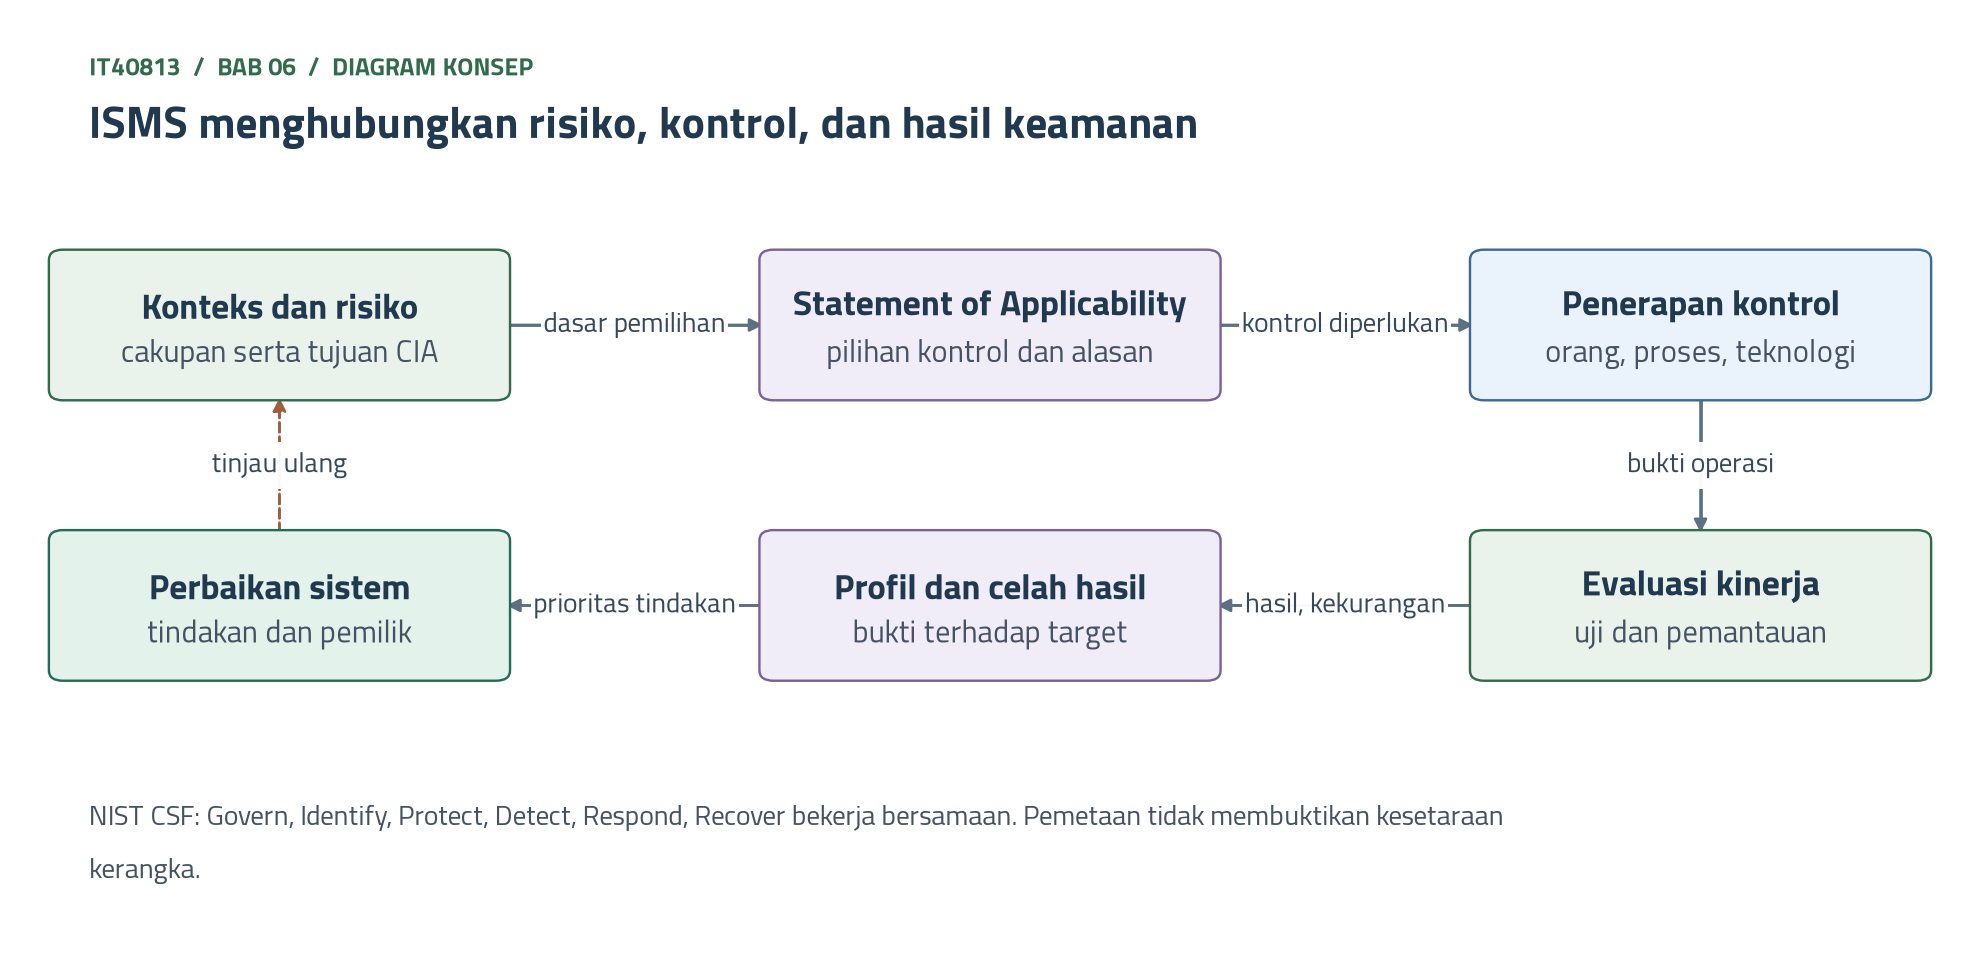
\includegraphics[width=\textwidth]{../figures/ch06-diagram-konsep.png}
  \caption{ISMS menghubungkan risiko, kontrol, dan hasil keamanan}
  \label{fig:ch06-ilustrasi-bab}
\end{figure}
}{}

\section{Kerahasiaan, Integritas, dan Ketersediaan}

\subsection*{Tiga tujuan pelindungan}

Keamanan informasi melindungi kerahasiaan, integritas, dan ketersediaan. Ketiganya sering disingkat
CIA, dari \textit{confidentiality}, \textit{integrity}, dan \textit{availability}. Kerahasiaan
membatasi siapa yang boleh membaca. Integritas menjaga ketepatan data serta perubahan yang sah.
Ketersediaan memastikan informasi dapat dipakai ketika diperlukan. Ketiga tujuan itu dapat saling
berbenturan, sehingga konfliknya diselesaikan sesuai konteks layanan.

Analogi lemari obat membantu menjelaskan pilihan. Lemari terkunci mengurangi akses yang tidak sah.
Pencatatan keluar masuk menjaga ketepatan stok. Kunci cadangan dan petugas pengganti menjaga
layanan ketika pemegang kunci utama tidak hadir.

Dua contoh memperlihatkan mengapa kontrol tidak cukup dinilai dari kerahasiaan:
\begin{enumerate}
  \item Misalkan satu akun bersama dipakai 12 petugas sebuah bangsal, dan dalam sebulan tercatat
  40 perubahan riwayat alergi. Sistem selalu tersedia dan tidak ada pihak luar yang membaca data.
  Namun, tidak satu pun dari 40 perubahan itu dapat ditelusuri kepada petugas tertentu.
  Kelemahannya ada pada integritas, dan kaitannya ada pada R-02 di register Bab 5.
  \item Misalkan semua akses darurat diblokir ketika pengelola identitas terganggu selama 2 jam.
  Data terlindung dari akses biasa, tetapi dokter tidak dapat membaca riwayat pengobatan. Bab 5
  menghitung gangguan 2 jam menyentuh sekitar 548 kunjungan. Akses darurat yang terbatas,
  beralasan, dan ditinjau menjadi pilihan yang perlu diuji.
\end{enumerate}

Tabel~\ref{tab:ch06-tiga-tujuan} merangkum tujuan pelindungan, pertanyaan layanan, dan bukti
contoh. Kode R-01, R-02, dan R-05 mengikuti register Bab 5.

\begin{table}[!htb]
  \centering\small
  \caption{Tujuan pelindungan dan bukti layanan}\label{tab:ch06-tiga-tujuan}
  \begin{tabularx}{\textwidth}{|>{\raggedright\arraybackslash}p{0.17\textwidth}|>{\raggedright\arraybackslash}X|>{\raggedright\arraybackslash}X|>{\raggedright\arraybackslash}p{0.09\textwidth}|}
    \hline
    \textbf{Tujuan} & \textbf{Pertanyaan} & \textbf{Bukti contoh} & \textbf{Risiko} \\ \hline
    Kerahasiaan & Apakah vendor hanya melihat data penugasannya? & Persetujuan dan pembatasan
    akses & R-01 \\ \hline
    Integritas & Siapa mengubah alergi dan kapan? & Jejak perubahan yang terlindungi & R-02 \\
    \hline
    Ketersediaan & Apakah data dapat dibaca saat gangguan? & Hasil uji pemulihan dan akses darurat
    & R-05 \\ \hline
  \end{tabularx}
\end{table}

\subsection*{Ketersediaan di rumah sakit: membaca satu penelitian}

Pertanyaan kemudian muncul: apakah gangguan ketersediaan di rumah sakit dapat diukur? Ghafur dan
rekan menelaah serangan \textit{ransomware} WannaCry 2017 pada National Health Service (NHS) Inggris
dengan data statistik episode rumah sakit \cite{c06-ghafur2019}. Penelitian itu memberi dua
pembacaan:
\begin{enumerate}
  \item Dampak terukur dalam layanan dan biaya. Pada 34 \textit{trust} rumah sakit yang terinfeksi,
  sekitar 13.500 janji rawat jalan dibatalkan pada pekan serangan. Pendaftaran gawat darurat turun
  sekitar 4 persen, dan pendaftaran elektif turun sekitar 9 persen, dihitung per hari per rumah
  sakit. Kerugian kegiatan diperkirakan £5,9 juta: £4 juta dari rawat inap, £0,6 juta dari gawat
  darurat, dan £1,3 juta dari rawat jalan.
  \item Satu ukuran tidak cukup. Penulis tidak menemukan kenaikan kematian, tetapi menyebut kematian
  sebagai ukuran kasar bagi bahaya terhadap pasien. Temuan itu tidak membuktikan serangan tanpa
  akibat klinis.
\end{enumerate}

Angka NHS tidak boleh disalin menjadi perkiraan kerugian Medikara, karena ukuran layanan dan sistem
pembiayaannya berbeda. Nilainya ada pada cara mengukur. Ketersediaan dinyatakan sebagai janji temu,
pendaftaran, dan biaya, bukan hanya jam server yang berhenti.

Dua hal juga sering tertukar: keamanan dan privasi. Pembagiannya begini. NIST menggambarkan
keduanya sebagai dua lingkaran yang beririsan \cite{nistcsf2}. Kebocoran lewat akun vendor berada
pada irisan itu. Pemakaian data yang sah secara teknis untuk tujuan lain dapat menjadi masalah
privasi tanpa insiden keamanan apa pun. Bab 7 merinci sisi pelindungan data pribadi.

\section{Sistem Manajemen ISO/IEC 27001}

\subsection*{Klausul 4 sampai 10}

Sistem manajemen keamanan informasi, atau ISMS, menghubungkan kebijakan, risiko, pelaksanaan,
evaluasi, dan perbaikan. ISO/IEC 27001 menetapkan persyaratan sistem manajemen itu. Klausul 4
sampai 10 mencakup konteks, kepemimpinan, perencanaan, dukungan, operasi, evaluasi kinerja, dan
perbaikan \cite{iso27001-2022}. Daftar alat dan kumpulan dokumen belum membentuk ISMS. Hubungan
antarbagian itulah yang diperiksa.

Analogi pengelolaan kebersihan dapur menunjukkan bedanya dengan daftar alat. Memiliki cairan
pembersih belum memastikan dapur bersih. Jadwal, pelaksana, pemeriksaan, penanganan kegagalan, dan
peninjauan pengelola membentuk sistem kerja.

Dua contoh membedakan kegiatan dan sistem:
\begin{enumerate}
  \item Misalkan tim membeli alat pemantauan untuk 5 rumah sakit. Tiap rumah sakit menghasilkan 300
  alarm per bulan, sehingga totalnya 1.500 alarm. Bila satu alarm ditelaah 10 menit, pekerjaannya
  250 jam per bulan, atau lebih dari satu orang penuh waktu dengan 160 jam kerja per bulan. Tanpa
  petugas, kriteria eskalasi, dan jadwal pemeriksaan, alarm hanya menjadi pesan yang menumpuk.
  Kekurangannya ada pada klausul dukungan dan operasi, bukan pada alat.
  \item Misalkan AC-01 dijalankan setiap bulan. Bulan pertama 24 dari 120 akun dicabut. Pemilik
  layanan membahas temuan itu dan menemukan sebabnya: tanggal berakhir penugasan tidak masuk
  daftar. Prosedur keluar vendor diubah, lalu jumlah pencabutan turun menjadi 9, 5, dan 2 akun pada
  tiga peninjauan berikutnya, atau turun sekitar 92 persen dari angka awal. Hubungan pelaksanaan,
  evaluasi, dan perbaikan menjadi terlihat.
\end{enumerate}

Gambar~\ref{fig:ch06-sistem} memperlihatkan urutan klausul tersebut. Gambar ini merupakan ringkasan
pembelajaran, bukan reproduksi isi standar. Singkatan SoA pada gambar berarti \textit{Statement of
Applicability}, yang dibahas pada seksi berikutnya. Tabel~\ref{tab:ch06-klausul} menerapkan tiap
klausul pada AC-01. Kode AC-01 mengikuti Bab 1, yaitu peninjauan akses berkala.

\begin{figure}[!htb]
  \centering
  \begin{tikzpicture}[
  font=\scriptsize,
  tahap/.style={draw, rounded corners, align=center, text width=2.35cm,
    minimum height=1.25cm, fill=blue!8},
  panah/.style={-{Stealth[length=2mm]}, thick}]
  \node[tahap, fill=praditagreen!15] (k4) at (0,0)
    {\textbf{Klausul 4}\\Konteks\\{\tiny\mdseries cakupan dan pihak terkait}};
  \node[tahap] (k5) at (3.05,0)
    {\textbf{Klausul 5}\\Kepemimpinan\\{\tiny\mdseries kebijakan dan peran}};
  \node[tahap] (k6) at (6.1,0)
    {\textbf{Klausul 6}\\Perencanaan\\{\tiny\mdseries risiko, SoA, sasaran}};
  \node[tahap] (k7) at (9.15,0)
    {\textbf{Klausul 7}\\Dukungan\\{\tiny\mdseries orang dan dokumen}};
  \node[tahap] (k8) at (9.15,-2.0)
    {\textbf{Klausul 8}\\Operasi\\{\tiny\mdseries kontrol dijalankan}};
  \node[tahap, fill=orange!12] (k9) at (6.1,-2.0)
    {\textbf{Klausul 9}\\Evaluasi kinerja\\{\tiny\mdseries uji, audit, tinjauan}};
  \node[tahap, fill=green!10] (k10) at (3.05,-2.0)
    {\textbf{Klausul 10}\\Perbaikan\\{\tiny\mdseries koreksi yang diverifikasi}};
  \draw[panah] (k4) -- (k5);
  \draw[panah] (k5) -- (k6);
  \draw[panah] (k6) -- (k7);
  \draw[panah] (k7) -- (k8);
  \draw[panah] (k8) -- (k9);
  \draw[panah] (k9) -- (k10);
  \draw[panah, dashed] (k10.west) -| node[pos=0.75, left, align=right]
    {tinjau\\ulang} (k4.south);
\end{tikzpicture}

  \caption{Klausul 4 sampai 10 sebagai satu sistem kerja}
  \label{fig:ch06-sistem}
\end{figure}

\begin{table}[!htb]
  \centering\small
  \caption{Klausul ISO/IEC 27001 pada kontrol AC-01 (misalkan)}\label{tab:ch06-klausul}
  \begin{tabularx}{\textwidth}{|>{\raggedright\arraybackslash}p{0.2\textwidth}|>{\raggedright\arraybackslash}X|>{\raggedright\arraybackslash}X|}
    \hline
    \textbf{Klausul} & \textbf{Pertanyaan} & \textbf{Bukti pada AC-01} \\ \hline
    4 Konteks & Sistem, lokasi, dan pihak mana yang masuk cakupan? & 5 rumah sakit, Medikara+, 120
    akun vendor; kewajiban K-01 \\ \hline
    5 Kepemimpinan & Siapa menetapkan kebijakan dan peran? & Kebijakan akses vendor; direksi
    menerima risiko sisa R-01 \\ \hline
    6 Perencanaan & Risiko dan kontrol apa yang dipilih? & R-01 dengan skor $3 \times 4 = 12$; baris
    SoA; sasaran nol akun tanpa pemilik \\ \hline
    7 Dukungan & Apakah orang dan dokumen cukup? & Peninjau yang ditunjuk; prosedur tertulis \\
    \hline
    8 Operasi & Apakah kontrol dijalankan? & Daftar akun, penandaan pemilik layanan, tiket
    pencabutan \\ \hline
    9 Evaluasi kinerja & Apakah kontrol bekerja? & 108 dari 120 akun tercakup; audit 6 dari 30 akun;
    tinjauan pimpinan \\ \hline
    10 Perbaikan & Apa yang berubah karena temuan? & Prosedur keluar vendor diubah; hasil diuji ulang
    \\ \hline
  \end{tabularx}
\end{table}

Keputusan membaca ISMS sebagai sistem punya dua konsekuensi. Pertama, temuan 12 akun yang luput
tidak ditutup hanya dengan mencabut 12 akun. Tim juga memeriksa mengapa daftar peninjau hanya memuat
108 akun. Kedua, kebijakan yang bagus tidak menaikkan penilaian bila catatan operasinya tidak ada.

Diagram konsep pada awal bab meringkas alur yang sama. Konteks dan risiko memberi dasar pemilihan
kontrol. SoA mencatat kontrol yang diperlukan. Penerapan kontrol menghasilkan bukti operasi. Evaluasi
kinerja menguji bukti itu, lalu hasil dan kekurangannya masuk ke profil dan celah hasil. Prioritas
tindakan menggerakkan perbaikan sistem, dan hasilnya ditinjau ulang.

Amandemen 1:2024 hanya mengubah dua subklausul. Rancangan adopsi Badan Standardisasi Nasional (BSN)
memuat teksnya. Subklausul 4.1 menambahkan kewajiban menentukan apakah perubahan iklim adalah isu
yang relevan. Subklausul 4.2 menambahkan catatan bahwa pihak berkepentingan dapat mempunyai
persyaratan terkait perubahan iklim \cite{c06-bsn-amd1}. Misalkan banjir musiman mengancam ruang
server satu rumah sakit. Tim mencatat hasil penentuan itu pada konteks ISMS, lalu menilai akibatnya
bersama R-05.

\subsection*{Sertifikat dan ruang lingkup}

Sertifikasi menilai sistem dalam ruang lingkup tertentu. Pertanyaan kemudian muncul: apa yang
dibuktikan sertifikat bagi Medikara? Bab 3 sudah menunjukkan sertifikat tidak menjawab kewajiban
hukum seperti dasar pemrosesan data. Dua contoh berikut menunjukkan batas lainnya:
\begin{enumerate}
  \item Misalkan Medikara memegang sertifikat untuk pusat data. Ke-36 fasilitas layanan, yaitu 5
  rumah sakit, 18 klinik, 1 laboratorium, dan 12 apotek, berada di luar ruang lingkup itu. Aplikasi
  vendor juga tidak otomatis tercakup.
  \item Misalkan vendor Medikara+ memiliki sertifikat yang masih berlaku 14 bulan, tetapi ruang
  lingkupnya hanya pengembangan aplikasi. Akun dukungan vendor yang masuk ke data pasien tidak
  termasuk. Masa berlaku yang panjang tidak menutup celah cakupan tersebut.
\end{enumerate}

Tanggal, penerbit, ruang lingkup, dan temuan karena itu tetap harus diperiksa sebelum sertifikat
dipakai sebagai bukti. Bab 9 memakai pemeriksaan yang sama untuk penyedia cloud.

Literatur ilmiah membantu membaca klaim manfaat sertifikasi. Tinjauan literatur Culot dan rekan
mengelompokkan penelitian ISO/IEC 27001 ke lima fokus: hubungan dengan standar lain, motivasi
penerapan, masalah saat penerapan, hasil yang mungkin, dan faktor konteks \cite{c06-culot2021}. Pada
pembacaan bab ini, susunan itu berguna sebagai daftar pertanyaan. Tim yang mendengar klaim ``sudah
bersertifikat'' dapat bertanya: mengapa sertifikat diambil, masalah apa yang muncul, dan hasil apa
yang benar-benar teramati.

\section{Annex A, SoA, dan Panduan Kontrol}

\subsection*{Annex A sebagai rujukan pemeriksa}

Annex A merupakan rujukan kontrol. Isinya 93 kontrol dalam empat tema: organisasi, manusia, fisik,
dan teknologi \cite{iso27001-2022,c06-dqs-annexa}. Berkas Informative References dari NIST
mencantumkan nomor yang sama: 5.1 sampai 5.37, 6.1 sampai 6.8, 7.1 sampai 7.14, dan 8.1 sampai 8.34
\cite{c06-nist-irefs}. \textit{Statement of Applicability} (SoA) menjelaskan kontrol yang diperlukan,
alasan pemilihan, status penerapan, dan alasan pengecualian kontrol Annex A yang tidak dipilih.
Annex A dipakai untuk memeriksa bahwa tidak ada kontrol perlu yang terlewat, bukan sebagai daftar
yang otomatis wajib seluruhnya.

Analogi daftar perlengkapan perjalanan menjelaskan pemilihan. Perjalanan pegunungan dan perjalanan
kota membutuhkan perlengkapan berbeda. Barang yang tidak dibawa harus dinilai terhadap tujuan dan
kondisi, bukan dihapus agar daftar terlihat lengkap.

Tabel~\ref{tab:ch06-tema} merangkum keempat tema. Uraian topik ditulis ringkas oleh bab ini dan
bukan terjemahan resmi. Nomor kontrol mengikuti berkas NIST tersebut.

\begin{table}[!htb]
  \centering\small
  \caption{Empat tema Annex A dan contoh topik pada Medikara}\label{tab:ch06-tema}
  \begin{tabularx}{\textwidth}{|>{\raggedright\arraybackslash}p{0.09\textwidth}|>{\raggedright\arraybackslash}p{0.17\textwidth}|>{\raggedright\arraybackslash}p{0.09\textwidth}|>{\raggedright\arraybackslash}X|}
    \hline
    \textbf{Nomor} & \textbf{Tema} & \textbf{Jumlah} & \textbf{Contoh topik pada Medikara} \\ \hline
    5 & Organisasi & 37 & 5.18 hak akses; 5.19 dan 5.20 hubungan serta perjanjian pemasok; 5.26
    tanggapan insiden \\ \hline
    6 & Manusia & 8 & Pelatihan petugas dan tanggung jawab setelah penugasan berakhir \\ \hline
    7 & Fisik & 14 & Ruang server dan perangkat di 36 fasilitas \\ \hline
    8 & Teknologi & 34 & 8.5 autentikasi; 8.13 cadangan; 8.15 pencatatan; 8.16 pemantauan \\ \hline
    Total & & 93 & \\ \hline
  \end{tabularx}
\end{table}

Dua hal pada keluarga standar ini sering tertukar: persyaratan dan panduan. Pembagiannya begini.
ISO/IEC 27001 berjudul \textit{Requirements} dan menjadi dasar penilaian sistem manajemen. ISO/IEC
27002 memberi panduan penerapan kontrol, sehingga tidak menjadi target sertifikasi sistem manajemen
tersendiri \cite{iso27001-2022,iso27002-2022}. ISO 27799:2025 memberi kontrol keamanan informasi
beserta panduan penerapan untuk organisasi kesehatan, dengan dasar ISO/IEC 27002 \cite{iso27799-2025}.
Tabel~\ref{tab:ch06-standar} membandingkan ketiganya.

\begin{table}[!htb]
  \centering\small
  \caption{Tiga standar dan pemakaiannya pada Medikara}\label{tab:ch06-standar}
  \begin{tabularx}{\textwidth}{|>{\raggedright\arraybackslash}p{0.2\textwidth}|>{\raggedright\arraybackslash}p{0.24\textwidth}|>{\raggedright\arraybackslash}X|}
    \hline
    \textbf{Standar} & \textbf{Sifat} & \textbf{Pemakaian pada Medikara} \\ \hline
    ISO/IEC 27001:2022 & Persyaratan sistem manajemen & Menilai ruang lingkup ISMS, SoA, evaluasi,
    dan perbaikan \\ \hline
    ISO/IEC 27002:2022 & Panduan penerapan kontrol & Menjelaskan cara merancang peninjauan hak akses
    pada AC-01 \\ \hline
    ISO 27799:2025 & Panduan kontrol untuk organisasi kesehatan & Membaca kontrol untuk rekam medis
    elektronik, perangkat digital fasilitas, dan telekonsultasi Medikara+ \\ \hline
  \end{tabularx}
\end{table}

\subsection*{Dari risiko ke SoA}

Pertanyaan berikutnya: dari mana kontrol dalam SoA berasal? Dari penanganan risiko. Tim memilih
penanganan, menetapkan kontrol yang diperlukan, lalu membandingkannya dengan Annex A.
Gambar~\ref{fig:ch06-rantai-soa} memperlihatkan rantai itu untuk R-01. Hasilnya berupa bukti operasi
yang dapat diuji.

\begin{figure}[!htb]
  \centering
  \begin{tikzpicture}[
  font=\scriptsize,
  tahap/.style={draw, rounded corners, align=center, text width=3.0cm,
    minimum height=1.1cm, fill=blue!8},
  panah/.style={-{Stealth[length=2mm]}, thick}]
  \node[tahap, fill=praditagreen!15] (risiko) at (0,0)
    {\textbf{Risiko R-01}\\{\tiny\mdseries skor $3 \times 4 = 12$, dinilai pada Bab 5}};
  \node[tahap] (tangani) at (4.1,0)
    {\textbf{Penanganan dipilih}\\{\tiny\mdseries kurangi paparan akun vendor}};
  \node[tahap] (perlu) at (8.2,0)
    {\textbf{Kontrol diperlukan}\\{\tiny\mdseries AC-01 dan pemantauan aktivitas}};
  \node[tahap] (banding) at (8.2,-1.9)
    {\textbf{Dibandingkan dengan Annex A}\\{\tiny\mdseries 93 kontrol sebagai rujukan}};
  \node[tahap, fill=orange!12] (soa) at (4.1,-1.9)
    {\textbf{SoA}\\{\tiny\mdseries kontrol, alasan, status, pengecualian}};
  \node[tahap, fill=green!10] (bukti) at (0,-1.9)
    {\textbf{Bukti operasi}\\{\tiny\mdseries daftar akun, keputusan, tiket pencabutan}};
  \draw[panah] (risiko) -- (tangani);
  \draw[panah] (tangani) -- (perlu);
  \draw[panah] (perlu) -- (banding);
  \draw[panah] (banding) -- (soa);
  \draw[panah] (soa) -- (bukti);
  \draw[panah, dashed] (bukti) -- node[right, align=left] {tinjau ulang} (risiko);
\end{tikzpicture}

  \caption{Rantai dari risiko ke SoA dan bukti operasi}
  \label{fig:ch06-rantai-soa}
\end{figure}

Dua contoh menguji alasan pemilihan:
\begin{enumerate}
  \item Misalkan akses vendor diperlukan untuk perbaikan. AC-01 dipilih karena R-01 dan K-01. Bukti
  mencakup daftar hak akses, peninjau yang sah, hasil keputusan, dan pencabutan. Status pada SoA
  ditulis ``diterapkan sebagian'', karena 12 dari 120 akun luput dan bukti peninjauan baru ada pada
  1 dari 5 rumah sakit.
  \item Misalkan Medikara tidak mengembangkan satu aplikasi sendiri, lalu mengusulkan pengecualian
  kontrol pengembangan. Sekitar 28.000 janji temu per bulan berjalan pada Medikara+ buatan vendor,
  dan R-07 menyebut perubahan yang tidak diuji. Pengadaan dan perubahan oleh vendor tetap menimbulkan
  kebutuhan kontrol, misalnya 8.30 tentang pengembangan alih daya dan 8.32 tentang manajemen
  perubahan. Usulan itu belum dapat diterima.
\end{enumerate}

Tabel~\ref{tab:ch06-soa} merangkum penalaran SoA tersebut sebagai ringkasan pembelajaran. Berkas
\berkas{sources/chapter06/catatan-soa.md} menyediakan lembar isiannya.

\begin{table}[!htb]
  \centering\small
  \caption{Contoh penalaran SoA (ringkasan pembelajaran)}\label{tab:ch06-soa}
  \begin{tabularx}{\textwidth}{|>{\raggedright\arraybackslash}p{0.25\textwidth}|>{\raggedright\arraybackslash}X|>{\raggedright\arraybackslash}X|}
    \hline
    \textbf{Kontrol} & \textbf{Alasan} & \textbf{Status dan bukti} \\ \hline
    Peninjauan hak akses, AC-01 (Annex A 5.18) & Mengurangi akses vendor berlebih pada R-01;
    mendukung K-01 & Diterapkan sebagian; bukti baru 1 dari 5 rumah sakit \\ \hline
    Pencatatan aktivitas (Annex A 8.15) & Menelusuri perubahan data pada R-01 dan R-02 & Catatan ada;
    perlindungan dan tinjauan belum terbukti \\ \hline
    Cadangan dan pemulihan (Annex A 8.13) & Menjaga data saat gangguan pada R-05; mendukung K-02 &
    Cadangan tersedia; hasil uji pemulihan diminta \\ \hline
    Pengembangan alih daya (Annex A 8.30) & Vendor mengubah Medikara+; R-07 & Usulan pengecualian
    ditolak; kontrol dinilai pada kontrak vendor \\ \hline
  \end{tabularx}
\end{table}

Keputusan mengecualikan kontrol punya dua konsekuensi. Pertama, alasannya harus dapat diuji
peninjau, sehingga kalimat ``tidak relevan'' saja tidak cukup. Kedua, pengecualian perlu ditinjau
ulang ketika cakupan berubah. Skenario Bab 4 menambah dua fasilitas, dari 36 menjadi 38, sehingga
baris yang menyangkut lokasi harus dibaca ulang.

Kode juga sering tertukar. AC-01 pada bab ini adalah kode lokal Medikara. Angka 5.18 adalah nomor
kontrol Annex A. Berkas NIST juga memuat label AC-01 milik NIST Special Publication (SP) 800-53 pada
subkategori PR.AA-05 \cite{c06-nist-irefs}, dan label itu bukan kontrol Medikara. Register sebaiknya
selalu menulis sumber kode, supaya pembaca tidak menganggap ketiganya satu kontrol yang sama.

\subsection*{Konteks kesehatan}

Cakupan ISO 27799:2025 meliputi perangkat lunak kesehatan seperti sistem rekam medis elektronik, dan
perangkat medis yang mengandung perangkat lunak. Standar itu berlaku pada organisasi kesehatan dari
segala jenis dan ukuran, termasuk layanan jarak jauh \cite{iso27799-2025}. Medikara dengan 36
fasilitas dan telekonsultasi berada dalam gambaran itu. Penilaian karena itu melibatkan pimpinan
klinis. Pembatasan akses tidak boleh merusak kebutuhan pelayanan darurat. NIST juga mencontohkan
akses darurat pada PR.AA-03: petugas yang berwenang tetap dapat mengakses akun yang penting bagi
keselamatan \cite{c06-nist-irefs}. Persetujuan pengecualian dan peninjauan setelah kejadian tetap
diperlukan.

Bab 5 sudah membatasi pengecualian darurat pada akun vendor paling lama 24 jam. Misalkan dalam
sebulan terjadi 6 pengecualian seperti itu pada 120 akun. Keenamnya ditinjau pemilik layanan pada
hari kerja berikutnya. Bila hanya 4 yang punya catatan alasan, kontrol bukan berjalan 67 persen,
melainkan ada 2 pengecualian yang tidak dapat dipertanggungjawabkan.

\begin{kasus}[title={Kasus Medikara Health: Menyusun SoA untuk Cakupan Terbatas}]
Misalkan tim menilai 93 kontrol untuk cakupan 5 rumah sakit dan Medikara+. Hasil awalnya 84 kontrol
diperlukan dan 9 kontrol diusulkan dikecualikan, atau sekitar 9,7 persen. Peninjau menguji kesembilan
usulan dengan register Bab 5. Tiga usulan ditolak karena R-07 menunjukkan vendor tetap mengubah
Medikara+. Hasil akhirnya 87 kontrol diperlukan dan 6 dikecualikan.

Keputusan ini punya dua konsekuensi. Pertama, pekerjaan bertambah 3 baris yang harus punya pemilik
dan bukti. Kedua, keenam pengecualian tersisa ditulis dengan alasan, pihak yang menyetujui, dan
tanggal tinjau ulang. Jumlah kontrol yang diperlukan bukan ukuran keamanan. Kualitas alasannya yang
dinilai.
\end{kasus}

\section{Enam Fungsi NIST CSF 2.0}

\subsection*{Struktur inti}

NIST CSF 2.0 menyusun hasil keamanan dalam hierarki fungsi, kategori, dan subkategori. Hitungan bab
ini pada lampiran naskahnya menghasilkan 6 fungsi, 22 kategori, dan 106 subkategori. Enam fungsinya
adalah Govern, Identify, Protect, Detect, Respond, dan Recover. Hasil itu bukan daftar periksa
tindakan. Urutannya juga tidak menyatakan urutan kerja atau tingkat kepentingan. Fungsi perlu
ditangani bersamaan. Kerangka ini menjelaskan hasil yang diinginkan tanpa menetapkan cara
mencapainya \cite{nistcsf2}.

Analogi pengamanan gedung menunjukkan hubungan antarfungsi. Pengelola menetapkan aturan, mendata
ruangan, memasang pengamanan, mendeteksi gangguan, menanganinya, lalu memulihkan penggunaan. Pintu
yang kuat tidak menggantikan petugas dan rencana penanganan.

Gambar~\ref{fig:ch06-enam-fungsi} menempatkan Govern di tengah, karena fungsi itu menjadi dasar cara
lima fungsi lain dijalankan. Gambar ini digambar ulang untuk bab ini.
Tabel~\ref{tab:ch06-fungsi} merangkum hasil tiap fungsi dan pertanyaan bagi Medikara.

\begin{figure}[!htb]
  \centering
  \begin{tikzpicture}[
  font=\scriptsize,
  fungsi/.style={draw, rounded corners, align=center, text width=2.2cm,
    minimum height=0.95cm, fill=blue!8},
  panah/.style={-{Stealth[length=2mm]}, thick}]
  \node[fungsi, fill=praditagreen!15, text width=2.7cm, minimum height=1.2cm] (gv) at (0,0)
    {\textbf{Govern}\\{\tiny\mdseries arah, peran, kebijakan, pengawasan, pemasok}};
  \node[fungsi] (id) at (0,2.3) {\textbf{Identify}\\{\tiny\mdseries aset, risiko, perbaikan}};
  \node[fungsi] (pr) at (4.2,0.8) {\textbf{Protect}\\{\tiny\mdseries akses, data, platform}};
  \node[fungsi] (de) at (2.55,-2.0) {\textbf{Detect}\\{\tiny\mdseries pemantauan, analisis}};
  \node[fungsi] (rs) at (-2.55,-2.0) {\textbf{Respond}\\{\tiny\mdseries insiden, komunikasi}};
  \node[fungsi] (rc) at (-4.2,0.8) {\textbf{Recover}\\{\tiny\mdseries pemulihan, komunikasi}};
  \draw[gray, thin] (id) -- (pr) -- (de) -- (rs) -- (rc) -- (id);
  \draw[panah] (gv) -- (id);
  \draw[panah] (gv) -- (pr);
  \draw[panah] (gv) -- (de);
  \draw[panah] (gv) -- (rs);
  \draw[panah] (gv) -- (rc);
\end{tikzpicture}

  \caption{Govern mengarahkan lima fungsi lain yang saling berhubungan}
  \label{fig:ch06-enam-fungsi}
\end{figure}

\begin{table}[!htb]
  \centering\small
  \caption{Hasil dan pertanyaan penilaian pada enam fungsi}\label{tab:ch06-fungsi}
  \begin{tabularx}{\textwidth}{|>{\raggedright\arraybackslash}p{0.14\textwidth}|>{\raggedright\arraybackslash}X|>{\raggedright\arraybackslash}X|>{\raggedright\arraybackslash}p{0.23\textwidth}|}
    \hline
    \textbf{Fungsi} & \textbf{Hasil (ringkasan)} & \textbf{Pertanyaan Medikara} & \textbf{Bukti contoh}
    \\ \hline
    Govern & Strategi, harapan, dan kebijakan risiko ditetapkan serta dipantau & Siapa menerima
    risiko akses vendor? & Keputusan dan wewenang \\ \hline
    Identify & Risiko keamanan saat ini dipahami & Sistem dan data apa yang terlibat? & Inventaris
    serta alur data \\ \hline
    Protect & Pengaman dipakai untuk mengelola risiko & Bagaimana akses dibatasi? & Daftar hak dan
    bukti AC-01 \\ \hline
    Detect & Kemungkinan serangan ditemukan dan dianalisis & Bagaimana akses menyimpang diketahui? &
    Catatan alarm dan tinjauan \\ \hline
    Respond & Tindakan atas insiden yang terdeteksi diambil & Siapa membekukan akses? & Prosedur dan
    hasil latihan \\ \hline
    Recover & Aset dan operasi yang terdampak dipulihkan & Bagaimana data dipulihkan? & Hasil uji
    pemulihan \\ \hline
  \end{tabularx}
\end{table}

Dua contoh menunjukkan fungsi yang saling melengkapi:
\begin{enumerate}
  \item Misalkan seluruh 108 akun pada daftar peninjau memakai Multi-Factor Authentication (MFA).
  Cakupannya tampak 100 persen. Terhadap populasi 120 akun, cakupannya hanya 90 persen, karena 12
  akun tidak tercatat. Protect yang kuat tidak menolong bila Identify belum lengkap.
  \item Misalkan alarm akses diterima dalam 5 menit. Tanpa petugas yang berwenang membekukan akun,
  kecepatan deteksi belum menghasilkan penanganan. Data latihan Bab 1 memberi pembandingnya: akun
  dukungan memanggil data selama 8 malam dan baru diketahui pada hari ke-11.
\end{enumerate}

Inventaris pada ID.AM-02 juga mencakup layanan \textit{Application Programming Interface} (API) dan
layanan cloud \cite{c06-nist-irefs}. Bab ini cukup memastikan keduanya masuk cakupan profil. Cara
mengamankan API dibahas pada mata kuliah IT40613, dan keamanan cloud pada IT40713.

\subsection*{Mengapa Govern ditambahkan}

Versi 1.1 memiliki lima fungsi: Identify, Protect, Detect, Respond, dan Recover
\cite{c06-nist-csf11}. Versi 2.0 menambahkan Govern dan menonjolkan tata kelola serta rantai pasok
\cite{nistcsf2}. Masalah organisasi apa yang ingin diselesaikan? NIST menulis bahwa kegiatan tata
kelola penting untuk memasukkan keamanan ke strategi risiko enterprise, dan bahwa pimpinan
mengomunikasikan harapan tentang \textit{risk appetite}, akuntabilitas, dan sumber daya. Tanpa fungsi
ini, penilaian keamanan mudah berhenti sebagai urusan tim teknis. Kalimat terakhir merupakan
penafsiran bab ini.

Tabel~\ref{tab:ch06-govern} menautkan kategori Govern dengan hasil kerja bab sebelumnya. Enam
kategori pada Govern adalah konteks organisasi (GV.OC), strategi pengelolaan risiko (GV.RM), peran
dan wewenang (GV.RR), kebijakan (GV.PO), pengawasan (GV.OV), dan pengelolaan risiko rantai pasok
(GV.SC).

\begin{table}[!htb]
  \centering\small
  \caption{Subkategori Govern dan hasil kerja bab sebelumnya}\label{tab:ch06-govern}
  \begin{tabularx}{\textwidth}{|>{\raggedright\arraybackslash}p{0.14\textwidth}|>{\raggedright\arraybackslash}X|>{\raggedright\arraybackslash}X|}
    \hline
    \textbf{Subkategori} & \textbf{Hasil (ringkasan)} & \textbf{Hasil kerja Medikara} \\ \hline
    GV.OC-03 & Persyaratan hukum, regulasi, dan kontrak dipahami serta dikelola & Register K-01
    sampai K-16 pada Bab 3 \\ \hline
    GV.RM-02 & Pernyataan \textit{risk appetite} dan \textit{risk tolerance} ditetapkan & Batas nol
    akun vendor aktif tanpa pemilik pada Bab 5 \\ \hline
    GV.RR-02 & Peran, tanggung jawab, dan wewenang ditetapkan serta ditegakkan & Hak keputusan akses
    vendor pada Bab 2 \\ \hline
    GV.SC-07 & Risiko pemasok dipahami dan dipantau sepanjang hubungan & Vendor Medikara+, R-01, dan
    insiden 2025 \\ \hline
  \end{tabularx}
\end{table}

\subsection*{ISO/IEC 27001 dan NIST CSF}

Dua kerangka ini juga sering tertukar. Pembagiannya begini. ISO/IEC 27001 menetapkan persyaratan yang
dapat dinilai dalam ruang lingkup tertentu. NIST CSF menyediakan bahasa hasil yang dapat dipakai
secara sukarela atau lewat kebijakan pemerintah, dan naskah 2.0 tidak memuat skema sertifikasi
\cite{nistcsf2}. Tabel~\ref{tab:ch06-iso-csf} menunjukkan bahwa keduanya melengkapi, bukan
menggantikan.

\begin{table}[!htb]
  \centering\small
  \caption{Perbedaan ISO/IEC 27001 dan NIST CSF 2.0}\label{tab:ch06-iso-csf}
  \begin{tabularx}{\textwidth}{|>{\raggedright\arraybackslash}p{0.17\textwidth}|>{\raggedright\arraybackslash}X|>{\raggedright\arraybackslash}X|}
    \hline
    \textbf{Pembeda} & \textbf{ISO/IEC 27001:2022} & \textbf{NIST CSF 2.0} \\ \hline
    Sifat & Persyaratan sistem manajemen & Taksonomi hasil, tanpa menetapkan cara \\ \hline
    Unsur & Klausul 4 sampai 10, 93 kontrol Annex A, SoA & 6 fungsi, 22 kategori, 106 subkategori,
    profil, \textit{tier} \\ \hline
    Pemeriksaan & Dapat disertifikasi dalam ruang lingkup & Tidak ada skema sertifikasi pada naskah
    2.0 \\ \hline
    Akses naskah & Berbayar & Terbuka \\ \hline
    Luaran Medikara & Ruang lingkup ISMS, SoA, hasil evaluasi & Profil saat ini, celah, profil target
    Bab 8 \\ \hline
  \end{tabularx}
\end{table}

\section{Profil Saat Ini dan Tier}

\subsection*{Profil organisasi}

Profil organisasi menggambarkan keadaan keamanan saat ini atau target dalam bahasa hasil pada CSF.
Profil saat ini (\textit{Current Profile}) menyebut hasil yang sedang dicapai dan seberapa jauh hasil
itu tercapai. Profil target (\textit{Target Profile}) menyebut hasil yang dipilih dan diprioritaskan
\cite{nistcsf2}. Satu organisasi dapat memiliki beberapa profil, masing-masing dengan cakupan berbeda.
Setiap kesimpulan memerlukan bukti dan catatan batasnya.

Analogi potret cabang toko menunjukkan pentingnya cakupan. Foto satu rak yang rapi tidak menunjukkan
seluruh toko. Potret harus menjelaskan rak, tanggal, dan bagian yang tidak terlihat.

NIST menyarankan lima langkah: menetapkan cakupan, mengumpulkan informasi, membuat profil,
menganalisis celah serta menyusun rencana tindakan, lalu menjalankan rencana dan memperbarui profil
\cite{nistcsf2,c06-nist-sp1301}. Gambar~\ref{fig:ch06-langkah-profil} menerapkannya pada Medikara.
Templat NIST memuat kolom praktik, status, peringkat, prioritas, dan sasaran, dan kolom itu boleh
disesuaikan \cite{c06-nist-sp1301}. Bab ini mengerjakan langkah 1 sampai 4 untuk profil saat ini.
Profil target dirancang pada Bab 8.

\begin{figure}[!htb]
  \centering
  \begin{tikzpicture}[
  font=\scriptsize,
  tahap/.style={draw, rounded corners, align=center, text width=1.9cm,
    minimum height=1.0cm, fill=blue!8},
  hasil/.style={draw, align=center, text width=1.9cm, minimum height=1.05cm,
    fill=white, font=\tiny},
  panah/.style={-{Stealth[length=2mm]}, thick}]
  \node[tahap] (s1) at (0,0) {1. Tetapkan cakupan};
  \node[tahap] (s2) at (2.45,0) {2. Kumpulkan informasi};
  \node[tahap, fill=orange!12] (s3) at (4.9,0) {3. Buat profil};
  \node[tahap, fill=orange!12] (s4) at (7.35,0) {4. Analisis celah dan rencana};
  \node[tahap, fill=green!10] (s5) at (9.8,0) {5. Jalankan dan perbarui};
  \node[hasil] (h1) at (0,-1.55) {5 rumah sakit, Medikara+, 120 akun, 12 bulan};
  \node[hasil] (h2) at (2.45,-1.55) {Register Bab 3, register Bab 5, sumber bukti};
  \node[hasil] (h3) at (4.9,-1.55) {14 subkategori dengan status lokal};
  \node[hasil] (h4) at (7.35,-1.55) {6 celah, 3 prioritas untuk Bab 8};
  \node[hasil] (h5) at (9.8,-1.55) {Profil target Bab 8, tonggak C3};
  \draw[panah] (s1) -- (s2);
  \draw[panah] (s2) -- (s3);
  \draw[panah] (s3) -- (s4);
  \draw[panah] (s4) -- (s5);
  \foreach \nomor in {1,2,3,4,5} {
    \draw[gray, thin] (s\nomor) -- (h\nomor);
  }
  \draw[panah, dashed] (s5.north) -- ++(0,0.4) -| node[pos=0.25, above] {ulangi} (s1.north);
\end{tikzpicture}

  \caption{Lima langkah membuat dan memakai profil, dengan keluaran Medikara (misalkan)}
  \label{fig:ch06-langkah-profil}
\end{figure}

Dua contoh menguji kualitas klaim:
\begin{enumerate}
  \item Audit Bab 4 memeriksa 30 akun, dan 24 di antaranya sesuai, atau 80 persen. Tim menyimpulkan
  ada 6 pengecualian dalam sampel. Tim tidak menyatakan seluruh organisasi 80 persen aman. Angka 24
  dari 120 akun berasal dari peninjauan penuh, bukan dari proyeksi sampel. Daftarnya pun hanya memuat
  108 akun dan buktinya hanya ada pada 1 dari 5 rumah sakit.
  \item Misalkan cadangan berhasil dibuat setiap malam selama 30 hari pada 5 rumah sakit, sehingga
  ada 150 pekerjaan cadangan yang berhasil. Tim belum menyatakan pemulihan tercapai sebelum data
  dipulihkan dan pemilik layanan menguji kelengkapannya. PR.DS-11 meminta cadangan juga diuji, dan
  RC.RP-03 meminta integritas cadangan diverifikasi sebelum dipakai \cite{nistcsf2}.
\end{enumerate}

Tabel~\ref{tab:ch06-profil} merangkum status lokal yang dipakai tim. Daftar ini merupakan alat kerja
bab ini, bukan skala resmi NIST. NIST memberi contoh skala seperti tinggi, sedang, dan rendah, atau
1 sampai 5 \cite{c06-nist-sp1301}. Status lokal dipilih karena memisahkan ``belum terbukti'' dari
``gagal''.

\begin{table}[!htb]
  \centering\small
  \caption{Status lokal yang dipakai tim}\label{tab:ch06-profil}
  \begin{tabularx}{\textwidth}{|>{\raggedright\arraybackslash}p{0.2\textwidth}|>{\raggedright\arraybackslash}X|>{\raggedright\arraybackslash}X|}
    \hline
    \textbf{Status lokal} & \textbf{Arti} & \textbf{Tindakan} \\ \hline
    Terbukti & Bukti sesuai cakupan dan periode & Simpan sumber dan peninjau \\ \hline
    Sebagian & Sebagian hasil atau lokasi belum tercakup & Jelaskan celah spesifik \\ \hline
    Belum ada bukti & Klaim belum dapat diuji & Minta bukti; jangan beri status lulus \\ \hline
    Tidak relevan & Ada alasan terhadap cakupan & Catat persetujuan dan tinjau ulang \\ \hline
  \end{tabularx}
\end{table}

\subsection*{Contoh profil saat ini}

Misalkan tim Medikara memilih cakupan akses vendor dan SIMRS pada 5 rumah sakit serta Medikara+,
untuk periode 12 bulan. Tim memilih 14 dari 106 subkategori, atau sekitar 13,2 persen. Pemilihan
mengikuti konteks risiko, bukan keinginan memperindah hasil. Tabel~\ref{tab:ch06-profil-tata-kelola}
dan Tabel~\ref{tab:ch06-profil-teknis} menyajikan hasilnya. Teks hasil diringkas dari NIST
\cite{nistcsf2}.

\begin{table}[!htb]
  \centering\small
  \caption{Profil saat ini: Govern dan Identify (misalkan)}\label{tab:ch06-profil-tata-kelola}
  \begin{tabularx}{\textwidth}{|>{\raggedright\arraybackslash}p{0.14\textwidth}|>{\raggedright\arraybackslash}p{0.13\textwidth}|>{\raggedright\arraybackslash}X|>{\raggedright\arraybackslash}p{0.13\textwidth}|}
    \hline
    \textbf{Subkategori} & \textbf{Status} & \textbf{Bukti dan batasnya} & \textbf{Tautan} \\ \hline
    GV.OC-03 & Sebagian & Register 16 baris ada; 7 baris belum diverifikasi & K-01 sampai K-16 \\
    \hline
    GV.RM-02 & Sebagian & Batas nol akun tanpa pemilik sudah dirumuskan; pemantauannya belum teruji &
    R-01 \\ \hline
    GV.RR-02 & Sebagian & Hak keputusan tertulis; 12 akun belum punya pemilik & R-01 \\ \hline
    GV.SC-07 & Sebagian & Vendor utama dikenal; tinjauan berkala belum ada; laporan insiden telat &
    R-01, R-08, K-05 \\ \hline
    ID.AM-02 & Sebagian & Daftar lokal 5 rumah sakit berbeda dan belum direkonsiliasi & R-02 \\ \hline
  \end{tabularx}
\end{table}

\begin{table}[!htb]
  \centering\small
  \caption{Profil saat ini: Protect sampai Recover (misalkan)}\label{tab:ch06-profil-teknis}
  \begin{tabularx}{\textwidth}{|>{\raggedright\arraybackslash}p{0.14\textwidth}|>{\raggedright\arraybackslash}p{0.13\textwidth}|>{\raggedright\arraybackslash}X|>{\raggedright\arraybackslash}p{0.13\textwidth}|}
    \hline
    \textbf{Subkategori} & \textbf{Status} & \textbf{Bukti dan batasnya} & \textbf{Tautan} \\ \hline
    PR.AA-01 & Sebagian & Akun per orang belum berlaku; akun bersama ditemukan & R-02, K-01 \\ \hline
    PR.AA-03 & Sebagian & MFA tercatat pada 108 akun; 12 akun tidak diketahui & R-01, K-01 \\ \hline
    PR.AA-05 & Sebagian & AC-01 berjalan; bukti pada 1 dari 5 rumah sakit & R-01, R-02, K-01 \\ \hline
    PR.AA-06 & Tidak relevan & Vendor bekerja jarak jauh pada cakupan ini; tinjau bila vendor hadir
    di lokasi & Tidak ada \\ \hline
    PR.PS-04 & Terbukti & Catatan aktivitas tersedia pada 5 SIMRS selama 12 bulan & R-01 \\ \hline
    PR.DS-11 & Sebagian & Cadangan malam berjalan; uji pemulihan belum ada & R-05, K-02 \\ \hline
    DE.CM-03 & Sebagian & Catatan tersedia; bukti tinjauan dan tindak lanjut belum ada & R-01, K-01 \\
    \hline
    RS.MA-01 & Belum ada bukti & Prosedur tertulis; belum dilatih bersama vendor & R-01, R-12, K-04,
    K-05 \\ \hline
    RC.RP-03 & Belum ada bukti & Hasil verifikasi cadangan belum tersedia & R-05, K-02 \\ \hline
  \end{tabularx}
\end{table}

Rekap status itu adalah 1 terbukti, 10 sebagian, 2 belum ada bukti, dan 1 tidak relevan. Rekap ini
punya dua konsekuensi. Pertama, angka itu tidak boleh dirata-rata menjadi satu nilai. Satu baris
``terbukti'' dari 14 baris tidak berarti keamanan Medikara sekitar 7 persen. Kedua, status ``tidak
relevan'' hanya berlaku pada cakupan ini. NIST menyebut cakupan profil menentukan apakah suatu hasil
berlaku \cite{c06-nist-sp1301}, sehingga PR.AA-06 kembali dinilai bila cakupan berubah.

\subsection*{Tier}

\textit{Tier} menggambarkan ketelitian tata kelola dan pengelolaan risiko keamanan organisasi. Ada
empat \textit{tier}: Partial, Risk Informed, Repeatable, dan Adaptive. \textit{Tier} melengkapi
metode pengelolaan risiko, bukan menggantikannya. Naskah NIST menyebut tabelnya sebagai ilustrasi
\cite{nistcsf2}. Pemilihan \textit{tier} umumnya dilakukan pimpinan organisasi. Memilih pada tingkat
keseluruhan, fungsi, atau kategori memberi gambaran yang lebih baik daripada pada tingkat subkategori
\cite{c06-nist-sp1302}.

Analoginya seperti cara keluarga mengatur keuangan. Ada yang mencatat seadanya, ada yang punya
anggaran tetapi hanya di kepala satu orang, ada yang menulis aturan bersama, dan ada yang terus
menyesuaikan anggaran dengan keadaan. Tingkat itu menjelaskan cara mengelola uang, bukan jumlah saldo
hari ini.

Tabel~\ref{tab:ch06-tier} meringkas keempatnya, lalu membacanya dari sisi risiko pemasok.

\begin{table}[!htb]
  \centering\small
  \caption{Empat \textit{tier} dan pembacaan risiko pemasok}\label{tab:ch06-tier}
  \begin{tabularx}{\textwidth}{|>{\raggedright\arraybackslash}p{0.2\textwidth}|>{\raggedright\arraybackslash}X|>{\raggedright\arraybackslash}X|}
    \hline
    \textbf{Tier} & \textbf{Tata kelola risiko (ringkasan)} & \textbf{Risiko pemasok (ringkasan)} \\
    \hline
    Tier 1, Partial & Strategi risiko diterapkan seadanya & Umumnya tidak menyadari risiko pemasok \\
    \hline
    Tier 2, Risk Informed & Praktik disetujui manajemen, tetapi mungkin belum menjadi kebijakan
    organisasi & Sadar risiko pemasok, tetapi belum bertindak konsisten atau formal \\ \hline
    Tier 3, Repeatable & Praktik disetujui resmi sebagai kebijakan dan diperbarui berkala & Strategi
    risiko mempertimbangkan pemasok; ada perjanjian tertulis dan pemantauan \\ \hline
    Tier 4, Adaptive & Risiko dipantau pimpinan bersama risiko keuangan dan risiko lain & Informasi
    hampir waktu nyata dipakai untuk bertindak atas risiko pemasok \\ \hline
  \end{tabularx}
\end{table}

Dua contoh memperlihatkan pemakaiannya:
\begin{enumerate}
  \item Misalkan pimpinan membaca kolom pemasok untuk fungsi Protect. Insiden 2025 membuat risiko
  vendor dikenal, tetapi AC-01 baru terbukti pada 1 dari 5 rumah sakit. Deskripsi itu paling dekat
  dengan Tier 2. Pembacaan ini merupakan penilaian pimpinan, bukan hasil hitungan dari 14 baris
  profil.
  \item Misalkan konsultan menawarkan rumus: status terbukti diberi nilai 4, sebagian nilai 2, dan
  belum ada bukti nilai 1. Tiga belas baris yang dinilai menghasilkan rata-rata 2,0, lalu ditulis
  ``Tier 2''. Rumus itu tidak punya dasar pada NIST. Angkanya tampak cocok dengan contoh pertama
  hanya karena kebetulan.
\end{enumerate}

Tiga hal pada penilaian ini sering tertukar: status lokal, \textit{tier}, dan tingkat kapabilitas
Control Objectives for Information and Related Technologies (COBIT). Pembagiannya begini. Ketiganya
menjawab pertanyaan yang berbeda, seperti pada Tabel~\ref{tab:ch06-tiga-ukuran}, dan tidak saling
dikonversi. Bab 8 memakai batas yang sama ketika menetapkan profil target dan target kapabilitas.

\begin{table}[!htb]
  \centering\small
  \caption{Tiga ukuran yang tidak saling dikonversi}\label{tab:ch06-tiga-ukuran}
  \begin{tabularx}{\textwidth}{|>{\raggedright\arraybackslash}p{0.22\textwidth}|>{\raggedright\arraybackslash}X|>{\raggedright\arraybackslash}X|}
    \hline
    \textbf{Ukuran} & \textbf{Yang dinilai} & \textbf{Contoh Medikara} \\ \hline
    Status lokal & Bukti satu hasil dalam cakupan profil & PR.AA-05 sebagian, karena bukti baru 1
    dari 5 rumah sakit \\ \hline
    \textit{Tier} & Ketelitian pengelolaan risiko pada organisasi, fungsi, atau kategori & Tier 2
    untuk Protect pada pembacaan pimpinan \\ \hline
    Tingkat kapabilitas COBIT & Kapabilitas proses pada objektif COBIT & Tingkat indikatif 1 untuk
    DSS05 lewat AC-01 pada satu rumah sakit, seperti Bab 4 \\ \hline
  \end{tabularx}
\end{table}

\begin{pendalaman}
Sampel 30 dari 120 akun memberi perkiraan, bukan kepastian. Bila sampel diambil acak, proporsi 6
dari 30 sama dengan 0,2. Galat baku dengan koreksi populasi terbatas adalah
$\sqrt{0{,}2 \times 0{,}8 / 30} \times \sqrt{90 / 119}$, atau sekitar 0,0635. Rentang kepercayaan 95
persen dengan pendekatan normal sekitar 0,2 ditambah atau dikurangi 0,124. Hasilnya 7,6 sampai 32,4
persen, atau sekitar 9 sampai 39 akun dari 120. Peninjauan penuh yang menemukan 24 akun berada di
dalam rentang itu. Hitungan ini tidak berlaku bila sampel dipilih karena mudah diperoleh, dan tidak
mencakup 12 akun yang tidak masuk daftar.
\end{pendalaman}

\section{Dari Bukti ke Celah Kontrol}

\subsection*{Pemetaan menunjukkan kontribusi}

Pemetaan menghubungkan hasil yang belum tercapai, kontrol, risiko, dan kewajiban. Hubungannya dapat
banyak ke banyak. NIST menyebut \textit{Informative References} sebagai pemetaan antara inti CSF dan
standar atau regulasi lain, dan sebagian rujukan lebih sempit dari subkategorinya \cite{nistcsf2}.
Pemetaan tidak membuktikan kesetaraan antarkerangka. Bukti yang cukup untuk satu tujuan audit belum
tentu cukup untuk tujuan lain.

Analogi peta angkutan memperlihatkan batasnya. Dua jalur melewati stasiun yang sama, tetapi memiliki
tujuan dan jam operasi berbeda. Kesamaan satu titik bukan kesamaan seluruh perjalanan.

Pertanyaan kemudian muncul: seberapa jauh pemetaan dapat dipercaya? Panduan NIST SP 1347 memberi tiga
peringatan. Rujukan pada katalog Online Informative References (OLIR) disusun NIST dan pihak lain.
NIST tidak menguji kebenaran pemetaan dari pihak lain, dan pencantuman tidak berarti dukungan NIST.
Hubungan turunan antardokumen pun tidak bersifat otoritatif \cite{c06-nist-sp1347}. Panduan yang sama
mencontohkan organisasi pemakai CSF 2.0 yang ingin mengadopsi ISO/IEC 27001. Organisasi itu menyaring
hasil pemetaan, lalu bertanya hasil mana yang sudah tercapai, mana yang belum, mana yang bertentangan,
dan sumber daya apa yang diperlukan. Tim karena itu memperlakukan pemetaan sebagai titik awal.

Dua contoh menghasilkan keputusan yang berbeda:
\begin{enumerate}
  \item Misalkan AC-01 baru punya bukti pada 1 dari 5 rumah sakit. Dengan peninjauan bulanan selama
  12 bulan, seharusnya ada 60 catatan, dan yang tersedia 12, atau 20 persen. Celahnya adalah cakupan
  peninjauan. Membeli alat baru belum menjamin pemilik layanan menyetujui seluruh hak akses.
  \item Misalkan seluruh lokasi mempunyai catatan akses dan aturan organisasi meminta tinjauan
  mingguan. Selama 52 minggu pada 5 rumah sakit, seharusnya ada 260 catatan tinjauan, dan yang
  tersedia nol. Celahnya adalah proses deteksi dan tindak lanjut, bukan sekadar penyimpanan catatan.
\end{enumerate}

Tabel~\ref{tab:ch06-pemetaan} menautkan sebagian subkategori dengan nomor Annex A dari berkas NIST,
kontrol Medikara, risiko, dan kewajiban \cite{c06-nist-irefs,uu27-2022-pdp,permenkes24-2022}. Kolom
kewajiban mengikuti register Bab 3. K-01 berasal dari Pasal 39 Undang-Undang (UU) 27/2022 tentang
Pelindungan Data Pribadi (PDP), dan K-02 dari Permenkes 24/2022 Pasal 20. Tautan ke kontrol, risiko,
dan kewajiban merupakan pengandaian bab ini.

\begin{table}[!htb]
  \centering\small
  \caption{Pemetaan subkategori ke Annex A, kontrol, risiko, dan kewajiban}\label{tab:ch06-pemetaan}
  \begin{tabularx}{\textwidth}{|>{\raggedright\arraybackslash}p{0.14\textwidth}|>{\raggedright\arraybackslash}p{0.21\textwidth}|>{\raggedright\arraybackslash}X|>{\raggedright\arraybackslash}p{0.2\textwidth}|}
    \hline
    \textbf{Subkategori} & \textbf{Annex A} & \textbf{Kontrol Medikara} & \textbf{Risiko, kewajiban}
    \\ \hline
    PR.AA-05 & 5.15, 5.18, 8.2, 8.3, 8.18 & AC-01 peninjauan akses & R-01, R-02, K-01 \\ \hline
    PR.AA-01 & 5.15, 5.16, 5.18, 8.2, 8.5 & Akun per orang & R-02, K-01 \\ \hline
    PR.AA-03 & 5.15, 5.16, 5.17, 5.18, 8.5 & MFA akun vendor & R-01, K-01 \\ \hline
    ID.AM-02 & 5.9 & Inventaris sistem lintas rumah sakit & R-02 \\ \hline
    PR.PS-04 & 8.15, 8.17 & Pencatatan aktivitas & R-01, K-01 \\ \hline
    DE.CM-03 & 7.4, 8.16 & Tinjauan catatan aktivitas & R-01, K-01 \\ \hline
    PR.DS-11 & 8.13 & Cadangan di lokasi terpisah & R-05, K-02 \\ \hline
    RC.RP-03 & 8.13 & Uji pemulihan & R-05, K-02 \\ \hline
    RS.MA-01 & 5.26, 5.27, 5.28 & Prosedur insiden bersama vendor & R-01, R-12, K-04, K-05 \\ \hline
    GV.SC-07 & 5.19, 5.20, 5.22, 5.31 & Tinjauan vendor & R-01, R-08, K-05 \\ \hline
  \end{tabularx}
\end{table}

Dua hal perlu dibaca dari tabel itu. Berkas NIST memuat dua daftar untuk PR.AA-05. Daftar pertama
berisi 11 kontrol, daftar kedua berisi 6 kontrol, dan keduanya hanya bertemu pada 5 kontrol. Tabel
di atas memakai irisan itu, lalu daftar lengkapnya tersedia di
\berkas{sources/chapter06/pemetaan-csf-annex-a.csv}. Selain itu, tujuan pemetaan tidak selalu kontrol
Annex A. DE.CM-03 juga dipetakan ke klausul 9.1, dan GV.RR-02 ke klausul 7.2 \cite{c06-nist-irefs}.
Sebagian celah karena itu berujung pada perbaikan sistem manajemen.

\subsection*{Menyusun daftar celah}

Pertanyaan berikutnya: celah dibandingkan dengan apa? Analisis celah pada CSF membandingkan profil
saat ini dan profil target \cite{nistcsf2}. Profil target baru dirancang pada Bab 8. Bab ini karena
itu memakai pembanding sementara: batas \textit{risk appetite} Bab 5, kewajiban pada register Bab 3,
dan kontrol yang diperlukan pada SoA. Rencana tindakan yang baik memuat tindakan, prioritas, pemilik,
tenggat, dan sumber daya \cite{c06-nist-sp1301}.

Tabel~\ref{tab:ch06-celah} merangkum enam celah. Kolom pemilik memisahkan pemilik risiko dan pemilik
tindakan. Pemilik R-02 tetap pemilik SIMRS sesuai Bab 5, sedangkan kepala teknologi informasi (TI)
memimpin tindakan inventaris. Gambar~\ref{fig:ch06-keterlacakan} menelusuri tiga celah prioritas dari
subkategori sampai kewajiban.

\begin{table}[!htb]
  \centering\small
  \caption{Hubungan celah dan risiko (misalkan)}\label{tab:ch06-celah}
  \begin{tabularx}{\textwidth}{|>{\raggedright\arraybackslash}p{0.08\textwidth}|>{\raggedright\arraybackslash}X|>{\raggedright\arraybackslash}p{0.13\textwidth}|>{\raggedright\arraybackslash}p{0.2\textwidth}|>{\raggedright\arraybackslash}X|}
    \hline
    \textbf{ID} & \textbf{Hasil belum tercapai} & \textbf{Risiko} & \textbf{Pemilik risiko; pemilik
    tindakan} & \textbf{Bukti penerimaan} \\ \hline
    G-01 & Peninjauan belum lintas lokasi; 12 dari 120 akun luput & R-01, K-01 & Pemilik Medikara+;
    kepala operasi TI & 120 dari 120 akun cocok; peninjauan 5 rumah sakit \\ \hline
    G-02 & Catatan aktivitas tidak ditinjau & R-01, K-01 & Pemilik Medikara+; fungsi keamanan & Alarm
    uji ditangani dalam latihan \\ \hline
    G-03 & Pemulihan belum diuji & R-05, K-02 & Pemilik layanan; kepala operasi TI & Data contoh
    pulih; hasil disahkan pemilik layanan \\ \hline
    G-04 & Hak lokal berbeda; akun bersama masih ada & R-02, K-01 & Pemilik SIMRS; pemilik layanan &
    Peran baku pada 5 rumah sakit; nol akun bersama pada sampel \\ \hline
    G-05 & Vendor terlambat melapor; prosedur belum dilatih & R-01, R-12, K-04, K-05 & Pemilik
    Medikara+; pengelola vendor & Latihan bersama: laporan dalam 12 jam \\ \hline
    G-06 & Inventaris lokal belum direkonsiliasi & R-02 & Pemilik SIMRS; kepala TI & Satu inventaris
    disetujui untuk 5 rumah sakit \\ \hline
  \end{tabularx}
\end{table}

\begin{figure}[!htb]
  \centering
  \begin{tikzpicture}[
  font=\scriptsize,
  judul/.style={draw, align=center, text width=1.9cm, minimum height=0.6cm,
    fill=praditagreen!15},
  sel/.style={draw, rounded corners, align=center, text width=1.9cm,
    minimum height=1.05cm, fill=blue!8},
  panah/.style={-{Stealth[length=2mm]}, thick}]
  \node[judul] at (0,0) {\textbf{Subkategori}};
  \node[judul] at (2.45,0) {\textbf{Status lokal}};
  \node[judul] at (4.9,0) {\textbf{Celah}};
  \node[judul] at (7.35,0) {\textbf{Kontrol}};
  \node[judul] at (9.8,0) {\textbf{Risiko, kewajiban}};
  \node[sel] (a1) at (0,-1.0) {PR.AA-05};
  \node[sel, fill=gray!35] (a2) at (2.45,-1.0) {Sebagian};
  \node[sel, fill=orange!12] (a3) at (4.9,-1.0)
    {\textbf{G-01}\\{\tiny\mdseries peninjauan belum lintas lokasi}};
  \node[sel] (a4) at (7.35,-1.0) {AC-01\\{\tiny\mdseries Annex A 5.15, 5.18}};
  \node[sel, fill=green!10] (a5) at (9.8,-1.0) {R-01, K-01};
  \node[sel] (b1) at (0,-2.3) {RC.RP-03};
  \node[sel, fill=red!22] (b2) at (2.45,-2.3) {Belum ada bukti};
  \node[sel, fill=orange!12] (b3) at (4.9,-2.3)
    {\textbf{G-03}\\{\tiny\mdseries pemulihan belum diuji}};
  \node[sel] (b4) at (7.35,-2.3) {Uji pemulihan\\{\tiny\mdseries Annex A 8.13}};
  \node[sel, fill=green!10] (b5) at (9.8,-2.3) {R-05, K-02};
  \node[sel] (c1) at (0,-3.6) {RS.MA-01, GV.SC-07};
  \node[sel, fill=red!22] (c2) at (2.45,-3.6) {Belum ada bukti};
  \node[sel, fill=orange!12] (c3) at (4.9,-3.6)
    {\textbf{G-05}\\{\tiny\mdseries vendor terlambat\\melapor}};
  \node[sel] (c4) at (7.35,-3.6) {Insiden vendor\\{\tiny\mdseries Annex A 5.20, 5.26}};
  \node[sel, fill=green!10] (c5) at (9.8,-3.6) {R-01, R-12, K-04, K-05};
  \foreach \baris in {a,b,c} {
    \draw[panah] (\baris1) -- (\baris2);
    \draw[panah] (\baris2) -- (\baris3);
    \draw[panah] (\baris3) -- (\baris4);
    \draw[panah] (\baris4) -- (\baris5);
  }
\end{tikzpicture}

  \caption{Keterlacakan tiga celah prioritas (misalkan)}
  \label{fig:ch06-keterlacakan}
\end{figure}

\begin{kasus}[title={Kasus Medikara Health: Tiga Prioritas untuk Bab 8}]
Bab 5 menetapkan tiga prioritas risiko: R-11 karena keselamatan pasien, R-01 karena insiden 2025 dan
K-01, serta R-05 karena harapan kerugiannya paling besar. R-11 berakar pada pertukaran data, sehingga
tetap berada pada jalur pimpinan klinis. Misalkan tim memilih G-01 untuk R-01 dan G-03 untuk R-05. Tim
menambah G-05, karena K-05 berstatus tidak memenuhi: pada varian uji kontrak Bab 3, vendor baru
melapor setelah 30 jam, sedangkan kontrak meminta 12 jam.

Keputusan ini punya dua konsekuensi yang dapat dihitung. Pertama, bila mencocokkan satu akun memerlukan
6 menit, G-01 memakan 12 jam per bulan untuk 120 akun, atau 144 jam per tahun. Bab 5 menganggarkan
Rp60 juta untuk perluasan AC-01. Kedua, Bab 3 mengandaikan 144 uji pemulihan per tahun, yaitu satu uji
per fasilitas per triwulan pada 36 fasilitas. Bila satu uji memerlukan 3 jam, G-03 memakan 432 jam per
tahun. Keduanya berjumlah 576 jam, atau sekitar 3,6 bulan kerja dari 52 staf TI. Beban itu terjangkau,
tetapi harus dijadwalkan dan tidak bisa bergantung pada tim platform 6 orang. Rincian kelangsungan
layanan menunggu Bab 10, karena DSS04 ditunda ke sana.
\end{kasus}

\begin{pendalaman}
Bagian ini opsional dan hanya untuk sistem milik tim atau sistem dengan izin tertulis. Jangan
menjalankan pemindaian atau uji apa pun pada sistem pihak lain tanpa izin itu. Pilih satu kontrol
teknis, misalnya cakupan MFA. Ambil populasi dari sumber yang tidak bergantung pada sistem yang
diperiksa, misalnya daftar penugasan. Hitung akun yang memenuhi dibagi populasi: 108 dari 120 akun
berarti 90 persen, bukan 100 persen. Catat pengecualian dan tanggal pengambilan bukti.

Pilihan lain adalah konfigurasi pencatatan terhadap CIS Benchmarks dari Center for Internet Security
(CIS), yaitu rekomendasi konfigurasi preskriptif untuk lebih dari 25 keluarga produk
\cite{c06-cis-benchmarks}. Misalkan tim memeriksa 20 rekomendasi pencatatan pada 5 SIMRS, sehingga ada
100 baris, dan 72 baris sesuai. Laporkan juga 28 baris yang tersisa beserta alasannya. Pemetaan
antarkerangka dapat memakai katalog OLIR atau CSF 2.0 Reference Tool \cite{c06-nist-sp1347}. Kesimpulan
tetap memerlukan pengujian.
\end{pendalaman}

\section{Aktivitas: Profil Keamanan Saat Ini dan Daftar Celah}

\textbf{Tujuan.} Tim menyusun profil saat ini NIST CSF 2.0 dan daftar celah kontrol yang dapat
dipertanggungjawabkan. Tim memakai organisasi nyata dengan izin dan data yang dianonimkan, atau kasus
Medikara Health.

\textbf{Pembagian peran.} Analis teknologi memimpin penilaian dan memilih subkategori. Pemilik konteks
memastikan buktinya benar ada dan mengesahkan sumbernya. Analis regulasi menandai kontrol yang juga
diwajibkan regulasi, dengan register Bab 3. Analis risiko menjaga hubungan dengan register Bab 5.

\textbf{Langkah kerja.}
\begin{enumerate}
  \item Tetapkan sistem, lokasi, periode, dan pembatasan akses bukti. Untuk Medikara, fokusnya kontrol
  akses SIMRS lintas rumah sakit, pengelolaan akun vendor, pencatatan \textit{log}, dan cadangan data.
  \item Salin \berkas{sources/chapter06/profil-csf-saat-ini.csv}. Mulai dari 14 subkategori yang
  tersedia, lalu tambah atau kurangi sesuai cakupan. Keenam fungsi harus terwakili, dan alasan
  pemilihan dicatat.
  \item Kumpulkan bukti dengan \berkas{sources/chapter06/panduan-bukti.md}. Jangan menyalin data
  pasien.
  \item Beri status terbukti, sebagian, belum ada bukti, atau tidak relevan. Bandingkan dengan
  \berkas{sources/chapter06/contoh-profil-medikara.csv} sebagai pembanding skenario, bukan bukti
  organisasi.
  \item Isi \berkas{sources/chapter06/celah-kontrol.csv}. Cari nomor Annex A dengan
  \berkas{sources/chapter06/pemetaan-csf-annex-a.csv}, lalu cocokkan ke naskah berlisensi bila
  tersedia.
  \item Hubungkan setiap celah dengan risiko, kontrol, kewajiban, pemilik risiko, pemilik tindakan,
  dan bukti penerimaan. Tulis ``perlu analisis'' bila hubungan itu belum dapat dipastikan.
  \item Tinjau alasan pemilihan dan pengecualian dengan \berkas{sources/chapter06/catatan-soa.md}.
  \item Pilih tiga prioritas beserta alasannya, lalu serahkan kepada tim perancang profil target
  Bab 8.
\end{enumerate}

\textbf{Luaran.} Profil saat ini, daftar celah terhadap kontrol Annex A, catatan SoA, dan tiga
prioritas.

\textbf{Kaitan dengan capstone.} Luaran masuk tonggak C2 Kondisi Saat Ini, yang ditinjau menjelang
Ujian Tengah Semester. Daftar celah dipakai lagi pada Bab 8 untuk profil target, Bab 9 untuk risiko
pihak ketiga, Bab 10 untuk kelangsungan layanan, dan Bab 12 untuk pengujian kontrol.

\textbf{Kriteria penilaian.} Cakupan dan bukti 35 persen; penalaran status 25 persen; keterlacakan
risiko 25 persen; batas kesimpulan 15 persen. Nilai tinggi diberikan pada kejujuran celah dan kualitas
bukti, bukan banyaknya status terbukti.

\textbf{Berkas pendukung.} Daftar lengkap ada di \berkas{sources/chapter06/README.md}. Data organisasi
nyata wajib berizin dan dianonimkan. Data pribadi pasien atau karyawan, kata sandi, dan token tidak
boleh disalin. Pendalaman teknis pada kotak di atas bersifat opsional dan terpisah dari penilaian
utama.

\section{Ringkasan}

Keamanan informasi menjaga kerahasiaan, integritas, dan ketersediaan sesuai tujuan layanan. Dalam
kesehatan, kontrol harus dinilai bersama dampaknya pada pasien dan akses darurat. Akun bersama dapat
merusak jejak perubahan alergi tanpa kebocoran apa pun, dan pemblokiran total dapat menyentuh ratusan
kunjungan. Penelitian tentang WannaCry menunjukkan ketersediaan dapat diukur sebagai janji temu,
pendaftaran, dan biaya.

ISMS menghubungkan risiko, kontrol, evaluasi, dan perbaikan melalui klausul 4 sampai 10. Kebijakan
serta pembelian alat belum membuktikan sistem berjalan. Temuan 12 dari 120 akun yang luput baru selesai
ketika sebab pada daftar peninjau diperbaiki dan hasilnya diuji. Ruang lingkup sertifikat harus
diperiksa, karena sertifikat pusat data tidak menjawab 36 fasilitas layanan.

Annex A memberi 93 kontrol rujukan dalam empat tema, dan SoA mencatat alasan pemilihan serta
pengecualian. ISO/IEC 27002 memberi panduan penerapan, sedangkan ISO 27799 menempatkannya dalam konteks
kesehatan. Pengecualian yang baik dapat diuji peninjau dan ditinjau ulang ketika cakupan berubah.

NIST CSF 2.0 memberi bahasa hasil dalam 6 fungsi, dengan Govern sebagai dasar lima fungsi lainnya.
Profil saat ini menyampaikan hasil yang tercapai dan bukti yang belum ada. \textit{Tier} menggambarkan
ketelitian pengelolaan risiko, bukan rata-rata status kontrol. Status lokal, \textit{tier}, dan tingkat
kapabilitas COBIT tidak saling dikonversi.

Pemetaan menunjukkan kontribusi, bukan kesetaraan, sehingga tim memperlakukannya sebagai titik awal.
Daftar celah menautkan subkategori, kontrol, risiko, kewajiban, pemilik, dan bukti penerimaan. Tiga
prioritas Medikara menjadi masukan profil target Bab 8. Pesan utama bab ini sederhana: kesimpulan
keamanan harus sepadan dengan cakupan buktinya.

\section{Latihan}

\subsection*{Latihan 1: Persyaratan dan Panduan}

Jelaskan mengapa organisasi dapat disertifikasi terhadap ISO/IEC 27001, tetapi tidak terhadap ISO/IEC
27002. Latihan ini membuktikan bahwa kedua standar menilai objek yang berbeda.

\begin{enumerate}
  \item Baca deskripsi resmi kedua standar dan catat kata pada judulnya.
  \item Pilih AC-01 sebagai contoh kontrol.
  \item Pisahkan hal yang diperiksa pada sistem manajemen dari panduan cara menerapkan kontrol.
  \item Uji pemisahan itu dengan temuan 6 dari 30 akun dan 12 dari 120 akun.
\end{enumerate}

Tabel~\ref{tab:ch06-lat1-contoh} merangkum contoh analisis Latihan 1 dari skenario pembelajaran, dan
Tabel~\ref{tab:ch06-lat1-hasil} menyediakan lembar isiannya.

\begin{table}[!htb]
  \centering\small
  \caption{Contoh analisis Latihan 1 (skenario pembelajaran)}\label{tab:ch06-lat1-contoh}
  \begin{tabularx}{\textwidth}{|>{\raggedright\arraybackslash}p{0.2\textwidth}|>{\raggedright\arraybackslash}X|>{\raggedright\arraybackslash}X|}
    \hline
    \textbf{Rujukan} & \textbf{Objek} & \textbf{Bukti contoh} \\ \hline
    ISO/IEC 27001 & Sistem manajemen dalam cakupan & Evaluasi risiko R-01, baris SoA, dan perbaikan
    daftar 108 menjadi 120 akun \\ \hline
    ISO/IEC 27002 & Panduan kontrol & Cara meninjau hak akses dan mencabut akun \\ \hline
  \end{tabularx}
\end{table}

\begin{table}[!htb]
  \centering\small
  \caption{Lembar hasil Latihan 1}\label{tab:ch06-lat1-hasil}
  \begin{tabularx}{\textwidth}{|>{\raggedright\arraybackslash}p{0.2\textwidth}|>{\raggedright\arraybackslash}X|>{\raggedright\arraybackslash}X|}
    \hline
    \textbf{Rujukan} & \textbf{Objek} & \textbf{Bukti contoh} \\ \hline
    \dots & \dots & \dots \\ \hline
    \dots & \dots & \dots \\ \hline
  \end{tabularx}
\end{table}

\textbf{Pertanyaan analisis.} Audit menemukan 6 dari 30 akun bermasalah, dan bukti peninjauan hanya
ada pada 1 dari 5 rumah sakit: bagian mana menyentuh sistem manajemen, dan bagian mana menyentuh cara
menerapkan kontrol? Bila sertifikat hanya mencakup pusat data, bukti apa yang masih diminta untuk 36
fasilitas layanan?

\subsection*{Latihan 2: Peran Govern}

Fungsi Govern ditambahkan pada NIST CSF 2.0. Masalah organisasi apa yang ingin diselesaikan dengan
penambahan itu? Latihan ini membuktikan bahwa sebagian celah keamanan berakar pada keputusan, bukan
pada alat.

\begin{enumerate}
  \item Telusuri satu keputusan keamanan vendor dari permintaan sampai pencabutan akses.
  \item Identifikasi pemilik risiko dan batas keputusannya pada register Bab 5.
  \item Tentukan subkategori Govern yang belum tercapai.
  \item Hubungkan keputusan dengan pelaksanaan kontrol pada fungsi lain.
\end{enumerate}

Tabel~\ref{tab:ch06-lat2-contoh} merangkum contoh analisis Latihan 2 dari skenario pembelajaran, dan
Tabel~\ref{tab:ch06-lat2-hasil} menyediakan lembar isiannya.

\begin{table}[!htb]
  \centering\small
  \caption{Contoh analisis Latihan 2 (skenario pembelajaran)}\label{tab:ch06-lat2-contoh}
  \begin{tabularx}{\textwidth}{|>{\raggedright\arraybackslash}X|>{\raggedright\arraybackslash}X|>{\raggedright\arraybackslash}X|}
    \hline
    \textbf{Keadaan (misalkan)} & \textbf{Celah organisasi} & \textbf{Perbaikan} \\ \hline
    MFA pada 108 akun; 12 akun tidak punya pemilik & Akuntabilitas tidak jelas (GV.RR-02) & Tetapkan
    pemilik dan tinjau AC-01 \\ \hline
    Alarm tiba dalam 5 menit; tidak ada yang berwenang membekukan akun & Wewenang belum ditetapkan
    (GV.RR-02) & Beri wewenang kepada petugas jaga; uji eskalasi \\ \hline
    Vendor melapor setelah 30 jam; kontrak 12 jam & Risiko pemasok tidak dipantau (GV.SC-07) & Tinjau
    kontrak dan latih insiden bersama \\ \hline
  \end{tabularx}
\end{table}

\begin{table}[!htb]
  \centering\small
  \caption{Lembar hasil Latihan 2}\label{tab:ch06-lat2-hasil}
  \begin{tabularx}{\textwidth}{|>{\raggedright\arraybackslash}X|>{\raggedright\arraybackslash}X|>{\raggedright\arraybackslash}X|}
    \hline
    \textbf{Keadaan (misalkan)} & \textbf{Celah organisasi} & \textbf{Perbaikan} \\ \hline
    \dots & \dots & \dots \\ \hline
    \dots & \dots & \dots \\ \hline
  \end{tabularx}
\end{table}

\textbf{Pertanyaan analisis.} Pada baris pertama, berapa persen cakupan MFA terhadap populasi 120
akun, dan mengapa menambah alat belum memperbaikinya? Pada baris ketiga, berapa jam kontrak terlewati?
Bukti apa menunjukkan direksi benar menindaklanjuti risiko itu?

\subsection*{Latihan 3: Pengecualian Kontrol}

Sebuah rumah sakit memutuskan tidak menerapkan satu kontrol Annex A. Apa yang harus ditulis di SoA agar
keputusan itu dapat dipertanggungjawabkan? Latihan ini membuktikan bahwa pengecualian adalah keputusan
yang punya alasan, pemilik, dan batas waktu.

\begin{enumerate}
  \item Tentukan cakupan dan risiko terkait.
  \item Uji kewajiban pada register Bab 3 serta alternatif kontrol.
  \item Catat alasan, pihak yang menyetujui, dan tanggal tinjau ulang.
  \item Tulis bukti yang akan membatalkan alasan tersebut.
\end{enumerate}

Tabel~\ref{tab:ch06-lat3-contoh} merangkum contoh analisis Latihan 3 dari skenario pembelajaran, dan
Tabel~\ref{tab:ch06-lat3-hasil} menyediakan lembar isiannya.

\begin{table}[!htb]
  \centering\small
  \caption{Contoh analisis Latihan 3 (skenario pembelajaran)}\label{tab:ch06-lat3-contoh}
  \begin{tabularx}{\textwidth}{|>{\raggedright\arraybackslash}X|>{\raggedright\arraybackslash}X|>{\raggedright\arraybackslash}X|}
    \hline
    \textbf{Usulan (misalkan)} & \textbf{Analisis} & \textbf{Keputusan dan isi SoA} \\ \hline
    Tidak ada pengembangan internal & Vendor tetap mengubah aplikasi; R-07 & Jangan mengecualikan tanpa
    menilai pengadaan dan perubahan \\ \hline
    Satu rumah sakit tanpa akses vendor selama 12 bulan & Daftar menunjukkan 0 akun; penugasan baru dapat
    muncul & Pengecualian lokal; alasan, penyetuju, tinjau tiap triwulan \\ \hline
  \end{tabularx}
\end{table}

\begin{table}[!htb]
  \centering\small
  \caption{Lembar hasil Latihan 3}\label{tab:ch06-lat3-hasil}
  \begin{tabularx}{\textwidth}{|>{\raggedright\arraybackslash}X|>{\raggedright\arraybackslash}X|>{\raggedright\arraybackslash}X|}
    \hline
    \textbf{Usulan (misalkan)} & \textbf{Analisis} & \textbf{Keputusan dan isi SoA} \\ \hline
    \dots & \dots & \dots \\ \hline
    \dots & \dots & \dots \\ \hline
  \end{tabularx}
\end{table}

\textbf{Pertanyaan analisis.} Pada baris kedua, angka berapa pada daftar akun akan membatalkan alasan
pengecualian? Bila Medikara bertambah dua fasilitas sehingga menjadi 38, baris SoA mana yang harus
ditinjau kembali, dan siapa yang menyetujuinya?

  \chapter{Pelindungan Data Pribadi dalam Praktik}

\section*{Tujuan Pembelajaran}
\begin{itemize}
  \item Menjelaskan kewajiban pengendali dan prosesor data pribadi menurut UU 27/2022 dan PP 33/2026.
  \item Menyusun catatan kegiatan pemrosesan data pribadi untuk satu proses layanan.
  \item Menganalisis insiden kebocoran data dan menilai apakah penanganannya memenuhi kewajiban notifikasi.
\end{itemize}

\section{Pendahuluan}

% TODO
% Cakupan: data pasien bocor lewat vendor, lalu muncul pertanyaan siapa yang bertanggung jawab dan apa yang wajib dilakukan dalam hitungan jam.
% Kasus Medikara: insiden kebocoran skala kecil lewat vendor pada 2025.

\section{Konsep Dasar UU 27/2022}

% TODO
% Cakupan: data pribadi umum dan data pribadi yang bersifat spesifik, termasuk data kesehatan; prinsip pemrosesan; dasar pemrosesan; ruang lingkup dan masa transisi yang berakhir 17 Oktober 2024.

\section{Hak Subjek Data dan Kewajiban Pengendali}

% TODO
% Cakupan: hak akses, pembetulan, penghapusan, dan keberatan atas keputusan otomatis; kewajiban pengendali dan prosesor; pengendali bersama; pejabat atau petugas pelindungan data pribadi.

\section{PP 33/2026 dan Status Penegakan}

% TODO
% Cakupan: ditetapkan 16 Juli 2026 dan berlaku 16 Januari 2027; rincian teknis seperti mekanisme persetujuan, data anak, penilaian dampak, transfer data, dan ganti rugi; sanksi administratif; status lembaga pengawas pelindungan data pribadi.
% Catatan: per 30 Oktober 2026 naskah resmi belum tampil di JDIH BPK; cocokkan nomor pasal dengan naskah resmi saat menulis isi.

\section{Penilaian Dampak dan Notifikasi Kegagalan}

% TODO
% Cakupan: kapan penilaian dampak pelindungan data pribadi wajib (data spesifik, skala besar, keputusan otomatis); isi minimum penilaian; notifikasi tertulis paling lambat 3 x 24 jam kepada subjek data dan lembaga; isi notifikasi.
% Kasus Medikara: garis waktu insiden vendor 2025 dibandingkan dengan kewajiban notifikasi.

\section{Catatan Kegiatan Pemrosesan dan Transfer Data}

% TODO
% Cakupan: struktur catatan kegiatan pemrosesan (RoPA, Records of Processing Activities); pemetaan alur data; transfer ke luar wilayah hukum Indonesia; kaitan dengan kerahasiaan dan masa simpan rekam medis menurut Permenkes 24/2022.
% Kasus Medikara: alur data pendaftaran pasien dan telekonsultasi di Medikara+.

\section{Sistem Manajemen Privasi ISO/IEC 27701:2025}

% TODO
% Cakupan: PIMS (Privacy Information Management System) yang kini dapat berdiri sendiri; kaitan dengan ISO/IEC 27001; kapan sertifikasi privasi berguna bagi organisasi.
% Pendalaman teknis: pseudonimisasi, tokenisasi, klasifikasi data otomatis, dan sumber daya Consent pada HL7 FHIR (dibahas rinci di IT40613).

\section{Aktivitas: Catatan Pemrosesan Data dan Analisis Insiden Vendor}

% TODO
% Tujuan aktivitas: memahami alur data pribadi yang sebenarnya dan menilai celah kepatuhan PDP berdasarkan satu proses dan satu insiden.
% Peran dalam tim: analis regulasi memimpin; pemilik konteks memetakan alur data nyata; analis teknologi menelusuri sistem yang terlibat; analis risiko memperbarui risk register.
% Langkah: pilih satu proses layanan; isi catatan pemrosesan (jenis data, tujuan, dasar, penerima, lokasi, masa simpan, kontrol); susun garis waktu insiden vendor 2025; nilai celah terhadap UU PDP dan PP 33/2026; rangkum seluruh luaran Bab 4 sampai 7 menjadi C2.
% Luaran dan tonggak capstone: catatan kegiatan pemrosesan data pribadi dan analisis celah PDP; masuk C2 yang ditinjau menjelang UTS.
% Berkas sources yang direncanakan: sources/chapter07/templat-ropa.xlsx, sources/chapter07/kronologi-insiden-vendor-2025.md, sources/chapter07/daftar-periksa-celah-pdp.xlsx

\section{Ringkasan}

% TODO

\section{Latihan}

\begin{enumerate}
  \item Medikara memakai vendor untuk aplikasi Medikara+. Dalam hubungan ini, siapa pengendali dan siapa prosesor? Apa akibatnya terhadap tanggung jawab saat terjadi kebocoran?
  \item Tentukan dasar pemrosesan yang paling tepat untuk data rekam medis dalam layanan pengobatan. Jelaskan mengapa persetujuan belum tentu menjadi dasar yang terbaik.
  \item Susun garis waktu notifikasi yang memenuhi UU PDP untuk insiden yang ditemukan pada Jumat malam.
\end{enumerate}

  % !TeX root = it-governance-risk-compliance.tex
% !TeX encoding = UTF-8
\chapter{Merancang Sistem Tata Kelola Target}

\section*{Tujuan Pembelajaran}
\begin{itemize}
  \item Merancang struktur tata kelola target, termasuk forum keputusan, peran kunci, dan
  matriks RACI.
  \item Menetapkan target kapabilitas COBIT dan profil target NIST CSF yang selaras dengan
  \textit{risk appetite}.
  \item Mengaitkan praktik ITIL 4 dengan objektif manajemen COBIT untuk menjalankan layanan TI
  sehari-hari.
\end{itemize}

\section{Pendahuluan}

Semua pimpinan Medikara menyetujui strategi Satu Pasien, Satu Rekam Medis. Perselisihan baru
muncul ketika keputusan nyata datang. Misalkan mitra asuransi meminta integrasi untuk 6.000
klaim per bulan. Tim platform teknologi informasi (TI) ingin segera membuka data, pemilik
layanan khawatir terhadap gangguan, dan fungsi hukum meminta pembatasan tujuan. Usulan itu
berpindah antarforum selama 4 bulan. Selama itu 24.000 klaim tetap diproses manual, dan belum
ada yang dapat menyebut siapa pemutusnya.

Medikara membutuhkan tata kelola yang menjawab dua pertanyaan: siapa menyetujui pembukaan data
kepada mitra, dan siapa memegang akuntabilitas atas rekam medis terpadu. Bab 4 sampai Bab 7
sudah memberi bahannya, yaitu enam objektif awal, 12 skenario risiko, 14 baris profil keamanan,
dan 13 celah. Bab ini mengubah bahan itu menjadi model tata kelola target untuk tonggak C3
capstone. Model tersebut harus menutup celah C2, sepadan dengan kemampuan organisasi, dan
terhubung dengan rancangan tiga mata kuliah lain.

Bab ini memakai panduan desain Control Objectives for Information and Related Technologies
(COBIT) 2019 untuk menetapkan target, National Institute of Standards and Technology
Cybersecurity Framework (NIST CSF) 2.0 untuk profil target keamanan, dan Information Technology
Infrastructure Library (ITIL) 4 untuk praktik layanan. ISO/IEC 38500:2024 dan Three Lines Model
dari The Institute of Internal Auditors (IIA) menjadi pegangan pembagian peran. ISO adalah
International Organization for Standardization, dan IEC adalah International Electrotechnical
Commission. Naskah COBIT, ITIL, dan ISO berbayar, sehingga rinciannya ditulis ringkas dan perlu
dicocokkan ke naskah berlisensi sebelum dipakai untuk penilaian formal. Publikasi NIST terbuka.
Pilihan target dan angka biaya merupakan skenario pembelajaran
\cite{cobit2019-design,nistcsf2,itil4,iso38500-2024,iia-tlm2026}.

\IfFileExists{../figures/ch08-diagram-konsep.png}{%

Gambar \ref{fig:ch08-ilustrasi-bab} merangkum hubungan komponen dan konsep utama bab ini.
\begin{figure}[!htb]
  \centering
  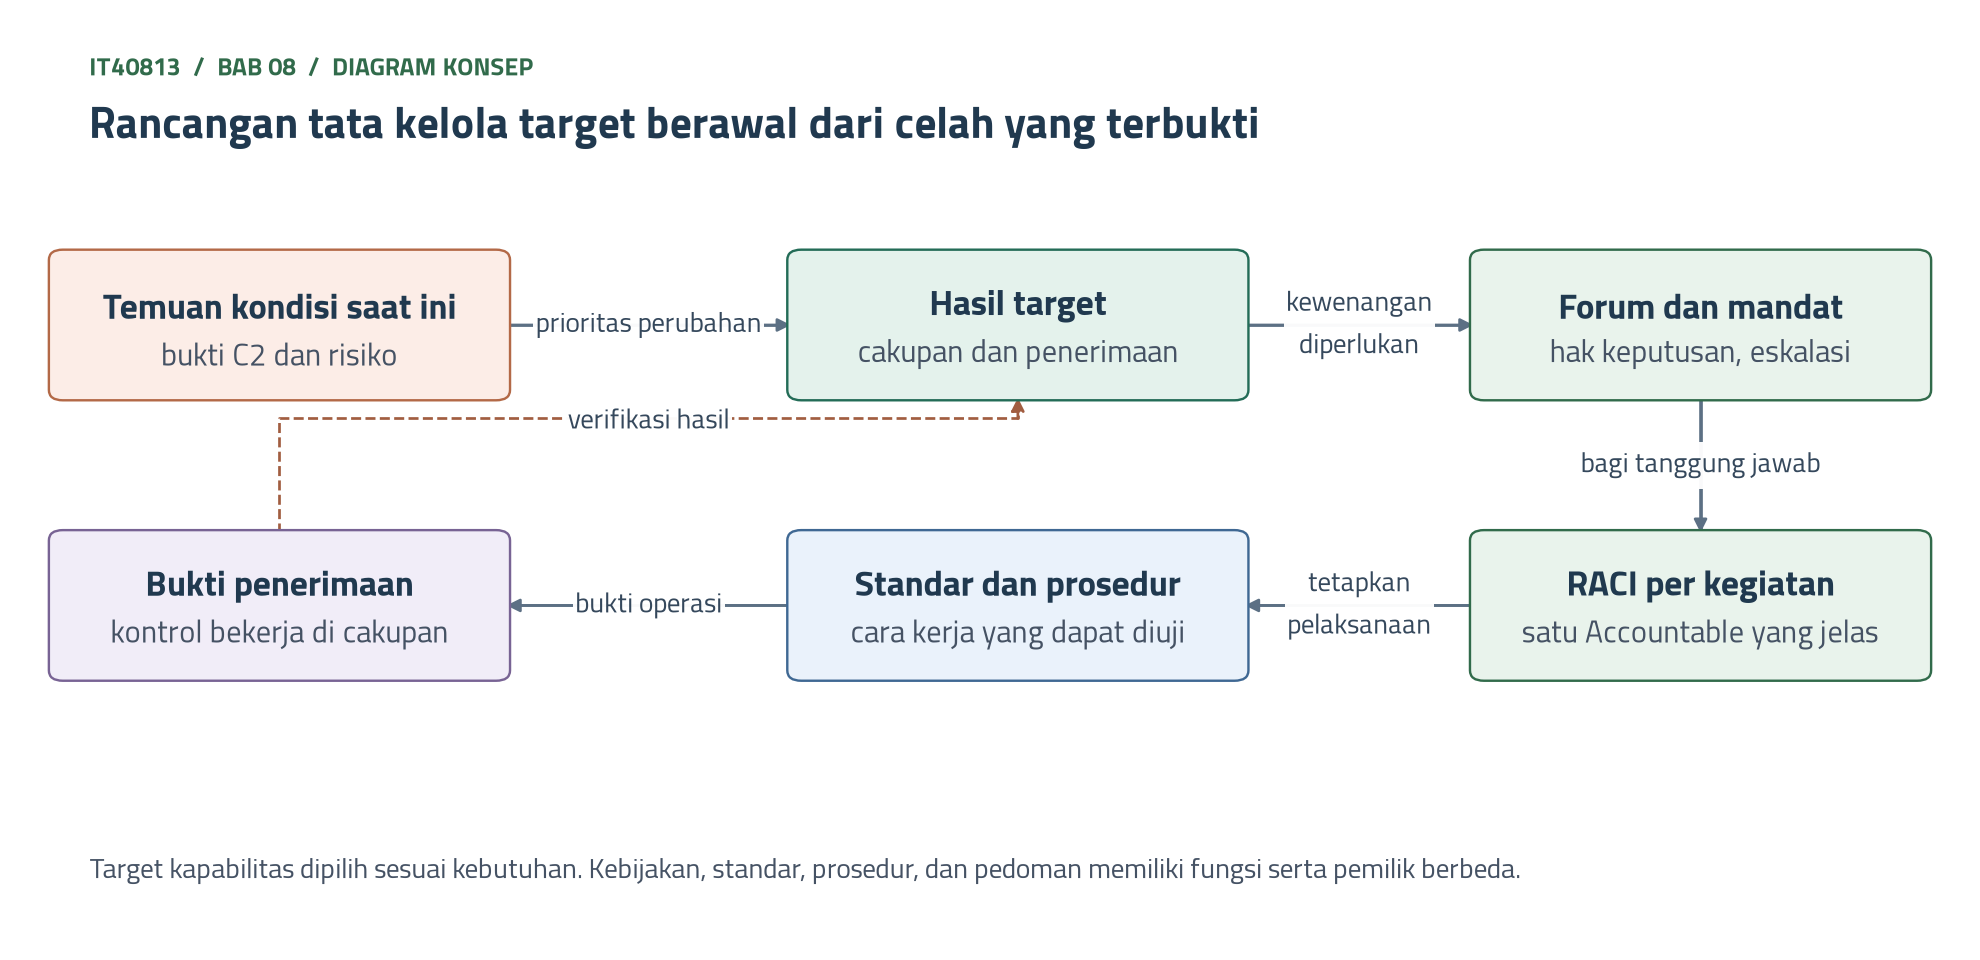
\includegraphics[width=\textwidth]{../figures/ch08-diagram-konsep.png}
  \caption{Rancangan tata kelola target berawal dari celah yang terbukti}
  \label{fig:ch08-ilustrasi-bab}
\end{figure}
}{}

\section{Dari Temuan C2 ke Keputusan Target}

\subsection*{Empat tahap panduan desain}

Desain target menjelaskan hasil yang ingin dicapai dan cara mempertanggungjawabkannya. Panduan
desain COBIT 2019 memuat empat tahap: memahami konteks dan strategi, menetapkan cakupan awal,
menyempurnakan cakupan, lalu menyelesaikan konflik dan menyimpulkan rancangan
\cite{c08-isaca-press}. Tahap akhir memberi tiap objektif terpilih tingkat kapabilitas target
\cite{c04-kapabilitas}. Rancangan ini berulang. Bila konteks, strategi, atau faktor desain
berubah, rancangan ditinjau lagi \cite{c08-grijp2019}.

Analogi renovasi rumah memperjelas urutannya. Penghuni menetapkan kebutuhan, memeriksa kondisi,
memilih perubahan, lalu menyepakati rancangan serta biaya. Mengganti seluruh bagian dengan bahan
termahal tidak selalu menyelesaikan masalah utama.

Dua contoh menghubungkan target dengan bukti:
\begin{enumerate}
  \item Misalkan AC-01 baru punya bukti pada 1 dari 5 rumah sakit, atau 12 dari 60 catatan
  peninjauan per tahun. Target awal adalah peninjauan bulanan dengan bukti pencabutan pada
  seluruh lokasi, yaitu 60 dari 60 catatan, bukan langsung otomatisasi penuh. Perluasan itu
  berbiaya Rp60 juta per tahun pada hitungan Bab 5.
  \item Misalkan laporan 18 klinik tidak konsisten karena definisi indikator berbeda. Bila tiap
  klinik memerlukan 2 jam rekonsiliasi per bulan, pekerjaannya 432 jam per tahun, atau Rp25,92
  juta pada tarif Rp60.000 per jam dari Bab 7. Target menetapkan pemilik definisi dan aturan
  rekonsiliasi. Mengganti aplikasi lembar kerja tanpa definisi yang sama hanya menghasilkan
  angka berbeda lebih cepat.
\end{enumerate}

Gambar~\ref{fig:ch08-desain} menempatkan keempat tahap pada urutan capstone. Bab 4 memakai
faktor desain untuk memilih enam objektif awal, tetapi berhenti pada kondisi saat ini. Bab ini
mengerjakan tahap keempat.

\begin{figure}[!htb]
  \centering
  \begin{tikzpicture}[
  font=\scriptsize,
  tahap/.style={draw, rounded corners, align=center, text width=2.4cm,
    minimum height=1.05cm, fill=blue!8},
  capstone/.style={draw, rounded corners, align=center, minimum height=1.2cm},
  panah/.style={-{Stealth[length=2mm]}, thick},
  tautan/.style={dashed, -{Stealth[length=2mm]}}]
  \node[anchor=south west, font=\scriptsize\bfseries] at (-1.3,0.55)
    {Panduan desain COBIT 2019};
  \node[tahap] (t1) at (0,0) {1. Konteks\\dan strategi};
  \node[tahap] (t2) at (3,0) {2. Cakupan awal};
  \node[tahap] (t3) at (6,0) {3. Penyempurnaan\\cakupan};
  \node[tahap, fill=orange!12] (t4) at (9,0) {4. Kesimpulan\\rancangan};
  \draw[panah] (t1) -- (t2);
  \draw[panah] (t2) -- (t3);
  \draw[panah] (t3) -- (t4);
  \node[anchor=south west, font=\scriptsize\bfseries] at (0.15,-1.3) {Capstone Medikara};
  \node[capstone, fill=blue!8, text width=2.4cm] (c1) at (0,-2.2)
    {C1: strategi,\\hak keputusan,\\kewajiban};
  \node[capstone, fill=blue!8, text width=5.4cm] (c2) at (4.5,-2.2)
    {C2: Bab 4 memilih 6 objektif awal;\\Bab 5 sampai 7: risiko dan 13 celah};
  \node[capstone, fill=green!10, text width=2.4cm] (c3) at (9,-2.2)
    {C3: target, forum,\\RACI, kebijakan};
  \draw[tautan] (t1.south) -- (c1.north);
  \draw[tautan] (t2.south) -- (t2.south |- c2.north);
  \draw[tautan] (t3.south) -- (t3.south |- c2.north);
  \draw[tautan] (t4.south) -- (c3.north);
\end{tikzpicture}

  \caption{Empat tahap panduan desain dan penerapannya pada capstone}
  \label{fig:ch08-desain}
\end{figure}

Diagram konsep pada awal bab meringkas urutan kerja yang sama. Temuan kondisi saat ini memberi
prioritas perubahan. Prioritas menjadi hasil target beserta cakupan dan syarat penerimaannya.
Hasil target menentukan kewenangan yang diperlukan, sehingga forum dan mandat dirancang
sesudahnya. Forum membagi tanggung jawab ke dalam matriks \textit{Responsible, Accountable,
Consulted, Informed} (RACI) per kegiatan. RACI menetapkan pelaksanaan lewat standar dan
prosedur. Standar dan prosedur menghasilkan bukti operasi, lalu bukti penerimaan memverifikasi
hasil target. Seksi berikut mengikuti urutan itu.

\subsection*{Dari 13 celah menjadi empat paket}

Pertanyaan kemudian muncul: bagaimana memilih target ketika anggaran terbatas? Tim membandingkan
dampak celah terhadap batas risiko Bab 5, kewajiban hukum, ketergantungan, dan bukti hasil. Tim
juga mencatat inisiatif yang ditunda serta akibat penundaannya.

Bab 6 menghasilkan G-01 sampai G-06, dan Bab 7 menghasilkan CP-01 sampai CP-07, sehingga ada 13
celah. Masing-masing bab memilih tiga prioritas, yaitu G-01, G-03, dan G-05, serta CP-04, CP-01,
dan CP-05. Enam prioritas itu saling bertaut. CP-01 dan G-01 sama-sama menyentuh akun vendor.
CP-04 dan G-05 sama-sama menyentuh insiden bersama vendor. Tabel~\ref{tab:ch08-paket}
menyatukannya menjadi empat paket target. Seluruh target merupakan pengandaian.

\begin{table}[!htb]
  \centering\small
  \caption{Empat paket target dari celah prioritas C2 (misalkan)}\label{tab:ch08-paket}
  \begin{tabularx}{\textwidth}{|>{\raggedright\arraybackslash}p{0.13\textwidth}|>{\raggedright\arraybackslash}p{0.09\textwidth}|>{\raggedright\arraybackslash}p{0.12\textwidth}|>{\raggedright\arraybackslash}X|>{\raggedright\arraybackslash}X|}
    \hline
    \textbf{Paket} & \textbf{Celah} & \textbf{Risiko, kewajiban} & \textbf{Hasil target} &
    \textbf{Bukti penerimaan} \\ \hline
    A. Akses vendor & G-01, CP-01 & R-01, K-01, K-05 & Peninjauan bulanan pada 5 rumah sakit;
    perjanjian vendor lengkap & 120 dari 120 akun cocok; 60 dari 60 catatan AC-01; 11 dari 11
    butir perjanjian \\ \hline
    B. Pemulihan & G-03 & R-05, K-02 & Uji pemulihan terjadwal pada 36 fasilitas & 144 uji per
    tahun; hasil disahkan pemilik layanan \\ \hline
    C. Insiden dan pemberitahuan & G-05, CP-04 & R-01, R-12, K-04, K-05 & Prosedur bersama
    vendor dilatih & 2 latihan per tahun; laporan vendor dalam 12 jam; naskah siap sebelum jam
    ke-60 \\ \hline
    D. Jejak aktivitas & CP-05, G-02 & R-01, R-12, K-01 & Catatan rinci disimpan 90 hari dan
    ditinjau & Uji telusur satu rekam; 247 dari 260 tinjauan mingguan \\ \hline
  \end{tabularx}
\end{table}

Tujuh celah sisanya tidak dihapus. G-02 ikut Paket D. CP-06 selesai lewat rancangan peran pada
bab ini. CP-03 menjadi syarat alur berbagi data asuransi. G-04, G-06, CP-02, dan CP-07 tetap
tercatat dengan pemiliknya dan masuk gelombang kedua. R-11 tetap berada pada jalur pimpinan
klinis dengan direktur pelayanan sebagai pemilik risiko, seperti Bab 5.

Keputusan ini punya dua konsekuensi yang dapat dihitung. Pertama, beban kerjanya terukur. Bab 6
menghitung 576 jam per tahun untuk G-01 dan G-03. Bab 7 menghitung 96 jam per tahun untuk
latihan pemberitahuan. Misalkan satu tinjauan catatan aktivitas memerlukan 2 jam, sehingga 260
tinjauan memakan 520 jam. Totalnya 1.192 jam per tahun, atau sekitar 0,62 orang penuh waktu pada
1.920 jam kerja per tahun. Dengan tarif Rp60.000 per jam, nilainya Rp71,52 juta. Angka itu hanya
waktu staf, dan sebagian sudah termasuk dalam Rp60 juta untuk AC-01 pada Bab 5, sehingga kedua
angka tidak dijumlahkan begitu saja. Kedua, penundaan punya akibat. G-04 dan G-06 berkaitan
dengan R-02 berskor 12, sehingga R-02 tetap terbuka selama gelombang pertama. Pemilik Sistem
Informasi Manajemen Rumah Sakit (SIMRS) perlu mengetahui penundaan itu dan menyetujuinya secara
tertulis.

\section{Menetapkan Target Kapabilitas COBIT}

\subsection*{Target tidak sama dengan tingkat tertinggi}

Target kapabilitas menyatakan tingkat yang dituju untuk proses pada objektif terpilih. Bab 4
sudah menjelaskan maknanya. Tingkat 2 mencapai tujuan lewat aktivitas dasar yang lengkap.
Tingkat 3 memakai cara kerja dan aset organisasi. Tingkat 4 mengukur kinerja secara kuantitatif.
Tingkat 5 memakai pengukuran untuk perbaikan berkelanjutan \cite{c04-kapabilitas}. Tingkat lebih
tinggi menuntut lebih banyak aset, pengukuran, dan orang, sehingga tingkat tertinggi bukan
tujuan yang berlaku untuk seluruh proses.

Menurut Souza Neto dan rekan, contoh pada panduan desain memberi tingkat 4 untuk skor 75 atau
lebih, tingkat 3 untuk skor 50 atau lebih, tingkat 2 untuk skor 25 atau lebih, dan tingkat 1
untuk sisanya. Skor 75 pada contoh itu berarti kepentingan objektif sedikitnya 75 persen lebih
tinggi daripada situasi pembanding. Mereka mengkritik satu akibatnya: semua proses pada objektif
berskor sama menerima satu tingkat yang sama \cite{c04-kapabilitas}.

Analogi kendaraan rumah sakit menjelaskan pilihan itu. Ambulans diperiksa setiap hari dengan
catatan terukur. Mobil pengantar berkas cukup diservis berkala. Menyamakan keduanya menghabiskan
biaya tanpa menaikkan keselamatan.

Dua contoh memperlihatkan kesalahan yang sering muncul:
\begin{enumerate}
  \item Misalkan analis mengubah skor lokal DSS05 pada Bab 4, yaitu 12 dari 15, menjadi 80
  persen, lalu memakai ambang 75 sehingga DSS05 mendapat tingkat 4. Hitungan itu salah skala.
  Skor lokal Bab 4 adalah pengandaian dengan nilai maksimum 15. Ambang 75 berasal dari skor
  kepentingan relatif pada contoh panduan, dan hanya berlaku pada logika contoh tersebut.
  \item Bab 4 membaca studi di rumah sakit Denpasar. Naskah itu menyebut 5 objektif bernilai 75
  dan memerlukan tingkat 4, tetapi tabel targetnya mencantumkan tingkat 3 untuk APO12 dan DSS04
  \cite{c04-denpasar}. Selisih pada 2 dari 5 objektif mungkin beralasan. Alasan itu perlu
  tertulis, karena target tanpa alasan tidak dapat diuji ulang.
\end{enumerate}

\subsection*{Target Medikara}

Tabel~\ref{tab:ch08-target-kapabilitas} menetapkan target 12 bulan untuk enam objektif awal dan
BAI06 sebagai dependensi. Kolom bukti C2 bukan tingkat kapabilitas. Selain AC-01 pada DSS05, Bab
4 belum memberi penilaian kapabilitas, sehingga semua target ditandai sementara sampai penilaian
lengkap tersedia. SoA pada tabel berarti \textit{Statement of Applicability} dari Bab 6.
Gambar~\ref{fig:ch08-target-bertingkat} memperlihatkan bentuknya. Tiga objektif yang berkaitan
langsung dengan insiden 2025 dituju pada tingkat 3. Empat objektif lain cukup tingkat 2 pada
tahun pertama.

\begin{table}[!htb]
  \centering\small
  \caption{Target kapabilitas Medikara untuk 12 bulan (misalkan)}
  \label{tab:ch08-target-kapabilitas}
  \begin{tabularx}{\textwidth}{|>{\raggedright\arraybackslash}p{0.1\textwidth}|>{\raggedright\arraybackslash}p{0.06\textwidth}|>{\raggedright\arraybackslash}X|>{\raggedright\arraybackslash}p{0.08\textwidth}|>{\raggedright\arraybackslash}X|}
    \hline
    \textbf{Objektif} & \textbf{Skor} & \textbf{Bukti C2} & \textbf{Target} & \textbf{Alasan dan
    bukti penerimaan} \\ \hline
    DSS05 & 12 & AC-01 indikatif 1, hanya satu rumah sakit & 3 & Insiden 2025 dan K-01; satu
    prosedur berjalan di 5 rumah sakit \\ \hline
    APO10 & 12 & Perjanjian vendor memuat 6 dari 11 butir & 3 & K-05 tidak memenuhi; 11 dari 11
    butir dan latihan laporan 12 jam \\ \hline
    APO13 & 11 & SoA: 87 kontrol diperlukan, 6 dikecualikan & 3 & Kebijakan dan SoA ditinjau
    berkala; bukti pada 5 rumah sakit \\ \hline
    APO14 & 11 & 2.400 dari 96.000 data tidak cocok di Bogor & 2 & Data tunggal menunggu
    rancangan IT40613; definisi punya pemilik \\ \hline
    APO12 & 10 & 12 skenario sudah berpemilik & 2 & Perlu data dua triwulan lebih dahulu; 12
    skenario ditinjau tiap triwulan \\ \hline
    MEA03 & 10 & 7 dari 16 kewajiban belum diverifikasi & 2 & 16 dari 16 baris register
    terverifikasi \\ \hline
    BAI06 & 9 & 8 dari 10 tiket contoh lengkap & 2 & Dependensi perubahan; 10 dari 10 tiket
    contoh lengkap, termasuk darurat \\ \hline
  \end{tabularx}
\end{table}

\begin{figure}[!htb]
  \centering
  \begin{tikzpicture}[
  font=\scriptsize,
  x=1.75cm,
  y=0.62cm,
  batang3/.style={draw, fill=orange!12},
  batang2/.style={draw, fill=blue!8}]
  \foreach \tingkat in {0,1,2,3} {
    \draw[gray!35] (\tingkat,0.6) -- (\tingkat,-6.6);
    \node[above] at (\tingkat,0.6) {\tingkat};
  }
  \fill[red!22] (3.96,0.6) rectangle (4.04,-6.6);
  \node[above] at (4,0.6) {4};
  \node[fill=red!22, align=center, rounded corners, text width=1.75cm] at (4.62,-3)
    {Usulan\\semua\\tingkat 4};
  \node[above, font=\scriptsize\bfseries] at (2,1.25) {Tingkat kapabilitas target};
  \node[anchor=east] at (-0.08,0) {DSS05, skor 12};
  \node[anchor=east] at (-0.08,-1) {APO10, skor 12};
  \node[anchor=east] at (-0.08,-2) {APO13, skor 11};
  \node[anchor=east] at (-0.08,-3) {APO14, skor 11};
  \node[anchor=east] at (-0.08,-4) {APO12, skor 10};
  \node[anchor=east] at (-0.08,-5) {MEA03, skor 10};
  \node[anchor=east] at (-0.08,-6) {BAI06, skor 9};
  \draw[batang3] (0,-0.35) rectangle (3,0.35);
  \draw[batang3] (0,-1.35) rectangle (3,-0.65);
  \draw[batang3] (0,-2.35) rectangle (3,-1.65);
  \draw[batang2] (0,-3.35) rectangle (2,-2.65);
  \draw[batang2] (0,-4.35) rectangle (2,-3.65);
  \draw[batang2] (0,-5.35) rectangle (2,-4.65);
  \draw[batang2] (0,-6.35) rectangle (2,-5.65);
  \fill (1,0) circle (1.6pt);
  \node[anchor=west] at (1.05,0) {AC-01 indikatif 1};
  \node[anchor=north west, align=left, text width=10cm] at (-1.05,-6.8)
    {{\tiny\mdseries Bulatan: AC-01 pada satu rumah sakit, bukan tingkat DSS05. Biaya per objektif
    per tahun (pengandaian): tingkat 2 Rp60 juta, tingkat 3 Rp120 juta, tingkat 4 Rp300 juta.
    Target ditandai sementara sampai penilaian kapabilitas lengkap tersedia.}};
\end{tikzpicture}

  \caption{Target kapabilitas bertingkat dibanding usulan tingkat 4 (misalkan)}
  \label{fig:ch08-target-bertingkat}
\end{figure}

Dua objektif sengaja tidak mendapat target pada tabel itu. DSS04 menunggu analisis dampak bisnis
pada Bab 10, tetapi 144 uji pemulihan pada Paket B tetap berjalan. APO09 berskor 7 tetap
ditunda, walaupun praktik tingkat layanan tetap dipakai pada seksi ITIL. Penundaan target tidak
menghentikan pekerjaan yang sudah diwajibkan.

\begin{kasus}[title={Kasus Medikara Health: Usulan Tingkat 4 untuk Semua Objektif}]
Misalkan konsultan mengusulkan tingkat 4 untuk ketujuh objektif, dengan alasan angka terukur
mudah dilaporkan. Misalkan pula biaya per objektif per tahun Rp60 juta untuk tingkat 2, Rp120
juta untuk tingkat 3, dan Rp300 juta untuk tingkat 4. Pada DSS05, angka Rp120 juta sudah
mencakup AC-01 sebesar Rp60 juta. Usulan konsultan menelan 7 kali Rp300 juta, atau Rp2,1 miliar
per tahun. Rancangan bertingkat menelan 3 kali Rp120 juta ditambah 4 kali Rp60 juta, atau Rp600
juta. Selisihnya Rp1,5 miliar per tahun.

Keputusan ini punya tiga konsekuensi. Pertama, pada DSS05 saja, kenaikan dari tingkat 3 ke
tingkat 4 menambah Rp180 juta. Setelah AC-01, peluang R-01 menjadi 0,05 dengan kerugian
rata-rata Rp500 juta, sehingga harapan kerugiannya Rp25 juta per tahun. Sekalipun tingkat 4
menghapus seluruh sisa risiko itu, manfaatnya hanya Rp25 juta. Kedua, peluang kerugian Rp1,5
miliar atau lebih pada R-01 sudah 1 persen, di dalam batas 2 persen pada Bab 5. Ketiga, Rp600
juta melewati batas Rp400 juta, sehingga keputusan tetap naik ke direksi, bukan berhenti di
komite pengarah TI.

Hitungan rupiah bukan satu-satunya pertimbangan. Keselamatan pasien dan hak pasien tidak diukur
dengan harapan kerugian saja. Target ditinjau lagi bila AC-01 gagal pada tiga peninjauan
berturut-turut, bila ada kewajiban baru, atau bila arsitektur target berubah.

Rp600 juta adalah rancangan awal untuk tujuh objektif. Setelah analisis dampak bisnis selesai, Bab
10 menambahkan DSS04 pada tingkat 3 dengan kode T-24. Rancangannya menjadi 4 kali Rp120 juta
ditambah 4 kali Rp60 juta, atau Rp720 juta per tahun, dan keputusan tetap berada di direksi. Bab 14
memakai angka Rp720 juta.
\end{kasus}

Hitungan batas risiko dapat dipakai dengan arah sebaliknya. Misalkan kerugian Rp2 miliar pada
R-05 terjadi setiap kali pemulihan gagal. Dengan peluang 0,1, peluang kerugian Rp1,5 miliar atau
lebih adalah 10 persen, jauh di atas batas 2 persen. Peluangnya harus turun menjadi seperlima.
Karena itu, Paket B tidak dapat dipangkas walaupun skor R-05 lebih rendah daripada R-01.

\begin{pendalaman}
Souza Neto dan rekan mengusulkan penyempurnaan. Target ditetapkan satu tingkat demi satu tingkat,
dari tingkat 2 sampai tingkat 5. Tiap aktivitas diberi peringkat N, P, L, atau F, dengan
\textit{Not} di bawah 15 persen, \textit{Partially} 15 sampai 50 persen, \textit{Largely} 50
sampai 85 persen, dan \textit{Fully} lebih dari 85 persen. Proses naik hanya bila aktivitas pada
tingkat itu berperingkat L atau F. Mereka juga memetakan keluaran proses berskor rendah ke proses
berskor tinggi. MEA02 mendapat tingkat 2 pada contoh panduan, tetapi mengirim keluaran ke enam
objektif berskor tertinggi, sehingga tingkat rendah tidak patut diberikan otomatis
\cite{c04-kapabilitas}.

Metode ini usulan penulis, bukan aturan asesmen ISACA. Biaya penilaiannya dapat dihitung dari
asumsi Bab 4. Tujuh objektif dengan rata-rata 35 aktivitas berarti 245 aktivitas, atau 122,5 jam
pada 30 menit per aktivitas. Pada Medikara, BAI06 berskor paling rendah, tetapi Bab 4 menunjukkan
perubahan di rumah sakit Bogor ikut merusak data pada APO14. Keterkaitan seperti itu dapat
menjadi alasan menaikkan target BAI06 pada tahun kedua.
\end{pendalaman}

\section{Profil Target NIST CSF}

\subsection*{Profil target menyebut hasil yang dipilih}

Bab 6 menyerahkan profil target kepada bab ini. Profil target menyebut hasil yang dipilih dan
diprioritaskan organisasi untuk mencapai sasaran pengelolaan risiko keamanannya. Profil itu juga
memperhitungkan perubahan yang diperkirakan, seperti persyaratan baru, adopsi teknologi baru,
dan tren ancaman. Selisih dengan profil saat ini dianalisis, lalu menjadi rencana tindakan
berprioritas \cite{nistcsf2}. Bab 6 mengerjakan langkah 1 sampai 4 untuk profil
saat ini dengan pembanding sementara. Bab ini mengisi kolom target pada langkah 3, menyelesaikan
analisis celah pada langkah 4, dan menyiapkan langkah 5.

Analogi pemeriksaan kesehatan berkala membantu. Hasil laboratorium menunjukkan keadaan saat ini.
Dokter menetapkan sasaran berbeda untuk gula darah, kolesterol, dan tekanan darah sesuai risiko
pasien. Tidak semua angka harus sempurna pada bulan yang sama.

Dua contoh menuntut ukuran hasil yang nyata:
\begin{enumerate}
  \item Misalkan target PR.AA-05 mencakup 5 rumah sakit dalam 6 bulan. Penerimaan memerlukan 30
  dari 30 catatan peninjauan selama 6 bulan itu, atau 60 dari 60 per tahun. Pelatihan
  administrator saja tidak cukup.
  \item Misalkan pembukaan data asuransi untuk 72.000 klaim per tahun membutuhkan inventaris
  alur, penilaian dampak, serta batas akses. Forum arsitektur memeriksa kesesuaiannya dengan
  rancangan platform IT40613 dan layanan cloud IT40713. NIST juga menyebut profil target dapat
  menyatakan persyaratan kepada pemasok dan mitra \cite{nistcsf2}. Karena itu, laporan 12 jam
  dan 11 butir perjanjian dapat masuk kontrak vendor pada Bab 9.
\end{enumerate}

Tabel~\ref{tab:ch08-profil-target} menyusun profil target Medikara. Empat belas baris pertama
berasal dari profil saat ini Bab 6, dengan cakupan 5 rumah sakit dan Medikara+. Dua baris
terakhir, GV.PO-01 dan GV.PO-02, ditambahkan karena bab ini menata kebijakan. NIST merumuskan
keduanya sebagai kebijakan pengelolaan risiko keamanan yang ditetapkan, dikomunikasikan,
ditegakkan, dan ditinjau \cite{nistcsf2}. Keduanya belum pernah dinilai, sehingga profil menjadi
16 dari 106 subkategori dan kolom saat ini harus diisi lebih dahulu. Pada tabel, Multi-Factor
Authentication (MFA) mengikuti Bab 6, dan Gel. 2 berarti gelombang kedua.

\begin{table}[!htb]
  \centering\footnotesize
  \caption{Profil target NIST CSF Medikara untuk 12 bulan (misalkan)}
  \label{tab:ch08-profil-target}
  \begin{tabularx}{\textwidth}{|>{\raggedright\arraybackslash}p{0.13\textwidth}|>{\raggedright\arraybackslash}p{0.13\textwidth}|>{\raggedright\arraybackslash}p{0.11\textwidth}|>{\raggedright\arraybackslash}X|>{\raggedright\arraybackslash}p{0.07\textwidth}|}
    \hline
    \textbf{Subkategori} & \textbf{Saat ini} & \textbf{Target} & \textbf{Bukti penerimaan} &
    \textbf{Paket} \\ \hline
    GV.OC-03 & Sebagian & Terbukti & 16 dari 16 baris register terverifikasi & Umum \\ \hline
    GV.RM-02 & Sebagian & Terbukti & Batas diuji dengan satu penyimpangan & Umum \\ \hline
    GV.RR-02 & Sebagian & Terbukti & Mandat dan RACI disahkan; 120 akun berpemilik & A \\ \hline
    GV.SC-07 & Sebagian & Terbukti & Tinjauan vendor berkala; 11 dari 11 butir & A, C \\ \hline
    ID.AM-02 & Sebagian & Sebagian & Rekonsiliasi berjalan pada 2 dari 5 rumah sakit & Gel. 2 \\
    \hline
    PR.AA-01 & Sebagian & Sebagian & Nol akun bersama pada sampel 2 rumah sakit & Gel. 2 \\
    \hline
    PR.AA-03 & Sebagian & Terbukti & MFA pada 120 dari 120 akun & A \\ \hline
    PR.AA-05 & Sebagian & Terbukti & 120 dari 120 akun cocok; 60 dari 60 catatan & A \\ \hline
    PR.AA-06 & Tidak relevan & Tidak relevan & Ditinjau bila vendor hadir di lokasi & Umum \\
    \hline
    PR.PS-04 & Terbukti & Terbukti & Cakupan ditambah Medikara+; catatan rinci 90 hari & D \\
    \hline
    PR.DS-11 & Sebagian & Terbukti & Cadangan disertai hasil uji pemulihan & B \\ \hline
    DE.CM-03 & Sebagian & Terbukti & 247 dari 260 tinjauan mingguan & D \\ \hline
    RS.MA-01 & Belum ada bukti & Terbukti & 2 latihan bersama; laporan vendor dalam 12 jam & C \\
    \hline
    RC.RP-03 & Belum ada bukti & Terbukti & 144 uji per tahun; hasil disahkan & B \\ \hline
    GV.PO-01 & Belum dinilai & Terbukti & KB-01 dan KB-05 disahkan serta disosialisasikan & Umum
    \\ \hline
    GV.PO-02 & Belum dinilai & Terbukti & 8 dari 8 dokumen ditinjau sesuai jadwal & Umum \\
    \hline
  \end{tabularx}
\end{table}

Pembacaan tabel memberi dua hal. Pada 14 baris Bab 6, status terbukti naik dari 1 menjadi 11,
sebagian turun dari 10 menjadi 2, dan belum ada bukti turun dari 2 menjadi 0. Satu baris tetap
tidak relevan. Selain itu, ID.AM-02 dan PR.AA-01 sengaja tetap sebagian, karena G-06 dan G-04
masuk gelombang kedua. Profil target yang semua barisnya terbukti pada tahun pertama sering
menandakan pilihan belum dibuat.

Perubahan yang diperkirakan juga masuk rancangan. Bab 7 mencatat Peraturan Pemerintah (PP)
33/2026 berlaku 16 Januari 2027, tetapi naskah resminya belum diperoleh, sehingga aturan itu
tetap menjadi butir pemantauan \cite{bpom-pp33-2026-status}. Rencana modernisasi ke cloud pada
IT40713 dapat mengubah cakupan PR.DS-11 dan RC.RP-03. Bila arsitektur berubah, baris yang
terkena ditinjau ulang.

\subsection*{Tier tidak dihitung dari profil}

Dua hal pada profil target sering tertukar: target hasil dan \textit{tier}. Pembagiannya begini.
Target hasil menyebut apa yang harus tercapai. \textit{Tier} menggambarkan ketelitian pengelolaan
risiko. NIST mendorong kenaikan \textit{tier} bila risiko atau mandat lebih besar, atau bila
analisis biaya dan manfaat menunjukkan penurunan risiko yang layak \cite{nistcsf2}.

Tabel~\ref{tab:ch08-tiga-target} melanjutkan batas pada Bab 6. Ketiga ukuran tidak saling
dikonversi. Medikara menuju Tier 3 untuk Protect karena R-01 dan K-01 merupakan risiko dan mandat
yang besar. Pada Bab 6, Tier 3 berarti praktik disetujui resmi sebagai kebijakan dan diperbarui
berkala, sehingga arsitektur kebijakan pada bab ini menjadi syaratnya. Tier 4 memerlukan
informasi pemasok yang hampir waktu nyata. Medikara belum menjadikannya target, karena biayanya
belum dapat dibenarkan pada tahun pertama.

\begin{table}[!htb]
  \centering\small
  \caption{Tiga target yang tidak saling dikonversi (misalkan)}\label{tab:ch08-tiga-target}
  \begin{tabularx}{\textwidth}{|>{\raggedright\arraybackslash}p{0.22\textwidth}|>{\raggedright\arraybackslash}X|>{\raggedright\arraybackslash}X|}
    \hline
    \textbf{Ukuran} & \textbf{Saat ini} & \textbf{Target} \\ \hline
    Status lokal PR.AA-05 & Sebagian, bukti 1 dari 5 rumah sakit & Terbukti pada 5 rumah sakit \\
    \hline
    \textit{Tier} Protect & Tier 2 pada pembacaan pimpinan & Tier 3 pada pembacaan pimpinan \\
    \hline
    Tingkat kapabilitas DSS05 & Indikatif 1 lewat AC-01 pada satu rumah sakit & Tingkat 3 setelah
    penilaian lengkap \\ \hline
  \end{tabularx}
\end{table}

\section{Struktur, Forum Keputusan, dan Pemisahan Tugas}

\subsection*{Forum dan peran kunci}

Hasil target menentukan kewenangan yang diperlukan. Struktur tata kelola membagi hak keputusan
dan pengawasan. Forum harus memiliki mandat, anggota, kuorum, jenis keputusan, jalur eskalasi,
serta catatan hasil. ISO/IEC 38500:2024 memakai tugas evaluasi, pengarahan, dan pemantauan, lalu
menambahkan pelibatan pemangku kepentingan \cite{c02-iso-perubahan}. Peterson memandang struktur,
proses, dan hubungan kerja sebagai satu kesatuan \cite{c02-peterson2004}. Forum tanpa proses
hanya menambah rapat.

Beberapa peran kunci perlu dibedakan. Chief Information Security Officer (CISO), yang pada mata
kuliah lain disebut kepala keamanan informasi, mengoordinasikan keamanan. Petugas pelindungan data memberi penilaian sesuai tugas dan independensinya. Pemilik
data menetapkan aturan pemakaian data. Pemilik layanan bertanggung jawab atas hasil layanan.
Forum arsitektur (\textit{architecture board}) memeriksa kesesuaian rancangan dengan prinsip
arsitektur. Rincian forum arsitektur dibahas pada mata kuliah IT40513.

Analogi rapat pengelola gedung menunjukkan perlunya mandat. Petugas perawatan dapat memperbaiki
lampu. Ia tidak otomatis berwenang mengubah jalur evakuasi atau menerima risiko keselamatan
penghuni.

Dua contoh menghindari persetujuan yang berputar:
\begin{enumerate}
  \item Misalkan usulan data asuransi berjalan berurutan melewati 4 forum bulanan. Waktu
  tunggunya paling lama 4 bulan. Dengan 5 menit per klaim, 6.000 klaim manual memakan 500 jam per
  bulan, atau Rp30 juta per bulan. Empat bulan berarti Rp120 juta. Alur pada
  Gambar~\ref{fig:ch08-alur-data} selesai dalam 10 hari kerja, sekitar setengah bulan atau Rp15
  juta. Selisihnya Rp105 juta, dan tinjauan hukum, privasi, keamanan, serta arsitektur tetap ada.
  \item Misalkan Medikara mencatat 40 perubahan per bulan: 30 kecil, 8 biasa, dan 2 darurat. Bila
  semuanya dibawa ke komite pengarah TI selama 5 menit per usulan, diperlukan 200 menit. Bab 2
  menyediakan rapat 120 menit per bulan. Perubahan kecil tampilan janji temu yang tidak mengubah
  data atau kendali keamanan memakai persetujuan terdelegasi bila kriteria dan bukti pengujiannya
  terpenuhi.
\end{enumerate}

Tabel~\ref{tab:ch08-forum} merangkum rancangan forum dan peran. Komite pengarah TI dan batas
delegasi mengikuti Bab 2. Keanggotaan komite risiko dan forum arsitektur merupakan pengandaian
bab ini. Komite risiko beranggotakan direktur keuangan sebagai ketua, direktur pelayanan, kepala
risiko, hukum, dan CISO. Pada tabel, Data Protection Impact Assessment (DPIA) mengikuti Bab 7.
Gambar~\ref{fig:ch08-peta-peran} menempatkan semuanya pada Three Lines Model dari Bab 1.

\begin{table}[!htb]
  \centering\small
  \caption{Rancangan forum dan peran Medikara (misalkan)}\label{tab:ch08-forum}
  \begin{tabularx}{\textwidth}{|>{\raggedright\arraybackslash}p{0.2\textwidth}|>{\raggedright\arraybackslash}X|>{\raggedright\arraybackslash}X|>{\raggedright\arraybackslash}p{0.2\textwidth}|}
    \hline
    \textbf{Forum atau peran} & \textbf{Mandat} & \textbf{Aturan kerja} & \textbf{Bukti hasil} \\
    \hline
    Direksi & Risiko di atas batas; keputusan di atas Rp400 juta sampai Rp5 miliar & Laporan
    triwulan ke dewan komisaris & Keputusan, alasan, batas waktu \\ \hline
    Komite pengarah TI & Prioritas dan anggaran lintas fasilitas sampai Rp400 juta & 9 anggota,
    kuorum 6; bulanan 2 jam & Notulen dan pemilik manfaat \\ \hline
    Komite risiko & Menelaah risiko di atas batas; memberi rekomendasi ke direksi & 5 anggota,
    kuorum 4; triwulanan 2 jam & Rekomendasi dan pemantauan batas \\ \hline
    Forum arsitektur & Kesesuaian rancangan dan pengecualian standar & 6 anggota; dua kali sebulan
    1 jam; kepala TI memutuskan & Catatan keputusan arsitektur \\ \hline
    Direktur pelayanan & Akuntabilitas rekam medis terpadu dan tujuan berbagi data & Naik ke
    direksi bila melewati batas & Keputusan tujuan dan mutu layanan \\ \hline
    Kepala rekam medis & Pemilik data; aturan data rekam medis & Hak henti bila dasar pemrosesan
    belum ada & Catatan henti dan alasan \\ \hline
    Pemilik layanan & Hasil layanan, akses teknis, uji pemulihan & Pengecualian darurat paling
    lama 24 jam & Catatan AC-01, hasil uji \\ \hline
    CISO & Koordinasi keamanan dan tinjauan standar & Lini kedua; tidak menyetujui akses & Pendapat
    dan temuan tertulis \\ \hline
    Petugas pelindungan data & Pendapat DPIA dan pemantauan pemrosesan & 1 penuh waktu, 5
    koordinator 20 persen & Pendapat DPIA \\ \hline
  \end{tabularx}
\end{table}

\begin{figure}[!htb]
  \centering
  \begin{tikzpicture}[
  font=\scriptsize,
  kotak/.style={draw, rounded corners, align=center, text width=3cm, minimum height=1.1cm},
  panah/.style={-{Stealth[length=2mm]}, thick}]
  \node[draw, rounded corners, align=center, text width=10.5cm, minimum height=0.9cm,
    fill=praditagreen!15] (bp) at (0,0)
    {\textbf{Badan pengarah}\\Dewan komisaris mengawasi; direksi memutuskan sesuai kewenangan};
  \node[kotak, fill=blue!8] (fa) at (-3.75,-1.75)
    {\textbf{Forum arsitektur}\\standar dan pola integrasi};
  \node[kotak, fill=blue!8] (kp) at (0,-1.75)
    {\textbf{Komite pengarah TI}\\9 anggota, sampai Rp400 juta};
  \node[kotak, fill=blue!8] (kr) at (3.75,-1.75)
    {\textbf{Komite risiko}\\5 anggota, rekomendasi risiko};
  \node[kotak, fill=orange!12, minimum height=1.5cm] (l1) at (-3.75,-3.85)
    {\textbf{Lini pertama}\\direktur pelayanan, pemilik layanan, kepala rekam medis, operasi TI};
  \node[kotak, fill=blue!8, minimum height=1.5cm] (l2) at (0,-3.85)
    {\textbf{Lini kedua}\\CISO, petugas pelindungan data, kepala risiko, hukum};
  \node[kotak, fill=green!10, minimum height=1.5cm] (l3) at (3.75,-3.85)
    {\textbf{Lini ketiga}\\audit internal, asurans independen};
  \draw[panah] (fa) -- (kp);
  \draw[panah] (kp) -- (kp |- bp.south);
  \draw[panah] (kr) -- (kr |- bp.south);
  \draw[panah] (l1) -- (fa);
  \draw[panah] (l1.north east) -- (kp.south west);
  \draw[panah] (l2.north east) -- (kr.south west);
  \draw[panah] (l2.south) -- ++(0,-0.3) -| (l1.south)
    node[pos=0.25, below] {{\tiny\mdseries memantau dan menantang}};
  \draw[panah] (l3.east) -- ++(0.28,0) |- (bp.east);
\end{tikzpicture}

  \caption{Forum dan peran pada Three Lines Model (misalkan)}
  \label{fig:ch08-peta-peran}
\end{figure}

Penunjukan petugas pelindungan data menutup CP-06. Bab 7 mengandaikan kapasitasnya setara 2 orang
penuh waktu, dan kepala TI tidak merangkap peran itu. CISO berada pada lini kedua. Three Lines
Model membedakan peran, bukan departemen \cite{iia-tlm2026}, sehingga bila fungsi keamanan juga
menjalankan tinjauan catatan aktivitas pada G-02, peran pelaksana dan peran penantang perlu
dipegang orang berbeda.

Pertanyaan berikutnya: apakah Medikara perlu komite risiko terpisah? Biaya forum dapat dihitung.
Komite pengarah TI memakan $9 \times 2 \times 12 = 216$ jam orang per tahun. Komite risiko
memakan $5 \times 2 \times 4 = 40$ jam. Forum arsitektur memakan $6 \times 1 \times 24 = 144$ jam.
Jumlahnya 400 jam, atau sekitar Rp24 juta pada tarif Rp60.000 per jam. Biaya sesungguhnya lebih
tinggi karena tarif pimpinan lebih mahal. Pilihan lain adalah agenda risiko triwulanan pada
komite pengarah TI, yang menghemat 40 jam tetapi menambah agenda pada rapat 2 jam yang sudah
padat. Misalkan Medikara memilih komite terpisah karena R-11 dan K-04 memerlukan pembahasan yang
tidak bercampur dengan anggaran. Organisasi kecil dapat memilih sebaliknya. Yang dinilai adalah
kemampuan forum mengambil keputusan, bukan banyaknya forum.

\begin{kasus}[title={Kasus Medikara Health: Dua Pertanyaan C3}]
Pertanyaan pertama: siapa menyetujui pembukaan data kepada mitra? Misalkan direktur pelayanan
memutuskan tujuan berbagi data. Pemilik layanan mengusulkan tujuan dan data minimum. Petugas
pelindungan data menyusun pendapat atas DPIA, yang pada Bab 7 memerlukan 72 jam dalam 3 hari
kerja. Hukum, keamanan, dan forum arsitektur meninjau secara paralel selama 5 hari kerja. Kepala
rekam medis memegang hak henti sempit bila dasar pemrosesan belum ada. Risiko sisa di atas batas
naik ke direksi. Gambar~\ref{fig:ch08-alur-data} merangkum alurnya.

Pertanyaan kedua: siapa memegang akuntabilitas atas rekam medis terpadu? Misalkan direktur
pelayanan memegangnya. Peran itu sejalan dengan Bab 2, yang menempatkannya sebagai pemilik manfaat
layanan, dan Bab 5, yang menempatkannya sebagai pemilik R-11. Kepala rekam medis menjalankan aturan
data. Kepala TI menjalankan platform, tetapi tidak memegang akuntabilitas hasil klinis.

Rancangan ini punya tiga konsekuensi. Pertama, jalur tinjauan menjadi lebih pendek. Tinjauan
berurutan oleh hukum, keamanan, dan arsitektur memakan 15 hari kerja, sehingga seluruh alur
menjadi 20 hari kerja. Tinjauan paralel membuatnya 10 hari kerja. Kedua, peluang lolos naik. Bab 2
menghitung empat veto dengan persetujuan 90 persen menghasilkan 65,6 persen. Dengan satu hak henti
sempit, angka itu menjadi 90 persen, dan masukan pihak lain wajib didengar serta dijawab tertulis.
Ketiga, mandat internal tidak menghapus aturan. Bab 3 mencatat Permenkes 24/2022 Pasal 30: hak
akses ditetapkan pimpinan fasilitas \cite{permenkes24-2022}. Model menyediakan aturan yang sama,
tetapi penetapan pada 36 fasilitas tetap harus ada. Tafsir hukum atas susunan ini perlu
dikonfirmasi kepada fungsi hukum.
\end{kasus}

\begin{figure}[!htb]
  \centering
  \begin{tikzpicture}[
  font=\scriptsize,
  tahap/.style={draw, rounded corners, align=center, text width=2.4cm,
    minimum height=1.3cm, fill=blue!8},
  panah/.style={-{Stealth[length=2mm]}, thick}]
  \node[tahap] (n1) at (0,0)
    {Usulan tujuan dan data minimum\\{\tiny\mdseries pemilik layanan, hari 1}};
  \node[tahap] (n2) at (3,0)
    {DPIA\\{\tiny\mdseries petugas pelindungan data, hari 2 sampai 4}};
  \node[tahap] (n3) at (6,0)
    {Tinjauan paralel\\{\tiny\mdseries hukum, keamanan, arsitektur, hari 5 sampai 9}};
  \node[tahap, fill=orange!12] (n4) at (9,0)
    {Keputusan tujuan\\{\tiny\mdseries direktur pelayanan, hari 10}};
  \node[tahap, fill=red!22] (h1) at (3,-2.1)
    {Dasar pemrosesan belum ada\\{\tiny\mdseries kepala rekam medis menghentikan}};
  \node[tahap, fill=gray!35] (h2) at (6,-2.1)
    {Risiko sisa di atas batas\\{\tiny\mdseries naik ke direksi}};
  \node[tahap, fill=green!10] (h3) at (9,-2.1)
    {Akses teknis mitra\\{\tiny\mdseries pemilik layanan, operasi TI}};
  \draw[panah] (n1) -- (n2);
  \draw[panah] (n2) -- (n3);
  \draw[panah] (n3) -- (n4);
  \draw[panah] (n2) -- (h1);
  \draw[panah] (n4) -- (h2);
  \draw[panah] (n4) -- (h3);
\end{tikzpicture}

  \caption{Alur persetujuan pembukaan data kepada mitra dalam 10 hari kerja (misalkan)}
  \label{fig:ch08-alur-data}
\end{figure}

\subsection*{Pemisahan tugas}

Pemisahan tugas membatasi pihak yang mengusulkan, menyetujui, menjalankan, dan menguji. NIST
menyebut pemisahan tugas sebagai salah satu kontrol akses \cite{c08-nist-sp80012r1}. Tujuannya
sederhana: tidak ada satu orang yang dapat membuat masalah sekaligus menutupinya.

Analogi kas kecil kantor menjelaskan alasannya. Orang yang mengeluarkan uang tidak mencocokkan
buku kasnya sendiri. Pencocokan oleh orang lain membuat selisih lebih cepat terlihat.

Dua contoh memperlihatkan penerapannya:
\begin{enumerate}
  \item Tabel~\ref{tab:ch08-pemisahan} menerapkan empat tugas pada AC-01. Administrator tidak
  menyetujui aksesnya sendiri. Audit internal menguji secara independen, dan contoh pada Bab 6
  memakai 30 akun sampel, dengan 24 akun sesuai.
  \item Misalkan satu klinik hanya memiliki 1 administrator. Pemisahan penuh tidak mungkin,
  sehingga Medikara memakai pemeriksaan kompensasi oleh peninjau pusat. Pada 18 klinik, peninjauan
  bulanan 15 menit per klinik memakan 54 jam per tahun. Potensi konflik dan bukti tinjauannya
  tetap dicatat.
\end{enumerate}

\begin{table}[!htb]
  \centering\small
  \caption{Pemisahan tugas pada AC-01 (misalkan)}\label{tab:ch08-pemisahan}
  \begin{tabularx}{\textwidth}{|>{\raggedright\arraybackslash}p{0.18\textwidth}|>{\raggedright\arraybackslash}p{0.27\textwidth}|>{\raggedright\arraybackslash}X|}
    \hline
    \textbf{Tugas} & \textbf{Pemegang} & \textbf{Bukti} \\ \hline
    Mengusulkan & Pengelola vendor & Daftar penugasan dan tanggal berakhir \\ \hline
    Menyetujui & Pemilik Medikara+ & Persetujuan per akun \\ \hline
    Menjalankan & Operasi TI & Tiket pemberian dan pencabutan \\ \hline
    Menguji & Audit internal & Hasil uji sampel dan temuan \\ \hline
  \end{tabularx}
\end{table}

\section{Matriks RACI yang Dapat Dipakai}

RACI membedakan pelaksana, pemegang akuntabilitas, pihak yang dimintai pertimbangan, dan pihak
yang diberi informasi. Dalam rancangan kelas ini setiap baris memiliki satu \textit{Accountable}
agar keputusan akhir jelas. Satu orang boleh menjalankan beberapa peran bila kewenangan dan
pemisahan tugas tetap dapat dipertanggungjawabkan.

Analogi pengelolaan acara memperjelas pembagian. Banyak panitia menjalankan kegiatan, tetapi satu
penanggung jawab menetapkan keputusan akhir untuk satu kegiatan. Bila dua pihak sama-sama
menganggap yang lain memutuskan, pekerjaan berhenti.

Dua contoh menunjukkan perlunya unit keputusan yang tepat:
\begin{enumerate}
  \item Misalkan baris berjudul ``mengelola seluruh data'' diberi dua \textit{Accountable}, yaitu
  TI dan pimpinan klinis. Tim memecahnya menjadi aturan rekam medis, tujuan berbagi data, akses
  teknis, dan uji pemulihan. Satu baris kabur menjadi 4 baris dengan pemegang akuntabilitas yang
  jelas.
  \item Bab 2 menempatkan pemberian akses vendor pada D-06, dengan pemilik Medikara+ sebagai
  pemutus dan eskalasi ke direktur pelayanan bila kepala TI keberatan. Model target menulisnya
  sebagai satu \textit{Accountable}, yaitu pemilik layanan, dan operasi TI sebagai
  \textit{Responsible}. Keamanan memberi pertimbangan. Administrator tidak menyetujui aksesnya
  sendiri.
\end{enumerate}

Dua hal sering tertukar: \textit{Accountable} dan \textit{Responsible}. Pembagiannya begini.
\textit{Responsible} mengerjakan. \textit{Accountable} menanggung keputusan akhir dan menjawab
bila hasilnya gagal. Kepala operasi TI dapat menjalankan 144 uji pemulihan, sedangkan pemilik
layanan yang mengesahkan apakah layanannya benar-benar pulih.

Tabel~\ref{tab:ch08-raci} merangkum 10 keputusan dengan 9 peran. Salinannya tersedia di
\berkas{sources/chapter08/contoh-raci-medikara.csv}. Audit internal sengaja tidak masuk matriks,
karena peran lini ketiga menguji hasil kerja dan tidak ikut memutuskan.

\begin{table}[!htb]
  \centering\small
  \caption{Contoh RACI keputusan target Medikara (misalkan)}\label{tab:ch08-raci}
  \begin{tabularx}{\textwidth}{|>{\raggedright\arraybackslash}X|*{9}{>{\centering\arraybackslash}p{0.042\textwidth}|}}
    \hline
    \textbf{Keputusan} & \textbf{Dir} & \textbf{DP} & \textbf{PL} & \textbf{RM} & \textbf{TI} &
    \textbf{KA} & \textbf{PD} & \textbf{HK} & \textbf{FA} \\ \hline
    1. Aturan rekam medis terpadu & I & A & C & R & C & C & C & C & C \\ \hline
    2. Tujuan berbagi data mitra & I & A & R & C & I & C & C & C & C \\ \hline
    3. Akses teknis mitra & - & I & A & C & R & C & I & I & C \\ \hline
    4. Peninjauan akses AC-01 & I & I & A & - & R & C & I & - & - \\ \hline
    5. Pencabutan akun vendor & - & - & A & - & R & C & I & - & - \\ \hline
    6. Perubahan darurat SIMRS & I & C & A & C & R & C & I & - & I \\ \hline
    7. Penerimaan risiko di atas batas & A & C & R & C & C & C & C & C & I \\ \hline
    8. Uji pemulihan & I & I & A & C & R & C & - & - & I \\ \hline
    9. Pemberitahuan insiden data & I & C & C & C & C & R & R & A & - \\ \hline
    10. Subprosesor dan penghentian vendor & I & C & A & C & R & C & C & C & C \\ \hline
  \end{tabularx}

  \vspace{4pt}
  {\footnotesize Dir direksi; DP direktur pelayanan; PL pemilik layanan; RM kepala rekam medis;
  TI operasi TI; KA keamanan (CISO); PD petugas pelindungan data; HK hukum; FA forum arsitektur.}
\end{table}

Matriks itu dapat dibaca seperti data. Huruf A berjumlah 10, dan tiap baris mempunyai tepat satu
A. Pemilik layanan memegang 6 dari 10 A. Angka itu aman hanya bila peran tersebut dipegang
beberapa orang, misalnya pemilik Medikara+ dan pemilik SIMRS, dengan pengganti yang ditunjuk.
Keamanan muncul sebagai C pada 9 dari 10 baris. Misalkan tiap baris terjadi 4 kali per bulan dan
satu pertimbangan memerlukan 2 jam. Bebannya $9 \times 4 \times 2 = 72$ jam per bulan, atau 45
persen dari 160 jam kerja. Kolom C terbanyak menjadi antrean. Bila baris 4 dan 5 memakai kriteria
tetap sehingga keamanan cukup menjadi I, bebannya turun menjadi 56 jam, atau 35 persen.

RACI tidak menggantikan wewenang dalam piagam atau aturan hukum. Kolom C juga bukan hak veto
universal. Jika dua fungsi mempunyai persetujuan terpisah yang wajib, tim membuat baris keputusan
masing-masing dan menjelaskan ketergantungannya. Baris 2 dan baris 3 pada tabel adalah contohnya:
tujuan disetujui lebih dahulu, baru akses teknis diberikan.

Tiga bacaan memberi gambaran pemakaiannya. Feltus dan rekan mengajukan model tanggung jawab
karyawan yang dibangun atas kewajiban, hak, dan komitmen, membandingkannya dengan konsep pada COBIT,
lalu mengilustrasikan usulan perubahannya pada bagan RACI \cite{c08-feltus2009}. Michałek
merancang matriks RACI untuk organisasi proyek matriks dengan pendekatan \textit{design science research}, menerapkannya pada
tiga portofolio proyek pada 2023, lalu memvalidasi serta menyempurnakannya pada 2024
\cite{c08-michalek2026}. Hartono dan rekan memakai RACI untuk membagi kegiatan mitigasi setelah
analisis risiko pada satu usaha \cite{c08-hartono2024}. Abstrak ketiga sumber itu tidak
melaporkan angka hasil. Karena itu, bab ini memperlakukan aturan satu \textit{Accountable} sebagai
aturan rancangan yang perlu diuji lewat simulasi, bukan temuan yang berlaku umum.

\section{Arsitektur dan Siklus Hidup Kebijakan}

\subsection*{Empat jenis dokumen}

Kebijakan menyatakan arah dan tanggung jawab pada tingkat yang luas. NIST menjelaskan bahwa
organisasi karena itu menyusun standar, pedoman, dan prosedur agar pelaksanaannya lebih jelas.
Standar biasanya wajib di dalam organisasi. Pedoman membantu pelaksana dan dapat dijalankan dengan
lebih dari satu cara. Prosedur merinci langkah untuk menjalankan kebijakan, standar, dan pedoman
\cite{c08-nist-sp80012r1}. Setiap dokumen memiliki pemilik, versi, persetujuan, tanggal berlaku,
pelatihan, dan jadwal tinjau.

Analogi aturan perpustakaan memisahkan tingkatnya. Kebijakan menetapkan pelindungan koleksi.
Standar menetapkan lama peminjaman. Pedoman membantu petugas menghadapi kasus khusus. Prosedur
menjelaskan pencatatan dan pengembalian.

Dua contoh menunjukkan akibat dokumen yang tidak terhubung:
\begin{enumerate}
  \item Misalkan kebijakan mewajibkan akses sesuai tugas, tetapi prosedur keluar vendor tidak
  meminta pencabutan akun. Bab 6 menghitung pencabutan turun dari 24 menjadi 9, 5, dan 2 akun
  setelah prosedur itu diubah. Kalimat kebijakan tidak berubah sama sekali. Yang berubah adalah
  tautannya dengan langkah kerja.
  \item Misalkan standar masa simpan catatan rinci diusulkan menjadi 180 hari. Bab 7 sudah
  menghitung kenaikan dari 7 menjadi 90 hari menaikkan ruang simpan 12,9 kali. Angka 180 hari
  menaikkannya 25,7 kali dari 7 hari, dan menggandakan paparan data pribadi dibanding 90 hari. Tim
  menilai dasar serta tujuan sebelum menyetujui angka. Retensi rekam medis 25 tahun pada K-03
  tidak disalin ke semua jenis catatan.
\end{enumerate}

Gambar~\ref{fig:ch08-hierarki} memperlihatkan hubungannya. Standar dan pedoman ditempatkan sejajar,
karena keduanya menurunkan kebijakan dengan sifat yang berbeda. Tabel~\ref{tab:ch08-kebijakan}
menerapkan keempatnya pada akses vendor. NIST juga menyarankan pemisahan yang jelas antara
kebijakan dan pelaksanaannya, karena pemisahan itu memberi keleluasaan cara pelaksanaan
\cite{c08-nist-sp80012r1}.

\begin{figure}[!htb]
  \centering
  \begin{tikzpicture}[
  font=\scriptsize,
  lapis/.style={draw, rounded corners, align=center, minimum height=0.95cm},
  catatan/.style={anchor=west, align=left, text width=4.5cm},
  panah/.style={-{Stealth[length=2mm]}, thick}]
  \node[lapis, fill=praditagreen!15, text width=5.8cm] (kb) at (0,0)
    {\textbf{Kebijakan}\\arah dan tanggung jawab};
  \node[lapis, fill=blue!8, text width=2.7cm] (st) at (-1.55,-1.45)
    {\textbf{Standar}\\ketentuan wajib};
  \node[lapis, fill=blue!8, text width=2.7cm] (pd) at (1.55,-1.45)
    {\textbf{Pedoman}\\pilihan pelaksanaan};
  \node[lapis, fill=orange!12, text width=5.8cm] (pr) at (0,-2.9)
    {\textbf{Prosedur}\\langkah kerja yang dapat diuji};
  \node[lapis, fill=green!10, text width=5.8cm] (bk) at (0,-4.35)
    {\textbf{Bukti operasi}\\catatan AC-01, tiket pencabutan, hasil uji};
  \draw[panah] (kb.south -| st) -- (st);
  \draw[panah] (kb.south -| pd) -- (pd);
  \draw[panah] (st) -- (pr.north -| st);
  \draw[panah] (pd) -- (pr.north -| pd);
  \draw[panah] (pr) -- (bk);
  \node[catatan] at (3.35,0) {KB-01, KB-05\\Disetujui direksi; tinjau 24 bulan};
  \node[catatan] at (3.35,-1.45)
    {KB-02, KB-06 disetujui komite pengarah TI; KB-04 disetujui direktur pelayanan; tinjau
    12 bulan};
  \node[catatan] at (3.35,-2.9)
    {KB-03, KB-07, KB-08\\Disetujui kepala TI atau komite; tinjau 12 bulan};
  \node[catatan] at (3.35,-4.35) {Diperiksa terhadap bukti penerimaan};
\end{tikzpicture}

  \caption{Arsitektur kebijakan dan penyetujunya (misalkan)}
  \label{fig:ch08-hierarki}
\end{figure}

\begin{table}[!htb]
  \centering\small
  \caption{Hubungan jenis dokumen dan bukti pada akses vendor (misalkan)}
  \label{tab:ch08-kebijakan}
  \begin{tabularx}{\textwidth}{|>{\raggedright\arraybackslash}p{0.14\textwidth}|>{\raggedright\arraybackslash}X|>{\raggedright\arraybackslash}X|}
    \hline
    \textbf{Jenis} & \textbf{Isi akses vendor} & \textbf{Bukti} \\ \hline
    Kebijakan & Akses sesuai kebutuhan dan dapat ditelusuri & Persetujuan serta pemilik \\ \hline
    Standar & Akun pribadi, MFA, dan masa berlaku wajib & Daftar syarat pemeriksaan \\ \hline
    Pedoman & Contoh akses darurat terbatas & Contoh skenario dan pelatihan \\ \hline
    Prosedur & Beri, tinjau, dan cabut akun paling lambat 1 hari kerja & Catatan AC-01 dan tiket
    pencabutan \\ \hline
  \end{tabularx}
\end{table}

\subsection*{Daftar kebijakan dan bebannya}

Pertanyaan kemudian muncul: dokumen mana yang benar-benar perlu ditulis? Medikara tidak mulai dari
daftar dokumen ideal. Medikara mulai dari celah. Tabel~\ref{tab:ch08-daftar-kebijakan} menurunkan
delapan dokumen dari paket target. Kodenya KB, karena awalan K sudah dipakai register kewajiban
Bab 3.

\begin{table}[!htb]
  \centering\footnotesize
  \caption{Daftar kebijakan yang dibuat atau direvisi (misalkan)}
  \label{tab:ch08-daftar-kebijakan}
  \begin{tabularx}{\textwidth}{|>{\raggedright\arraybackslash}p{0.08\textwidth}|>{\raggedright\arraybackslash}p{0.11\textwidth}|>{\raggedright\arraybackslash}X|>{\raggedright\arraybackslash}p{0.11\textwidth}|>{\raggedright\arraybackslash}p{0.17\textwidth}|>{\raggedright\arraybackslash}p{0.17\textwidth}|}
    \hline
    \textbf{ID} & \textbf{Jenis} & \textbf{Nama} & \textbf{Celah} & \textbf{Pemilik} &
    \textbf{Penyetuju} \\ \hline
    KB-01 & Kebijakan & Akses dan penggunaan data & G-01, G-04 & Kepala rekam medis & Direksi \\
    \hline
    KB-02 & Standar & Akun vendor & G-01, CP-01 & CISO & Komite pengarah TI \\ \hline
    KB-03 & Prosedur & AC-01 dan pencabutan & G-01 & Pemilik layanan & Kepala TI \\ \hline
    KB-04 & Pedoman & Akses darurat klinis & R-05, R-11 & Pimpinan klinis & Direktur pelayanan \\
    \hline
    KB-05 & Kebijakan & Berbagi data dengan mitra & CP-03 & Direktur pelayanan & Direksi \\ \hline
    KB-06 & Standar & Masa simpan catatan aktivitas & CP-05, G-02 & CISO & Komite pengarah TI \\
    \hline
    KB-07 & Prosedur & Pemberitahuan insiden & CP-04, G-05 & Fungsi hukum & Komite pengarah TI \\
    \hline
    KB-08 & Prosedur & Uji pemulihan & G-03 & Pemilik layanan & Kepala TI \\ \hline
  \end{tabularx}
\end{table}

Keputusan ini punya dua konsekuensi. Pertama, bebannya terukur. Misalkan kebijakan ditinjau tiap
24 bulan dan dokumen lain tiap 12 bulan, sehingga ada 7 tinjauan per tahun. Dengan 8 jam per
tinjauan, bebannya 56 jam. Pelatihan 2 jam untuk 52 staf TI menambah 104 jam. Jumlahnya 160 jam,
atau satu bulan kerja, senilai Rp9,6 juta. Kedua, perubahan menjadi lebih ringan. Direksi hanya
menyetujui 2 dari 8 dokumen. Enam dokumen lain dapat berubah tanpa rapat direksi, selama arahnya
tetap sama.

\subsection*{Pengecualian}

Pengecualian harus menyebut ruang lingkup, risiko sisa, kontrol kompensasi, pemberi persetujuan,
dan kedaluwarsa. Tanpa masa berlaku, pengecualian sementara dapat menjadi kebijakan tanpa disadari.
Bab 5 sudah memberi contohnya. Vendor meminta 4 akun tetap aktif selama 10 hari, sehingga
paparannya 40 akun-hari. Pemilik Medikara+ memberi pengecualian darurat 24 jam, sehingga paparannya
4 akun-hari, atau turun 90 persen. Misalkan pengecualian yang berulang lebih dari tiga kali dibawa
ke pemilik standar, karena standarnya mungkin perlu diubah.

\section{COBIT dan ITIL 4 dalam Operasi Layanan}

COBIT membantu memilih hasil tata kelola dan manajemen serta menilai kapabilitas. ITIL 4 membantu
organisasi mengelola layanan lewat sistem nilai layanan (\textit{service value system}) dan
praktik kerja \cite{cobit2019-intro,itil4}. Praktik pada ITIL 4 adalah sekumpulan sumber daya
organisasi untuk melakukan pekerjaan atau mencapai sasaran. ITIL 4 terbit pada 2019 dengan panduan
terpisah untuk 34 praktik \cite{c08-griffith-praktik}. Modul PeopleCert menempatkan \textit{change
enablement}, \textit{incident management}, dan \textit{service level management} pada tiga
kelompok berbeda \cite{c08-peoplecert-modul}. Hubungan COBIT dan ITIL pada bab ini merupakan
pemetaan pembelajaran, bukan pernyataan kesetaraan resmi.

Analogi sekolah memisahkan pertanyaan arah dan pelaksanaan. Pengelola menetapkan hasil belajar
serta pertanggungjawaban. Guru menyusun cara mengajar dan mengelola kelas. Keduanya perlu terhubung
tanpa mengambil alih seluruh tugas pihak lain.

Dua contoh rumah sakit memperlihatkan perannya:
\begin{enumerate}
  \item Misalkan perubahan SIMRS harus mempertahankan keselamatan dan jejak persetujuan. Bab 4
  mengandaikan 8 dari 10 tiket lengkap, dan 2 tiket darurat tanpa analisis dampak. BAI06 memberi
  arah hasil dan pengawasan, sedangkan \textit{change enablement} membantu penilaian risiko,
  otorisasi, dan penjadwalan. Sepuluh tiket yang sama menjadi bukti bagi keduanya.
  \item Misalkan gangguan integrasi berlangsung 30 menit. Dengan 274 kunjungan per jam pada
  hitungan Bab 5, gangguan itu menyentuh 137 kunjungan dan memakai 25 persen batas 2 jam per bulan.
  \textit{Incident management} mengembalikan layanan. PeopleCert menganjurkan insiden dilihat dari
  sisi pemakai layanan \cite{c08-griffith-praktik}. Analisis masalah berulang dan peninjauan risiko
  kemudian mengubah cara pengendaliannya.
\end{enumerate}

Tabel~\ref{tab:ch08-itil} merangkum pemetaan pembelajaran objektif dan praktik. Nama objektif
mengikuti katalog Bab 4. Tingkat layanan pada baris APO09 memakai batas Bab 5: 2 jam gangguan dari
360 jam layanan per bulan, yaitu 12 jam per hari selama 30 hari, setara ketersediaan sekitar 99,44
persen.

\begin{table}[!htb]
  \centering\small
  \caption{Pemetaan pembelajaran objektif COBIT dan praktik ITIL 4 (misalkan)}\label{tab:ch08-itil}
  \begin{tabularx}{\textwidth}{|>{\raggedright\arraybackslash}p{0.26\textwidth}|>{\raggedright\arraybackslash}p{0.25\textwidth}|>{\raggedright\arraybackslash}X|}
    \hline
    \textbf{Objektif COBIT} & \textbf{Praktik ITIL 4} & \textbf{Bukti layanan} \\ \hline
    BAI06 \textit{Managed IT changes} & \textit{Change enablement} & Penilaian, otorisasi, uji, dan
    rencana pemulihan \\ \hline
    DSS02 \textit{Managed service requests and incidents} & \textit{Incident management} &
    Kronologi, pemulihan, komunikasi \\ \hline
    DSS03 \textit{Managed problems} & \textit{Problem management} & Akar masalah dan perbaikan
    permanen \\ \hline
    APO09 \textit{Managed service agreements} & \textit{Service level management} & Target 2 jam
    per bulan dan tinjauan hasil \\ \hline
    APO10 \textit{Managed vendors} & \textit{Supplier management} & Perjanjian, tinjauan, laporan
    12 jam \\ \hline
    APO13 \textit{Managed security} & \textit{Information security management} & Kebijakan, SoA,
    hasil tinjauan \\ \hline
  \end{tabularx}
\end{table}

Jenis perubahan perlu dibedakan agar komite tidak tenggelam. Pada 40 perubahan per bulan di atas,
30 perubahan kecil memakai kriteria standar dan disetujui lebih dahulu. Delapan perubahan biasa
dinilai oleh pemegang wewenang perubahan. Dua perubahan darurat memakai pengecualian 24 jam dan
ditinjau pada rapat berikutnya, sesuai Bab 2. Dalam setahun, 24 perubahan darurat itu layak
diperiksa sebagai pola. Bila jumlahnya naik, mungkin yang bermasalah adalah perencanaan rilis.

Tingkat layanan mitra juga dapat dibaca dengan cara yang sama. Bab 3 mengandaikan kontrak mitra
asuransi meminta pemberitahuan gangguan dalam 1 jam, dan hanya 2 dari 12 gangguan yang tepat waktu,
atau 16,7 persen. \textit{Service level management} menetapkan sasaran yang jelas dan berbasis
bisnis \cite{c08-peoplecert-modul}, sedangkan APO09 memeriksa apakah sasaran itu dipantau dan
dibahas.

PeopleCert juga menyediakan ITIL (Version 5). Halaman resminya menyebut versi ini hasil evolusi
yang dibangun di atas konsep kunci ITIL 4: prinsip panduan, sistem nilai layanan, rantai nilai,
praktik, dan perbaikan berkelanjutan. Perubahan utamanya mencakup model siklus hidup produk dan
layanan, rantai nilai yang disederhanakan, serta istilah dan definisi praktik yang baru
\cite{c08-itil5-foundation}. Modul ini menyebut ITIL 4 secara eksplisit agar istilah dan bahan
capstone konsisten. Perubahan versi perlu dicatat ketika sumber organisasi memakai versi lain, dan
praktik dari beberapa versi tidak dicampur tanpa penjelasan.

\section{Bukti Penerimaan dan Simulasi Keputusan}

Bukti penerimaan menyatakan kapan sebuah target dianggap tercapai. Bukti itu ditetapkan sebelum
pekerjaan dimulai, dan diperiksa oleh pihak yang bukan pelaksananya. Diagram konsep
menggambarkannya sebagai verifikasi hasil yang kembali ke hasil target. Bila bukti tidak memenuhi,
yang ditinjau adalah pelaksanaan, cakupan, atau targetnya.

Analogi serah terima renovasi menjelaskan bedanya. Penghuni tidak cukup menerima nota pembelian
keran. Penghuni memutar keran itu dan memeriksa airnya mengalir.

Dua contoh memisahkan kegiatan dari hasil:
\begin{enumerate}
  \item Misalkan 52 staf TI selesai dilatih tentang AC-01. Pelatihan itu kegiatan. Bukti
  penerimaannya adalah 120 dari 120 akun cocok, 60 dari 60 catatan, dan audit internal menemukan
  30 dari 30 akun sampel sesuai, dibanding 24 dari 30 pada kondisi saat ini.
  \item Bab 6 mencatat 150 pekerjaan cadangan berhasil dalam 30 hari. Angka itu bukan bukti
  pemulihan. Bukti penerimaan Paket B adalah 144 uji per tahun, data contoh pulih, dan hasilnya
  disahkan pemilik layanan.
\end{enumerate}

Tabel~\ref{tab:ch08-bukti} menetapkan pemeriksa dan akibat bila bukti gagal untuk keempat paket.

\begin{table}[!htb]
  \centering\small
  \caption{Pemeriksaan bukti penerimaan empat paket (misalkan)}\label{tab:ch08-bukti}
  \begin{tabularx}{\textwidth}{|>{\raggedright\arraybackslash}p{0.09\textwidth}|>{\raggedright\arraybackslash}X|>{\raggedright\arraybackslash}p{0.19\textwidth}|>{\raggedright\arraybackslash}X|}
    \hline
    \textbf{Paket} & \textbf{Bukti operasi} & \textbf{Pemeriksa} & \textbf{Bila gagal} \\ \hline
    A & Catatan AC-01 dan tiket pencabutan & Audit internal & Pemilik Medikara+ menyusun perbaikan;
    laporan ke komite risiko \\ \hline
    B & Hasil 144 uji pemulihan & Pemilik layanan, lalu audit internal & Uji ulang; R-05
    dilaporkan ke direksi \\ \hline
    C & Catatan 2 latihan bersama & Petugas pelindungan data & Prosedur KB-07 diubah; latihan
    diulang \\ \hline
    D & Uji telusur satu rekam dan 247 dari 260 tinjauan & CISO & KB-06 ditinjau; tugas peninjau
    diperjelas \\ \hline
  \end{tabularx}
\end{table}

\begin{kasus}[title={Kasus Medikara Health: Menguji Model dengan Dua Keputusan}]
Misalkan tim menguji model di atas meja dengan dua keputusan. Keputusan pertama adalah pembukaan
data asuransi. Alur selesai pada hari ke-10, tetapi simulasi menemukan bahwa pendapat DPIA tidak
punya tempat pada catatan keputusan. Tim menambah kolom itu pada
\berkas{sources/chapter08/model-tata-kelola-target.md}.

Keputusan kedua adalah perubahan darurat SIMRS yang menghentikan pendaftaran pada jam layanan,
ketika pemilik layanan sedang cuti dan tidak ada pengganti. Operasi TI menunggu persetujuan selama
3 jam. Batas Bab 5 adalah 2 jam per bulan, sehingga gangguan itu melampauinya. Dengan 274 kunjungan
per jam, gangguan 3 jam setara 822 kunjungan.

Simulasi ini punya dua konsekuensi. Pertama, RACI yang rapi belum menjamin keputusan dapat dibuat.
Tim menambah aturan pengganti yang ditunjuk pada baris 6. Kedua, kebuntuan ditemukan tanpa pasien
yang terkena. Biaya simulasi 8 orang selama 2 jam hanya 16 jam kerja, atau Rp960.000 pada tarif
Rp60.000 per jam.
\end{kasus}

\begin{pendalaman}
\textit{Policy as code} menerjemahkan sebagian aturan menjadi pemeriksaan otomatis. Open Policy
Agent adalah mesin kebijakan sumber terbuka yang memisahkan pengambilan keputusan kebijakan dari
penegakannya. Perangkat lunak mengirim masukan terstruktur, lalu menerima keputusan. Aturannya
ditulis dalam bahasa Rego, dan dokumentasinya menyebut pemakaian pada Kubernetes serta
\textit{pipeline} Continuous Integration / Continuous Delivery (CI/CD) \cite{c08-opa}.

Misalkan perubahan tanpa pengenal persetujuan ditolak \textit{pipeline}. Pemeriksaan dapat menilai
keberadaan pengenal, tetapi tidak membuktikan pertimbangan klinis yang mendasarinya. Titik
pemeriksaan dirancang bersama IT40713 tanpa menghilangkan keputusan manusia untuk pengecualian
berisiko. Bagian ini opsional, dan hanya dijalankan pada sistem milik tim atau sistem dengan izin
tertulis.
\end{pendalaman}

\section{Aktivitas: Model Tata Kelola Target}

\textbf{Tujuan.} Tim merancang model tata kelola target berdasarkan kondisi target yang dirancang
di tiga mata kuliah lain. Isinya forum keputusan dan perannya, RACI untuk 8 sampai 10 keputusan,
target kapabilitas untuk objektif prioritas, profil target NIST CSF, dan daftar kebijakan. Tim
memakai organisasi nyata dengan izin dan data yang dianonimkan, atau kasus Medikara Health. Untuk
Medikara, model harus menjawab dua pertanyaan: siapa menyetujui pembukaan data ke mitra, dan siapa
memegang akuntabilitas atas rekam medis terpadu.

\textbf{Pembagian peran.} Pemilik konteks dan analis regulasi merancang struktur serta mandat.
Analis risiko menyelaraskan target dengan \textit{risk appetite}. Analis teknologi memetakan
praktik ITIL dan profil keamanan. Satu anggota berlatar nonteknis membaca seluruh rancangan sebagai
peninjau.

\textbf{Langkah kerja.}
\begin{enumerate}
  \item Baca celah C2, register risiko, serta rancangan target IT40513, IT40613, dan IT40713.
  Satukan celah prioritas menjadi tiga sampai lima paket.
  \item Isi \berkas{sources/chapter08/target-kapabilitas-csf.csv}. Tulis alasan tiap target, dan
  bedakan target kapabilitas dari hasil profil CSF.
  \item Isi \berkas{sources/chapter08/model-tata-kelola-target.md} untuk forum, delegasi, kuorum,
  eskalasi, dan catatan keputusan.
  \item Susun 8 sampai 10 baris dalam \berkas{sources/chapter08/raci.csv}. Uji satu
  \textit{Accountable} per baris, lalu bandingkan dengan
  \berkas{sources/chapter08/contoh-raci-medikara.csv}.
  \item Gunakan \berkas{sources/chapter08/daftar-kebijakan.csv} untuk dokumen yang dibuat atau
  direvisi beserta pengecualiannya.
  \item Petakan objektif prioritas dengan praktik ITIL 4, dan tandai sebagai pemetaan pembelajaran.
  \item Simulasikan persetujuan satu alur data mitra dan satu perubahan darurat. Catat waktu, lalu
  perbaiki baris yang menimbulkan kebuntuan.
\end{enumerate}

\textbf{Luaran.} Model tata kelola target yang memuat struktur, RACI, target kapabilitas, profil
target, daftar kebijakan, dan catatan dua simulasi.

\textbf{Kaitan dengan capstone.} Luaran masuk tonggak C3 Kondisi Target. Forum arsitektur
diselaraskan dengan IT40513. Alur data mitra diselaraskan dengan IT40613. Titik persetujuan
perubahan diselaraskan dengan IT40713. Target dipakai lagi pada Bab 9, Bab 10, dan Bab 11, lalu
diuji pada Bab 12 dan diukur pada Bab 13.

\textbf{Kriteria penilaian.} Keterlacakan celah 30 persen; kejelasan wewenang 30 persen; kelayakan
target 25 persen; bukti simulasi 15 persen. Struktur tidak dinilai dari banyaknya komite. Yang
dinilai adalah apakah keputusan dapat dibuat dan diuji.

\textbf{Berkas pendukung.} Seluruh lembar kerja ada di \berkas{sources/chapter08/}, dengan daftar
berkas pada \berkas{sources/chapter08/README.md}.

\textbf{Pendalaman teknis (opsional).} Tim dengan anggota berlatar teknis dapat mengenal
\textit{policy as code} memakai Open Policy Agent, lalu merancang alur persetujuan perubahan yang
menyatu dengan \textit{pipeline} CI/CD bersama IT40713.

\section{Ringkasan}

Desain target berangkat dari celah yang terbukti dan batas risiko. Panduan COBIT menyusunnya dalam
empat tahap, dan bab ini mengerjakan tahap terakhir. Tiga belas celah C2 disatukan menjadi empat
paket target, sementara celah sisanya tetap tercatat dengan pemilik. Target harus menyebut hasil,
cakupan, sumber daya, serta bukti penerimaan.

Tingkat kapabilitas tertinggi tidak otomatis paling tepat. Medikara menuju tingkat 3 pada tiga
objektif dan tingkat 2 pada empat objektif, dengan biaya pengandaian awal Rp600 juta per tahun,
bukan Rp2,1 miliar, dan Bab 10 menaikkannya menjadi Rp720 juta setelah DSS04 masuk sebagai T-24.
Profil target NIST CSF menaikkan status terbukti dari 1 menjadi 11 pada 14 baris Bab
6, dan menyisakan dua baris gelombang kedua secara sengaja. Status lokal, \textit{tier}, dan
tingkat kapabilitas tetap tidak saling dikonversi.

Struktur membagi mandat, keputusan, dan eskalasi. Direktur pelayanan memegang akuntabilitas rekam
medis terpadu dan memutuskan tujuan berbagi data, dengan hak henti sempit pada kepala rekam medis.
Pemisahan tugas mencegah persetujuan atas pekerjaan sendiri. RACI menerjemahkan pembagian itu
menjadi 10 keputusan dengan tepat satu pemegang akuntabilitas per baris, dan pembacaan kolomnya
menunjukkan antrean seperti beban keamanan 45 persen.

Kebijakan, standar, pedoman, dan prosedur membuat keputusan dapat dijalankan. Delapan dokumen KB
diturunkan dari celah, dan pengecualian memiliki batas waktu. COBIT, ITIL 4, dan NIST CSF membantu
pertanyaan yang berbeda, dan hubungannya dibuktikan lewat tiket serta hasil layanan yang sama.

Bukti penerimaan menutup lingkaran. Simulasi menemukan kebuntuan sebelum pasien terkena, dan
biayanya kecil. Pesan utama bab ini sederhana: tata kelola target berhasil ketika organisasi dapat
memutuskan, menjalankan, dan meninjau hasil secara konsisten, bukan ketika struktur dan dokumennya
terlihat lengkap.

\section{Latihan}

\subsection*{Latihan 1: Akuntabilitas RACI}

Mengapa dalam matriks RACI satu aktivitas hanya boleh memiliki satu pihak \textit{Accountable}?
Berikan contoh masalah bila aturan ini dilanggar. Latihan ini membuktikan bahwa dua pemegang
akuntabilitas pada satu baris dapat menghentikan keputusan.

\begin{enumerate}
  \item Pilih satu baris dengan dua \textit{Accountable} dari organisasi tim atau dari contoh.
  \item Catat keputusan yang berpotensi tertunda, lalu hitung akibatnya dalam waktu atau biaya.
  \item Pecah atau perbaiki baris sesuai wewenang.
  \item Uji baris baru dengan satu kejadian nyata atau simulasi.
\end{enumerate}

Tabel~\ref{tab:ch08-lat1-contoh} merangkum contoh analisis Latihan 1 dari skenario pembelajaran,
dan Tabel~\ref{tab:ch08-lat1-hasil} menyediakan lembar isiannya.

\begin{table}[!htb]
  \centering\small
  \caption{Contoh analisis Latihan 1 (skenario pembelajaran)}\label{tab:ch08-lat1-contoh}
  \begin{tabularx}{\textwidth}{|>{\raggedright\arraybackslash}X|>{\raggedright\arraybackslash}X|>{\raggedright\arraybackslash}X|}
    \hline
    \textbf{Baris (misalkan)} & \textbf{Masalah} & \textbf{Perbaikan} \\ \hline
    Setujui semua data: TI dan pimpinan klinis sama-sama A & Masing-masing menunggu; 3 bulan
    tertunda berarti 18.000 klaim manual, atau Rp90 juta & Pisah tujuan berbagi data (A direktur
    pelayanan) dari akses teknis (A pemilik layanan) \\ \hline
  \end{tabularx}
\end{table}

\begin{table}[!htb]
  \centering\small
  \caption{Lembar isian Latihan 1}\label{tab:ch08-lat1-hasil}
  \begin{tabularx}{\textwidth}{|>{\raggedright\arraybackslash}X|>{\raggedright\arraybackslash}X|>{\raggedright\arraybackslash}X|}
    \hline
    \textbf{Baris} & \textbf{Masalah} & \textbf{Perbaikan} \\ \hline
    \dots & \dots & \dots \\ \hline
    \dots & \dots & \dots \\ \hline
  \end{tabularx}
\end{table}

\textbf{Pertanyaan analisis.} Siapa menanggung akibat jika keputusan terlambat? Apakah pemecahan
baris tetap memenuhi persetujuan wajib? Pada Tabel~\ref{tab:ch08-raci}, pemilik layanan memegang 6
dari 10 A. Kapan angka itu menjadi masalah?

\subsection*{Latihan 2: COBIT dan ITIL}

Jelaskan perbedaan peran COBIT dan ITIL 4 dengan contoh proses manajemen perubahan di rumah sakit.
Latihan ini membuktikan bahwa satu tumpukan bukti dapat melayani dua kerangka tanpa membuat
keduanya setara.

\begin{enumerate}
  \item Pilih satu perubahan SIMRS beserta jenisnya: kecil, biasa, atau darurat.
  \item Tentukan hasil dan pengawasan yang dibutuhkan.
  \item Hubungkan praktik layanan dengan bukti pelaksanaan.
  \item Hitung bukti yang lengkap dari 10 tiket contoh.
\end{enumerate}

Tabel~\ref{tab:ch08-lat2-contoh} merangkum contoh analisis Latihan 2 dari skenario pembelajaran,
dan Tabel~\ref{tab:ch08-lat2-hasil} menyediakan lembar isiannya.

\begin{table}[!htb]
  \centering\small
  \caption{Contoh analisis Latihan 2 (skenario pembelajaran)}\label{tab:ch08-lat2-contoh}
  \begin{tabularx}{\textwidth}{|>{\raggedright\arraybackslash}X|>{\raggedright\arraybackslash}X|>{\raggedright\arraybackslash}X|}
    \hline
    \textbf{Kebutuhan} & \textbf{Peran kerangka} & \textbf{Bukti} \\ \hline
    Perubahan terkendali & COBIT BAI06 memberi arah hasil dan penilaian & 8 dari 10 tiket lengkap;
    angka itu kelengkapan sampel, bukan tingkat kapabilitas \\ \hline
    Perubahan dijalankan aman & ITIL 4 \textit{change enablement} membantu praktik & Otorisasi, uji,
    dan rencana pemulihan pada tiap tiket \\ \hline
  \end{tabularx}
\end{table}

\begin{table}[!htb]
  \centering\small
  \caption{Lembar isian Latihan 2}\label{tab:ch08-lat2-hasil}
  \begin{tabularx}{\textwidth}{|>{\raggedright\arraybackslash}X|>{\raggedright\arraybackslash}X|>{\raggedright\arraybackslash}X|}
    \hline
    \textbf{Kebutuhan} & \textbf{Peran kerangka} & \textbf{Bukti} \\ \hline
    \dots & \dots & \dots \\ \hline
    \dots & \dots & \dots \\ \hline
  \end{tabularx}
\end{table}

\textbf{Pertanyaan analisis.} Mengapa pemetaan tidak membuktikan kesetaraan? Celah apa tersisa bila
tiket lengkap tetapi pemulihan tidak diuji? Mengapa 2 tiket darurat yang gagal lebih berat daripada
2 tiket biasa?

\subsection*{Latihan 3: Target Tingkat 4}

Sebuah tim menetapkan target kapabilitas tingkat 4 untuk semua objektif. Kritisi keputusan ini dari
sisi biaya dan \textit{risk appetite}. Latihan ini membuktikan bahwa target harus dibenarkan oleh
risiko dan bukti, bukan oleh angkanya.

\begin{enumerate}
  \item Pilih tiga objektif dengan dampak berbeda.
  \item Bandingkan biaya tiap tingkat dengan harapan kerugian dan batas risiko terkait.
  \item Tetapkan target serta prioritas bertahap.
  \item Tulis pemicu yang akan membuat target dinaikkan.
\end{enumerate}

Tabel~\ref{tab:ch08-lat3-contoh} merangkum contoh analisis Latihan 3 dengan biaya pengandaian pada
seksi target kapabilitas, dan Tabel~\ref{tab:ch08-lat3-hasil} menyediakan lembar isiannya.

\begin{table}[!htb]
  \centering\small
  \caption{Contoh analisis Latihan 3 (skenario pembelajaran)}\label{tab:ch08-lat3-contoh}
  \begin{tabularx}{\textwidth}{|>{\raggedright\arraybackslash}p{0.11\textwidth}|>{\raggedright\arraybackslash}X|>{\raggedright\arraybackslash}p{0.09\textwidth}|>{\raggedright\arraybackslash}X|}
    \hline
    \textbf{Objektif} & \textbf{Usulan tingkat 4} & \textbf{Target} & \textbf{Analisis} \\ \hline
    DSS05 & Tambah Rp180 juta dari tingkat 3 & 3 & Sisa harapan kerugian R-01 hanya Rp25 juta;
    peluang 1 persen di dalam batas 2 persen \\ \hline
    APO12 & Tambah Rp240 juta dari tingkat 2 & 2 & Data dasar dua triwulan belum ada, sehingga
    ukuran kuantitatif belum bermakna \\ \hline
    BAI06 & Tambah Rp240 juta dari tingkat 2 & 2 & 8 dari 10 tiket lengkap; lengkapi dahulu 10 dari
    10 tiket \\ \hline
  \end{tabularx}
\end{table}

\begin{table}[!htb]
  \centering\small
  \caption{Lembar isian Latihan 3}\label{tab:ch08-lat3-hasil}
  \begin{tabularx}{\textwidth}{|>{\raggedright\arraybackslash}p{0.11\textwidth}|>{\raggedright\arraybackslash}X|>{\raggedright\arraybackslash}p{0.09\textwidth}|>{\raggedright\arraybackslash}X|}
    \hline
    \textbf{Objektif} & \textbf{Usulan tingkat 4} & \textbf{Target} & \textbf{Analisis} \\ \hline
    \dots & \dots & \dots & \dots \\ \hline
    \dots & \dots & \dots & \dots \\ \hline
  \end{tabularx}
\end{table}

\textbf{Pertanyaan analisis.} Apakah target tinggi menunda kontrol yang mendesak? Bukti apa
membenarkan biaya peningkatan berikutnya? Dengan biaya pengandaian bab ini, berapa selisih biaya
bila satu objektif lagi dinaikkan ke tingkat 3?

  % !TeX root = it-governance-risk-compliance.tex
% !TeX encoding = UTF-8
\chapter{Risiko Pihak Ketiga dan Cloud}

\section*{Tujuan Pembelajaran}
\begin{itemize}
  \item Menyusun siklus hidup manajemen risiko pihak ketiga, mulai dari uji tuntas sampai
  pemutusan kontrak.
  \item Memetakan pembagian tanggung jawab keamanan antara organisasi dan penyedia cloud.
  \item Menyusun penilaian dampak pelindungan data pribadi untuk alur berbagi data dengan mitra.
\end{itemize}

\section{Pendahuluan}

Kebocoran dapat terjadi di vendor, tetapi pasien tetap meminta pertanggungjawaban organisasi
yang melayaninya. Insiden Medikara pada 2025 memperlihatkan pola itu. Pada data latihan Bab 7,
kontrak pekerjaan vendor sudah selesai, tetapi akun dukungan tetap aktif. Selama 8 malam, akun
itu melakukan 155 panggilan per malam dan membaca 1.240 rekam kunjungan pada dua rumah sakit.
Medikara baru mengetahuinya pada hari ke-11 lewat keluhan pasien. Risiko pihak ketiga karena itu
tidak selesai ketika kontrak ditandatangani atau sertifikat penyedia diterima.

Strategi Medikara membuka kerja sama dengan klinik, asuransi, laboratorium, apotek daring, dan
penyedia cloud. Setiap hubungan mempunyai data, ketergantungan, serta hak keputusan berbeda.
Pemilihan mitra harus diikuti kendali selama hubungan berlangsung dan cara keluar yang dapat
diuji. Bab 8 sudah menetapkan targetnya: Paket A menuntut 11 dari 11 butir perjanjian vendor,
dan Paket C menuntut laporan vendor dalam 12 jam. Bab ini menjelaskan cara mencapainya. Hasil
kerjanya adalah kerangka pihak ketiga, matriks tanggung jawab cloud, dan penilaian dampak
pelindungan data pribadi, atau \textit{Data Protection Impact Assessment} (DPIA), untuk tonggak
C3 capstone.

Bab ini memakai ISO/IEC 27036-2:2022 dari International Organization for Standardization (ISO)
dan International Electrotechnical Commission (IEC) untuk hubungan pemasok. Panduan National
Institute of Standards and Technology (NIST) SP 800-161 Rev. 1 dipakai untuk risiko rantai
pasok, NIST SP 800-145 untuk definisi cloud, serta Cloud Controls Matrix (CCM) dan Consensus
Assessments Initiative Questionnaire (CAIQ) dari Cloud Security Alliance (CSA) untuk penilaian
cloud. Penilaian dampak merujuk Undang-Undang Nomor 27 Tahun 2022 tentang Pelindungan Data
Pribadi (UU PDP). Naskah ISO berbayar, sehingga isinya ditulis secara umum. Pemetaan tanggung
jawab dan klausul contoh adalah rancangan pembelajaran yang harus disesuaikan dengan layanan
nyata, bukan nasihat hukum
\cite{c09-iso27036,c09-nist-sp800161,c09-nist-sp800145,c09-ccm,uu27-2022-pdp}.

\IfFileExists{../figures/ch09-diagram-konsep.png}{%

Gambar \ref{fig:ch09-ilustrasi-bab} merangkum hubungan komponen dan konsep utama bab ini.
\begin{figure}[!htb]
  \centering
  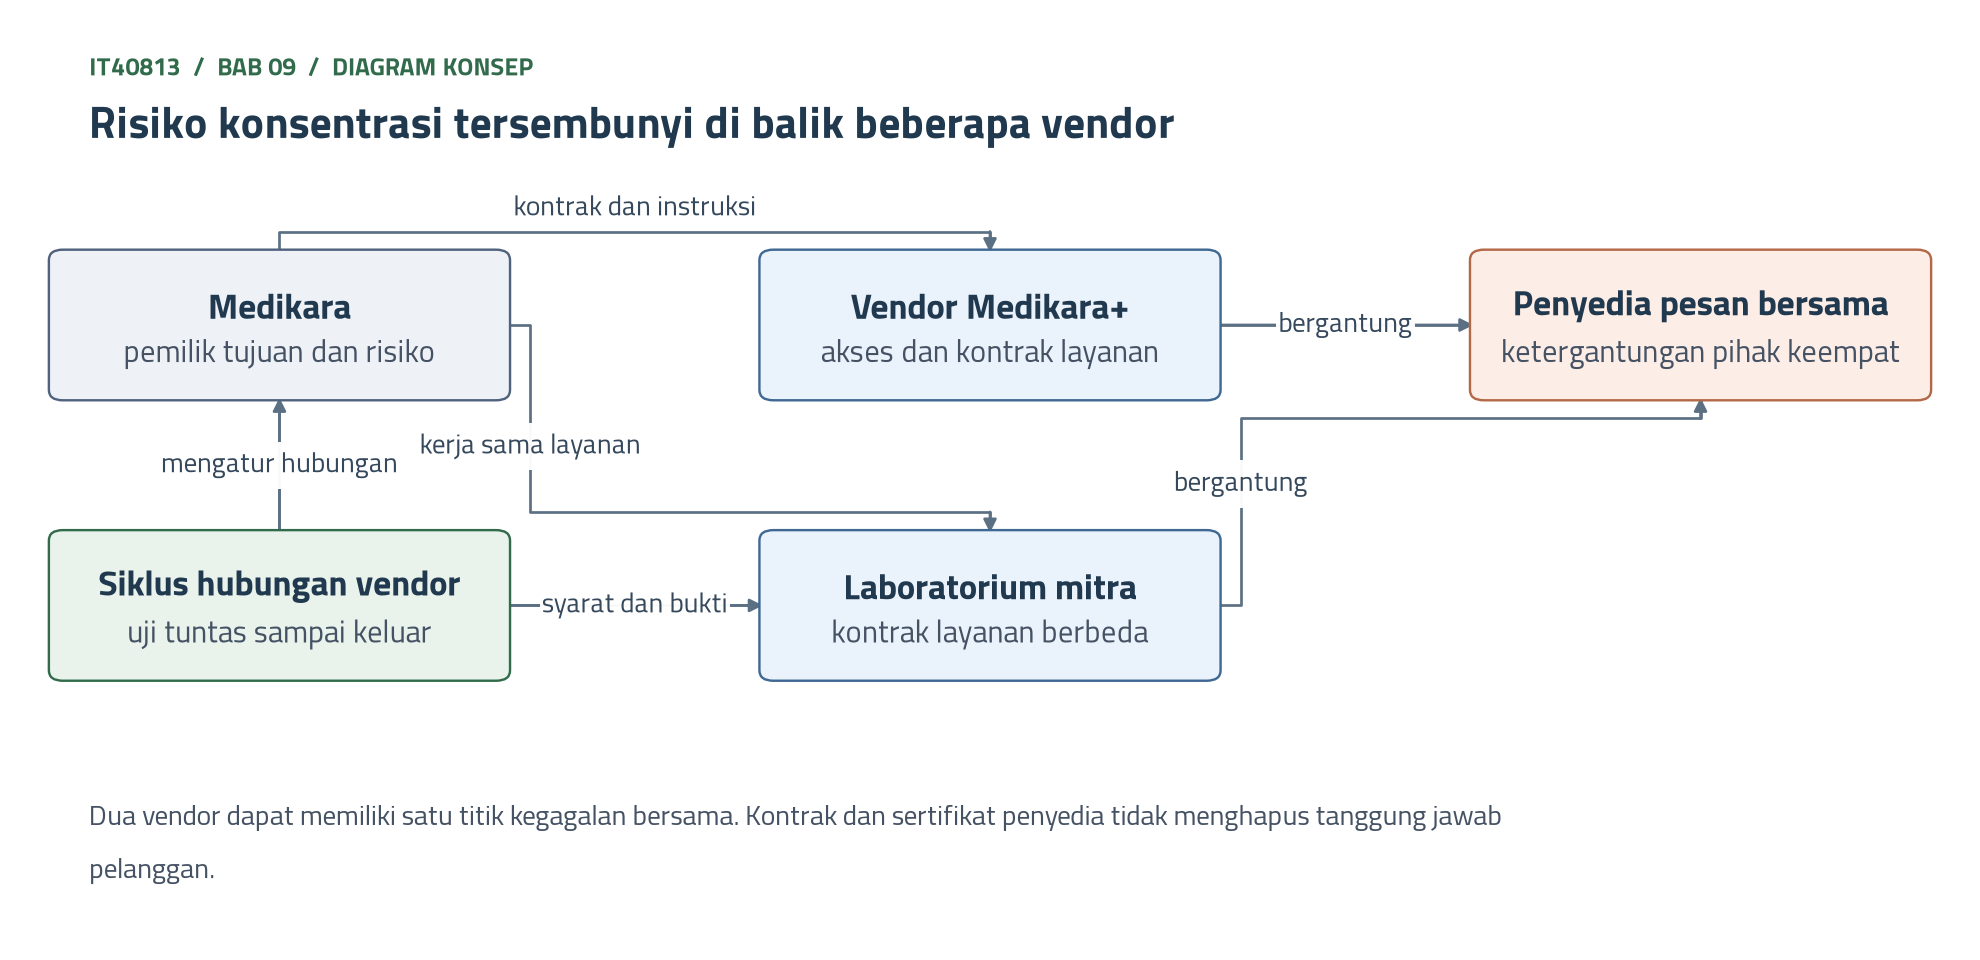
\includegraphics[width=\textwidth]{../figures/ch09-diagram-konsep.png}
  \caption{Risiko konsentrasi tersembunyi di balik beberapa vendor}
  \label{fig:ch09-ilustrasi-bab}
\end{figure}
}{}

\section{Rantai Pasok Digital dan Konsentrasi Risiko}

\subsection*{Pihak ketiga dan pihak keempat}

Pihak ketiga mencakup vendor aplikasi, penyedia cloud, mitra data, dan layanan pendukung. Pihak
keempat adalah pemasok yang dipakai pihak ketiga. NIST CSF 2.0 (Cybersecurity Framework) menyebut
teknologi bergantung pada ekosistem pasok yang saling terhubung, dengan beberapa lapis alih daya
\cite{nistcsf2}. Ketergantungan karena itu perlu ditelusuri melampaui nama vendor. Dua kontrak
berbeda dapat bergantung pada pusat data atau layanan identitas yang sama.

Analogi pemasok kantin menunjukkan konsentrasi. Dua pedagang yang membeli bahan dari gudang yang
sama tidak memberi keragaman pasokan ketika gudangnya tutup. Jumlah kontrak tidak sama dengan
jumlah sumber daya yang independen.

Dua contoh menuntut penelusuran lebih jauh:
\begin{enumerate}
  \item Misalkan vendor Medikara+ dan laboratorium mitra memakai penyedia pesan yang sama.
  Layanan pesan itu tersedia 99,5 persen dari 8.760 jam per tahun, sehingga gangguannya 43,8 jam
  per tahun. Bila kedua jalur benar-benar terpisah dan gangguannya tidak saling terkait, gangguan
  bersamaan hanya 0,5 persen dikali 0,5 persen, atau 0,0025 persen dari waktu. Angka itu setara
  sekitar 13 menit per tahun. Bila penyedianya sama, gangguan bersamaan menjadi 43,8 jam, atau
  200 kali lipat. Pengingat 336.000 janji temu per tahun ikut terganggu sekitar 0,5 persen, atau
  1.680 janji temu. Register Bab 5 mencatat skenario ini sebagai R-08 dengan skor
  $2 \times 4 = 8$.
  \item Misalkan cadangan ditempatkan di akun cloud yang sama dengan produksi. Akun yang diretas
  dapat membuat kedua salinan tidak dapat digunakan, meskipun medianya berbeda. Bab 3 mencatat
  144 uji pemulihan per tahun, yaitu 36 fasilitas dikali 4 uji. Seluruh uji itu dapat lulus tanpa
  menjawab skenario ini, bila setiap uji memakai akun pengelola yang sama. Bab 10 memakai temuan
  ini untuk R-05.
\end{enumerate}

Gambar~\ref{fig:ch09-peta} memperlihatkan peta ketergantungan pengandaian untuk lima hubungan
Medikara. Tabel~\ref{tab:ch09-rantai} merangkum pertanyaan yang perlu dijawab pada tiap hubungan.
Dari lima hubungan itu, penyedia pesan dan layanan identitas masing-masing dipakai dua hubungan.
V-01 menyentuh keduanya dan juga memakai V-02, sehingga vendor Medikara+ memiliki 3 penyedia
pendukung. Bab 7 memisalkan angka yang sama: Medikara perlu menunjukkan 3 persetujuan tertulis.

\begin{figure}[!htb]
  \centering
  \begin{tikzpicture}[
  font=\scriptsize,
  execute at begin node={\hyphenpenalty=10000},
  induk/.style={draw, rounded corners, align=center, text width=1.8cm,
    minimum height=1.3cm, fill=praditagreen!15},
  tahap/.style={draw, rounded corners, align=center, text width=3.1cm,
    minimum height=0.62cm, fill=blue!8},
  lanjut/.style={draw, rounded corners, align=center, text width=3.4cm,
    minimum height=0.62cm, fill=orange!12},
  masalah/.style={draw, rounded corners, align=center, text width=3.4cm,
    minimum height=0.9cm, fill=red!22},
  panah/.style={-{Stealth[length=2mm]}, thick}]
  \node[font=\scriptsize\bfseries] at (0,2.75) {Organisasi};
  \node[font=\scriptsize\bfseries] at (3.6,2.75) {Pihak ketiga};
  \node[font=\scriptsize\bfseries] at (8.1,2.75) {Pihak keempat};
  \node[induk] (m) at (0,0)
    {Medikara\\{\tiny\mdseries pemilik tujuan dan risiko}};
  \node[tahap] (v3) at (3.6,2) {V-03 Laboratorium mitra};
  \node[tahap] (v1) at (3.6,1) {V-01 Vendor Medikara+};
  \node[tahap] (v2) at (3.6,0) {V-02 Penyedia cloud};
  \node[tahap] (v4) at (3.6,-1) {V-04 Mitra asuransi};
  \node[tahap] (v5) at (3.6,-2) {V-05 Apotek daring};
  \node[masalah] (p1) at (8.1,1.6)
    {Penyedia pesan bersama\\{\tiny\mdseries titik kegagalan V-01 dan V-03}};
  \node[masalah] (p2) at (8.1,0.3)
    {Layanan identitas bersama\\{\tiny\mdseries titik kegagalan V-01 dan V-02}};
  \node[lanjut] (p3) at (8.1,-1) {Pengolah klaim};
  \node[lanjut] (p4) at (8.1,-2) {Kurir obat};
  \draw[panah] (m.east) -- (v3.west);
  \draw[panah] (m.east) -- (v1.west);
  \draw[panah] (m.east) -- (v2.west);
  \draw[panah] (m.east) -- (v4.west);
  \draw[panah] (m.east) -- (v5.west);
  \draw[panah] (v1.south) -- (v2.north);
  \draw[panah] (v3.east) -- (p1.west);
  \draw[panah] (v1.east) -- (p1.west);
  \draw[panah] (v1.east) -- (p2.west);
  \draw[panah] (v2.east) -- (p2.west);
  \draw[panah] (v4.east) -- (p3.west);
  \draw[panah] (v5.east) -- (p4.west);
\end{tikzpicture}

  \caption{Peta ketergantungan pihak ketiga dan pihak keempat (misalkan)}
  \label{fig:ch09-peta}
\end{figure}

\begin{table}[!htb]
  \centering\small
  \caption{Ketergantungan yang perlu ditelusuri (misalkan)}\label{tab:ch09-rantai}
  \begin{tabularx}{\textwidth}{|>{\raggedright\arraybackslash}X|>{\raggedright\arraybackslash}X|>{\raggedright\arraybackslash}X|}
    \hline
    \textbf{Hubungan} & \textbf{Pihak lanjutan} & \textbf{Pertanyaan} \\ \hline
    Vendor Medikara+ & Penyedia cloud, identitas, pesan, dan staf dukungan & Siapa dapat mengakses
    data, dan dari mana? \\ \hline
    Laboratorium mitra & Penyedia pesan bersama & Apakah ada titik kegagalan bersama? \\ \hline
    Cadangan data & Identitas dan akun pengelola & Apakah pemulihan tetap mungkin saat akun utama
    gagal? \\ \hline
    Mitra asuransi & Pengolah klaim & Siapa lagi menerima data klaim, dan untuk tujuan apa? \\
    \hline
    Apotek daring & Kurir obat & Data apa yang sampai ke kurir? \\ \hline
  \end{tabularx}
\end{table}

Dua hal sering tertukar: jumlah kontrak dan jumlah sumber daya yang independen. Pembagiannya
begini. Lima kontrak terlihat seperti lima pilihan. Bila dua di antaranya berhenti karena satu
penyedia yang sama, pilihannya tinggal tiga pada saat gangguan. Temuan ini punya dua konsekuensi.
Pertama, Medikara memerlukan inventaris layanan pemasok, yang pada NIST CSF tercantum sebagai
ID.AM-04 \cite{nistcsf2}. Kedua, kontrak harus mewajibkan vendor menyebut subprosesornya. Istilah
subprosesor pada bab ini sama dengan ``prosesor lain'' pada Pasal 51 ayat (5) UU PDP
\cite{uu27-2022-pdp}.

Diagram konsep pada awal bab meringkas pola itu. Medikara memegang tujuan dan risiko. Vendor
Medikara+ dan laboratorium mitra terikat kontrak layanan yang berbeda, tetapi keduanya bergantung
pada penyedia pesan bersama. Siklus hubungan vendor, dari uji tuntas sampai keluar, mengatur
hubungan itu lewat syarat dan bukti.

\subsection*{Membaca kejadian dan laporan industri}

Pertanyaan kemudian muncul: seberapa besar akibat pihak ketiga pada layanan kesehatan? Dua
kejadian dan satu laporan memberi pembacaan yang berbeda:
\begin{enumerate}
  \item Change Healthcare, Amerika Serikat. American Hospital Association (AHA) menyebut perusahaan
  ini memproses 15 miliar transaksi kesehatan per tahun, termasuk pemeriksaan kepesertaan,
  farmasi, klaim, dan pembayaran. Serangan terjadi pada 21 Februari 2024. Survei AHA pada 9 sampai
  12 Maret 2024 terhadap hampir 1.000 rumah sakit mencatat 94 persen mengalami dampak keuangan, 83
  persen dampak pada arus kas, dan 74 persen dampak pada pelayanan langsung pasien
  \cite{c09-aha-change}. Satu pihak ketiga yang berhenti dapat menyentuh banyak rumah sakit
  sekaligus.
  \item Synnovis, Inggris. NHS England London melaporkan serangan \textit{ransomware} pada 3 Juni
  2024 terhadap laboratorium patologi yang memproses tes darah bagi organisasi National Health
  Service (NHS), terutama di London bagian tenggara. Laporan mingguannya mencatat janji rawat jalan
  dan tindakan elektif yang ditunda pada dua \textit{trust} rumah sakit, dengan data manajemen yang
  belum diverifikasi \cite{c09-nhs-synnovis}. Angka rincinya tidak dikutip di sini, karena halaman
  laporan tidak dapat dibaca utuh saat pemeriksaan. Medikara memiliki laboratorium rujukan dan
  membuka kerja sama laboratorium mitra, sehingga polanya relevan.
\end{enumerate}

Laporan industri memberi gambaran lebih luas. Ringkasan WaterISAC atas Verizon Data Breach
Investigations Report (DBIR) 2026 menyebut keterlibatan pihak ketiga mencapai 48 persen
pelanggaran, naik 60 persen dari tahun sebelumnya \cite{c01-verizon-dbir2026,c09-waterisac-dbir}.
Data laporan industri dapat memberi konteks, tetapi persentase global tidak langsung menjadi
peluang insiden Medikara. Angka 48 persen adalah bagian dari seluruh pelanggaran yang dilaporkan,
bukan peluang satu rumah sakit mengalami insiden. Bab 5 tetap memakai peluang R-01 sebesar 0,2
per tahun, karena angka itu dinilai dari bukti Medikara.

Tabel~\ref{tab:ch09-pembacaan} merangkum cara membaca ketiga sumber. Tim memisahkan hasil survei,
definisi kejadian, dan bukti organisasi sebelum memakainya untuk keputusan risiko.

\begin{table}[!htb]
  \centering\small
  \caption{Membaca tiga sumber tentang risiko pihak ketiga}\label{tab:ch09-pembacaan}
  \begin{tabularx}{\textwidth}{|>{\raggedright\arraybackslash}p{0.2\textwidth}|>{\raggedright\arraybackslash}p{0.2\textwidth}|>{\raggedright\arraybackslash}X|>{\raggedright\arraybackslash}X|}
    \hline
    \textbf{Sumber} & \textbf{Jenis data} & \textbf{Yang berguna} & \textbf{Batas pembacaan} \\
    \hline
    Survei AHA & Laporan mandiri, beberapa pekan setelah serangan & Bentuk dampak pada kas dan
    pelayanan & Dibuat asosiasi rumah sakit; sistem pembiayaannya berbeda \\ \hline
    NHS England London & Data manajemen mingguan yang belum diverifikasi & Dampak dinyatakan dalam
    janji dan tindakan & Angka sementara; ukuran layanan berbeda \\ \hline
    DBIR 2026 lewat WaterISAC & Ringkasan laporan industri global & Tren keterlibatan pihak ketiga
    & Bagian dari pelanggaran, bukan peluang; definisi perlu dibaca pada laporan asli \\ \hline
  \end{tabularx}
\end{table}

\section{Siklus Hidup Risiko Pihak Ketiga}

\subsection*{Dari klasifikasi sampai keluar}

Manajemen pemasok dimulai sebelum pemilihan, dilanjutkan dengan kontrak, penerapan, pemantauan,
perubahan, dan penghentian. ISO/IEC 27036-2:2022 membahas persyaratan hubungan pengadaan dan
pemasok \cite{c09-iso27036}. NIST SP 800-161 Rev. 1 membahas identifikasi, penilaian, dan
pengurangan risiko rantai pasok siber pada semua tingkat organisasi \cite{c09-nist-sp800161}.
NIST CSF 2.0 merumuskan hasil yang dituju pada kategori GV.SC, dan menyebut SP 800-161 sebagai
bacaan mendalam \cite{nistcsf2}. Bab 8 menargetkan objektif COBIT APO10 \textit{Managed vendors}
pada tingkat 3 \cite{cobit2019-intro}.

Analogi menyewa kendaraan memperjelas siklusnya. Penyewa memeriksa kondisi sebelum menerima,
mencatat aturan penggunaan, memantau gangguan, lalu memeriksa keadaan saat mengembalikan. Tanda
tangan awal tidak menyelesaikan seluruh tanggung jawab.

Gambar~\ref{fig:ch09-siklus} memperlihatkan siklus kendali pihak ketiga dari klasifikasi sampai
keluar. Tabel~\ref{tab:ch09-siklus} memasangkan tiap tahap dengan hasil NIST CSF dan bukti pada
Medikara. Rumusan hasil pada tabel adalah ringkasan bab. Dari enam baris itu, hanya GV.SC-07 yang
masuk profil target Bab 8. Lima baris lain dipakai sebagai pertanyaan kerja, tanpa mengubah profil
16 dari 106 subkategori.

\begin{figure}[!htb]
  \centering
  \begin{tikzpicture}[
  font=\scriptsize,
  execute at begin node={\hyphenpenalty=10000},
  tahap/.style={draw, rounded corners, align=center, text width=1.85cm,
    minimum height=1.2cm, fill=blue!8},
  catatan/.style={align=center, font=\tiny\mdseries},
  panah/.style={-{Stealth[length=2mm]}, thick}]
  \node[tahap] (n0) at (0,0) {Klasifikasi\\{\tiny\mdseries GV.SC-04}};
  \node[tahap] (n1) at (2.5,0) {Uji tuntas\\{\tiny\mdseries GV.SC-06}};
  \node[tahap, fill=orange!12] (n2) at (5,0) {Kontrak\\{\tiny\mdseries GV.SC-05}};
  \node[tahap] (n3) at (7.5,0) {Penerapan dan pemantauan\\{\tiny\mdseries GV.SC-07}};
  \node[tahap, fill=green!10] (n4) at (10,0) {Keluar dan verifikasi\\{\tiny\mdseries GV.SC-10}};
  \node[tahap, fill=red!22] (ins) at (7.5,-2) {Insiden bersama\\{\tiny\mdseries GV.SC-08}};
  \draw[panah] (n0) -- (n1);
  \draw[panah] (n1) -- (n2);
  \draw[panah] (n2) -- (n3);
  \draw[panah] (n3) -- (n4);
  \draw[panah] (n3) -- (ins);
  \draw[panah, rounded corners] (ins.west) -| (n2.south);
  \draw[panah, rounded corners] (n3.north) -- ++(0,0.45) -| (n0.north);
  \node[catatan] at (3.75,1.32)
    {perubahan tujuan, subprosesor, lokasi, atau skala memicu klasifikasi ulang};
  \node[catatan, anchor=east] at (6.3,-2.2) {temuan memperbaiki klausul};
\end{tikzpicture}

  \caption{Siklus kendali pihak ketiga dari klasifikasi sampai keluar}
  \label{fig:ch09-siklus}
\end{figure}

\begin{table}[!htb]
  \centering\small
  \caption{Tahap siklus, hasil NIST CSF, dan bukti Medikara (misalkan)}\label{tab:ch09-siklus}
  \begin{tabularx}{\textwidth}{|>{\raggedright\arraybackslash}p{0.19\textwidth}|>{\raggedright\arraybackslash}p{0.14\textwidth}|>{\raggedright\arraybackslash}X|>{\raggedright\arraybackslash}X|}
    \hline
    \textbf{Tahap} & \textbf{Hasil} & \textbf{Ringkasan hasil} & \textbf{Bukti pada Medikara} \\
    \hline
    Klasifikasi & GV.SC-04 & Pemasok dikenal dan diprioritaskan menurut kekritisan & Register
    pemasok dengan skor \\ \hline
    Uji tuntas & GV.SC-06 & Perencanaan dan uji tuntas sebelum hubungan resmi & Kuesioner beserta
    bukti dan cakupan \\ \hline
    Kontrak & GV.SC-05 & Persyaratan masuk kontrak dan perjanjian & 11 dari 11 butir; klausul K-05
    \\ \hline
    Penerapan dan pemantauan & GV.SC-07 & Risiko dinilai dan dipantau sepanjang hubungan & 60 dari
    60 catatan AC-01; tinjauan triwulanan \\ \hline
    Insiden bersama & GV.SC-08 & Pemasok dilibatkan dalam rencana insiden dan pemulihan & 2 latihan
    per tahun; laporan 12 jam \\ \hline
    Keluar & GV.SC-10 & Rencana mencakup kegiatan setelah hubungan berakhir & Hasil uji ekspor dan
    bukti penghapusan \\ \hline
  \end{tabularx}
\end{table}

\subsection*{Klasifikasi: seberapa dalam pemeriksaannya?}

Klasifikasi menentukan kedalaman pemeriksaan. Tiga pertanyaan cukup untuk memulai: data apa yang
disentuh, layanan apa yang berhenti bila pihak itu gagal, dan seberapa sulit menggantinya.
Pemeriksaan yang sama untuk semua pemasok memboroskan tenaga pada pemasok kecil dan mengurangi
perhatian pada pemasok kritis.

Analogi tamu rumah sakit membantu. Pengantar bunga cukup mendaftar di lobi. Teknisi yang masuk
ruang obat perlu surat tugas, pendamping, dan catatan keluar. Keduanya tamu, tetapi risikonya
berbeda.

Dua contoh menentukan tingkat pemeriksaan:
\begin{enumerate}
  \item Misalkan penyedia cetak materi umum tidak menerima data pribadi dan mudah diganti. Skornya
  1 dari 9, sehingga pemeriksaan dasar memadai. Vendor Medikara+ mengolah data kesehatan untuk
  28.000 janji temu per bulan dan mendukung layanan lintas fasilitas. Skornya 9 dari 9. Uji akses,
  insiden, pemulihan, subprosesor, serta strategi keluar menjadi prioritas.
  \item Misalkan register pemasok memuat 40 hubungan: 5 tingkat terperinci, 12 menengah, dan 23
  dasar. Pemeriksaan memakan 40, 16, dan 4 jam per hubungan. Totalnya 200 tambah 192 tambah 92,
  atau 484 jam, yaitu Rp29,04 juta pada tarif Rp60.000 per jam dari Bab 7. Bila seluruh 40
  hubungan diperiksa terperinci, diperlukan 1.600 jam atau Rp96 juta. Pembagian tingkat menghemat
  1.116 jam, sekitar 70 persen, dan pemeriksaan terperinci tetap jatuh pada hubungan penting.
\end{enumerate}

Tabel~\ref{tab:ch09-klasifikasi} menerapkan skala pengandaian pada enam hubungan. Kolom Data,
Kritis, dan Ganti menilai akses data, kekritisan layanan, dan kesulitan mengganti, masing-masing
0 sampai 3. Skor 7 sampai 9 berarti terperinci, 4 sampai 6 menengah, dan 0 sampai 3 dasar.
Salinannya tersedia di \berkas{sources/chapter09/klasifikasi-vendor.csv}. Skala ini rancangan
pembelajaran, bukan rumus standar.

\begin{table}[!htb]
  \centering\small
  \caption{Klasifikasi enam hubungan Medikara (misalkan)}\label{tab:ch09-klasifikasi}
  \begin{tabularx}{\textwidth}{|>{\raggedright\arraybackslash}p{0.07\textwidth}|>{\raggedright\arraybackslash}X|*{4}{>{\centering\arraybackslash}p{0.08\textwidth}|}>{\raggedright\arraybackslash}p{0.15\textwidth}|}
    \hline
    \textbf{ID} & \textbf{Hubungan} & \textbf{Data} & \textbf{Kritis} & \textbf{Ganti} &
    \textbf{Skor} & \textbf{Tingkat} \\ \hline
    V-01 & Vendor Medikara+ & 3 & 3 & 3 & 9 & Terperinci \\ \hline
    V-02 & Penyedia cloud & 3 & 3 & 2 & 8 & Terperinci \\ \hline
    V-03 & Laboratorium mitra & 3 & 3 & 2 & 8 & Terperinci \\ \hline
    V-04 & Mitra asuransi & 3 & 2 & 2 & 7 & Terperinci \\ \hline
    V-05 & Apotek daring & 2 & 2 & 1 & 5 & Menengah \\ \hline
    V-06 & Penyedia cetak materi & 0 & 0 & 1 & 1 & Dasar \\ \hline
  \end{tabularx}
\end{table}

Klasifikasi tidak sekadar menghasilkan warna. Vendor kritis harus memiliki pemilik hubungan,
jadwal tinjau, indikator, pemicu eskalasi, dan rencana bila gagal. Misalkan 5 hubungan terperinci
ditinjau tiap triwulan selama 8 jam. Bebannya 5 dikali 4 dikali 8, atau 160 jam per tahun, atau
Rp9,6 juta. Perubahan subprosesor, lokasi, atau tujuan data memicu pemeriksaan ulang sebelum
persetujuan perubahan.

\subsection*{Uji tuntas: dari jawaban ke bukti}

Uji tuntas meminta bukti, bukan janji. Tim menanyakan siapa mengakses data, di mana data berada,
siapa subprosesornya, dan kapan pemulihan terakhir diuji. Tiap jawaban lalu dinilai dari jenis
buktinya. Daftar sepuluh pertanyaan tersedia di
\berkas{sources/chapter09/kuesioner-uji-tuntas.md}.

Analogi membeli rumah bekas menjelaskan bedanya. Penjual berkata atapnya tidak bocor. Pembeli
melihat langit-langit saat hujan dan meminta catatan perbaikan. Jawaban penjual tetap berguna,
tetapi hanya sebagai titik awal pemeriksaan.

Dua contoh menunjukkan batas jawaban:
\begin{enumerate}
  \item Misalkan vendor menjawab ya pada 10 dari 10 pertanyaan. Saat bukti diminta, 7 jawaban
  memiliki bukti dalam cakupan layanan, 2 memiliki bukti di luar cakupan, dan 1 tanpa bukti. Yang
  dapat diandalkan 7 dari 10, atau 70 persen, bukan 100 persen. Tiga baris sisanya menjadi syarat
  kontrak atau risiko sisa yang diputuskan.
  \item Skor keamanan eksternal disusun dari informasi publik, tanpa masuk ke sistem pemasok.
  Keskin dan rekan membandingkan metode semacam itu dan menyimpulkan skornya memiliki kemiripan,
  tetapi tidak sepenuhnya menyatu untuk organisasi yang sama \cite{c09-keskin2021}. Misalkan dua
  layanan memberi vendor yang sama nilai 85 dan 62 dari 100. Selisih 23 poin itu bukan keputusan.
  Tim memakainya untuk memilih pertanyaan lanjutan.
\end{enumerate}

Tabel~\ref{tab:ch09-bukti} menyusun empat jenis bukti, dari yang paling lemah sampai yang paling
kuat. Urutan ini penafsiran bab. Bukti yang kuat juga lebih mahal, sehingga uji bersama dipilih
untuk hubungan terperinci.

\begin{table}[!htb]
  \centering\small
  \caption{Empat jenis bukti uji tuntas (penafsiran bab)}\label{tab:ch09-bukti}
  \begin{tabularx}{\textwidth}{|>{\raggedright\arraybackslash}p{0.23\textwidth}|>{\raggedright\arraybackslash}X|>{\raggedright\arraybackslash}X|}
    \hline
    \textbf{Jenis} & \textbf{Contoh} & \textbf{Yang perlu diperiksa} \\ \hline
    1. Jawaban vendor & Kuesioner, CAIQ & Tanggal dan siapa yang menjawab \\ \hline
    2. Dokumen vendor & Kebijakan, prosedur & Apakah dijalankan pada layanan yang dibeli \\ \hline
    3. Laporan independen & Sertifikat, laporan SOC 2 & Cakupan, periode, dan pengecualian \\ \hline
    4. Uji bersama & Uji ekspor, latihan insiden, uji pemulihan & Hasil, kekurangan, dan uji ulang
    \\ \hline
  \end{tabularx}
\end{table}

\subsection*{Pemantauan dan perubahan}

Kontrak yang baik dapat melemah selama masa berlakunya. GV.SC-07 meminta risiko pemasok dipantau
sepanjang hubungan \cite{nistcsf2}. Pemantauan memakai indikator yang punya ambang, pemilik, dan
tindakan. Laporan tahunan vendor saja tidak memenuhi kebutuhan itu.

Analogi katering kantor menunjukkan alasannya. Dapur yang baik pada Januari belum tentu baik pada
Juni. Pengurus kantor mencicipi contoh, mencatat keterlambatan, dan menanyakan pergantian pemasok
bahan.

Dua contoh memperlihatkan pemantauan yang berguna:
\begin{enumerate}
  \item Bab 6 memisalkan pencabutan AC-01 turun dari 24 akun menjadi 9, 5, dan 2 akun. Penurunan
  itu hanya berarti bila seluruh 120 akun tercakup, karena sebelumnya 12 akun luput. Peninjauan
  bulanan pada 5 rumah sakit menghasilkan 60 catatan per tahun. Bab 8 menetapkan 60 dari 60 catatan
  dan 120 dari 120 akun cocok sebagai bukti penerimaan.
  \item Misalkan kontrak meminta pemberitahuan 30 hari sebelum subprosesor berganti. Alur tinjauan
  paralel Bab 8 memakan 10 hari kerja, sekitar 14 hari kalender. Sisa 16 hari dipakai untuk menguji
  layanan pengganti. Bila vendor hanya memberi tahu 7 hari sebelumnya, tinjauan tidak selesai, dan
  keputusan menjadi menerima risiko atau menunda perubahan.
\end{enumerate}

Tabel~\ref{tab:ch09-pantau} merangkum indikator awal untuk hubungan terperinci. Bab 13 mengolahnya
menjadi indikator risiko dengan batas dari Bab 5.

\begin{table}[!htb]
  \centering\small
  \caption{Indikator pemantauan hubungan terperinci (misalkan)}\label{tab:ch09-pantau}
  \begin{tabularx}{\textwidth}{|>{\raggedright\arraybackslash}X|>{\raggedright\arraybackslash}p{0.2\textwidth}|>{\raggedright\arraybackslash}X|>{\raggedright\arraybackslash}p{0.19\textwidth}|}
    \hline
    \textbf{Indikator} & \textbf{Ambang} & \textbf{Tindakan bila terlewati} & \textbf{Pemilik} \\
    \hline
    Akun vendor tanpa pemilik & 0 akun (Bab 5) & Bekukan akun dan catat penyimpangan & Pemilik
    Medikara+ \\ \hline
    Catatan peninjauan AC-01 & 60 dari 60 per tahun & Eskalasi ke kepala TI & Pemilik layanan \\
    \hline
    Laporan dugaan insiden & 12 jam (K-05) & Catat pelanggaran kontrak dan tagih perbaikan &
    Pengelola vendor \\ \hline
    Latihan insiden bersama & 2 per tahun & Masuk temuan Paket C & Petugas pelindungan data \\
    \hline
    Pemberitahuan subprosesor & 30 hari sebelumnya & Tunda perubahan atau putuskan risiko sisa &
    Pemilik layanan \\ \hline
    Uji ekspor & 1 per tahun & Tinjau ulang skor R-10 & Pengelola vendor \\ \hline
  \end{tabularx}
\end{table}

\subsection*{Strategi keluar}

Strategi keluar menjawab cara mengakhiri hubungan tanpa menghentikan layanan dan tanpa meninggalkan
data. GV.SC-10 meminta rencana mencakup kegiatan setelah hubungan berakhir \cite{nistcsf2}. Rencana
itu mencakup ekspor, pemindahan, pencabutan akses, dan penghapusan yang terverifikasi. Kata
``keluar'' juga berlaku bagi vendor yang gagal mendadak.

Analogi pindah kontrakan membantu. Penyewa yang baik tahu barang apa yang miliknya, berapa lama
mengangkutnya, dan siapa memegang kunci terakhir. Kontrak sewa yang menyebut ``boleh pindah kapan
saja'' tidak menjawab ketiga hal itu.

Dua contoh menunjukkan mengapa keluar perlu diuji:
\begin{enumerate}
  \item Misalkan vendor menjanjikan ekspor data, tetapi hanya menyediakan gambar dokumen tanpa
  metadata. Tim menguji format, kelengkapan, waktu, dan biaya ekspor sebelum menerima layanan. Pada
  uji dengan 10.000 rekam sintetis, 9.600 rekam terbaca mesin, atau 96 persen. Sisa 4 persen dari
  336.000 rekam janji temu per tahun adalah 13.440 rekam. Dengan 5 menit per rekam, pekerjaan
  manualnya 1.120 jam, atau Rp67,2 juta.
  \item Bab 5 memisalkan R-10 berpeluang 0,1 per tahun dengan kerugian Rp800 juta, yang berasal
  dari migrasi darurat 3 bulan pada 84.000 janji temu. Harapan kerugiannya Rp80 juta per tahun.
  Tabel~\ref{tab:ch09-keluar} membandingkan dua opsi pada latihan bab itu.
\end{enumerate}

\begin{table}[!htb]
  \centering\small
  \caption{Dua opsi penanganan R-10 (misalkan, mengikuti Bab 5)}\label{tab:ch09-keluar}
  \begin{tabularx}{\textwidth}{|>{\raggedright\arraybackslash}X|>{\raggedright\arraybackslash}p{0.11\textwidth}|>{\raggedright\arraybackslash}p{0.19\textwidth}|>{\raggedright\arraybackslash}p{0.09\textwidth}|>{\raggedright\arraybackslash}p{0.09\textwidth}|>{\raggedright\arraybackslash}p{0.11\textwidth}|}
    \hline
    \textbf{Opsi} & \textbf{Biaya sekali} & \textbf{Harapan setelahnya} & \textbf{Turun per tahun} &
    \textbf{Balik modal} & \textbf{Pemutus} \\ \hline
    Uji ekspor dan pendampingan & Rp60 juta & 0,1 kali Rp300 juta, atau Rp30 juta & Rp50 juta & 1,2
    tahun & Kepala TI \\ \hline
    Ganti vendor segera & Rp300 juta & 0,05 kali Rp800 juta, atau Rp40 juta & Rp40 juta & 7,5 tahun
    & Komite \\ \hline
  \end{tabularx}
\end{table}

Perbandingan ini punya dua konsekuensi. Pertama, mengganti vendor bukan otomatis pilihan yang
paling aman. Vendor baru dapat memakai subpenyedia yang sama, sehingga R-08 tidak berubah. Kedua,
uji ekspor memberi manfaat lebih cepat, tetapi tidak menghapus keahlian yang hanya dimiliki vendor.
Risiko sisanya tetap dicatat.

\begin{kasus}[title={Kasus Medikara Health: Lima Hubungan, Dua Prioritas}]
Tim mengisi register pemasok dan mendapat empat hubungan terperinci dari lima hubungan target.
Aktivitas bab ini meminta dua hubungan paling kritis. V-01 jelas terpilih dengan skor 9. V-02 dan
V-03 sama-sama 8. Tim memakai satu pemutus tambahan, yaitu jumlah layanan yang berhenti. V-02
menampung seluruh platform target, sehingga V-02 dipilih.

Keputusan ini punya dua konsekuensi. Pertama, V-03 tetap diperiksa terperinci, tetapi klausul
lengkapnya disusun pada gelombang berikutnya, dan risikonya tetap tercatat pada R-08. Kedua, biaya
perlu diakui terus terang. Bab 8 menganggarkan Rp120 juta per tahun untuk APO10 tingkat 3. Harapan
kerugian R-10 turun Rp50 juta per tahun bila uji ekspor dilakukan. Selisihnya dibenarkan oleh K-05
yang berstatus tidak memenuhi dan oleh hak pasien, bukan oleh hitungan rupiah semata. Pemilik
layanan memegang akuntabilitas atas subprosesor dan penghentian vendor, sesuai baris 10 RACI Bab 8.
\end{kasus}

\section{Klausul Kontrak dan Kewajiban Prosesor}

\subsection*{Dari janji menjadi ukuran}

Kontrak menerjemahkan kebutuhan kendali menjadi kewajiban yang dapat ditagih. Unsur penting meliputi
instruksi pemrosesan, pembatasan tujuan, akses, subprosesor, bukti kontrol, insiden, pemulihan, dan
pengembalian atau penghapusan data. Ketentuan prosesor harus diperiksa terhadap UU PDP, bukan hanya
janji kerahasiaan umum. Pasal 51 mewajibkan prosesor bekerja berdasarkan perintah pengendali. Pasal
52 memberlakukan sejumlah kewajiban pengendali kepada prosesor \cite{uu27-2022-pdp}. Bab 7 sudah
membaca pasal-pasal itu, dan bab ini mengubahnya menjadi klausul.

Analogi jasa pengiriman membantu membedakan janji dan bukti. Pernyataan barang dijaga belum
menjelaskan siapa menerima, kapan keterlambatan diberitahukan, dan bagaimana kehilangan ditangani.
Kontrak membutuhkan ukuran serta jalur pelaksanaan.

Dua contoh menunjukkan akibat klausul yang kabur:
\begin{enumerate}
  \item Misalkan kontrak hanya meminta pemberitahuan insiden secepatnya. Medikara tidak dapat
  menagih apa pun karena tidak ada batasnya. Register Bab 3 menetapkan batas kontraktual 12 jam
  sejak vendor mendeteksi dugaan insiden (K-05), beserta pembaruan berkala. Angka ini pilihan
  kontrak, bukan tenggat undang-undang. Bila vendor mendeteksi pada Jumat 20.00, batasnya Sabtu
  08.00.
  \item Misalkan kontrak berbunyi vendor menjaga kerahasiaan data. Kalimat itu tidak berkata apa
  pun tentang akun yang tetap aktif setelah pekerjaan selesai, padahal itulah sebab insiden 2025.
  Klausul pengganti menuntut tiap akun punya pemilik dan tanggal berakhir, dan akun dicabut paling
  lambat 1 hari kerja setelah penugasan selesai. Buktinya 120 dari 120 akun cocok dengan daftar
  penugasan.
\end{enumerate}

Gambar~\ref{fig:ch09-waktu} menempatkan klausul 12 jam pada garis waktu Bab 7. Laporan tepat waktu
menyisakan 48 jam sampai batas internal jam ke-60 dan 60 jam sampai batas terluar. Varian Bab 3,
yaitu laporan setelah 30 jam, melanggar kontrak 18 jam dan menyisakan 30 jam serta 42 jam. Hitungan
ini mengandaikan kegagalan dan penemuan bersamaan, seperti asumsi Bab 3 dan Bab 7. Pasal 46 ayat (1)
tidak memakai frasa sejak diketahui secara eksplisit, sehingga fungsi hukum menetapkan titik
mulainya.

\begin{figure}[!htb]
  \centering
  \begin{tikzpicture}[
  font=\scriptsize,
  execute at begin node={\hyphenpenalty=10000},
  atas/.style={align=center, text width=1.6cm, inner sep=0pt, anchor=south},
  bawah/.style={align=center, text width=1.6cm, inner sep=0pt, anchor=north,
    font=\tiny\mdseries},
  rentang/.style={{Stealth[length=1.6mm]}-{Stealth[length=1.6mm]}, thick},
  nilai/.style={fill=white, inner sep=1pt, font=\tiny\bfseries}]
  \fill[green!10] (0,0) rectangle (1.68,0.28);
  \fill[red!22] (1.68,0) rectangle (4.2,0.28);
  \fill[blue!8] (4.2,0) rectangle (8.4,0.28);
  \fill[orange!12] (8.4,0) rectangle (10.08,0.28);
  \draw (0,0) rectangle (10.08,0.28);
  \foreach \x in {0,1.68,4.2,8.4,10.08} {
    \draw[thick] (\x,-0.08) -- (\x,0.36);
  }
  \node[atas] at (0,0.42) {Jam 0\\{\tiny\mdseries Jumat 20.00}};
  \node[atas] at (1.68,0.42) {Jam 12\\{\tiny\mdseries Sabtu 08.00}};
  \node[atas] at (4.2,0.42) {Jam 30\\{\tiny\mdseries Minggu 02.00}};
  \node[atas] at (8.4,0.42) {Jam 60\\{\tiny\mdseries Senin 08.00}};
  \node[atas] at (10.08,0.42) {Jam 72\\{\tiny\mdseries Senin 20.00}};
  \node[bawah] at (0,-0.14) {Vendor mendeteksi};
  \node[bawah] at (1.68,-0.14) {Batas K-05};
  \node[bawah] at (4.2,-0.14) {Varian Bab 3: terlambat 18 jam};
  \node[bawah] at (8.4,-0.14) {Batas internal naskah};
  \node[bawah] at (10.08,-0.14) {Batas terluar Pasal 46};
  \draw[rentang] (1.68,-1.02) -- node[nilai] {48 jam} (8.4,-1.02);
  \draw[rentang] (1.68,-1.42) -- node[nilai] {60 jam} (10.08,-1.42);
  \draw[rentang] (4.2,-1.82) -- node[nilai] {30 jam} (8.4,-1.82);
  \draw[rentang] (4.2,-2.22) -- node[nilai] {42 jam} (10.08,-2.22);
  \node[align=right, anchor=east, font=\tiny\mdseries] at (1.6,-1.22)
    {laporan pada\\jam ke-12};
  \node[align=right, anchor=east, font=\tiny\mdseries] at (4.12,-2.02)
    {laporan pada\\jam ke-30};
\end{tikzpicture}

  \caption{Klausul laporan 12 jam pada garis waktu pemberitahuan (misalkan)}
  \label{fig:ch09-waktu}
\end{figure}

Dua hal pada kontrak sering tertukar: ganti rugi dan tanggung jawab. Pembagiannya begini. Ganti
rugi dapat memindahkan biaya. Biaya langsung insiden pada hitungan IT40613 adalah Rp14,4 juta untuk
penanganan dan Rp9,3 juta untuk pemberitahuan kepada 620 pasien, atau Rp23,7 juta. Vendor dapat
diminta mengganti angka itu. Kewajiban memberi tahu menurut Pasal 46 tetap berada pada Medikara
sebagai pengendali \cite{uu27-2022-pdp}. Kepercayaan pasien juga tidak berpindah lewat kontrak.

Tabel~\ref{tab:ch09-kontrak} merangkum sembilan pokok klausul beserta ukuran penerimaan dan bukti.
Lembar kerjanya ada di \berkas{sources/chapter09/klausul-kontrak.md}. Ukuran internalnya mengikuti
dokumen Bab 8: KB-02 untuk akun vendor, KB-03 untuk pencabutan, dan KB-07 untuk pemberitahuan
insiden. Isinya rancangan pembelajaran, bukan naskah siap tanda tangan.

\begin{table}[!htb]
  \centering\small
  \caption{Klausul contoh dan bukti penerimaan (misalkan)}\label{tab:ch09-kontrak}
  \begin{tabularx}{\textwidth}{|>{\raggedright\arraybackslash}p{0.25\textwidth}|>{\raggedright\arraybackslash}X|>{\raggedright\arraybackslash}X|}
    \hline
    \textbf{Pokok} & \textbf{Ukuran penerimaan} & \textbf{Bukti} \\ \hline
    Instruksi dan batas tujuan & Tujuan tertulis; perubahan lewat persetujuan & Daftar instruksi
    berversi \\ \hline
    Pengguna dan peninjauan akses & Pemilik dan tanggal berakhir; cabut dalam 1 hari kerja & 120
    dari 120 akun cocok; AC-01 \\ \hline
    Subprosesor & Persetujuan tertulis; pemberitahuan 30 hari & Daftar penerima dan persetujuan \\
    \hline
    Lokasi dan akses dukungan & Di dalam wilayah Indonesia, kecuali izin sesuai Pasal 972 &
    Inventaris lokasi data, cadangan, dan akses \\ \hline
    Laporan dugaan insiden & Laporan awal 12 jam; 2 latihan per tahun & Kronologi dan hasil latihan
    \\ \hline
    Catatan aktivitas & Per orang; disimpan 90 hari & Uji telusur satu rekam \\ \hline
    Pemeriksaan dan asurans & Bukti dapat ditinjau sesuai cakupan & Laporan, pengecualian, dan
    tindak lanjut \\ \hline
    Ekspor dan biaya keluar & Format dan tenggat disepakati; ekspor lengkap & Hasil uji ekspor
    tahunan \\ \hline
    Penghapusan dan cadangan & Terverifikasi, termasuk salinan cadangan & Berita acara penghapusan
    \\ \hline
  \end{tabularx}
\end{table}

\subsection*{Enam dari sebelas butir}

Pertanyaan berikutnya: butir apa yang perlu ditawar ulang? Salinan pihak ketiga PP 33/2026 Pasal 14
memuat 11 butir minimum perjanjian, antara lain cakupan, jenis data, jangka waktu, serta mekanisme
pengawasan dan audit \cite{c03-pp33-nonresmi,c07-rsm-pp33}. Peraturan itu baru berlaku 16 Januari
2027 dan naskah resminya belum diperoleh, sehingga bab ini memakainya sebagai daftar periksa, bukan
kewajiban.

Bab 7 memisalkan perjanjian vendor Medikara+ hanya memuat 6 dari 11 butir, dan Bab 8 menargetkan 11
dari 11. Rincian kelima butir kosong belum dapat dicocokkan ke naskah resmi. Tim karena itu
memetakannya ke lima pokok kontrol berikut, dan pemetaan ini penafsiran bab:
\begin{enumerate}
  \item instruksi pemrosesan yang tertulis,
  \item daftar akun dan subprosesor,
  \item pencabutan akses saat penugasan selesai,
  \item mekanisme pengawasan dan audit,
  \item pengembalian dan penghapusan data saat kontrak berakhir.
\end{enumerate}

Tiga pokok pertama menjawab CP-01 pada Bab 7. Laporan 12 jam tidak masuk daftar ini, karena
klausulnya sudah ada pada K-05. Masalah K-05 adalah pelaksanaan, sehingga jawabannya latihan
bersama, bukan kalimat baru. Waktu pulih kontrak juga berada di luar kelima pokok ini. Bab 10
memisalkan kontrak V-01 menjanjikan pemulihan 24 jam dan layanan identitas 8 jam, lalu membawa
selisihnya terhadap RTO ke tawar ulang tersendiri. Bila naskah resmi tersedia, tim mencocokkan ulang
kelima pokok itu.

\subsection*{Peran menentukan klausul}

Tidak semua hubungan memakai kontrak yang sama. Tabel~\ref{tab:ch09-peran} memperlihatkan peran awal
tiap hubungan. Bab 7 sudah menempatkan vendor sebagai prosesor untuk janji temu dan mitra asuransi
sebagai pengendali terpisah, dan keduanya penafsiran yang perlu ditinjau fungsi hukum. Panduan
European Data Protection Board menyebut peran ditentukan kegiatan nyata, bukan sebutan dalam kontrak
\cite{c07-edpb-roles}. Panduan itu tidak mengikat di Indonesia.

\begin{table}[!htb]
  \centering\small
  \caption{Peran awal tiap hubungan dan akibatnya pada kontrak (penafsiran bab)}
  \label{tab:ch09-peran}
  \begin{tabularx}{\textwidth}{|>{\raggedright\arraybackslash}p{0.21\textwidth}|>{\raggedright\arraybackslash}p{0.23\textwidth}|>{\raggedright\arraybackslash}X|}
    \hline
    \textbf{Hubungan} & \textbf{Peran awal} & \textbf{Akibat pada kontrak} \\ \hline
    Vendor Medikara+ & Prosesor & Perintah tertulis; persetujuan subprosesor; Pasal 51 dan Pasal 52
    \\ \hline
    Penyedia cloud & Prosesor atau subprosesor & Syarat Pasal 966 ayat (5) PP 28/2024; data
    dikendalikan penuh Medikara \\ \hline
    Laboratorium mitra & Perlu analisis per kegiatan & Hasil kepada dokter berbeda dari layanan
    laboratorium untuk tujuan sendiri \\ \hline
    Mitra asuransi & Pengendali terpisah & Tujuan, dasar, dan data minimum; DPIA sebelum aktif \\
    \hline
    Program kesehatan karyawan & Pengendali bersama bila tujuan ditentukan bersama & Syarat Pasal
    18; perusahaan hanya menerima hasil agregat \\ \hline
  \end{tabularx}
\end{table}

Perjanjian dengan mitra sektor keuangan dapat membawa persyaratan tambahan melalui kontrak. Tim
memeriksa pihak yang langsung diatur, dasar ketentuan, dan bagian yang mengalir kepada Medikara.
Aturan untuk lembaga jasa keuangan tidak otomatis berlaku langsung kepada semua penyedia layanan
kesehatan. Bab 3 mencatat dua baris yang berbeda: K-15 tidak berlaku karena Medikara bukan lembaga
jasa keuangan nonbank, sedangkan K-12 mengikat lewat kontrak. K-12 meminta Medikara melapor gangguan
kepada mitra asuransi dalam 1 jam, dan contoh Bab 3 mencatat hanya 2 dari 12 gangguan tepat waktu.
Kewajiban kontrak karena itu berjalan dua arah. Medikara menagih vendor, dan mitra menagih Medikara.

\begin{kasus}[title={Kasus Medikara Health: Tiga Klausul yang Menjawab Insiden 2025}]
Tim menguji klausul terhadap kronologi Bab 7. Akun dukungan tetap aktif setelah kontrak pekerjaan
selesai, panggilan berlangsung 8 malam, dan catatan rinci hanya disimpan 7 hari. Catatan itu juga
hanya memuat ID aplikasi, bukan ID orang.

Klausul pertama mencabut akun paling lambat 1 hari kerja setelah penugasan selesai. Bila
dijalankan, akun itu tidak aktif pada malam pertama, sehingga peristiwanya tidak terjadi. Klausul
kedua mewajibkan pemantauan akses dan laporan dugaan insiden dalam 12 jam. Bila akses di luar
penugasan terdeteksi pada malam pertama, rekam yang terbaca paling banyak 155, bukan 1.240, atau
turun 87,5 persen. Bila deteksi terjadi setelah dua malam, jumlahnya 310, atau turun 75 persen.
Klausul ketiga mewajibkan catatan per orang yang disimpan 90 hari. Pada kronologi itu, 620 rekam
malam 1 sampai 4 tinggal jumlah karena catatannya terhapus. Dengan masa simpan 90 hari, seluruh 8
malam masih dapat ditelusuri pada hari ke-11.

Keputusan ini punya dua konsekuensi. Pertama, ketiga klausul membutuhkan pekerjaan di sisi
Medikara. Daftar penugasan harus tersedia, dan AC-01 tetap dijalankan, karena Pasal 37 dan Pasal 39
UU PDP tetap menuntut pengawasan oleh pengendali \cite{uu27-2022-pdp}. Kedua, klausul tidak menjawab
bahwa Medikara mengetahui kejadian lewat keluhan pasien. Hal itu memerlukan tinjauan catatan
aktivitas di sisi Medikara, yang masuk Paket D pada Bab 8.
\end{kasus}

\section{Cloud dan Tanggung Jawab Bersama}

\subsection*{Tiga model layanan}

NIST SP 800-145 mendefinisikan cloud sebagai model akses jaringan ke kumpulan sumber daya komputasi
yang dapat disediakan dan dilepas dengan cepat. Definisi itu menyebut lima karakteristik, tiga model
layanan, dan empat model penyebaran \cite{c09-nist-sp800145}. Ketiga model layanan adalah
\textit{Infrastructure as a Service} (IaaS), \textit{Platform as a Service} (PaaS), dan
\textit{Software as a Service} (SaaS). Model tanggung jawab bersama, atau \textit{shared
responsibility model}, membagi pekerjaan penyedia dan pelanggan pada tiap model. Amazon Web Services
(AWS) merumuskan tanggung jawabnya sebagai \textit{security of the cloud}. Tanggung jawab pelanggan
disebut \textit{security in the cloud}, dan besarnya ditentukan layanan yang dipilih
\cite{c09-aws-shared}.

Analogi sewa tempat usaha menjelaskan batasnya. Pengelola gedung menjaga struktur bangunan, tetapi
penyewa tetap mengatur kunci ruang, pegawai, dan dokumennya. Membayar sewa tidak otomatis menjaga
seluruh kegiatan di dalam ruangan.

Dua contoh membantah asumsi pemindahan penuh:
\begin{enumerate}
  \item Misalkan Medikara memakai IaaS untuk 40 server virtual. Penyedia mengelola fasilitas dan
  virtualisasi, sementara tim Medikara masih mengelola sistem operasi serta aplikasi. Bila pembaruan
  memakan 1 jam per server per bulan, bebannya 40 jam per bulan, atau 480 jam per tahun, atau Rp28,8
  juta. Tim platform 6 orang memiliki 960 jam kerja per bulan, sehingga pembaruan saja memakan
  sekitar 4,2 persen kapasitasnya.
  \item Misalkan Medikara memakai SaaS. Penyedia mengoperasikan aplikasi, tetapi pelanggan tetap
  mengatur pengguna, hak akses, tujuan penggunaan, dan prosedur keluar. Peninjauan 120 akun tetap
  milik Medikara, yaitu 12 peninjauan pada 5 rumah sakit, atau 60 catatan per tahun. Penyedia hanya
  menyediakan fungsinya.
\end{enumerate}

Gambar~\ref{fig:ch09-cloud} memperlihatkan pembagian umum menurut panduan Microsoft
\cite{c09-ms-shared}. Panduan itu menyatakan pembagiannya ilustratif dan tidak mengubah perjanjian
layanan, sehingga pembagian harus dikonfirmasi pada kontrak. Pelanggan memegang penuh 7 dari 10
lapisan pada IaaS, 4 dari 10 pada PaaS, dan 3 dari 10 pada SaaS. Dua lapisan lain pada PaaS dan SaaS
dibagi bersama. Pada SaaS sekalipun, 5 dari 10 lapisan masih memerlukan kerja pelanggan.

\begin{figure}[!htb]
  \centering
  \begin{tikzpicture}[
  font=\scriptsize,
  lapisan/.style={draw, align=left, text width=3.5cm, minimum height=0.42cm, inner xsep=3pt,
    inner ysep=0pt, fill=praditagreen!15},
  judul/.style={draw, align=center, minimum width=2.3cm, minimum height=0.42cm,
    inner ysep=0pt, fill=praditagreen!15, font=\scriptsize\bfseries},
  pel/.style={draw, align=center, minimum width=2.3cm, minimum height=0.42cm, inner ysep=0pt,
    fill=orange!12},
  ber/.style={draw, align=center, minimum width=2.3cm, minimum height=0.42cm, inner ysep=0pt,
    fill=blue!8},
  pen/.style={draw, align=center, minimum width=2.3cm, minimum height=0.42cm, inner ysep=0pt,
    fill=green!10}]
  \node[lapisan, font=\scriptsize\bfseries] at (0,0) {Lapisan};
  \node[judul] at (3.2,0) {IaaS};
  \node[judul] at (5.5,0) {PaaS};
  \node[judul] at (7.8,0) {SaaS};
  \node[lapisan] at (0,-0.42) {Data pelanggan};
  \node[pel] at (3.2,-0.42) {Pelanggan};
  \node[pel] at (5.5,-0.42) {Pelanggan};
  \node[pel] at (7.8,-0.42) {Pelanggan};
  \node[lapisan] at (0,-0.84) {Konfigurasi dan pengaturan};
  \node[pel] at (3.2,-0.84) {Pelanggan};
  \node[pel] at (5.5,-0.84) {Pelanggan};
  \node[pel] at (7.8,-0.84) {Pelanggan};
  \node[lapisan] at (0,-1.26) {Identitas dan pengguna};
  \node[pel] at (3.2,-1.26) {Pelanggan};
  \node[pel] at (5.5,-1.26) {Pelanggan};
  \node[pel] at (7.8,-1.26) {Pelanggan};
  \node[lapisan] at (0,-1.68) {Perangkat klien};
  \node[pel] at (3.2,-1.68) {Pelanggan};
  \node[pel] at (5.5,-1.68) {Pelanggan};
  \node[ber] at (7.8,-1.68) {Bersama};
  \node[lapisan] at (0,-2.1) {Aplikasi};
  \node[pel] at (3.2,-2.1) {Pelanggan};
  \node[ber] at (5.5,-2.1) {Bersama};
  \node[ber] at (7.8,-2.1) {Bersama};
  \node[lapisan] at (0,-2.52) {Kendali jaringan};
  \node[pel] at (3.2,-2.52) {Pelanggan};
  \node[ber] at (5.5,-2.52) {Bersama};
  \node[pen] at (7.8,-2.52) {Penyedia};
  \node[lapisan] at (0,-2.94) {Sistem operasi};
  \node[pel] at (3.2,-2.94) {Pelanggan};
  \node[pen] at (5.5,-2.94) {Penyedia};
  \node[pen] at (7.8,-2.94) {Penyedia};
  \node[lapisan] at (0,-3.36) {Host fisik};
  \node[pen] at (3.2,-3.36) {Penyedia};
  \node[pen] at (5.5,-3.36) {Penyedia};
  \node[pen] at (7.8,-3.36) {Penyedia};
  \node[lapisan] at (0,-3.78) {Jaringan fisik};
  \node[pen] at (3.2,-3.78) {Penyedia};
  \node[pen] at (5.5,-3.78) {Penyedia};
  \node[pen] at (7.8,-3.78) {Penyedia};
  \node[lapisan] at (0,-4.2) {Pusat data fisik};
  \node[pen] at (3.2,-4.2) {Penyedia};
  \node[pen] at (5.5,-4.2) {Penyedia};
  \node[pen] at (7.8,-4.2) {Penyedia};
\end{tikzpicture}

  \caption{Pembagian lapisan menurut panduan Microsoft; kontrak layanan tetap menentukan}
  \label{fig:ch09-cloud}
\end{figure}

Dua hal sering tertukar: tanggung jawab kerja dan tanggung jawab hukum. Pembagiannya begini. Matriks
tanggung jawab menjawab siapa mengatur, menjalankan, dan memantau tiap kendali. Pasal 51 ayat (3) UU
PDP menjawab hal lain: pemrosesan oleh prosesor termasuk tanggung jawab pengendali
\cite{uu27-2022-pdp}. Penyedia dapat mengerjakan seluruh lapisan fisik, tetapi Medikara tetap
pengendali data pasien.

Tabel~\ref{tab:ch09-matriks} menerapkan pembagian itu sebagai matriks kendali. Salinannya ada di
\berkas{sources/chapter09/matriks-cloud.csv}. Tim mengisi model layanan berdasarkan rancangan
IT40713, bukan asumsi dari nama model saja. Banyak solusi memakai campuran model layanan
\cite{c09-ms-shared}.

\begin{table}[!htb]
  \centering\small
  \caption{Matriks kendali cloud yang harus dikonfirmasi kontrak (misalkan)}\label{tab:ch09-matriks}
  \begin{tabularx}{\textwidth}{|>{\raggedright\arraybackslash}p{0.2\textwidth}|>{\raggedright\arraybackslash}X|>{\raggedright\arraybackslash}X|>{\raggedright\arraybackslash}p{0.21\textwidth}|}
    \hline
    \textbf{Kendali} & \textbf{Penyedia} & \textbf{Medikara} & \textbf{Bukti} \\ \hline
    Fasilitas fisik & Operasikan dan lindungi & Tinjau asurans dan cakupan & Ruang lingkup laporan
    \\ \hline
    Sistem operasi pada IaaS & Konfirmasi batas layanan & Konfigurasi dan pembaruan & Hasil
    pembaruan \\ \hline
    Hak pengguna pada SaaS & Sediakan fungsi akses & Setujui dan tinjau lewat AC-01 & Daftar hak dan
    pencabutan \\ \hline
    Tujuan dan klasifikasi data & Dukung kewajiban layanan & Tetapkan tujuan dan dasar & Catatan
    pemrosesan \\ \hline
    Pemulihan & Penuhi bagian kontrak & Uji hasil layanan & Hasil uji terpadu \\ \hline
    Keluar dan penghapusan & Ekspor serta hapus sesuai peran & Verifikasi kelengkapan & Hasil uji
    keluar \\ \hline
  \end{tabularx}
\end{table}

\subsection*{Sertifikat, laporan SOC 2, dan CCM}

Asurans adalah keyakinan dari pihak lain atas kendali penyedia. Bentuknya beragam, dan tiap bentuk
menjawab pertanyaan berbeda. Sertifikat ISO/IEC 27001 menilai sistem manajemen dalam ruang lingkup
tertentu \cite{iso27001-2022}. Annex A memuat kontrol A.5.23 tentang keamanan pemakaian layanan
cloud \cite{c06-dqs-annexa}. ISO/IEC 27036-4:2016 memberi panduan bagi pelanggan dan penyedia untuk
memahami serta mengelola risiko layanan cloud, tetapi tidak mencakup kelangsungan bisnis
\cite{c09-iso27036-4}. Laporan System and Organization Controls (SOC) membantu pengguna menilai
risiko alih daya \cite{c09-aicpa-soc}.

Analogi sertifikat laik sehat restoran menjelaskan batasnya. Sertifikat menilai dapur pada waktu dan
cakupan tertentu. Sertifikat itu tidak menjawab apakah pesanan sampai ke meja yang benar. Bagian itu
diatur pelanggan dan pelayan pada hari itu.

Dua contoh menunjukkan cara membaca bukti:
\begin{enumerate}
  \item Bab 6 memisalkan vendor Medikara+ memiliki sertifikat yang masih berlaku 14 bulan, tetapi
  ruang lingkupnya hanya pengembangan aplikasi. Akun dukungan yang masuk ke data pasien tidak
  termasuk. Masa berlaku yang panjang tidak menutup celah cakupan itu.
  \item Misalkan laporan SOC 2 Type 2 penyedia mencakup 1 Januari sampai 30 Juni 2026, dan tim
  membacanya pada 1 November 2026. Empat bulan terakhir belum tercakup. Bagian pengujian mencatat 3
  pengecualian dari 25 sampel pencabutan akses, atau 12 persen. Laporan juga memuat 14 kontrol
  pelengkap pengguna (\textit{complementary user entity controls}), dan Medikara baru menjalankan 9.
  Lima sisanya adalah pekerjaan Medikara, bukan pekerjaan penyedia.
\end{enumerate}

Tabel~\ref{tab:ch09-asurans} merangkum empat bentuk bukti. SOC 2 memeriksa kendali pada kategori
keamanan, ketersediaan, integritas pemrosesan, kerahasiaan, atau privasi. Type 1 menilai rancangan
dan penerapan kendali pada satu tanggal. Type 2 menambahkan pengujian efektivitas operasi selama
periode tertentu, umumnya 6 sampai 12 bulan \cite{c09-deloitte-soc}. CCM versi 4.1 memuat 197
objektif kontrol dalam 17 domain, dan CAIQ mengubahnya menjadi pertanyaan ya atau tidak
\cite{c09-ccm}. Catat versi unduhan, karena jawaban kuesioner tetap merupakan klaim yang perlu
dibuktikan. Bab 12 membahas laporan asurans lebih rinci.

\begin{table}[!htb]
  \centering\small
  \caption{Empat bentuk bukti penyedia dan cara membacanya}\label{tab:ch09-asurans}
  \begin{tabularx}{\textwidth}{|>{\raggedright\arraybackslash}p{0.2\textwidth}|>{\raggedright\arraybackslash}X|>{\raggedright\arraybackslash}X|}
    \hline
    \textbf{Bentuk} & \textbf{Yang dijawab} & \textbf{Yang harus dibaca} \\ \hline
    CAIQ & Apa yang dinyatakan penyedia & Versi, tanggal, layanan, dan bukti tiap jawaban ya \\
    \hline
    Sertifikat ISO/IEC 27001 & Apakah sistem manajemen memenuhi persyaratan pada ruang lingkup itu
    & Ruang lingkup, lokasi, masa berlaku, dan penerbit \\ \hline
    SOC 2 Type 1 & Apakah kendali dirancang dan diterapkan pada satu tanggal & Tanggal, kategori,
    dan uraian sistem \\ \hline
    SOC 2 Type 2 & Apakah kendali bekerja selama satu periode & Periode, pengecualian, kontrol
    pelengkap pengguna dan subpenyedia \\ \hline
  \end{tabularx}
\end{table}

\subsection*{Lokasi data dan akses dukungan}

Pertanyaan kemudian muncul: bolehkah data pasien berada pada layanan cloud di luar negeri? Bab 3 dan
Bab 7 sudah membaca aturannya. Pasal 21 PP 71/2019 mengizinkan Penyelenggara Sistem Elektronik (PSE)
lingkup privat mengelola sistem dan data di dalam atau di luar wilayah Indonesia
\cite{pp71-2019-pste}. Ketentuan umum ini tidak otomatis berlaku bagi rekam medis, karena aturan
kesehatan lebih khusus. Pasal 966 ayat (2) PP 28/2024 menyatakan pangkalan data kesehatan berupa
pusat data di dalam wilayah Indonesia. Ayat (5) mengizinkan jasa pihak lain bila dilaksanakan di
dalam wilayah Indonesia, berdasarkan perjanjian kerja sama, dengan data yang dimiliki dan
dikendalikan penuh oleh penyelenggara. Pasal 972 mengatur transfer ke luar wilayah hukum untuk
tujuan spesifik dan terbatas, dengan izin Menteri, serta memenuhi syarat transfer data pribadi
\cite{pp28-2024-kesehatan}. Hubungan aturan umum dan aturan khusus pada kasus nyata tetap perlu
dinilai penasihat hukum.

Analogi gudang arsip menjelaskan mengapa lokasi saja belum cukup. Gudang boleh berada di kota yang
benar, tetapi kuncinya dapat dipegang petugas di kota lain. Pemilik arsip menanyakan letak gudang
dan juga siapa yang dapat membuka pintunya.

Dua contoh berangka:
\begin{enumerate}
  \item Bab 3 memisalkan vendor menawarkan penyimpanan di luar negeri seharga Rp420 juta per tahun,
  dibanding Rp600 juta saat ini. Penghematannya Rp180 juta, atau 30 persen. Nilai kontrak melewati
  batas Rp400 juta, sehingga keputusan naik ke direksi. Usulan berhenti pada Pasal 966 ayat (2),
  karena harga tidak menjawab lokasi pusat data. Pilihan yang tersisa adalah menawar ulang dengan
  fasilitas dalam negeri, atau memisahkan data bukan rekam medis setelah dinilai.
  \item Bab 7 memisalkan 4 staf dukungan vendor di luar negeri membuka layar Medikara+ untuk sekitar
  300 tiket per bulan. Pasal 971 ayat (2) PP 28/2024 menyebut penampilan sebagai salah satu bentuk
  transfer \cite{pp28-2024-kesehatan}, sehingga akses itu diperlakukan sebagai transfer, dan ini
  penafsiran Bab 7. Dukungan dalam negeri lebih mahal Rp25 juta per bulan, atau Rp300 juta per
  tahun, atau sekitar Rp83.000 per tiket. Selisih itu dibandingkan dengan beban izin Pasal 972 atau
  pemakaian data sintetis.
\end{enumerate}

Tabel~\ref{tab:ch09-lokasi} menyusun pertanyaan yang diajukan kepada penyedia cloud. Baris register
terkait adalah K-07 dan K-13, dan celah terkait adalah CP-07. Bab 3 memperlakukan salinan cadangan
sebagai bagian dari penyimpanan, dan perlakuan itu penafsiran bab, karena Pasal 966 tidak menyebut
cadangan secara tersendiri.

\begin{table}[!htb]
  \centering\small
  \caption{Pertanyaan lokasi dan akses kepada penyedia cloud (penafsiran bab)}
  \label{tab:ch09-lokasi}
  \begin{tabularx}{\textwidth}{|>{\raggedright\arraybackslash}p{0.17\textwidth}|>{\raggedright\arraybackslash}X|>{\raggedright\arraybackslash}p{0.24\textwidth}|>{\raggedright\arraybackslash}X|}
    \hline
    \textbf{Aspek} & \textbf{Pertanyaan} & \textbf{Dasar penelusuran} & \textbf{Bukti} \\ \hline
    Pusat data & Di mana data aktif disimpan? & PP 28/2024 Pasal 966 ayat (2) & Inventaris lokasi \\
    \hline
    Cadangan & Di mana salinan cadangan berada? & Pasal 966; Permenkes 24/2022 Pasal 20 & Prosedur
    dan hasil uji \\ \hline
    Jasa pihak lain & Apakah data tetap dikendalikan penuh? & Pasal 966 ayat (5); Permenkes Pasal 22
    & Perjanjian dan rekomendasi \\ \hline
    Akses dukungan & Dari negara mana staf dapat melihat data? & Pasal 971 ayat (2) dan Pasal 972 &
    Daftar staf dan catatan akses \\ \hline
    Transfer & Apakah ada tujuan spesifik dan izin? & Pasal 972; UU PDP Pasal 56 & Izin Menteri dan
    penilaian \\ \hline
  \end{tabularx}
\end{table}

\section{Berbagi Data dan Penilaian Dampak}

\subsection*{Pemicu dan tujuan DPIA}

DPIA menilai dampak pemrosesan terhadap subjek data. Pasal 34 ayat (1) UU PDP mewajibkannya bila
pemrosesan berpotensi risiko tinggi. Ayat (2) menyebut tujuh keadaan, antara lain data spesifik,
skala besar, serta pencocokan atau penggabungan data \cite{uu27-2022-pdp}. Bab 7 membaca satu
keadaan sudah cukup, dan pembacaan itu penafsiran bab. Tim menjelaskan tujuan, kebutuhan,
proporsionalitas, alur, risiko, kontrol, risiko sisa, dan keputusan sebelum alur berisiko
diaktifkan.

Analogi membuka akses jalan di kawasan perumahan menunjukkan tujuan penilaian. Jalan baru
mempercepat perjalanan, tetapi mengubah lalu lintas dan keselamatan penghuni. Penilaian tidak hanya
menghitung pendapatan pengelola, karena akibat pada warga juga perlu dipertimbangkan.

Dua contoh menunjukkan mengapa nama mitra belum cukup:
\begin{enumerate}
  \item Misalkan mitra asuransi meminta seluruh riwayat medis 10.000 pasien untuk verifikasi
  kepesertaan. Tim menguji apakah status kepesertaan dan data minimum sudah memenuhi tujuan.
  Pengiriman riwayat lengkap tidak diterima hanya karena mitra memiliki sistem yang aman. Bab 7
  menghitung alur klaim 6.000 per bulan, atau 72.000 per tahun. Bagi 10.000 pasien itu, rata-ratanya
  7,2 klaim per pasien per tahun.
  \item Misalkan hasil laboratorium dikirim kepada dokter yang merawat. Tim membatasi penerima,
  tujuan, data, dan waktu akses. Kebutuhan layanan tidak menghapus risiko salah penerima. Misalkan 1
  dari 2.000 pengiriman salah alamat pada uji coba. Bila ada 300 pengiriman per hari, kesalahannya
  sekitar 55 per tahun, sehingga uji negatif dilakukan sebelum produksi.
\end{enumerate}

Gambar~\ref{fig:ch09-dpia} memperlihatkan alurnya. Urutan ini mengikuti alur 10 hari kerja pada Bab
8 dan kebijakan KB-05 tentang berbagi data dengan mitra. Petugas pelindungan data memimpin DPIA,
direktur pelayanan memutuskan tujuan, dan risiko sisa di atas batas naik ke direksi. Kepala rekam
medis memegang hak henti sempit bila dasar pemrosesan belum ada.

\begin{figure}[!htb]
  \centering
  \begin{tikzpicture}[
  font=\scriptsize,
  execute at begin node={\hyphenpenalty=10000},
  tahap/.style={draw, rounded corners, align=center, text width=2.35cm,
    minimum height=1.05cm, fill=blue!8},
  panah/.style={-{Stealth[length=2mm]}, thick}]
  \node[tahap] (n1) at (0,0)
    {Pemicu Pasal 34\\{\tiny\mdseries tujuh keadaan ayat (2)}};
  \node[tahap] (n2) at (3,0)
    {Tujuan dan kebutuhan\\{\tiny\mdseries data apa yang perlu}};
  \node[tahap] (n3) at (6,0)
    {Peta data\\{\tiny\mdseries sumber, penerima, lokasi}};
  \node[tahap] (n4) at (9,0)
    {Dampak pada pasien\\{\tiny\mdseries bukan hanya rupiah}};
  \node[tahap] (n5) at (9,-1.75)
    {Kontrol dan risiko sisa\\{\tiny\mdseries bukti uji sebelum aktif}};
  \node[tahap, fill=orange!12] (n6) at (6,-1.75)
    {Keputusan tujuan\\{\tiny\mdseries direktur pelayanan}};
  \node[tahap, fill=green!10] (n7) at (3,-1.75)
    {Aktif dengan syarat\\{\tiny\mdseries pemilik layanan}};
  \node[tahap] (n8) at (0,-1.75)
    {Pantau dan tinjau ulang\\{\tiny\mdseries bila tujuan atau skala berubah}};
  \node[tahap, fill=red!22] (n9) at (6,-3.5)
    {Hentikan atau naik\\{\tiny\mdseries risiko sisa di atas batas ke direksi}};
  \draw[panah] (n1) -- (n2);
  \draw[panah] (n2) -- (n3);
  \draw[panah] (n3) -- (n4);
  \draw[panah] (n4) -- (n5);
  \draw[panah] (n5) -- (n6);
  \draw[panah] (n6) -- (n7);
  \draw[panah] (n7) -- (n8);
  \draw[panah] (n6) -- node[right, align=left, font=\tiny\mdseries]
    {kurangi data,\\nilai ulang} (n3);
  \draw[panah] (n6) -- (n9);
\end{tikzpicture}

  \caption{Alur DPIA untuk berbagi data dengan mitra (penafsiran bab)}
  \label{fig:ch09-dpia}
\end{figure}

\subsection*{Mengurangi data lebih dahulu}

Dua hal sering tertukar: kontrol keamanan dan kebutuhan data. Pembagiannya begini. Enkripsi
melindungi data dalam perjalanan, tetapi penerima yang sah tetap dapat memakai seluruh isinya.
Pertanyaan pertama karena itu adalah data apa yang perlu dikirim. Kontrol baru dipasang pada data
yang lolos pertanyaan itu.

Tabel~\ref{tab:ch09-minimasi} menghitung akibatnya. Misalkan riwayat lengkap memuat rata-rata 30
rekam per pasien dan 42 kolom per rekam. Data minimum untuk klaim memerlukan 9 kolom. Hitungan
memakai jumlah nilai data sebagai ukuran paparan, bukan ukuran risiko. Riwayat lengkap menghasilkan
12,6 juta nilai data, sedangkan data minimum 648.000, atau turun sekitar 94,9 persen. Dibanding
klaim lengkap, data minimum tetap turun sekitar 78,6 persen.

\begin{table}[!htb]
  \centering\small
  \caption{Tiga pilihan data alur asuransi (misalkan)}\label{tab:ch09-minimasi}
  \begin{tabularx}{\textwidth}{|>{\raggedright\arraybackslash}X|>{\raggedright\arraybackslash}p{0.27\textwidth}|>{\centering\arraybackslash}p{0.11\textwidth}|>{\raggedright\arraybackslash}p{0.17\textwidth}|}
    \hline
    \textbf{Pilihan} & \textbf{Rekam} & \textbf{Kolom} & \textbf{Nilai data} \\ \hline
    Riwayat lengkap & $10.000 \times 30 = 300.000$ & 42 & 12.600.000 \\ \hline
    Klaim lengkap & 72.000 per tahun & 42 & 3.024.000 \\ \hline
    Data minimum & 72.000 per tahun & 9 & 648.000 \\ \hline
  \end{tabularx}
\end{table}

Tabel~\ref{tab:ch09-dpia} merangkum penilaian dampak alur ini. Kolom risiko membicarakan pasien,
bukan Medikara. Templatnya ada di \berkas{sources/chapter09/templat-dpia.md}, dan contoh terisinya
ada di \berkas{sources/chapter09/contoh-dpia-medikara.md}.

\begin{table}[!htb]
  \centering\small
  \caption{Contoh penilaian dampak alur asuransi (misalkan)}\label{tab:ch09-dpia}
  \begin{tabularx}{\textwidth}{|>{\raggedright\arraybackslash}X|>{\raggedright\arraybackslash}X|>{\raggedright\arraybackslash}X|}
    \hline
    \textbf{Risiko terhadap pasien} & \textbf{Pengurangan yang diusulkan} & \textbf{Risiko sisa dan
    keputusan} \\ \hline
    Riwayat berlebih memengaruhi perlakuan & Kirim status dan 9 kolom minimum sesuai tujuan & Nilai
    kemungkinan penggabungan ulang \\ \hline
    Salah penerima & Verifikasi mitra dan pembatasan akses & Uji negatif sebelum produksi \\ \hline
    Penggunaan tujuan lain & Instruksi, kontrak, dan pemantauan & Hentikan alur bila penggunaan
    menyimpang \\ \hline
  \end{tabularx}
\end{table}

\begin{kasus}[title={Kasus Medikara Health: DPIA Alur Asuransi}]
CP-03 pada Bab 7 mencatat DPIA alur asuransi belum ada, dan Bab 8 menjadikannya syarat alur berbagi
data. Alur klaim menyentuh tiga keadaan Pasal 34 ayat (2): data spesifik, skala besar, dan
penggabungan data. DPIA dikerjakan 3 orang selama 3 hari kerja, atau 72 jam, atau Rp4,32 juta.
Pekerjaan itu mengisi hari ke-2 sampai ke-4 pada alur 10 hari kerja.

Misalkan mitra tetap meminta riwayat lengkap. Tim menolak permintaan itu dan mengusulkan data
minimum 9 kolom. Mitra meminta waktu 1 bulan untuk mengubah sistemnya. Selama itu klaim diproses
manual: 6.000 klaim kali 5 menit, atau 500 jam, atau Rp30 juta. Petugas pelindungan data memberi
saran tertulis, dan direktur pelayanan memutuskan menunggu.

Keputusan ini punya dua konsekuensi. Pertama, Rp30 juta adalah biaya yang diterima secara sadar demi
mengurangi paparan pasien sekitar 94,9 persen. Keputusan itu tercatat bersama alasannya. Kedua, DPIA
tidak selesai saat alur aktif. Perubahan tujuan, kolom, penerima, lokasi, atau skala memicu
penilaian ulang. Bila mitra kemudian memakai data klaim untuk menilai premi perorangan, alur
dihentikan sampai tujuan baru dinilai. Peran dan kebutuhan datanya perlu ditinjau fungsi hukum.
\end{kasus}

\begin{pendalaman}
Software Bill of Materials (SBOM) membantu mengidentifikasi komponen perangkat lunak. Daftar
komponen bukan bukti bebas kerentanan. Misalkan SBOM vendor memuat 180 komponen, dan 6 di antaranya
memiliki kerentanan yang diketahui. Tim bertanya komponen mana yang benar-benar dipakai pada jalur
data pasien, dan kapan perbaikannya.

Saat membaca uji penetrasi vendor, periksa tanggal, cakupan, pembatasan, temuan, perbaikan, dan uji
ulang. Pengujian langsung hanya dilakukan pada sistem sendiri atau dengan izin tertulis. Tim teknis
juga dapat menilai kontrol vendor dengan CCM seri 4, lalu mencatat versi berkas yang dipakai
\cite{c09-ccm}. Strategi migrasi cloud dibahas pada IT40713, dan keamanan teknis Application
Programming Interface (API) dibahas pada IT40613.
\end{pendalaman}

\section{Aktivitas: Kerangka Pihak Ketiga, Matriks Cloud, dan DPIA}

\textbf{Tujuan.} Tim menyusun kerangka pihak ketiga untuk rancangan target, mengisi matriks tanggung
jawab bersama, dan menyusun DPIA satu alur berbagi data. Tim memakai organisasi nyata dengan izin
dan data yang dianonimkan, atau kasus Medikara Health.

\textbf{Pembagian peran.} Anggota berlatar bisnis menilai kekritisan vendor. Analis regulasi
memimpin penyusunan klausul kontrak dan DPIA. Analis teknologi mengisi matriks cloud. Analis risiko
menghubungkan hasil dengan R-01, R-08, dan R-10.

\textbf{Langkah kerja.}
\begin{enumerate}
  \item Isi \berkas{sources/chapter09/klasifikasi-vendor.csv} untuk penyedia cloud, vendor
  Medikara+, laboratorium mitra, asuransi, dan apotek daring. Hitung skor, lalu tetapkan tingkat
  pemeriksaan.
  \item Isi \berkas{sources/chapter09/peta-ketergantungan.csv}. Tandai pihak keempat yang dipakai
  lebih dari satu hubungan.
  \item Pilih dua hubungan paling kritis. Gunakan \berkas{sources/chapter09/kuesioner-uji-tuntas.md}
  dan \berkas{sources/chapter09/klausul-kontrak.md}.
  \item Tentukan indikator pemantauan, perubahan yang memicu tinjau ulang, serta strategi keluar dan
  uji ekspor.
  \item Isi \berkas{sources/chapter09/matriks-cloud.csv} berdasarkan layanan yang dirancang IT40713,
  bukan asumsi nama model saja.
  \item Isi \berkas{sources/chapter09/templat-dpia.md} untuk satu alur asuransi. Bandingkan dengan
  \berkas{sources/chapter09/contoh-dpia-medikara.md}.
  \item Simulasikan dugaan insiden vendor pada Jumat 20.00. Pastikan kontrak dan matriks menunjukkan
  siapa menyelidiki, menghentikan alur, dan memberi informasi sebelum Sabtu 08.00.
\end{enumerate}

\textbf{Luaran.} Kerangka pihak ketiga, matriks tanggung jawab cloud, DPIA satu alur, dan catatan
simulasi.

\textbf{Kaitan dengan capstone.} Luaran masuk tonggak C3 Kondisi Target. Matriks diselaraskan dengan
layanan IT40713, dan alur data mitra diselaraskan dengan rancangan platform IT40613. Bab 10 memakai
hubungan kritis dan strategi keluar, sedangkan Bab 12 menguji klausul sebagai bukti audit.

\textbf{Kriteria penilaian.} Klasifikasi dan bukti 25 persen; kontrak serta pemantauan 25 persen;
kejelasan tanggung jawab 25 persen; analisis dampak dan risiko sisa 25 persen. Dokumen contoh bukan
nasihat kontrak untuk ditandatangani. Penilaian berfokus pada penalaran dan keterlacakan.

\textbf{Berkas pendukung.} Seluruh lembar kerja ada di \berkas{sources/chapter09/}, dengan daftar
berkas pada \berkas{sources/chapter09/README.md}. Data pasien, rahasia akses, dan dokumen asli
organisasi tidak boleh disalin ke folder tugas.

\textbf{Pendalaman teknis (opsional).} Tim dengan anggota berlatar teknis dapat menilai kontrol
vendor dengan CSA CCM seri 4, mempelajari SBOM untuk risiko rantai pasok perangkat lunak, dan
membaca bukti teknis seperti laporan uji penetrasi. Pengujian langsung hanya dilakukan pada sistem
sendiri atau dengan izin tertulis.

\section{Ringkasan}

Rantai pasok harus ditelusuri hingga ketergantungan yang bermakna. Banyak vendor dapat memiliki satu
titik kegagalan bersama, sehingga risiko konsentrasi tidak terlihat dari jumlah kontrak saja. Dua
layanan yang terlihat terpisah dapat berhenti bersama 43,8 jam per tahun, bukan 13 menit, bila
memakai satu penyedia pesan. Kejadian Change Healthcare dan Synnovis memperlihatkan bentuk
dampaknya, tetapi angkanya tidak disalin menjadi peluang Medikara.

Uji tuntas merupakan awal dari siklus hubungan. Klasifikasi menentukan kedalaman pemeriksaan,
sehingga 40 hubungan memerlukan 484 jam, bukan 1.600 jam. Kontrak, penerapan, pemantauan, perubahan,
dan keluar membutuhkan pemilik serta bukti. Uji ekspor Rp60 juta menurunkan harapan kerugian R-10
lebih cepat daripada mengganti vendor seharga Rp300 juta.

Ketentuan yang kabur sulit dipakai ketika insiden terjadi. Klausul 12 jam memberi Medikara 48 jam
sampai batas internal dan 60 jam sampai batas terluar, tetapi tidak memindahkan kewajiban Pasal 46.
Pencabutan akun, laporan insiden, dan catatan 90 hari menjawab langsung kronologi 2025. Lima butir
kosong pada perjanjian vendor menjadi bahan tawar ulang menuju 11 dari 11.

Cloud membagi pekerjaan, tetapi tidak menghapus peran pelanggan. Pada SaaS sekalipun, 5 dari 10
lapisan masih memerlukan kerja pelanggan. Model layanan, kontrak, konfigurasi, dan cakupan asurans
harus diperiksa bersama, dan sertifikat penyedia tidak membuktikan keamanan konfigurasi pelanggan.
Harga Rp420 juta tidak menjawab Pasal 966 ayat (2), dan lokasi pusat data tidak menjawab siapa yang
dapat melihat data dari luar negeri.

DPIA menilai akibat pada pasien dan kebutuhan data sebelum berbagi. Pengurangan data dapat lebih
efektif daripada menambah kontrol pada alur yang berlebihan, seperti penurunan paparan 94,9 persen
pada alur asuransi. Pesan utama bab ini sederhana: hubungan mitra yang baik memungkinkan organisasi
membuktikan siapa bertanggung jawab, bukti apa yang tersedia, cara keluar yang teruji, dan bagaimana
risiko sisa diputuskan.

\section{Latihan}

\subsection*{Latihan 1: Batas Sertifikat Cloud}

Jelaskan mengapa sertifikat ISO/IEC 27001 milik penyedia cloud tidak memindahkan seluruh tanggung
jawab keamanan kepada penyedia. Latihan ini membuktikan bahwa sertifikat menjawab cakupan tertentu,
sementara sebagian lapisan tetap menjadi kerja pelanggan.

\begin{enumerate}
  \item Baca ruang lingkup, lokasi, dan masa berlaku sertifikat.
  \item Pilih satu layanan dan modelnya, misalnya dari rancangan IT40713.
  \item Tandai lapisan yang tercakup dan yang tidak tercakup.
  \item Tentukan kewajiban pelanggan beserta buktinya.
\end{enumerate}

Tabel~\ref{tab:ch09-lat1-contoh} memuat contoh analisis, dan Tabel~\ref{tab:ch09-lat1-hasil}
merupakan lembar hasil.

\begin{table}[!htb]
  \centering\small
  \caption{Contoh analisis Latihan 1 (skenario pembelajaran)}\label{tab:ch09-lat1-contoh}
  \begin{tabularx}{\textwidth}{|>{\raggedright\arraybackslash}X|>{\raggedright\arraybackslash}X|>{\raggedright\arraybackslash}X|}
    \hline
    \textbf{Lapisan (misalkan)} & \textbf{Penanggung jawab} & \textbf{Bukti} \\ \hline
    Fasilitas cloud & Penyedia & Asurans sesuai cakupan \\ \hline
    Sistem operasi 40 server pada IaaS & Pelanggan & Hasil pembaruan 480 jam per tahun \\ \hline
    Hak pengguna SaaS & Pelanggan dan dukungan penyedia & Persetujuan, 60 catatan AC-01 \\ \hline
    Lokasi cadangan & Pelanggan menagih, penyedia menyediakan & Inventaris lokasi, K-13 \\ \hline
  \end{tabularx}
\end{table}

\begin{table}[!htb]
  \centering\small
  \caption{Lembar hasil Latihan 1}\label{tab:ch09-lat1-hasil}
  \begin{tabularx}{\textwidth}{|>{\raggedright\arraybackslash}X|>{\raggedright\arraybackslash}X|>{\raggedright\arraybackslash}X|}
    \hline
    \textbf{Lapisan} & \textbf{Penanggung jawab} & \textbf{Bukti} \\ \hline
    \dots & \dots & \dots \\ \hline
    \dots & \dots & \dots \\ \hline
    \dots & \dots & \dots \\ \hline
  \end{tabularx}
\end{table}

\textbf{Pertanyaan analisis.} Apa akibatnya bila sertifikat tidak mencakup layanan yang dibeli?
Siapa menangani akun pelanggan yang berlebihan? Berapa lapisan pada tabel tim yang masih memerlukan
kerja pelanggan?

\subsection*{Latihan 2: Klausul Vendor}

Susun tiga klausul kontrak yang dapat mencegah atau membatasi dampak insiden seperti kebocoran data
lewat vendor yang dialami Medikara pada 2025. Latihan ini membuktikan bahwa klausul berguna bila
ukuran dan buktinya dapat diuji terhadap kronologi.

\begin{enumerate}
  \item Baca kronologi di \berkas{sources/chapter07/kronologi-insiden-vendor-2025.md}.
  \item Pilih kelemahan yang hendak dikendalikan.
  \item Tulis kewajiban dan ukuran penerimaan.
  \item Hitung perubahan akibat dengan pengandaian insiden.
\end{enumerate}

Tabel~\ref{tab:ch09-lat2-contoh} memuat contoh analisis, dan Tabel~\ref{tab:ch09-lat2-hasil}
merupakan lembar hasil.

\begin{table}[!htb]
  \centering\small
  \caption{Contoh analisis Latihan 2 (skenario pembelajaran)}\label{tab:ch09-lat2-contoh}
  \begin{tabularx}{\textwidth}{|>{\raggedright\arraybackslash}X|>{\raggedright\arraybackslash}X|>{\raggedright\arraybackslash}X|>{\raggedright\arraybackslash}X|}
    \hline
    \textbf{Klausul (misalkan)} & \textbf{Ukuran} & \textbf{Bukti} & \textbf{Akibat pada 2025} \\
    \hline
    Pencabutan akun & Pemilik dan tanggal berakhir; 1 hari kerja & 120 dari 120 akun cocok & Akun
    tidak aktif pada malam 1 \\ \hline
    Laporan dugaan insiden & 12 jam sebagai batas kontrak & Kronologi latihan & Deteksi malam 1: 155
    rekam, bukan 1.240 \\ \hline
    Catatan aktivitas & Per orang; 90 hari & Uji telusur satu rekam & 1.240 rekam terlacak, bukan
    620 \\ \hline
  \end{tabularx}
\end{table}

\begin{table}[!htb]
  \centering\small
  \caption{Lembar hasil Latihan 2}\label{tab:ch09-lat2-hasil}
  \begin{tabularx}{\textwidth}{|>{\raggedright\arraybackslash}X|>{\raggedright\arraybackslash}X|>{\raggedright\arraybackslash}X|>{\raggedright\arraybackslash}X|}
    \hline
    \textbf{Klausul} & \textbf{Ukuran} & \textbf{Bukti} & \textbf{Akibat pada kronologi} \\ \hline
    \dots & \dots & \dots & \dots \\ \hline
    \dots & \dots & \dots & \dots \\ \hline
    \dots & \dots & \dots & \dots \\ \hline
  \end{tabularx}
\end{table}

\textbf{Pertanyaan analisis.} Berapa jam tersisa bagi Medikara bila vendor melapor tepat pada jam
ke-12? Bukti apa yang menunjukkan vendor benar-benar dapat memenuhi klausul? Bagian mana dari
insiden yang tetap tidak terjawab oleh kontrak?

\subsection*{Latihan 3: Pemicu DPIA}

Kapan alur berbagi data dengan mitra wajib didahului DPIA? Jelaskan dengan contoh. Latihan ini
membuktikan bahwa keputusan bergantung pada keadaan pemrosesan, bukan pada nama mitra.

\begin{enumerate}
  \item Tentukan tujuan dan kelompok data tiap alur.
  \item Uji alur terhadap tujuh keadaan Pasal 34 ayat (2) dengan
  \berkas{sources/chapter07/penyaringan-penilaian-dampak.csv}.
  \item Nilai kebutuhan, dampak pada pasien, dan pengurangan data.
  \item Tulis keputusan beserta pemberi keputusan.
\end{enumerate}

Tabel~\ref{tab:ch09-lat3-contoh} memuat contoh analisis, dan Tabel~\ref{tab:ch09-lat3-hasil}
merupakan lembar hasil.

\begin{table}[!htb]
  \centering\small
  \caption{Contoh analisis Latihan 3 (skenario pembelajaran)}\label{tab:ch09-lat3-contoh}
  \begin{tabularx}{\textwidth}{|>{\raggedright\arraybackslash}X|>{\raggedright\arraybackslash}X|>{\raggedright\arraybackslash}X|}
    \hline
    \textbf{Alur (misalkan)} & \textbf{Pemicu dan dampak} & \textbf{Keputusan} \\ \hline
    Riwayat kesehatan 10.000 pasien ke asuransi & Data spesifik, skala besar, penggabungan; risiko
    perlakuan merugikan & DPIA sebelum aktif; kirim data minimum 9 kolom \\ \hline
    Hasil laboratorium ke dokter yang merawat & Data spesifik; risiko salah penerima & DPIA per
    alur; uji negatif sebelum produksi \\ \hline
    Laporan kesehatan 3.000 karyawan ke perusahaan klien & Data spesifik bila rinci; risiko pada
    pekerjaan & Hanya hasil agregat; syarat Pasal 18 bila tujuan ditentukan bersama \\ \hline
  \end{tabularx}
\end{table}

\begin{table}[!htb]
  \centering\small
  \caption{Lembar hasil Latihan 3}\label{tab:ch09-lat3-hasil}
  \begin{tabularx}{\textwidth}{|>{\raggedright\arraybackslash}X|>{\raggedright\arraybackslash}X|>{\raggedright\arraybackslash}X|}
    \hline
    \textbf{Alur} & \textbf{Pemicu dan dampak} & \textbf{Keputusan} \\ \hline
    \dots & \dots & \dots \\ \hline
    \dots & \dots & \dots \\ \hline
    \dots & \dots & \dots \\ \hline
  \end{tabularx}
\end{table}

\textbf{Pertanyaan analisis.} Apakah enkripsi menghilangkan risiko penggunaan berlebih? Siapa
berwenang memutuskan risiko sisa, dan apa buktinya? Apa yang berubah bila alur yang sama diperluas
dari 6.000 menjadi 12.000 klaim per bulan?

  \chapter{Kelangsungan Bisnis dan Ketahanan Operasional}

\section*{Tujuan Pembelajaran}
\begin{itemize}
  \item Melakukan BIA (\textit{Business Impact Analysis}) untuk menentukan layanan kritis beserta RTO dan RPO-nya.
  \item Memilih strategi kelangsungan yang sepadan dengan dampak dan biaya.
  \item Merancang skenario latihan krisis yang menguji keputusan, bukan hanya teknologi.
\end{itemize}

\section{Pendahuluan}

% TODO
% Cakupan: SIMRS mati selama enam jam, antrean pasien mengular, dan tidak ada yang tahu prosedur manual mana yang berlaku.

\section{Ketahanan Operasional sebagai Tanggung Jawab Direksi}

% TODO
% Cakupan: beda manajemen insiden, kelangsungan bisnis, dan pemulihan bencana; layanan kritis di rumah sakit dan kaitannya dengan keselamatan pasien; peran direksi dalam menetapkan toleransi gangguan.

\section{ISO 22301:2019}

% TODO
% Cakupan: struktur sistem manajemen kelangsungan bisnis; Amandemen 1:2024 tentang perubahan iklim; revisi ISO 22301 yang sedang berjalan (periksa ulang); kaitan dengan kontrol kelangsungan pada ISO/IEC 27001.

\section{Analisis Dampak Bisnis}

% TODO
% Cakupan: dampak menurut waktu; MTPD, RTO, RPO, dan MBCO (Minimum Business Continuity Objective); ketergantungan pada sistem, orang, tempat, dan vendor.
% Kasus Medikara: pendaftaran pasien, IGD, farmasi, laboratorium, klaim BPJS Kesehatan, dan telekonsultasi.

\section{Strategi Kelangsungan}

% TODO
% Cakupan: strategi untuk orang, tempat, teknologi, dan pemasok; prosedur manual pengganti; pertimbangan biaya terhadap dampak; disaster recovery teknis dibahas rinci di IT40713.

\section{Insiden Siber dan Manajemen Krisis}

% TODO
% Cakupan: Peraturan BSSN 1/2024 tentang Pengelolaan Insiden Siber dan Peraturan BSSN 2/2024 tentang Manajemen Krisis Siber; tim tanggap insiden; komunikasi krisis kepada pasien, regulator, dan media; kaitan dengan notifikasi menurut UU PDP.

\section{Latihan dan Pengujian}

% TODO
% Cakupan: jenis latihan (tabletop, simulasi, uji penuh); merancang skenario yang menguji keputusan; pelajaran setelah latihan dan tindak lanjutnya.
% Pendalaman teknis: menguji apakah RTO dan RPO dapat dipenuhi rancangan replikasi dan cadangan di IT40713, lalu mencatat selisihnya sebagai risiko.

\section{Aktivitas: BIA dan Strategi Kelangsungan Layanan}

% TODO
% Tujuan aktivitas: menetapkan layanan mana yang harus pulih lebih dulu, seberapa cepat, dan dengan cara apa.
% Peran dalam tim: anggota berlatar kesehatan atau operasional memimpin penilaian dampak; analis teknologi menilai kelayakan RTO dan RPO terhadap arsitektur target; analis risiko menautkan hasil ke risk register; pemilik konteks memvalidasi prosedur manual.
% Langkah: pilih lima sampai tujuh layanan; nilai dampak menurut waktu; tetapkan MTPD, RTO, dan RPO; petakan ketergantungan; pilih strategi untuk dua layanan paling kritis; susun skenario tabletop serangan ransomware pada SIMRS.
% Luaran dan tonggak capstone: BIA, strategi kelangsungan untuk dua layanan kritis, dan skenario latihan; masuk C3.
% Berkas sources yang direncanakan: sources/chapter10/templat-bia.xlsx, sources/chapter10/skenario-tabletop-ransomware.md

\section{Ringkasan}

% TODO

\section{Latihan}

\begin{enumerate}
  \item Jelaskan perbedaan RTO dan RPO dengan contoh layanan farmasi rumah sakit.
  \item Mengapa RTO untuk semua layanan tidak boleh ditetapkan nol? Kaitkan dengan biaya dan \textit{risk appetite}.
  \item Rancang tiga pertanyaan keputusan yang harus dijawab direksi dalam latihan \textit{tabletop} serangan \textit{ransomware}.
\end{enumerate}

  \chapter{Tata Kelola Kecerdasan Artifisial}

\section*{Tujuan Pembelajaran}
\begin{itemize}
  \item Mengidentifikasi kasus pemakaian AI (\textit{Artificial Intelligence}) di organisasi dan mengklasifikasi risikonya.
  \item Menjelaskan persyaratan sistem manajemen AI menurut ISO/IEC 42001:2023 dan pendekatan berbasis risiko dalam EU AI Act.
  \item Merumuskan kebijakan pemakaian AI yang dapat dijalankan dan diawasi.
\end{itemize}

\section{Pendahuluan}

% TODO
% Cakupan: staf memakai chatbot AI umum untuk merangkum catatan pasien tanpa izin; organisasi tidak tahu AI apa saja yang sudah dipakai.

\section{Peluang dan Risiko AI di Layanan Kesehatan}

% TODO
% Cakupan: contoh pemakaian AI di rumah sakit dan klinik; jenis risiko (keselamatan pasien, bias, privasi, halusinasi, keamanan); shadow AI; temuan laporan industri 2026 tentang pelanggaran data yang melibatkan AI.

\section{ISO/IEC 42001:2023 dan Standar Pendukung}

% TODO
% Cakupan: struktur sistem manajemen AI dan kontrol Annex A; ISO/IEC 42005:2025 tentang penilaian dampak sistem AI; kaitan dengan ISO/IEC 27001 dan ISO/IEC 27701.

\section{NIST AI RMF}

% TODO
% Cakupan: empat fungsi (Govern, Map, Measure, Manage); profil AI generatif NIST AI 600-1; kapan NIST AI RMF lebih praktis daripada sistem manajemen formal.

\section{EU AI Act dan Pendekatan Berbasis Risiko}

% TODO
% Cakupan: kategori praktik terlarang, risiko tinggi, kewajiban transparansi, dan risiko minimal; kewajiban penyedia dan penerap; jadwal setelah Regulation (EU) 2026/1744 (sistem Annex III mulai 2 Desember 2027, sistem dalam produk Annex I mulai 2 Agustus 2028); relevansinya bagi organisasi Indonesia.

\section{Posisi Regulasi AI di Indonesia}

% TODO
% Cakupan: Surat Edaran Menkominfo 9/2023 tentang etika kecerdasan artifisial; rancangan Perpres tentang peta jalan dan etika AI (status Oktober 2026, periksa ulang); hak keberatan atas keputusan otomatis dalam UU PDP; ketentuan Kemenkes tentang perangkat dan layanan kesehatan berbasis AI (periksa ulang).
% Kasus Medikara: fitur triase gejala dan ringkasan rekam medis dalam kondisi target.

\section{Inventaris AI, Pengawasan Manusia, dan Kebijakan}

% TODO
% Cakupan: inventaris dan klasifikasi kasus pemakaian; bentuk pengawasan oleh manusia; isi kebijakan pemakaian AI dan pelaporan insiden AI; EA untuk AI dibahas rinci di IT40513 dan API untuk agen AI, misalnya Model Context Protocol, di IT40613.
% Pendalaman teknis: menilai kasus berbasis LLM dengan OWASP Top 10 for LLM Applications dan merancang uji evaluasi untuk halusinasi serta kebocoran data.

\section{Aktivitas: Inventaris AI dan Kebijakan Pemakaian AI}

% TODO
% Tujuan aktivitas: mengetahui AI apa saja yang dipakai atau direncanakan, seberapa berisiko, dan aturan pakainya.
% Peran dalam tim: anggota berlatar kesehatan atau hukum menilai dampak pada pasien; analis teknologi menilai data dan model; analis regulasi menautkan kebijakan ke UU PDP; pemilik konteks mendata pemakaian AI yang sudah berjalan.
% Langkah: daftar kasus pemakaian AI yang ada dan yang mungkin muncul di kondisi target; klasifikasi risikonya dengan EU AI Act sebagai pembanding; tetapkan bentuk pengawasan manusia; rumuskan kebijakan (dilarang, perlu persetujuan, pengawasan, pelaporan insiden).
% Luaran dan tonggak capstone: inventaris AI beserta klasifikasi risiko dan kebijakan pemakaian AI; masuk C3.
% Berkas sources yang direncanakan: sources/chapter11/inventaris-ai.xlsx, sources/chapter11/templat-kebijakan-ai.md

\section{Ringkasan}

% TODO

\section{Latihan}

\begin{enumerate}
  \item Klasifikasikan fitur triase gejala Medikara+ menurut kategori risiko EU AI Act. Jelaskan alasannya dan kewajiban yang muncul.
  \item Jelaskan mengapa larangan total memakai AI generatif sering justru memperbanyak \textit{shadow AI}.
  \item Bandingkan ISO/IEC 42001 dan ISO/IEC 27001 dari sisi tujuan dan jenis risiko yang dikelola.
\end{enumerate}

  \chapter{Audit TI dan Asurans}

\section*{Tujuan Pembelajaran}
\begin{itemize}
  \item Menjelaskan pembagian peran dalam Three Lines Model dan posisi audit internal yang independen.
  \item Menyusun rencana asurans berbasis risiko untuk program transformasi digital.
  \item Menguji rancangan dan efektivitas satu kontrol dengan bukti yang memadai.
\end{itemize}

\section{Pendahuluan}

% TODO
% Cakupan: direksi menerima laporan "semua aman" dari unit TI, padahal audit menemukan sebaliknya; direksi butuh keyakinan yang independen.

\section{Konsep Asurans}

% TODO
% Cakupan: asurans dan bedanya dengan konsultasi; pihak yang terlibat (pemilik tanggung jawab, penilai, pengguna hasil); asurans internal dan eksternal; tingkat keyakinan yang dapat diberikan.

\section{Three Lines Model}

% TODO
% Cakupan: peran badan pengatur, manajemen (lini pertama dan kedua), dan audit internal (lini ketiga); Statement of Position IIA tanggal 8 Juli 2026 yang menggantikan position paper 2020; independensi dan pengamanannya; kesalahan umum penerapan.
% Kasus Medikara: unit manajemen risiko yang melapor kepada direktur TI.

\section{Global Internal Audit Standards}

% TODO
% Cakupan: lima domain dan 15 prinsip; berlaku sejak 9 Januari 2025; implikasi bagi fungsi audit internal yang kecil; ITAF dari ISACA dan sertifikasi profesi audit TI sebagai rujukan pelengkap.

\section{Perencanaan Audit Berbasis Risiko}

% TODO
% Cakupan: semesta audit; prioritas audit dari risk register dan register kewajiban; rencana asurans untuk program transformasi; koordinasi dengan penyedia asurans lain seperti auditor eksternal dan lembaga sertifikasi.

\section{Program Audit dan Pengujian Kontrol}

% TODO
% Cakupan: tujuan, kriteria, dan prosedur audit; uji rancangan dan uji efektivitas kontrol; teknik sampling; kecukupan dan keandalan bukti.
% Kasus Medikara: peninjauan hak akses SIMRS yang menjadi temuan audit internal.
% Pendalaman teknis: teknik audit berbantuan komputer pada log akses (akun tanpa pemilik, akun bersama, akses di luar jam kerja) dan konsep continuous control monitoring.

\section{Pelaporan Temuan dan Tindak Lanjut}

% TODO
% Cakupan: format kondisi, kriteria, sebab, akibat, dan rekomendasi; peringkat temuan; pemantauan tindak lanjut; memanfaatkan laporan asurans pihak ketiga seperti SOC 2.

\section{Aktivitas: Rencana Asurans dan Pengujian Satu Kontrol}

% TODO
% Tujuan aktivitas: memastikan peta jalan transformasi dapat diperiksa secara independen dan berlatih menguji kontrol dengan bukti.
% Peran dalam tim: anggota berlatar akuntansi atau audit memimpin; analis teknologi menyiapkan dan menganalisis data; pemilik konteks menilai apakah rekomendasi dapat dijalankan; analis risiko menautkan rencana asurans ke risk register.
% Langkah: petakan lini pertama, kedua, dan ketiga di organisasi; susun rencana asurans dua tahun pertama peta jalan; pilih satu kontrol penting; susun program audit singkat; uji kontrol dengan data contoh; tulis temuan dalam format baku.
% Luaran dan tonggak capstone: rencana asurans berbasis risiko dan contoh pengujian kontrol beserta temuan; masuk C4.
% Berkas sources yang direncanakan: sources/chapter12/rencana-asurans.xlsx, sources/chapter12/program-audit-hak-akses.md, sources/chapter12/data-contoh-hak-akses.csv

\section{Ringkasan}

% TODO

\section{Latihan}

\begin{enumerate}
  \item Unit manajemen risiko di sebuah rumah sakit melapor kepada direktur TI. Apa masalahnya menurut Three Lines Model, dan bagaimana memperbaikinya?
  \item Jelaskan perbedaan uji rancangan dan uji efektivitas dengan contoh kontrol peninjauan hak akses.
  \item Tulis satu temuan audit lengkap untuk kasus kebocoran data lewat vendor Medikara pada 2025.
\end{enumerate}

  % !TeX root = it-governance-risk-compliance.tex
% !TeX encoding = UTF-8
\chapter{KPI, KRI, dan Pelaporan ke Direksi}

\section*{Tujuan Pembelajaran}
\begin{itemize}
  \item Membedakan KPI, KRI, dan KCI, lalu memilih indikator yang memicu tindakan.
  \item Menetapkan ambang batas KRI yang selaras dengan \textit{risk appetite}.
  \item Menyusun laporan GRC satu halaman yang dapat dipakai direksi untuk mengambil keputusan.
\end{itemize}

\section{Pendahuluan}

Misalkan direksi Medikara menerima laporan bulanan Teknologi Informasi (TI) setebal 40 halaman.
Bila satu halaman dibaca 2 menit, satu pembaca memerlukan 80 menit. Laporan itu mencatat banyak
kegiatan, tetapi tidak menjawab dua pertanyaan direksi: apakah risiko akses vendor membaik, dan
keputusan apa yang diminta? Panjang laporan tidak menggantikan hubungan antara ukuran, tujuan,
dan tindakan.

Bab 5 sudah menetapkan batas risiko Medikara. Bab 8 sampai Bab 12 sudah merancang target,
kontrol, dan cara mengujinya. Bab ini mengubah semuanya menjadi sinyal yang dibaca secara berkala.
Key Performance Indicator (KPI) mengukur pencapaian hasil. Key Risk Indicator (KRI) memberi sinyal
perubahan paparan risiko. Key Control Indicator (KCI) mengukur pelaksanaan kontrol. Hasil kerja
bab ini adalah katalog indikator, \textit{dashboard}, dan laporan Governance, Risk, and Compliance
(GRC) satu halaman untuk tonggak C4 capstone.

Bab ini memakai panduan pengukuran NIST SP 800-55 Volume 1 dari National Institute of Standards
and Technology (NIST), makalah Committee of Sponsoring Organizations of the Treadway Commission
(COSO) tentang KRI, dan Cybersecurity Framework (CSF) 2.0. Objektif Control Objectives for
Information and Related Technologies (COBIT) 2019 hanya disinggung secara umum, karena naskah
rincinya tidak dibaca langsung oleh bab ini. Ambang dan angka Medikara merupakan keputusan
skenario, bukan angka wajib standar \cite{c13-nist80055v1,c13-coso-kri,nistcsf2,c04-gmo}.

Gambar~\ref{fig:ch13-alur} menunjukkan urutan kerja bab ini.

\begin{figure}[!htb]
  \centering
  \begin{tikzpicture}[node distance=5mm, kotak/.style={draw, rounded corners, align=center, text width=2.3cm, minimum height=1.55cm, font=\scriptsize, execute at begin node={\hyphenpenalty=10000}}, panah/.style={-{Stealth[length=2mm]}, thick}]
  \node[kotak,fill=praditagreen!15] (t0) {\textbf{Tujuan dan risiko}\\[1pt]{\tiny\mdseries R-01 sampai \mbox{R-12},\\ batas Bab 5}};
  \node[kotak,fill=blue!8] (t1) [right=of t0] {\textbf{Definisi dan data}\\[1pt]{\tiny\mdseries pembilang, penyebut, sumber}};
  \node[kotak,fill=orange!12] (t2) [right=of t1] {\textbf{Ambang dan tindakan}\\[1pt]{\tiny\mdseries hijau, kuning, merah, pemilik}};
  \node[kotak,fill=green!10] (t3) [right=of t2] {\textbf{Keputusan dan tinjauan}\\[1pt]{\tiny\mdseries opsi, biaya, tenggat}};
  \draw[panah] (t0) -- (t1);
  \draw[panah] (t1) -- (t2);
  \draw[panah] (t2) -- (t3);
  \draw[panah] (t3.south) -- ++(0,-0.45) -| (t0.south) node[pos=0.25, below, font=\scriptsize] {hasil keputusan mengubah risiko dan indikator pada periode berikutnya};
\end{tikzpicture}

  \caption{Alur dari tujuan dan risiko sampai keputusan}
  \label{fig:ch13-alur}
\end{figure}

\IfFileExists{../figures/ch13-diagram-konsep.png}{%

Gambar \ref{fig:ch13-ilustrasi-bab} merangkum hubungan komponen dan konsep utama bab ini.
\begin{figure}[!htb]
  \centering
  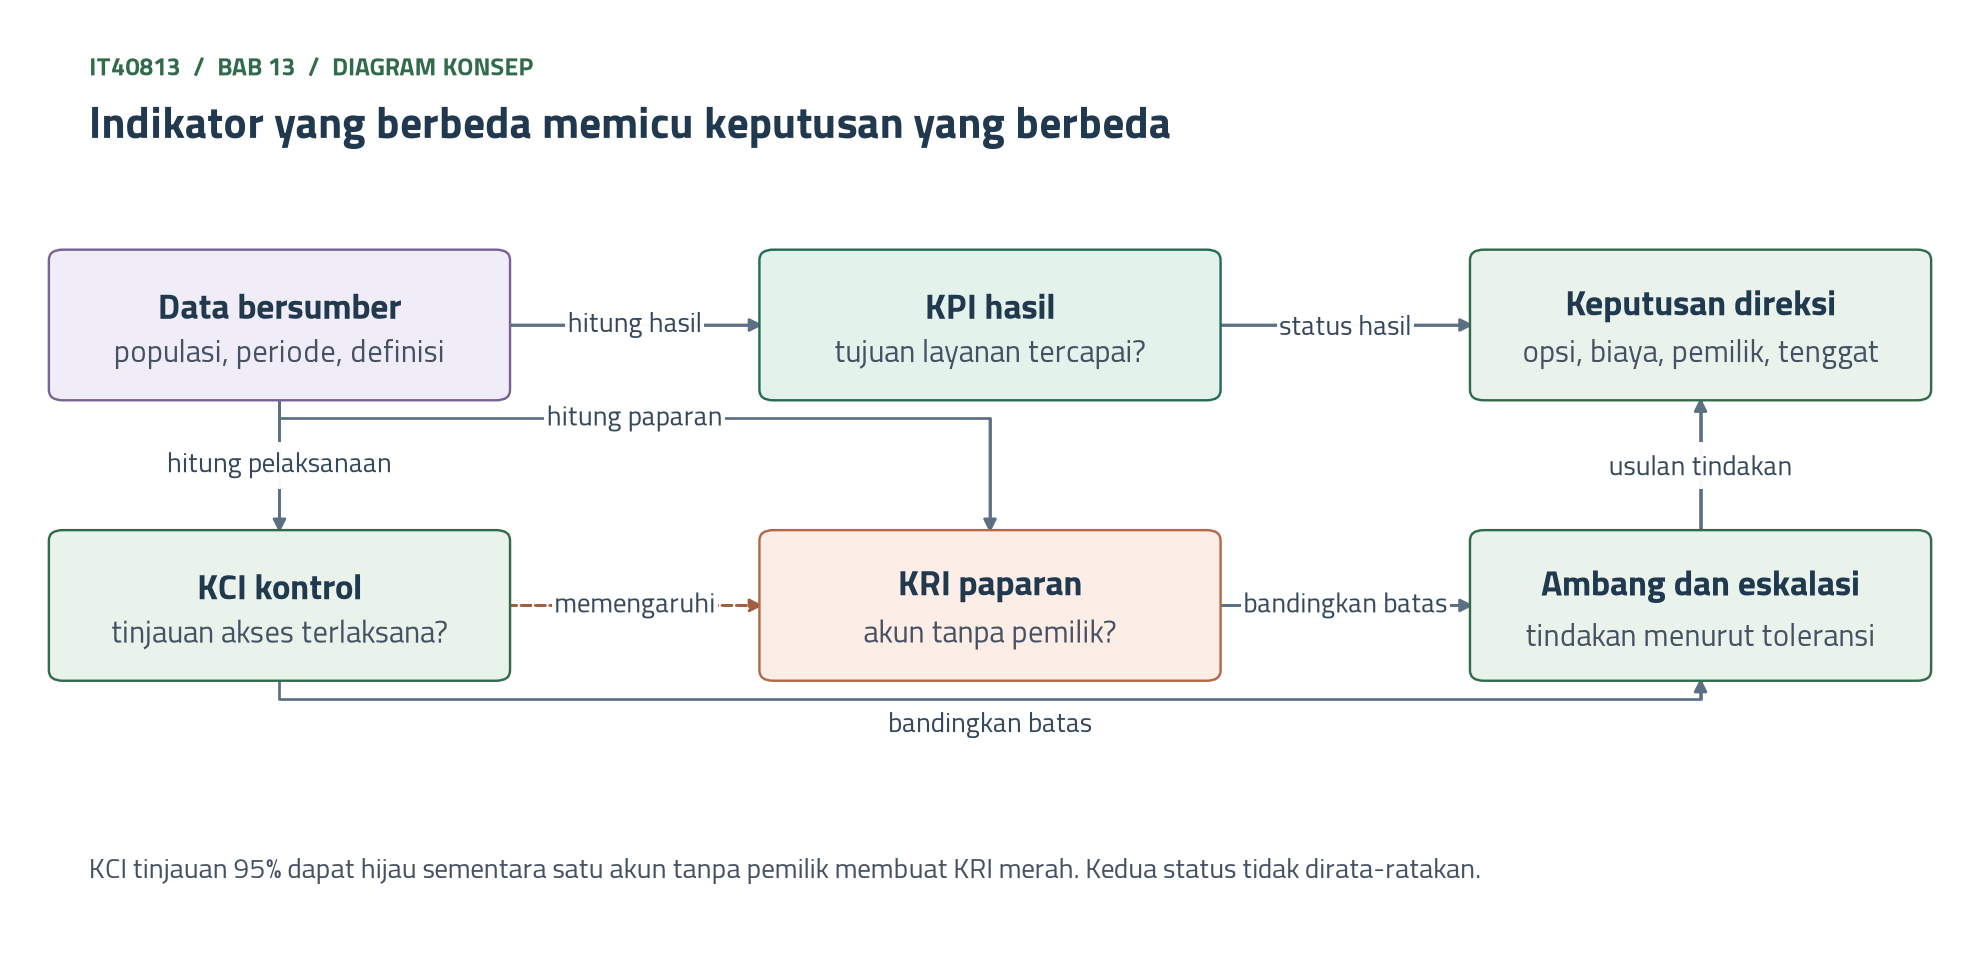
\includegraphics[width=\textwidth]{../figures/ch13-diagram-konsep.png}
  \caption{Indikator yang berbeda memicu keputusan yang berbeda}
  \label{fig:ch13-ilustrasi-bab}
\end{figure}
}{}

\section{KPI, KRI, dan KCI}

\subsection*{Tiga pertanyaan yang berbeda}

KPI menjawab apakah tujuan tercapai. KRI menjawab apakah paparan mendekati atau melewati batas.
KCI menjawab apakah kontrol dijalankan. COSO mengingatkan bahwa laporan kinerja sering berfokus
pada hasil yang sudah terjadi, sehingga belum tentu memberi peringatan dini. KRI dipakai untuk
memberi sinyal awal ketika paparan risiko meningkat \cite{c13-coso-kri}. Bab 5 mencatat fungsi
yang sama: ukuran seperti KRI menunjukkan bagian yang melewati toleransi atau yang masih berada
di dalamnya \cite{c05-nist-ir8286r1}.

Analogi kendaraan pengantar obat menunjukkan perbedaannya. Waktu tiba di apotek menunjukkan
hasil. Suhu mesin menunjukkan potensi gangguan. Buku servis rutin menunjukkan pelaksanaan kontrol.
Ketiganya membantu keputusan berbeda, dan tidak satu pun menggantikan yang lain.

Dua contoh pada Medikara:
\begin{enumerate}
  \item Misalkan 12 acara pelatihan keamanan hanya menjangkau 30 dari 100 pegawai prioritas, atau
  30 persen. Jumlah acara mengukur kegiatan. Cakupannya menunjukkan 70 pegawai belum terjangkau,
  dan itu pun belum membuktikan perilaku berubah.
  \item Misalkan 114 dari 120 akun vendor ditinjau tepat waktu pada Oktober 2026. KCI-nya 95 persen
  dan berstatus hijau. Pada bulan yang sama, 1 akun aktif belum memiliki pemilik. KRI-nya merah
  menurut batas nol pada Bab 5.
\end{enumerate}

Tabel~\ref{tab:ch13-jenis-indikator} merangkum ketiga jenis indikator beserta keputusan yang
dipicu.

\begin{table}[!htb]
  \centering\small
  \caption{Jenis indikator Medikara, Oktober 2026 (misalkan)}\label{tab:ch13-jenis-indikator}
  \begin{tabularx}{\textwidth}{|>{\raggedright\arraybackslash}p{0.08\textwidth}|>{\raggedright\arraybackslash}p{0.22\textwidth}|>{\raggedright\arraybackslash}X|>{\raggedright\arraybackslash}X|}
    \hline
    \textbf{Jenis} & \textbf{Pertanyaan} & \textbf{Ukuran contoh} & \textbf{Keputusan yang dipicu}
    \\ \hline
    KPI & Apakah hasil tercapai? & Waktu tunggu pendaftaran 28 menit, target 25 menit & Alur dan
    jadwal petugas diubah atau dipertahankan? \\ \hline
    KRI & Apakah paparan mendekati batas? & 1 akun vendor tanpa pemilik, batas 0 akun & Akun
    dibekukan atau diberi pengecualian darurat? \\ \hline
    KCI & Apakah kontrol dijalankan? & 114 dari 120 akun ditinjau tepat waktu & Daftar akun
    diperbaiki atau peninjau ditambah? \\ \hline
  \end{tabularx}
\end{table}

Dua hal pada indikator sering tertukar: KRI dan KCI. Pembagiannya begini. KCI mengukur pekerjaan
organisasi. KRI mengukur keadaan yang dihadapi organisasi. Cakupan peninjauan dapat mencapai 100
persen, sementara peninjau tetap menemukan akun tanpa pemilik. Klasifikasi mengikuti pertanyaan,
bukan nama datanya. Jumlah menit gangguan menjadi KRI bila dibandingkan dengan batas 2 jam per
bulan pada Bab 5. Data yang sama menjadi KPI bila kepala operasi TI memakainya untuk menilai
target waktu pulih.

Diagram konsep pada awal bab merangkum alurnya. Data bersumber memuat populasi, periode, dan
definisi. Dari data itu lahir KPI hasil, KCI kontrol, dan KRI paparan. Nilai dibandingkan dengan
batas pada ambang dan eskalasi, yaitu tindakan menurut toleransi. Status hasil dan usulan tindakan
lalu masuk ke keputusan direksi, yang memuat opsi, biaya, pemilik, dan tenggat.

Pertanyaan kemudian muncul: mengapa diagram itu memuat panah dari KCI ke KRI? Bab 5 memberi
angkanya. Pengandaian kasarnya: penurunan peluang R-01 sebanding dengan cakupan AC-01, dari 0,2
menuju 0,05. Hasilnya sebagai berikut:
\begin{enumerate}
  \item Cakupan 85 persen menghasilkan peluang $0{,}2 - 0{,}15 \times 0{,}85 = 0{,}0725$, dengan
  harapan kerugian Rp36,25 juta dari kerugian rata-rata Rp500 juta.
  \item Cakupan 90 persen menghasilkan peluang 0,065 dan harapan kerugian Rp32,5 juta, sama dengan
  Bab 5. Cakupan 95 persen menghasilkan 0,0575 dan Rp28,75 juta. Sasaran Rp25 juta baru tercapai
  pada cakupan penuh.
\end{enumerate}

Hubungan itu pengandaian, bukan hukum sebab akibat. Selisih 5 persen cakupan terakhir, yaitu 6
akun, bernilai Rp3,75 juta per tahun. Angka kecil itu tidak meniadakan kewajiban nol akun tanpa
pemilik, karena batas Bab 5 tidak ditetapkan dari harapan kerugian saja.

\begin{kasus}[title={Kasus Medikara Health: Indikator Hijau, Risiko Merah}]
Misalkan kepala operasi TI melaporkan cakupan AC-01 naik dari 85 persen menjadi 95 persen dalam
tiga bulan. Angka itu benar. Pemilik Medikara+ lalu membaca KRI pada halaman yang sama: 1 akun
vendor aktif belum memiliki pemilik. Angka ini juga benar, dan statusnya merah.

Keputusan membaca dua status secara terpisah punya dua konsekuensi. Pertama, perbaikan cakupan
tetap terlihat, sehingga kerja tim operasi tidak hilang dari laporan. Kedua, akun itu tetap
divalidasi dalam 1 hari kerja lalu dibekukan, walaupun hanya 1 dari 120 akun, atau sekitar 0,8
persen. Warna hijau pada satu baris tidak membayar warna merah pada baris lain.
\end{kasus}

\subsection*{Indikator yang mendahului dan yang tertinggal}

Indikator yang mendahului memberi peringatan sebelum kejadian. Indikator yang tertinggal
menggambarkan hasil sesudah kejadian. COSO menyarankan penelusuran mundur: dari kejadian risiko ke
kejadian antara, lalu ke akar penyebab. Data pada titik yang lebih awal berpotensi menjadi KRI yang
mendahului \cite{c13-coso-kri}. Makin dini sinyalnya, makin panjang waktu untuk bertindak.

Analogi prakiraan banjir membantu. Tinggi air di bendungan hulu memberi waktu mengungsi. Jumlah
rumah terendam hanya menghitung akibat. Keduanya berguna, tetapi hanya yang pertama dapat mencegah
kerugian pada hari itu.

Gambar~\ref{fig:ch13-rantai} menerapkan penelusuran itu pada R-01. Kode IK-01 sampai IK-12 adalah
indikator bab ini, yang dirinci pada seksi metrik.

\begin{figure}[!htb]
  \centering
  \begin{tikzpicture}[node distance=4.5mm, tahap/.style={draw, rounded corners, align=center, text width=2.4cm, minimum height=1.5cm, font=\scriptsize}, ukur/.style={draw, align=center, text width=2.4cm, minimum height=1.25cm, font=\scriptsize, fill=blue!8}, panah/.style={-{Stealth[length=2mm]}, thick}]
  \node[tahap,fill=blue!8] (a) {\textbf{Akar penyebab}\\[1pt]{\tiny\mdseries tanggal berakhir tidak masuk daftar}};
  \node[tahap,fill=orange!12] (b) [right=of a] {\textbf{Kejadian antara}\\[1pt]{\tiny\mdseries akun aktif melewati masa berlaku}};
  \node[tahap,fill=red!22] (c) [right=of b] {\textbf{Kejadian risiko}\\[1pt]{\tiny\mdseries akun membaca data pasien tanpa tugas}};
  \node[tahap,fill=gray!35] (d) [right=of c] {\textbf{Akibat}\\[1pt]{\tiny\mdseries pemberitahuan dan kerugian}};
  \draw[panah] (a) -- (b);
  \draw[panah] (b) -- (c);
  \draw[panah] (c) -- (d);
  \node[ukur] (ua) [below=6mm of a] {\textbf{KCI IK-07}\\{\tiny\mdseries cakupan peninjauan AC-01}};
  \node[ukur] (ub) [below=6mm of b] {\textbf{KRI IK-01, IK-02}\\{\tiny\mdseries akun tanpa pemilik; lewat masa berlaku}};
  \node[ukur] (uc) [below=6mm of c] {\textbf{Tinjauan \textit{log}}\\{\tiny\mdseries 247 dari 260 tinjauan mingguan (Bab 8)}};
  \node[ukur] (ud) [below=6mm of d] {\textbf{KPI IK-11}\\{\tiny\mdseries pemberitahuan tepat waktu}};
  \draw[-, dashed] (a) -- (ua);
  \draw[-, dashed] (b) -- (ub);
  \draw[-, dashed] (c) -- (uc);
  \draw[-, dashed] (d) -- (ud);
  \draw[panah] ([yshift=-5mm]ua.south west) -- node[below, font=\scriptsize] {sinyal makin terlambat, waktu untuk bertindak makin pendek} ([yshift=-5mm]ud.south east);
\end{tikzpicture}

  \caption{Rantai kejadian R-01 dan indikator pada tiap titik (misalkan)}
  \label{fig:ch13-rantai}
\end{figure}

Dua contoh membedakan keduanya:
\begin{enumerate}
  \item Bab 5 memberi contoh akun melewati masa berlaku naik dari 1 menjadi 5 dalam sebulan.
  Kenaikan itu memicu pemeriksaan sebelum insiden terulang. Indikator ini mendahului kejadian.
  \item Ketepatan pemberitahuan hanya memiliki nilai bila ada insiden wajib. Misalkan Agustus
  memuat 1 pemberitahuan yang tepat waktu, dan dua bulan berikutnya tidak ada. Indikator ini
  tertinggal. Ia tidak memberi peringatan, tetapi tetap perlu karena K-04 merupakan kewajiban.
\end{enumerate}

Hubungan waktu tidak otomatis membuktikan sebab akibat. Misalkan akun lewat masa berlaku turun 2,
1, 0 dan akun tanpa pemilik turun 3, 2, 1. Tiga titik data belum membuktikan yang satu menyebabkan
yang lain. COSO juga mengingatkan bahwa KRI tidak mengelola risiko, dan rancangan yang buruk dapat
memberi rasa aman palsu. Kemampuan prediksi tiap KRI karena itu dinilai terus-menerus
\cite{c13-coso-kri}.

\subsection*{Balanced Scorecard dan keseimbangan ukuran}

Kaplan dan Norton memperkenalkan Balanced Scorecard pada 1992. Alasannya, ukuran keuangan
tradisional dapat memberi sinyal yang menyesatkan bagi perbaikan berkelanjutan dan inovasi
\cite{c13-kaplan1992}. Rumusan umumnya menyandingkan empat perspektif: keuangan, pelanggan, proses
internal, serta inovasi dan pembelajaran. Teks utuh artikel tidak terbuka, sehingga daftar ini
tidak dikutip dari artikel. Bab ini tidak memakainya sebagai sistem
manajemen, melainkan sebagai pemeriksaan keseimbangan. Portofolio yang hanya berisi kontrol
keamanan tidak menjawab apakah pasien terlayani.

Analogi rapor sekolah menjelaskan gunanya. Nilai ujian, kehadiran, dan catatan perilaku dibaca
bersama. Nilai ujian tinggi dengan kehadiran 50 persen memberi pesan yang berbeda dari nilai yang
sama dengan kehadiran penuh.

Dua contoh ketidakseimbangan:
\begin{enumerate}
  \item Bab 2 mengandaikan investasi Rp8 miliar dengan kemajuan pekerjaan 90 persen, tetapi waktu
  tunggu hanya berubah dari 40 ke 38 menit. Capaian manfaatnya 2 dari 15 menit, atau 13,3 persen.
  Laporan proyek saja akan terlihat hijau.
  \item Misalkan waktu tunggu Oktober 28 menit. Capaian manfaatnya naik menjadi $12 \div 15 = 80$
  persen. Pada bulan yang sama, baru 1 dari 2 uji rumah sakit lulus. Layanan membaik, tetapi
  kesiapan pulihnya belum.
\end{enumerate}

Tabel~\ref{tab:ch13-keseimbangan} memeriksa keseimbangan portofolio Medikara. Kata ``pasien''
menggantikan ``pelanggan'' karena sesuai dengan konteks layanan.

\begin{table}[!htb]
  \centering\small
  \caption{Pemeriksaan keseimbangan portofolio Medikara, Oktober 2026 (misalkan)}
  \label{tab:ch13-keseimbangan}
  \begin{tabularx}{\textwidth}{|>{\raggedright\arraybackslash}p{0.19\textwidth}|>{\raggedright\arraybackslash}X|>{\raggedright\arraybackslash}p{0.13\textwidth}|>{\raggedright\arraybackslash}p{0.27\textwidth}|}
    \hline
    \textbf{Perspektif} & \textbf{Pertanyaan} & \textbf{Indikator} & \textbf{Nilai} \\ \hline
    Keuangan & Apakah peluang kerugian besar berada di dalam batas? & IK-04 & 1 skenario di atas
    batas 2 persen \\ \hline
    Pasien & Apakah layanan lebih cepat dan tersedia? & IK-03, IK-12 & 100 menit gangguan; tunggu
    28 menit \\ \hline
    Proses internal & Apakah kontrol berjalan dan bekerja? & IK-07, IK-08 & Cakupan 95 persen; 10
    dari 12 uji lulus \\ \hline
    Pembelajaran & Apakah temuan menghasilkan perbaikan yang teruji? & IK-10 & 9 dari 10 temuan
    tertutup \\ \hline
  \end{tabularx}
\end{table}

\section{Merancang Indikator yang Baik}

\subsection*{Kartu definisi}

NIST membedakan penilaian dari pengukuran. Penilaian mengevaluasi atau menimbang terhadap kriteria.
Pengukuran menghasilkan nilai kuantitatif. Metrik memakai hasil pengukuran untuk melacak kemajuan,
membantu keputusan, dan memperbaiki kinerja terhadap sasaran. Metrik yang bermakna bersifat
objektif, akurat, presisi, terikat pada titik waktu, dapat diulang, dan sebanding dengan pengukuran
sebelumnya. Dokumentasinya mencatat pihak yang bertanggung jawab, sumber data, dan bentuk laporan
\cite{c13-nist80055v1}. Volume 2 melanjutkannya menjadi program pengukuran \cite{c13-nist80055v2}.

Analogi nilai kelas menunjukkan bahaya penyebut yang kabur. Nilai rata-rata 90 berbeda maknanya
bila hanya menghitung siswa yang hadir, bukan seluruh peserta. Perubahan cara menghitung dapat
memperbaiki angka tanpa mengubah kemampuan kelas.

Dua contoh tentang penyebut:
\begin{enumerate}
  \item Bab 12 mencatat laporan unit TI berbunyi 108 dari 108 akun. Penyebut yang benar adalah 120
  akun pada daftar penugasan, sehingga cakupannya $108 / 120 = 90$ persen. Selisih 12 akun tidak
  pernah ditinjau. Kedua angka benar, tetapi hanya satu yang menjawab pertanyaan direksi.
  \item Misalkan sesudah perbaikan, pembilang diperketat menjadi akun yang ditinjau tepat waktu
  dalam bulan itu. Agustus menghasilkan $102 / 120 = 85$ persen, lebih rendah daripada 90 persen.
  Angka turun karena definisi menjadi lebih ketat, bukan karena kontrol memburuk. Perubahan definisi
  itu dicatat, dan tren lama tidak disambung tanpa catatan.
\end{enumerate}

Tabel~\ref{tab:ch13-definisi} memperlihatkan kartu definisi lengkap untuk satu indikator. Katalog
contoh seluruh indikator ada di \berkas{sources/chapter13/katalog-indikator.csv}.

\begin{table}[!htb]
  \centering\small
  \caption{Kartu definisi IK-07 Cakupan peninjauan AC-01 (misalkan)}\label{tab:ch13-definisi}
  \begin{tabularx}{\textwidth}{|>{\raggedright\arraybackslash}p{0.24\textwidth}|>{\raggedright\arraybackslash}X|}
    \hline
    \textbf{Unsur} & \textbf{Isi} \\ \hline
    Pertanyaan & Apakah peninjauan akses vendor dijalankan tepat waktu pada seluruh akun? \\ \hline
    Pembilang & Akun aktif yang ditinjau dalam bulan berjalan, dengan tanggal bukti \\ \hline
    Penyebut & Semua akun aktif pada daftar penugasan: 120 akun pada 5 rumah sakit \\ \hline
    Sumber & Daftar penugasan dan catatan peninjauan, bukan daftar dari sistem yang diperiksa \\
    \hline
    Frekuensi dan tanggal data & Bulanan; ekstrak pada hari kerja terakhir, versi disimpan \\ \hline
    Pemilik informasi & Kepala operasi TI sebagai pemilik tindakan \\ \hline
    Pengumpul dan penerima & Staf TI mengumpulkan; pemilik Medikara+ sebagai pemilik R-01 menerima
    \\ \hline
    Ambang & Minimal 95 persen hijau; 90 sampai kurang dari 95 kuning; kurang dari 90 merah \\
    \hline
    Tindakan & Periksa kelengkapan daftar akun; koreksi kuning dalam 5 hari kerja; merah dieskalasi
    \\ \hline
    Pemeriksa mutu & Audit internal mencocokkan sampel 30 akun (Bab 12) \\ \hline
  \end{tabularx}
\end{table}

\subsection*{Nol, kosong, dan tidak berlaku}

Tiga keadaan pada data sering tertukar. Pembagiannya begini. Nol yang sah berarti data lengkap dan
hasilnya nol. Tidak berlaku berarti penyebutnya nol karena kewajiban tidak muncul. Data tidak
tersedia berarti data kosong atau ekstrak tidak lengkap. Tabel~\ref{tab:ch13-keadaan} memberi
contohnya.

\begin{table}[!htb]
  \centering\small
  \caption{Tiga keadaan data pada \textit{dashboard} (misalkan)}\label{tab:ch13-keadaan}
  \begin{tabularx}{\textwidth}{|>{\raggedright\arraybackslash}p{0.2\textwidth}|>{\raggedright\arraybackslash}X|>{\raggedright\arraybackslash}p{0.3\textwidth}|}
    \hline
    \textbf{Keadaan} & \textbf{Contoh} & \textbf{Status} \\ \hline
    Nol yang sah & 0 baris kewajiban lewat tenggat pada Oktober, register lengkap & Dinilai menurut
    ambang: hijau \\ \hline
    Tidak berlaku & 0 pemberitahuan wajib pada September, sehingga penyebut nol & Tidak berlaku;
    bukan 100 persen \\ \hline
    Data tidak tersedia & Ekstrak akun Bogor gagal, sehingga 20 dari 120 akun tidak terbaca & Belum
    dapat dinilai; bukan hijau \\ \hline
  \end{tabularx}
\end{table}

Pembagian ini punya dua konsekuensi yang dapat dihitung. Pertama, ketepatan pemberitahuan tiga
bulan adalah 1 dari 1, bukan 3 dari 3. Menuliskan 100 persen untuk tiap bulan membuat dua bulan
tanpa kejadian terlihat seperti dua bukti keberhasilan. Kedua, bila ekstrak Bogor gagal, laporan
``nol akun tanpa pemilik'' hanya mencakup 100 dari 120 akun, atau 83,3 persen. Sebaran 120 akun
mengikuti Bab 12. Nol itu tidak dapat dibaca hijau.

\subsection*{Empat jenis ukuran menurut NIST}

NIST memakai pembagian lain: ukuran implementasi, efektivitas, efisiensi, dan dampak
\cite{c13-nist80055v1}. Ukuran implementasi memperlihatkan kemajuan kontrol, biasanya dalam
persentase, misalnya Multi-Factor Authentication (MFA) pada 108 dari 120 akun. Kontrol yang ada
belum tentu bekerja. Ukuran efektivitas menilai seberapa baik kontrol bekerja, misalnya 29 dari 36
uji pemulihan lulus. Ukuran efisiensi melihat ketepatan waktu kontrol, misalnya akun dicabut paling
lambat 1 hari kerja. Ukuran dampak menyatakan akibat bagi misi, misalnya harapan kerugian R-01
Rp28,75 juta, yang masih bergantung pada pengandaian Bab 5.

Dua pembagian itu menjawab hal berbeda. KPI, KRI, dan KCI menjelaskan pertanyaan yang dijawab. Jenis
NIST menjelaskan apa yang diukur. NIST menyarankan urutan: sesudah ukuran implementasi tersedia,
organisasi memprioritaskan ukuran lain berdasarkan strategi risiko, tujuan, ketersediaan data, nilai
aset, biaya kontrol, dan kewajiban \cite{c13-nist80055v1}.

\section{Ambang Batas dan Eskalasi}

\subsection*{Menurunkan ambang dari batas Bab 5}

Ambang menerjemahkan \textit{risk appetite} menjadi tindakan. COSO menyebutnya titik pemicu: tingkat
yang ditetapkan sebelumnya beserta rencana tindakan \cite{c13-coso-kri}. CSF mencatat hal yang
berkaitan pada GV.RM-02: pernyataan \textit{risk appetite} dan \textit{risk tolerance} ditetapkan,
dikomunikasikan, dan dipelihara \cite{nistcsf2}. Batas tidak tumpang tindih dan mencakup seluruh
nilai yang valid. Pemilik, waktu tindakan, dan jalur eskalasi ditetapkan sebelum pengukuran. Merah
tidak selalu berarti penghentian, karena respons mengikuti risiko dan kewenangan.

Analogi alarm tangki air menunjukkan perlunya waktu merespons. Peringatan muncul sebelum air habis.
Alarm yang berbunyi setelah keran kering sudah terlambat memberi kesempatan bertindak.

Tabel~\ref{tab:ch13-ambang} menurunkan KRI dari lima batas pada Bab 5. Ambang kuning ditambahkan
hanya bila ada ruang di dalam batas. Pada IK-03, ruang itu berasal dari Recovery Time Objective
(RTO) Bab 10.

\begin{table}[!htb]
  \centering\small
  \caption{Lima batas Bab 5 menjadi ambang KRI (misalkan)}\label{tab:ch13-ambang}
  \begin{tabularx}{\textwidth}{|>{\raggedright\arraybackslash}X|>{\raggedright\arraybackslash}p{0.11\textwidth}|>{\raggedright\arraybackslash}p{0.25\textwidth}|>{\raggedright\arraybackslash}p{0.23\textwidth}|}
    \hline
    \textbf{Batas Bab 5} & \textbf{KRI} & \textbf{Ambang} & \textbf{Tindakan} \\ \hline
    Kerahasiaan: nol akun vendor aktif tanpa pemilik dan masa berlaku & IK-01, IK-02 & 0 hijau;
    lebih dari 0 merah & Validasi 1 hari kerja, lalu bekukan \\ \hline
    Kelangsungan: pendaftaran terganggu paling lama 2 jam per bulan & IK-03 & Paling lama 90 menit
    hijau; lebih dari 90 sampai 120 kuning; lebih dari 120 merah & Pemilik layanan menyiapkan
    perbaikan; merah memicu tinjauan mingguan \\ \hline
    Finansial: peluang kerugian Rp1,5 miliar atau lebih paling tinggi 2 persen per tahun per
    skenario & IK-04 & 0 skenario hijau; lebih dari 0 merah & Laporkan ke komite pengarah TI dan
    komite risiko \\ \hline
    Kepatuhan: K-01 sampai K-16 berpemilik; nol baris lewat tenggat tanpa keputusan & IK-05 & 0
    hijau; lebih dari 0 merah & Catat penyimpangan dan tindakan \\ \hline
    Keselamatan: risiko cedera berat ditinjau dalam 1 hari kerja & IK-06 & 0 laporan terlambat
    hijau; lebih dari 0 merah & Libatkan pimpinan klinis segera \\ \hline
  \end{tabularx}
\end{table}

Dua contoh memperlihatkan penurunannya:
\begin{enumerate}
  \item IK-03 memakai dua angka lama. Batas Bab 5 adalah 120 menit per bulan. RTO pendaftaran Bab
  10 adalah 90 menit, sehingga satu kejadian yang memenuhi target masih menyisakan 30 menit.
  Misalkan Agustus 150 menit, September 40 menit, dan Oktober 100 menit. Bab 5 menghitung 2 jam
  gangguan menyentuh sekitar 548 kunjungan, sehingga 150 menit menyentuh sekitar 685 kunjungan dan
  100 menit sekitar 457 kunjungan.
  \item IK-04 memakai perkalian pada Bab 5 dan Bab 8. Peluang R-01 dikali 0,2 menghasilkan 1,45,
  1,3, dan 1,15 persen pada tiga bulan, semuanya di dalam batas 2 persen. R-05 tetap dicatat 0,1
  selama syarat opsi B pada Bab 10 belum terpenuhi, sehingga peluang kerugian Rp1,5 miliar atau
  lebih 10 persen. Nilai IK-04 karena itu 1 skenario pada ketiga bulan.
\end{enumerate}

Gambar~\ref{fig:ch13-ambang-gambar} memperlihatkan ketiga bulan IK-03 pada zona ambangnya.

\begin{figure}[!htb]
  \centering
  \begin{tikzpicture}[x=0.062cm, y=1cm, panah/.style={-{Stealth[length=2mm]}, thick}, zona/.style={draw, minimum height=0.8cm, font=\scriptsize\bfseries}, titik/.style={circle, fill=black, inner sep=1.6pt}]
  % Zona dibaca dari batas Bab 5 dan RTO Bab 10, satu satuan x sama dengan satu menit.
  \fill[green!10] (0,0) rectangle (90,0.8);
  \fill[orange!12] (90,0) rectangle (120,0.8);
  \fill[red!22] (120,0) rectangle (180,0.8);
  \draw (0,0) rectangle (180,0.8);
  \draw (90,0) -- (90,0.8);
  \draw (120,0) -- (120,0.8);
  \node[font=\scriptsize\bfseries] at (45,0.4) {Hijau};
  \node[font=\scriptsize\bfseries] at (105,0.4) {Kuning};
  \node[font=\scriptsize\bfseries] at (150,0.4) {Merah};
  \draw[panah] (0,-0.08) -- (186,-0.08) node[right, font=\scriptsize] {menit};
  \foreach \menit in {0,90,120,180} {
    \draw (\menit,-0.14) -- (\menit,-0.02);
    \node[below, font=\scriptsize] at (\menit,-0.14) {\menit};
  }
  \node[below, align=center, text width=2.5cm, font=\tiny] at (82,-0.48) {RTO pendaftaran\\(Bab 10)};
  \node[below, align=center, text width=2.5cm, font=\tiny] at (128,-0.48) {Batas 2 jam per bulan\\(Bab 5)};
  \node[titik] (ags) at (150,0.8) {};
  \node[titik] (sep) at (40,0.8) {};
  \node[titik] (okt) at (100,0.8) {};
  \node[above, align=center, font=\scriptsize] at (ags.north) {Agustus\\150};
  \node[above, align=center, font=\scriptsize] at (sep.north) {September\\40};
  \node[above, align=center, font=\scriptsize] at (okt.north) {Oktober\\100};
\end{tikzpicture}

  \caption{Zona ambang IK-03 dari RTO Bab 10 dan batas Bab 5 (misalkan)}
  \label{fig:ch13-ambang-gambar}
\end{figure}

Toleransi nol punya dua konsekuensi. Pertama, tren membaik tidak mengubah warna. Akun tanpa pemilik
3, 2, 1 tetap merah sampai nol. Zona kuning buatan akan melunakkan batas yang sudah disahkan
direksi. Kedua, peringatan dini berpindah ke indikator lain. IK-02 dan IK-07 memberi waktu sebelum
akun kehilangan pemilik. Pengecualian darurat Bab 5 ditulis tegas dalam definisi: akun dengan
pengecualian yang sah dicatat terpisah selama belum 24 jam. Sesudah itu, akun masuk hitungan IK-01.

Periode waktu juga memengaruhi tafsir. Rata-rata tiga bulan IK-03 adalah $290 \div 3 \approx 96{,}7$
menit, dan berada pada zona kuning. Rata-rata itu menyembunyikan pelanggaran 150 menit pada Agustus.
Karena batas Bab 5 berbunyi per bulan, status dibaca per bulan. Jumlah tahunan dibandingkan dengan
24 jam, atau 1.440 menit, sebagai pembacaan tambahan.

\subsection*{Aturan tepi dan populasi kecil}

Pertanyaan berikutnya: bagaimana bila nilai tepat berada pada batas? Aturan tepi ditulis sejak awal.
Nilai 95 persen termasuk hijau, 90 persen termasuk kuning, dan 120 menit termasuk kuning. Status
memakai nilai sebelum pembulatan, karena pembulatan dapat memindahkan warna. Pada IK-07, satu akun
bernilai sekitar 0,83 persen.

Dua contoh menunjukkan akibatnya:
\begin{enumerate}
  \item Misalkan cakupan turun dari 115 menjadi 113 akun. Nilainya turun dari 95,83 menjadi 94,17
  persen, sehingga status berubah menjadi kuning. Koreksi 5 hari kerja berjalan ketika jarak ke
  merah masih 6 akun, karena merah dimulai pada 107 akun.
  \item Pada populasi kecil, satu butir mengubah banyak persen. Medikara memiliki 5 penilaian
  dampak pelindungan data, atau Data Protection Impact Assessment (DPIA), pada Bab 7, sehingga satu
  butir bernilai 20 persen. Ambang kuning 90 persen tidak dapat dicapai tanpa menjadi hijau. Ambang
  kuning karena itu ditulis 80 persen.
\end{enumerate}

Ambang juga diuji pada data lalu sebelum dipakai. Misalkan kuning IK-03 dimulai pada 30 menit.
Ketiga bulan tidak ada yang hijau, sehingga sinyal berbunyi setiap bulan dan cepat diabaikan. Dengan
ambang 90 menit, tiga bulan itu menghasilkan satu hijau, satu kuning, dan satu merah. Tiga titik
belum cukup untuk menyimpulkan ambang tepat, tetapi cukup untuk menolak ambang yang selalu berbunyi.

\subsection*{Jalur eskalasi}

Eskalasi menjawab siapa yang harus bertindak ketika ambang terlewati, dan kapan. COSO mencatat bahwa
direksi tidak perlu mengetahui seluruh KRI, tetapi perlu mengikuti KRI untuk paparan risiko teratas.
Laporan pengecualian dapat dibuat berkala, dengan waktu yang berbeda menurut tingkat penerimanya
\cite{c13-coso-kri}. Tabel~\ref{tab:ch13-eskalasi} memakai batas delegasi Bab 2, sehingga jalur
indikator tidak membuat wewenang baru.

\begin{table}[!htb]
  \centering\small
  \caption{Jalur eskalasi indikator Medikara (misalkan)}\label{tab:ch13-eskalasi}
  \begin{tabularx}{\textwidth}{|>{\raggedright\arraybackslash}p{0.2\textwidth}|>{\raggedright\arraybackslash}X|>{\raggedright\arraybackslash}p{0.3\textwidth}|}
    \hline
    \textbf{Tingkat} & \textbf{Pemicu} & \textbf{Waktu} \\ \hline
    Pemilik tindakan & Nilai kuning atau merah & Merah 1 hari kerja; kuning 5 hari kerja \\ \hline
    Pemilik risiko & Merah belum tertutup; butuh pengecualian & Hari kerja berikutnya; pengecualian
    paling lama 24 jam \\ \hline
    Kepala TI & Perbaikan butuh biaya sampai Rp100 juta & Ringkasan triwulan ke komite \\ \hline
    Komite pengarah TI & Biaya di atas Rp100 juta sampai Rp400 juta; merah dua bulan berturut-turut
    & Rapat bulanan \\ \hline
    Direksi & Biaya di atas Rp400 juta sampai Rp5 miliar; penerimaan risiko di atas batas & Laporan
    triwulan, atau segera bila pemicu krisis organisasi terpenuhi \\ \hline
    Dewan komisaris & Di atas Rp5 miliar, bila anggaran dasar menetapkan & Laporan triwulan \\
    \hline
  \end{tabularx}
\end{table}

Dua jalur memerlukan pengecualian dari urutan itu. IK-06 langsung melibatkan pimpinan klinis, tanpa
menunggu tingkat di bawahnya. Pemberitahuan pada K-04 mengikuti jam insiden pada Bab 7, bukan jadwal
rapat. Jalur umum tidak boleh memperlambat kewajiban yang punya tenggat sendiri.

\begin{kasus}[title={Kasus Medikara Health: Satu Akun pada Oktober}]
Misalkan ekstrak Oktober menemukan 1 akun vendor tanpa pemilik. Kepala operasi TI memvalidasinya
dalam 1 hari kerja. Akun itu milik teknisi pada penugasan yang sudah dipindahkan ke unit lain.
Pemilik Medikara+ memilih membekukan akun, dan menolak pengecualian 24 jam karena tidak ada
pekerjaan darurat.

Keputusan ini punya dua konsekuensi. Pertama, teknisi yang masih bertugas perlu meminta akun baru
melalui penugasan yang benar, sehingga pekerjaannya tertunda 1 hari kerja. Kedua, IK-01 tetap merah
pada laporan Oktober, walaupun akun sudah dibekukan. Nilai yang dilaporkan adalah keadaan pada
tanggal data. Status dapat menjadi hijau pada periode berikutnya bila ekstrak lengkap dan hasilnya
nol. Rekonsiliasi lanjutan sampai Rp60 juta berada di bawah batas Rp100 juta, sehingga kepala TI
yang memutuskan.
\end{kasus}

\section{Metrik Tata Kelola, Keamanan, dan Privasi}

\subsection*{Portofolio dua belas indikator}

Portofolio indikator mencakup tata kelola, risiko, keamanan, privasi, dan kelangsungan layanan.
Ukuran dipilih dari pertanyaan direksi, bukan dari data yang mudah dikumpulkan. NIST mengingatkan
kecenderungan memakai semua data yang tersedia. Metrik yang salah pilih merusak mutu laporan dan
kepercayaan pada hasil kerja. Ujinya: apakah data itu langsung menggambarkan kinerja kontrol yang
sah, atau melacak risiko yang material? Bila tidak, data itu sebaiknya dikeluarkan. Pada tahap awal,
lebih sedikit sering lebih baik \cite{c13-nist80055v1}.

Analogi pemeriksaan kesehatan rutin menjelaskan pilihan itu. Dokter membaca tekanan darah, gula
darah, dan kolesterol, bukan seluruh angka yang dapat dihasilkan laboratorium. Tiap angka memiliki
batas dan tindak lanjut. Angka tanpa tindak lanjut hanya menambah kecemasan.

Dua contoh tentang angka yang perlu dilengkapi:
\begin{enumerate}
  \item Bab 10 mencatat 29 dari 36 uji pemulihan lulus, atau 80,6 persen. Pada 5 rumah sakit yang
  menjalankan Sistem Informasi Manajemen Rumah Sakit (SIMRS), hanya 3 yang lulus, atau 60 persen.
  Dua kegagalan data seluruhnya berasal dari 9 uji akun terpisah. Angka gabungan perlu dilengkapi
  identitas layanan yang gagal, karena dampaknya tidak setara.
  \item Bab 9 mencatat 5 hubungan vendor tingkat terperinci. Misalkan 4 dari 5 sudah dinilai ulang,
  atau 80 persen. Hubungan yang belum dinilai dilaporkan beserta akses datanya. Bila hubungan itu
  V-01 dengan skor 9, angka 80 persen menyembunyikan vendor yang paling berisiko.
\end{enumerate}

Tabel~\ref{tab:ch13-portofolio} memuat portofolio contoh. Kolom pemilik menyebut pemilik tindakan.
Pemilik risiko tetap mengikuti register Bab 5, sehingga keduanya dipisahkan seperti pada Bab 6.
Ambang keenam KRI mengikuti Tabel~\ref{tab:ch13-ambang}, dan rincian lainnya ada di katalog.

\begin{table}[!htb]
  \centering\small
  \caption{Portofolio dua belas indikator Medikara (misalkan)}\label{tab:ch13-portofolio}
  \begin{tabularx}{\textwidth}{|>{\raggedright\arraybackslash}p{0.08\textwidth}|>{\raggedright\arraybackslash}X|>{\raggedright\arraybackslash}p{0.07\textwidth}|>{\raggedright\arraybackslash}p{0.2\textwidth}|>{\raggedright\arraybackslash}p{0.2\textwidth}|}
    \hline
    \textbf{Kode} & \textbf{Indikator} & \textbf{Jenis} & \textbf{Pemilik tindakan} &
    \textbf{Kaitan} \\ \hline
    IK-01 & Akun vendor aktif tanpa pemilik atau masa berlaku & KRI & Kepala operasi TI & R-01,
    AC-01 \\ \hline
    IK-02 & Akun melewati masa berlaku & KRI & Kepala operasi TI & R-01, AC-01 \\ \hline
    IK-03 & Menit gangguan pendaftaran & KRI & Kepala operasi TI & R-03, R-05 \\ \hline
    IK-04 & Skenario melewati batas peluang kerugian & KRI & Kepala risiko & R-01, R-05 \\ \hline
    IK-05 & Baris kewajiban lewat tenggat tanpa keputusan & KRI & Fungsi kepatuhan & K-01 sampai
    K-16 \\ \hline
    IK-06 & Risiko cedera berat lewat tinjauan 1 hari kerja & KRI & Pimpinan klinis & R-11 \\ \hline
    IK-07 & Cakupan peninjauan AC-01 & KCI & Kepala operasi TI & R-01, AC-01 \\ \hline
    IK-08 & Uji pemulihan lulus, gabungan dan rumah sakit & KCI & Kepala operasi TI & R-05, K-02 \\
    \hline
    IK-09 & DPIA selesai & KCI & Petugas pelindungan data & 5 DPIA Bab 7 \\ \hline
    IK-10 & Temuan tertutup tepat waktu sesudah uji ulang & KPI & Pemilik tiap temuan & TA-01 dan
    lainnya \\ \hline
    IK-11 & Pemberitahuan tepat waktu & KPI & Petugas pelindungan data & R-12, K-04 \\ \hline
    IK-12 & Waktu tunggu pendaftaran 18 klinik & KPI & Kepala pendaftaran & Target Bab 1 dan Bab 2
    \\ \hline
  \end{tabularx}
\end{table}

COBIT dan CSF memberi bahasa pengawasan untuk portofolio itu. Dalam susunan COBIT 2019, MEA01
menangani pemantauan kinerja dan kesesuaian oleh manajemen, sedangkan EDM05 menangani keterlibatan
pemangku kepentingan \cite{c04-gmo}. Uraian ini umum, dan perlu dicocokkan ke naskah ISACA sebelum
dipakai untuk audit. CSF memiliki GV.OV-03: kinerja pengelolaan risiko keamanan siber dievaluasi dan
ditinjau untuk penyesuaian yang diperlukan \cite{nistcsf2}. Bab 8 menargetkan GV.RM-02 terbukti
lewat batas yang diuji dengan satu penyimpangan. Akun Oktober dapat menjadi bukti ujinya. Skor
buatan organisasi tidak menjadi sertifikasi NIST.

Portofolio juga berarti ada yang dikeluarkan. Keputusan ini punya dua konsekuensi. Pertama,
``perubahan disetujui'' dan ``hubungan vendor dinilai'' tetap dipantau, tetapi pada tingkat forum.
Kedua, privasi di tingkat direksi hanya terwakili IK-09 dan IK-11. Sesudah 5 DPIA selesai, IK-09
kehilangan daya beda, dan penggantinya dibahas pada tinjauan tahunan. COSO juga mengingatkan bahwa
KRI kehilangan nilai ketika tujuan dan strategi berubah \cite{c13-coso-kri}.

\subsection*{Mengolah bahan dari Bab 8 sampai Bab 12}

Bab-bab sebelumnya sudah menghasilkan banyak angka. Pertanyaan kemudian muncul: angka mana yang naik
ke direksi? Tabel~\ref{tab:ch13-bahan} memilahnya menurut tingkat pembaca. Bab 9 menyerahkan enam
indikator hubungan terperinci, dan seluruhnya tercatat di sini. Hanya satu yang langsung masuk
portofolio.

\begin{table}[!htb]
  \centering\small
  \caption{Bahan indikator dari Bab 8 sampai Bab 12 (misalkan)}\label{tab:ch13-bahan}
  \begin{tabularx}{\textwidth}{|>{\raggedright\arraybackslash}p{0.08\textwidth}|>{\raggedright\arraybackslash}X|>{\raggedright\arraybackslash}p{0.27\textwidth}|>{\raggedright\arraybackslash}p{0.16\textwidth}|}
    \hline
    \textbf{Asal} & \textbf{Bahan} & \textbf{Diolah menjadi} & \textbf{Pembaca} \\ \hline
    Bab 8 & T-19: 247 dari 260 tinjauan \textit{log} mingguan, atau 95 persen & KCI jejak aktivitas
    & Komite pengarah TI \\ \hline
    Bab 9 & Akun vendor tanpa pemilik, 0 akun & IK-01 & Direksi bila merah \\ \hline
    Bab 9 & Catatan AC-01, 60 dari 60 per tahun atau 5 per bulan & Rincian IK-07 & Pemilik risiko \\
    \hline
    Bab 9 & Laporan dugaan insiden vendor 12 jam, K-05 & Masuk IK-05 bila lewat tenggat tanpa
    keputusan & Komite risiko \\ \hline
    Bab 9 & Latihan bersama 2 per tahun; subprosesor 30 hari; uji ekspor 1 per tahun & Kalender
    kontrol: selesai atau belum & Pengelola vendor \\ \hline
    Bab 10 & RTO 90 menit; 29 dari 36 uji; 3 dari 5 rumah sakit & IK-03, IK-08 & Direksi \\ \hline
    Bab 11 & 27 dari 30 kasus darurat tertangkap; 93 dari 120 tanda klinik keliru; AI-03 selisih 8,
    ambang 5 & KCI mutu kecerdasan artifisial (AI); jalur penyebab R-11 pada IK-06, tanpa kode baru
    & Komite risiko \\ \hline
    Bab 12 & TA-01; 24 dari 30 akun sesuai; kriteria 30 dari 30 & IK-10; pemeriksa mutu IK-07 &
    Direksi bila lewat tenggat \\ \hline
  \end{tabularx}
\end{table}

\begin{kasus}[title={Kasus Medikara Health: Dari 46 Usulan menjadi 12 Indikator}]
Misalkan tiap unit mengusulkan ukuran kesayangannya, dan terkumpul 46 usulan. Kepala risiko memakai
tiga pertanyaan: keputusan apa yang dipicu, batas mana yang dipakai, dan siapa pemiliknya. Sebanyak
19 usulan gugur karena tidak memicu keputusan, misalnya jumlah tiket yang dibuka. Sebanyak 15 usulan
tetap dipantau di tingkat operasional. Sisanya 12 indikator.

Pilihan ini punya biaya. Unit yang ukurannya keluar merasa pekerjaannya tidak terlihat. COSO
mencatat bahwa pakar di unit dapat cenderung memilih metrik yang sudah biasa dipakai
\cite{c13-coso-kri}. Kepala risiko karena itu mencatat alasan setiap penolakan, dan membuka tinjauan
ulang setiap tahun.
\end{kasus}

\subsection*{Metrik platform dan SLO}

Ukuran layanan dari IT40713 dan nilai platform dari IT40613 menjadi masukan risiko. Service Level
Objective (SLO) adalah sasaran tingkat layanan. SLO berbeda dari batas hukum dan \textit{risk
appetite}, dan rinciannya dibahas pada kedua mata kuliah itu. Bab 9 memberi contoh: layanan pesan
tersedia 99,5 persen dari 8.760 jam, atau terganggu 43,8 jam per tahun. Batas pendaftaran Bab 5
adalah 24 jam dari 4.380 jam layanan. Dasar hitungnya berbeda, sehingga kedua angka tidak digabung
menjadi satu persentase ketersediaan.

\section{Mutu Data dan Risiko Manipulasi}

\subsection*{Sumber data dan mutu data}

Indikator hanya sebaik datanya. NIST meminta cara pengumpulan dan tempat penyimpanan data
didefinisikan dengan jelas. Validitas data patut diragukan bila sumber utamanya hanya menyimpan
laporan dari sebagian unit, atau proses pelaporan antarunit tidak konsisten. Pemeriksaan integritas,
akurasi, dan struktur dijalankan sebelum analisis \cite{c13-nist80055v1}. COSO menambahkan bahwa
tanpa keseragaman cara ukur, data gabungan kehilangan kekuatan dan menambah gangguan pada keputusan
\cite{c13-coso-kri}.

Analogi timbangan pasar membantu. Harga per kilogram antarkios tidak dapat dibandingkan bila
timbangannya berbeda. Tera ulang menjadi syarat perbandingan, sebelum ada yang berdebat soal harga.

Sektor lain sudah merasakan akibatnya. Basel Committee on Banking Supervision mencatat bahwa krisis
keuangan sejak 2007 memperlihatkan banyak bank tidak mampu menggabungkan paparan risiko secara
penuh, cepat, dan akurat, lalu menerbitkan prinsip agregasi data dan pelaporan risiko
\cite{c13-bcbs239}. Prinsip itu tidak mengikat Medikara, tetapi pelajarannya tetap berlaku.

Dua contoh pada Medikara:
\begin{enumerate}
  \item Bab 8 mengandaikan laporan 18 klinik tidak konsisten karena definisi indikator berbeda.
  Dengan 2 jam rekonsiliasi per klinik per bulan, pekerjaannya 432 jam per tahun, atau Rp25,92 juta.
  IK-12 menuntut satu definisi: kapan tunggu dimulai dan kapan selesai.
  \item Register Bab 5 memuat R-04, versi spreadsheet yang berbeda menghasilkan angka salah.
  Peluangnya 0,5 dan kerugiannya Rp60 juta, sehingga harapan kerugiannya Rp30 juta per tahun.
  Spreadsheet boleh dipakai untuk \textit{dashboard} awal, asalkan versi dan sumbernya tercatat.
\end{enumerate}

Tabel~\ref{tab:ch13-mutu} menempatkan pemeriksaan mutu pada lima sumber data. Pemeriksa tidak
berasal dari pihak yang menghasilkan angka, mengikuti temuan Bab 12 bahwa daftar tidak boleh diambil
dari sistem yang diperiksa.

\begin{table}[!htb]
  \centering\small
  \caption{Sumber data dan pemeriksaan mutu (misalkan)}\label{tab:ch13-mutu}
  \begin{tabularx}{\textwidth}{|>{\raggedright\arraybackslash}p{0.13\textwidth}|>{\raggedright\arraybackslash}X|>{\raggedright\arraybackslash}X|>{\raggedright\arraybackslash}p{0.19\textwidth}|}
    \hline
    \textbf{Indikator} & \textbf{Sumber} & \textbf{Pemeriksaan} & \textbf{Pemeriksa} \\ \hline
    IK-01, IK-07 & Daftar penugasan dan inventaris identitas & Jumlah 120 cocok; 5 rumah sakit
    terbaca & Audit internal, sampel \\ \hline
    IK-03 & Catatan gangguan & Dicocokkan dengan laporan loket pendaftaran & Kepala pendaftaran \\
    \hline
    IK-08 & Catatan uji pemulihan & Rumah sakit dan fasilitas lain dipisah; hasil disahkan & Pemilik
    layanan \\ \hline
    IK-10 & Sistem pelacakan temuan & Hanya status sesudah uji ulang yang dihitung & Audit internal
    \\ \hline
    IK-12 & Catatan antrean 18 klinik & Definisi mulai dan selesai sama; klinik kosong ditandai &
    Fungsi data klinik \\ \hline
  \end{tabularx}
\end{table}

\subsection*{Indikator yang dimanipulasi}

Indikator dengan target mengubah perilaku orang yang diukur. Bevan dan Hood menelaah tata kelola
lewat target pada layanan kesehatan publik Inggris. Mereka berpendapat bahwa cara itu mengandaikan
bagian dapat mewakili keseluruhan, serta mengandaikan masalah pengukuran dan \textit{gaming} tidak
penting. Bukti dari layanan kesehatan dipakai untuk menguji kedua pengandaian itu
\cite{c13-bevan2006}. \textit{Gaming} di sini berarti pengubahan perilaku atau catatan supaya angka
terlihat baik, tanpa perbaikan yang setara.

Analogi kasir warung menjelaskan mekanismenya. Bila kasir dinilai dari jumlah struk, satu belanjaan
dapat dipecah menjadi tiga struk. Angkanya naik, dan penjualan tidak berubah. Kasir itu tidak perlu
berniat jahat, karena ukuran sudah mendorongnya ke sana.

Dua contoh dengan angka:
\begin{enumerate}
  \item Misalkan gangguan pendaftaran 125 menit memuat 40 menit yang dicatat sebagai pemeliharaan.
  Nilainya turun menjadi 85 menit, dan status merah berubah menjadi hijau. Pasien tetap mengantre
  125 menit. Definisi IK-03 karena itu mengukur akibat pada pendaftaran, bukan sebab gangguan.
  \item Misalkan 10 temuan dilaporkan selesai menurut manajemen, tetapi hanya 9 yang lolos uji
  ulang. Bila status pertama dihitung, IK-10 menjadi 100 persen. Bila status kedua dihitung,
  nilainya 90 persen. Bab 12 sudah memisahkan keduanya, dan TA-01 berada pada baris yang belum
  tertutup.
\end{enumerate}

Tabel~\ref{tab:ch13-manipulasi} merangkum bentuk yang sering muncul. Daftar ini disusun bab ini
sebagai alat bantu, bukan rangkuman artikel Bevan dan Hood.

\begin{table}[!htb]
  \centering\small
  \caption{Bentuk manipulasi indikator dan pengamannya}\label{tab:ch13-manipulasi}
  \begin{tabularx}{\textwidth}{|>{\raggedright\arraybackslash}p{0.2\textwidth}|>{\raggedright\arraybackslash}X|>{\raggedright\arraybackslash}X|}
    \hline
    \textbf{Bentuk} & \textbf{Contoh} & \textbf{Pengaman} \\ \hline
    Mengecilkan penyebut & 12 akun keluar dari daftar, 90 menjadi 100 persen & Populasi dari daftar
    penugasan; jumlah dicocokkan \\ \hline
    Memindahkan kategori & Insiden wajib dicatat tidak wajib, IK-11 menjadi tidak berlaku & Alasan
    klasifikasi ditinjau fungsi hukum \\ \hline
    Menutup di atas kertas & Temuan selesai menurut manajemen dihitung tertutup & Hitung sesudah uji
    ulang \\ \hline
    Mengejar batas & Peninjauan tergesa pada akhir bulan supaya tepat 95 persen & Sampel mutu;
    catatan per akun \\ \hline
    Mengubah definisi & Tepat waktu digeser dari 30 menjadi 45 hari & Riwayat definisi; tren tidak
    disambung \\ \hline
  \end{tabularx}
\end{table}

Pilihan pengaman punya \textit{tradeoff}. Pemeriksaan sampel menambah kerja, tetapi Bab 12 sudah
menyediakan kapasitas audit 1.800 jam per tahun, sehingga pemeriksaan mutu masuk rencana itu.
Mengaitkan indikator dengan bonus memperkuat perhatian, tetapi juga memperkuat dorongan untuk
memanipulasi. Pada Medikara, KRI dengan toleransi nol tidak dikaitkan dengan bonus. Unit yang jujur
melaporkan 1 akun tanpa pemilik tidak boleh dirugikan dibanding unit yang tidak memeriksanya.

\section{Dashboard dan Prinsip Visualisasi}

Few mendefinisikan \textit{dashboard} sebagai tampilan visual dari informasi terpenting untuk
mencapai tujuan tertentu, disatukan dalam satu layar sehingga dapat dipantau sekilas. Isinya
terutama ringkasan tingkat tinggi beserta pengecualian. \textit{Dashboard} memberi tahu apa yang
terjadi, bukan mengapa \cite{c13-few2004}. COSO mencatat warna hijau, kuning, dan merah lazim
dipakai untuk menandai status KRI pada laporan direksi \cite{c13-coso-kri}. Warna disertai angka dan
label, supaya status tetap terbaca pada cetakan hitam putih.

Analogi papan keberangkatan stasiun menjelaskan perannya. Papan itu menyebut kereta, jam, dan status
terlambat. Penumpang dapat segera memutuskan. Alasan keterlambatan dicari di tempat lain, dan papan
tidak mencoba memuatnya.

Bab ini memakai prinsip sederhana yang disusun dari rujukan di atas, bukan daftar resmi. Satu
halaman cukup, dan rincian disimpan di katalog. Pengecualian ditaruh lebih dahulu. Warna selalu
disertai angka dan kata status. Tiga nilai terakhir terlihat. Tanggal data ditulis, dan perubahan
definisi diberi catatan. Tidak ada hiasan, jarum, atau rata-rata warna.

Gambar~\ref{fig:ch13-dashboard} memperlihatkan \textit{dashboard} Oktober. Baris terkecil pada tiap
petak adalah nilai Agustus, September, dan Oktober. Tabel~\ref{tab:ch13-tren} menyajikan angka yang
sama secara lengkap, dan hasilnya dapat dicek ulang di
\berkas{sources/chapter13/dashboard-contoh.csv}.

\begin{figure}[!htb]
  \centering
  \begin{tikzpicture}[petak/.style={draw, rounded corners=1pt, align=center, text width=2.55cm, minimum height=2.05cm, font=\scriptsize, execute at begin node={\hyphenpenalty=10000}}]
  % Baris disusun dari pengecualian: merah lebih dahulu, lalu kuning, hijau, dan tidak berlaku.
  \node[petak,fill=red!22] at (0,0) {\textbf{IK-01 Akun tanpa pemilik}\\{\footnotesize\textbf{1 akun}}\\MERAH\\{\tiny\mdseries 3, 2, 1}};
  \node[petak,fill=red!22] at (2.85,0) {\textbf{IK-04 Skenario lewat batas}\\{\footnotesize\textbf{1 (R-05)}}\\MERAH\\{\tiny\mdseries 1, 1, 1}};
  \node[petak,fill=red!22] at (5.7,0) {\textbf{IK-08 Uji pemulihan}\\{\footnotesize\textbf{83,3\%}}\\MERAH\\{\tiny\mdseries rumah sakit 1 dari 2}\\{\tiny\mdseries 75\%, 83,3\%, 83,3\%}};
  \node[petak,fill=orange!12] at (8.55,0) {\textbf{IK-03 Gangguan pendaftaran}\\{\footnotesize\textbf{100 menit}}\\KUNING\\{\tiny\mdseries 150, 40, 100}};
  \node[petak,fill=orange!12] at (0,-2.15) {\textbf{IK-12 Waktu tunggu}\\{\footnotesize\textbf{28 menit}}\\KUNING\\{\tiny\mdseries 34, 31, 28}};
  \node[petak,fill=green!10] at (2.85,-2.15) {\textbf{IK-02 Lewat masa berlaku}\\{\footnotesize\textbf{0 akun}}\\HIJAU\\{\tiny\mdseries 2, 1, 0}};
  \node[petak,fill=green!10] at (5.7,-2.15) {\textbf{IK-05 Kewajiban lewat tenggat}\\{\footnotesize\textbf{0 baris}}\\HIJAU\\{\tiny\mdseries 2, 1, 0}};
  \node[petak,fill=green!10] at (8.55,-2.15) {\textbf{IK-06 Cedera lewat tinjauan}\\{\footnotesize\textbf{0 laporan}}\\HIJAU\\{\tiny\mdseries 0, 1, 0}};
  \node[petak,fill=green!10] at (0,-4.3) {\textbf{IK-07 Cakupan AC-01}\\{\footnotesize\textbf{95\%}}\\HIJAU\\{\tiny\mdseries 85\%, 90\%, 95\%}};
  \node[petak,fill=green!10] at (2.85,-4.3) {\textbf{IK-09 DPIA selesai}\\{\footnotesize\textbf{100\%}}\\HIJAU\\{\tiny\mdseries 60\%, 80\%, 100\%}};
  \node[petak,fill=green!10] at (5.7,-4.3) {\textbf{IK-10 Temuan tertutup}\\{\footnotesize\textbf{90\%}}\\HIJAU\\{\tiny\mdseries 60\%, 80\%, 90\%}};
  \node[petak,fill=gray!35] at (8.55,-4.3) {\textbf{IK-11 Pemberitahuan}\\{\footnotesize\textbf{Nol kewajiban}}\\TIDAK BERLAKU\\{\tiny\mdseries 100\%, lalu tidak berlaku}};
\end{tikzpicture}

  \caption{\textit{Dashboard} GRC Medikara, Oktober 2026 (misalkan)}
  \label{fig:ch13-dashboard}
\end{figure}

\begin{table}[!htb]
  \centering\small
  \caption{Tren dua belas indikator, Agustus sampai Oktober 2026 (misalkan)}\label{tab:ch13-tren}
  \begin{tabularx}{\textwidth}{|>{\raggedright\arraybackslash}X|>{\raggedright\arraybackslash}p{0.22\textwidth}|>{\raggedright\arraybackslash}p{0.22\textwidth}|>{\raggedright\arraybackslash}p{0.22\textwidth}|}
    \hline
    \textbf{Indikator} & \textbf{Agustus} & \textbf{September} & \textbf{Oktober} \\ \hline
    IK-01 Akun tanpa pemilik & 3, merah & 2, merah & 1, merah \\ \hline
    IK-02 Lewat masa berlaku & 2, merah & 1, merah & 0, hijau \\ \hline
    IK-03 Gangguan pendaftaran & 150 menit, merah & 40 menit, hijau & 100 menit, kuning \\ \hline
    IK-04 Skenario lewat batas & 1, merah & 1, merah & 1, merah \\ \hline
    IK-05 Kewajiban lewat tenggat & 2, merah & 1, merah & 0, hijau \\ \hline
    IK-06 Cedera lewat tinjauan & 0, hijau & 1, merah & 0, hijau \\ \hline
    IK-07 Cakupan AC-01 & 102/120 = 85\%, merah & 108/120 = 90\%, kuning & 114/120 = 95\%, hijau
    \\ \hline
    IK-08 Uji pemulihan & 9/12 = 75\%; rumah sakit 1/2, merah & 10/12 = 83,33\%; rumah sakit 1/1,
    kuning & 10/12 = 83,33\%; rumah sakit 1/2, merah \\ \hline
    IK-09 DPIA selesai & 3/5 = 60\%, merah & 4/5 = 80\%, kuning & 5/5 = 100\%, hijau \\ \hline
    IK-10 Temuan tertutup & 6/10 = 60\%, merah & 8/10 = 80\%, kuning & 9/10 = 90\%, hijau \\ \hline
    IK-11 Pemberitahuan & 1/1 = 100\%, hijau & Tidak berlaku & Tidak berlaku \\ \hline
    IK-12 Waktu tunggu & 34 menit, merah & 31 menit, merah & 28 menit, kuning \\ \hline
  \end{tabularx}
\end{table}

IK-08 memakai status terburuk dari dua rasio, dengan ambang yang sama: 100 persen hijau, 75 sampai
kurang dari 100 persen kuning, dan kurang dari 75 persen merah. Pada Oktober, 83,33 persen berstatus
kuning, tetapi rumah sakit 1 dari 2 atau 50 persen berstatus merah. Pembacaan ini mengikuti
peringatan Bab 10: gabungan menyamarkan layanan dengan batas gangguan terpendek. Dua belas uji per
bulan membentuk 36 uji triwulan, dengan 29 lulus, sama dengan Bab 10.

Pertanyaan kemudian muncul: bolehkah semua warna dirangkum menjadi satu skor? Dua contoh
menjawabnya:
\begin{enumerate}
  \item Misalkan hijau bernilai 100, kuning 50, merah 0, dan tidak berlaku dikeluarkan. Skor
  gabungannya 16,7 pada Agustus, 27,3 pada September, dan $700 \div 11 \approx 63{,}6$ pada Oktober.
  Skor naik hampir empat kali lipat, sementara IK-01 dan IK-04 merah pada ketiga bulan. Oktober
  bahkan memuat kegagalan uji rumah sakit.
  \item Cakupan AC-01 hijau dan akun tanpa pemilik merah tidak dirata-ratakan menjadi kuning.
  Rata-rata itu tidak berarti apa-apa bagi pemilik Medikara+, karena tidak menunjukkan akun mana
  yang dibekukan.
\end{enumerate}

Bab 5 sudah membahas keterbatasan kategori pada matriks risiko, termasuk resolusi yang buruk
\cite{c05-cox2008}. Skor gabungan warna mewarisi masalah yang sama. Keputusan menolak skor gabungan
punya konsekuensi: laporan bertambah satu baris untuk tiap pengecualian, dan pimpinan tidak mendapat
satu angka yang mudah diingat. Harga itu diterima, karena pesan yang hilang justru pesan yang
dibutuhkan.

\section{Laporan Satu Halaman ke Direksi}

\subsection*{Struktur laporan}

Laporan menghubungkan tiga pesan utama dengan satu keputusan. NIST mengingatkan bahwa ukuran yang
dilaporkan tanpa konteks dapat menimbulkan akibat yang tidak diinginkan atau keraguan. Laporan
karena itu dapat memuat risiko yang ditunjukkan ukuran, kesesuaiannya dengan \textit{risk appetite},
tindakan atau keputusan yang diperlukan, masalah kepatuhan, dan dampaknya pada kesiapan audit
\cite{c13-nist80055v1}. COSO menambahkan bahwa frekuensi mengikuti pembacanya. Pengelola operasi
cocok dengan laporan seketika, manajemen senior dengan laporan yang lebih jarang, dan direksi dengan
laporan yang lebih agregat \cite{c13-coso-kri}. Pada Medikara, \textit{dashboard} dibahas bulanan
pada komite pengarah TI, dan laporan satu halaman terbit triwulanan sesuai 4 laporan pada Bab 2.

Analogi ringkasan rapat membedakan informasi dan keputusan. Daftar kejadian menjelaskan masa lalu.
Usulan dengan pemilik, anggaran, tenggat, dan risiko sisa memberi dasar bertindak.

Dua contoh tentang isi laporan:
\begin{enumerate}
  \item Misalkan laporan menyebut 7 kegiatan selesai. Direksi belum mengetahui dampak, pengecualian,
  dan keputusan yang diperlukan. Membaca 7 baris itu pun tidak mengubah apa pun.
  \item Misalkan laporan meminta direksi menyetujui Rp60 juta untuk rekonsiliasi akun. Permintaan
  itu salah alamat. Bab 2 menempatkan biaya sampai Rp100 juta pada kepala TI, sehingga cukup
  dilaporkan. Waktu direksi dipakai untuk Rp180 juta tahap kedua opsi B, karena keputusan bersyarat
  itu milik direksi pada Bab 10.
\end{enumerate}

Gambar~\ref{fig:ch13-laporan} memperlihatkan susunan satu halaman. Keputusan ditaruh di atas, karena
itu hal pertama yang perlu diketahui pembaca.

\begin{figure}[!htb]
  \centering
  \begin{tikzpicture}[blok/.style={draw, align=left, text width=7.1cm, font=\scriptsize, inner sep=3pt}, catatan/.style={align=left, text width=3.5cm, font=\scriptsize, execute at begin node={\hyphenpenalty=10000}}, panah/.style={-{Stealth[length=2mm]}, thick}]
  \node[blok,fill=praditagreen!15] (kepala) {\textbf{Laporan GRC Triwulan Agustus sampai Oktober 2026}\\{\tiny\mdseries Cakupan, tanggal data, penyusun, dan pemilik laporan}};
  \node[blok,fill=orange!12,below=1.5mm of kepala] (putus) {\textbf{Keputusan yang diminta}\\{\tiny\mdseries Setujui, ubah, atau tolak: tahap kedua Rp180 juta untuk opsi B, paling lambat akhir November 2026}};
  \node[blok,fill=blue!8,below=1.5mm of putus] (p1) {\textbf{Pesan 1: Pemulihan belum memenuhi syarat}\\{\tiny\mdseries 3 dari 5 rumah sakit lulus; R-05 masih 10 persen, batasnya 2 persen}};
  \node[blok,fill=blue!8,below=1mm of p1] (p2) {\textbf{Pesan 2: Akses vendor membaik, belum selesai}\\{\tiny\mdseries Cakupan 95 persen; 1 akun tanpa pemilik dibekukan; TA-01 belum tertutup}};
  \node[blok,fill=blue!8,below=1mm of p2] (p3) {\textbf{Pesan 3: Layanan membaik, masih di bawah target}\\{\tiny\mdseries Waktu tunggu 34, 31, 28 menit; gangguan 150, 40, 100 menit}};
  \node[blok,fill=blue!8,below=1.5mm of p3] (opsi) {\textbf{Tabel tiga pilihan}\\{\tiny\mdseries Biaya, akibat pada risiko, pemilik, tenggat, dan ukuran keberhasilan}};
  \node[blok,fill=green!10,below=1.5mm of opsi] (batas) {\textbf{Batas data dan tindak lanjut}\\{\tiny\mdseries Tingkat lulus uji bukan peluang R-05; 5 uji rumah sakit tergolong sedikit}};
  \draw (kepala.north west) rectangle (batas.south east);
  \node[catatan,right=4mm of putus] (c1) {Dibaca pertama: direksi tahu apa yang harus diputuskan};
  \node[catatan,right=4mm of p2] (c2) {Tiga pesan: angka, tren, dan risiko; tanpa daftar kegiatan};
  \node[catatan,right=4mm of opsi] (c3) {Ada pembanding, sehingga usulan dapat ditolak};
  \node[catatan,right=4mm of batas] (c4) {Batas klaim mencegah tafsir berlebihan};
  \draw[panah] (c1.west) -- (putus.east);
  \draw[panah] (c2.west) -- (p2.east);
  \draw[panah] (c3.west) -- (opsi.east);
  \draw[panah] (c4.west) -- (batas.east);
\end{tikzpicture}

  \caption{Susunan laporan GRC satu halaman (misalkan)}
  \label{fig:ch13-laporan}
\end{figure}

\subsection*{Laporan Medikara: triwulan Agustus sampai Oktober 2026}

Hubungan antarangka berjalan seperti ini. IK-08 memperlihatkan 3 dari 5 rumah sakit lulus. Dua
kegagalan data berasal dari 9 uji akun terpisah. Kedua syarat Bab 10 belum terpenuhi. Peluang R-05
tetap dicatat 0,1, sehingga IK-04 merah. Tingkat lulus uji bukan peluang R-05, sehingga angka 80,6
persen tidak dibaca sebagai peluang apa pun. Tabel~\ref{tab:ch13-keputusan} menyusun pilihannya.

\begin{table}[!htb]
  \centering\small
  \caption{Tiga pilihan untuk tahap kedua opsi B (misalkan)}\label{tab:ch13-keputusan}
  \begin{tabularx}{\textwidth}{|>{\raggedright\arraybackslash}p{0.26\textwidth}|>{\raggedright\arraybackslash}p{0.13\textwidth}|>{\raggedright\arraybackslash}X|>{\raggedright\arraybackslash}X|}
    \hline
    \textbf{Pilihan} & \textbf{Biaya} & \textbf{Akibat pada R-05} & \textbf{Risiko pilihan} \\
    \hline
    1. Tahan tahap kedua; uji ulang 2 rumah sakit dan 9 uji akun terpisah & Rp0 tambahan saat ini &
    Peluang tetap 0,1; harapan kerugian sekitar Rp40 juta lebih tinggi per triwulan & Direksi
    menerima tertulis paparan di atas batas selama satu triwulan \\ \hline
    2. Cairkan Rp180 juta sekarang & Rp180 juta & Peluang tetap dicatat 0,1 sampai uji lulus &
    Syarat direksi hilang; uang keluar sebelum bukti \\ \hline
    3. Hentikan opsi B, kembali ke opsi A & Hemat Rp180 juta & SIMRS pulih 480 menit; batas 2 persen
    dilanggar & Sudah ditolak pada Bab 10 \\ \hline
  \end{tabularx}
\end{table}

\begin{kasus}[title={Kasus Medikara Health: Laporan yang Meminta Satu Keputusan}]
Misalkan kepala risiko menyusun laporan triwulan pada November 2026.

\textbf{Pesan 1.} Pemulihan belum memenuhi syarat. Sebanyak 29 dari 36 uji lulus, tetapi hanya 3
dari 5 rumah sakit. Dua kegagalan data berasal dari 9 uji akun terpisah. R-05 masih 10 persen,
batasnya 2 persen.

\textbf{Pesan 2.} Akses vendor membaik, tetapi belum selesai. Cakupan AC-01 naik 85, 90, 95 persen.
Satu akun tanpa pemilik sudah dibekukan. TA-01 selesai menurut manajemen, dan belum lolos uji ulang.
Tidak ada keputusan yang diminta, karena biayanya berada dalam wewenang kepala TI.

\textbf{Pesan 3.} Layanan membaik, dan masih di bawah target. Waktu tunggu 34, 31, 28 menit, dengan
target 25 menit. Gangguan pendaftaran Oktober 100 menit, di dalam batas 120 menit, tetapi di atas
RTO 90 menit.

\textbf{Keputusan yang diminta.} Setujui pilihan 1 paling lambat akhir November 2026. Pemilik
tindakan kepala operasi TI. Ukuran keberhasilan: 5 dari 5 rumah sakit lulus uji SIMRS di bawah 120
menit, dan 9 dari 9 uji akun terpisah berhasil, paling lambat akhir Januari 2027.

Selisih harapan kerugian R-05 antara 0,1 dan 0,02 adalah Rp160 juta per tahun, atau sekitar Rp40
juta per triwulan. Angka itu harga menunggu bukti. Direksi dapat menolaknya, asalkan penolakan
beserta risiko sisanya dicatat. Bab 14 memasukkan opsi B Rp480 juta ke peta jalan.
\end{kasus}

Laporan yang lebih pendek juga mengubah beban kerja. Tabel~\ref{tab:ch13-beban} menghitungnya pada
tarif Rp60.000 per jam dari Bab 7. Misalkan laporan lama melibatkan 8 unit dengan 6 jam per bulan,
ditambah penyunting 16 jam. Rancangan baru memerlukan 2 jam per indikator per bulan dan 24 jam per
laporan triwulan.

\begin{table}[!htb]
  \centering\small
  \caption{Beban laporan lama dan rancangan baru (misalkan)}\label{tab:ch13-beban}
  \begin{tabularx}{\textwidth}{|>{\raggedright\arraybackslash}X|>{\raggedright\arraybackslash}p{0.27\textwidth}|>{\raggedright\arraybackslash}p{0.27\textwidth}|}
    \hline
    \textbf{Unsur} & \textbf{Laporan 40 halaman} & \textbf{Satu halaman} \\ \hline
    Penyusunan per tahun & $(8 \times 6 + 16) \times 12 = 768$ jam & $12 \times 2 \times 12 + 4
    \times 24 = 384$ jam \\ \hline
    Biaya per tahun & Rp46,08 juta & Rp23,04 juta \\ \hline
    Waktu baca per pembaca & 80 menit, 12 kali & Sekitar 5 menit, 4 kali \\ \hline
  \end{tabularx}
\end{table}

Keputusan mengganti laporan punya dua konsekuensi. Pertama, penghematan 384 jam atau Rp23,04 juta
per tahun berarti indikator ini tidak menambah beban 3.046 jam yang harus dimuat Bab 14. Kedua,
sebagian pembaca kehilangan rincian yang biasa diterima. Rincian itu tetap tersedia di
\textit{dashboard} dan katalog, dan dibaca oleh pihak yang memang bertugas memakainya.

\section{Aktivitas: Dashboard KPI dan KRI serta Laporan Satu Halaman}

\textbf{Tujuan.} Tim menyediakan laporan yang memicu tindakan: katalog 8 sampai 12 indikator,
\textit{dashboard} sederhana, dan laporan satu halaman untuk direksi Medikara atau organisasi tim.

\textbf{Pembagian peran.} Analis risiko memimpin penetapan ambang dan memastikan KRI memakai batas
Bab 5. Anggota berlatar bisnis menyusun narasi untuk direksi. Analis teknologi memeriksa
ketersediaan dan mutu data. Pemilik konteks memastikan penerima laporan memiliki kewenangan atas
keputusan yang diminta.

\textbf{Langkah kerja.}
\begin{enumerate}
  \item Pilih 8 sampai 12 indikator yang mencakup tata kelola, risiko, keamanan, privasi, dan
  kelangsungan layanan. Tulis keputusan yang didukung tiap ukuran. Ukuran tanpa keputusan
  dikeluarkan.
  \item Isi katalog mengikuti kolom \berkas{sources/chapter13/katalog-indikator.csv}. Tetapkan
  rumus, sumber, frekuensi, pemilik, serta ambang tiga warna yang tidak tumpang tindih.
  \item Hitung tiga periode dari \berkas{sources/chapter13/data-indikator.csv}, atau dari data
  organisasi yang sudah dianonimkan. Bedakan nol yang sah, tidak berlaku, dan data tidak tersedia.
  \item Bandingkan hasil dengan \berkas{sources/chapter13/dashboard-contoh.csv}, lalu susun
  \textit{dashboard} pada spreadsheet. Cantumkan angka, kata status, tren, dan perubahan definisi.
  \item Tulis tiga pesan dan satu keputusan melalui
  \berkas{sources/chapter13/templat-laporan-direksi.md}. Nyatakan pilihan, biaya, pemilik, tenggat,
  dan risiko bila ditunda.
  \item Tinjau silang rumus antaranggota, lalu simulasikan rapat 5 menit. Catat apakah direksi
  fiktif dapat memilih tindakan tanpa bertanya apa yang diminta.
\end{enumerate}

\textbf{Luaran.} Katalog indikator, \textit{dashboard}, dan laporan satu halaman.

\textbf{Kaitan dengan capstone.} Luaran masuk tonggak C4 Peta Jalan dan Tata Kelola. Bab 14 memakai
indikator ini sebagai ukuran keberhasilan peta jalan. Metrik layanan diselaraskan dengan IT40713,
dan nilai platform diselaraskan dengan IT40613.

\textbf{Kriteria penilaian.} Kaitan risiko dan keputusan 30 persen; ketepatan definisi dan hitungan
30 persen; ambang dan eskalasi 20 persen; kejelasan permintaan keputusan 20 persen. Hasil tiap tim
boleh berbeda dari contoh. Penilaian berfokus pada penalaran.

\textbf{Berkas pendukung.} Daftar lengkap ada di \berkas{sources/chapter13/README.md}. Data
organisasi nyata wajib seizin organisasi dan dianonimkan. Data pribadi pasien atau karyawan tidak
boleh dipakai.

\begin{pendalaman}
Skrip \texttt{hitung\_indikator.py} menghitung 12 indikator dari data sintetis secara lokal.
Listing~\ref{lst:ch13-status} memperlihatkan aturan penyebut nol dan pembulatan. Nilai penuh
dibandingkan dengan ambang, lalu baru dibulatkan untuk tampilan.

\begin{lstlisting}[basicstyle=\ttfamily\scriptsize,columns=fullflexible,frame=lines,breaklines=true,
  caption={Status rasio, tersedia di \berkas{sources/chapter13/hitung_indikator.py}},
  label={lst:ch13-status}]
def status_rasio(pembilang, penyebut, batas_hijau, batas_kuning):
  """Bandingkan nilai penuh sebelum pembulatan agar ambang tidak bergeser."""
  if pembilang is None or penyebut is None:
    return None, DATA_TIDAK_TERSEDIA
  if pembilang > penyebut:
    raise ValueError("Pembilang melebihi penyebut")
  if penyebut == 0:
    return None, TIDAK_BERLAKU
  nilai = pembilang / penyebut * 100
  if nilai >= batas_hijau:
    return nilai, HIJAU
  if nilai >= batas_kuning:
    return nilai, KUNING
  return nilai, MERAH
\end{lstlisting}

Tim dapat mengotomasi pengambilan dua indikator dari sumber data nyata, misalnya sistem tiket atau
\textit{log}, ke alat \textit{dashboard} sumber terbuka seperti Metabase atau Grafana. Otomasi
memerlukan definisi dan pemeriksaan mutu yang sama. Pengambilan data hanya untuk sistem sendiri atau
yang sudah berizin tertulis. Keberhasilan mengambil data belum membuktikan indikator tepat untuk
keputusan.
\end{pendalaman}

\section{Ringkasan}

KPI, KRI, dan KCI menjawab pertanyaan tentang hasil, paparan, dan kontrol. Data yang sama dapat
mendukung beberapa keputusan bila definisi dan batas tafsirnya jelas. Cakupan AC-01 yang naik sampai
95 persen tidak meniadakan 1 akun tanpa pemilik. Indikator yang mendahului memberi waktu untuk
bertindak, sedangkan indikator yang tertinggal mencatat hasil yang tetap perlu dipertanggungjawabkan
secara terbuka.

Indikator yang baik memiliki pembilang, penyebut, cakupan, tanggal, sumber, pemilik, dan tindakan.
Perbedaan 108 dari 108 dengan 108 dari 120 berasal dari penyebut, bukan dari pekerjaan. Data tidak
tersedia dan penyebut nol tidak boleh diperlakukan sebagai kinerja sempurna. Mutu data diperiksa
oleh pihak di luar penghasil angka, karena ukuran dengan target mendorong orang menyesuaikan
catatan.

Ambang diturunkan dari batas Bab 5 dan memberi waktu merespons. Tidak semua indikator memerlukan
tiga warna. Toleransi nol tetap merah sampai nol, sehingga peringatan dini berpindah ke indikator
lain. Pada IK-03, RTO 90 menit dan batas 120 menit membentuk zona kuning yang berasal dari keputusan
terdahulu. Jalur eskalasi mengikuti batas delegasi Bab 2, sehingga indikator tidak menciptakan
wewenang baru.

Portofolio 12 indikator dipilih dari 46 usulan pada contoh Medikara, dan bahan Bab 8 sampai Bab 12
dipilah menurut pembacanya. \textit{Dashboard} menunjukkan keadaan, tren, dan pengecualian pada satu
halaman, tanpa skor gabungan. Skor 63,6 pada Oktober terlihat membaik, padahal dua KRI merah pada
ketiga bulan dan satu KCI gagal pada rumah sakit.

Laporan direksi mengajukan pilihan yang dapat diputuskan. Medikara tidak meminta persetujuan Rp60
juta yang berada dalam wewenang kepala TI, tetapi meminta keputusan atas Rp180 juta tahap kedua opsi
B, dengan harga menunggu sekitar Rp40 juta per triwulan. Pesan utama bab ini: indikator berguna
ketika mengubah keputusan dan tindakan, bukan ketika memenuhi halaman laporan.

\section{Latihan}

\subsection*{Latihan 1: Aktivitas atau Risiko}

``Jumlah pelatihan keamanan yang diselenggarakan'' diusulkan sebagai KRI. Kritisi usulan ini dan
tawarkan indikator yang lebih baik. Latihan ini membuktikan bahwa ukuran kegiatan belum tentu
menggambarkan paparan risiko. NIST memberi arah serupa: pelatihan kesadaran keamanan dinilai dari
tingkat penyelesaian dan hasil kuis, bukan dari label partisipasi rendah, sedang, atau tinggi
\cite{c13-nist80055v1}.
\begin{enumerate}
  \item Tetapkan risiko dan perilaku yang hendak diubah.
  \item Bandingkan jumlah acara dengan cakupan dan hasil uji.
  \item Usulkan rumus, ambang, dan keputusan yang dipicunya.
\end{enumerate}

Tabel~\ref{tab:ch13-lat1-contoh} memberi contoh terisi, dan Tabel~\ref{tab:ch13-lat1-hasil} menjadi
lembar isian.

\begin{table}[!htb]
  \centering\small
  \caption{Contoh terisi Latihan 1 (misalkan)}\label{tab:ch13-lat1-contoh}
  \begin{tabularx}{\textwidth}{|>{\raggedright\arraybackslash}X|>{\raggedright\arraybackslash}p{0.25\textwidth}|>{\raggedright\arraybackslash}X|}
    \hline
    \textbf{Ukuran} & \textbf{Nilai contoh} & \textbf{Batas tafsir} \\ \hline
    Pelatihan diselenggarakan & 12 acara & Tidak menunjukkan siapa belajar \\ \hline
    Cakupan pegawai prioritas & $30 / 100 = 30$ persen & Hadir belum berarti paham \\ \hline
    Peserta lulus uji & $24 / 30 = 80$ persen & Hanya berlaku bagi peserta \\ \hline
    Usulan KRI: pegawai prioritas belum lulus dalam 12 bulan & $100 - 24 = 76$ pegawai & Memicu
    penjadwalan; belum membuktikan perilaku \\ \hline
  \end{tabularx}
\end{table}

\begin{table}[!htb]
  \centering\small
  \caption{Lembar isian Latihan 1}\label{tab:ch13-lat1-hasil}
  \begin{tabularx}{\textwidth}{|>{\raggedright\arraybackslash}X|>{\raggedright\arraybackslash}p{0.25\textwidth}|>{\raggedright\arraybackslash}X|}
    \hline
    \textbf{Ukuran} & \textbf{Nilai} & \textbf{Batas tafsir} \\ \hline
    \dots & \dots & \dots \\ \hline
    \dots & \dots & \dots \\ \hline
    \dots & \dots & \dots \\ \hline
  \end{tabularx}
\end{table}

Hasil dapat berbeda. Penilaian bertumpu pada alasan dan perbandingan bukti.
\begin{enumerate}
  \item Pada contoh, mengapa 80 persen lulus uji tidak berarti 80 persen pegawai prioritas
  terlindungi?
  \item Data apa yang diperlukan sebelum menyimpulkan risiko turun?
  \item Bagaimana mencegah target mendorong manipulasi jumlah peserta?
\end{enumerate}

\subsection*{Latihan 2: Menurunkan Ambang Akses}

Turunkan ambang KRI untuk risiko kontrol akses dari pernyataan \textit{risk appetite} yang dibuat
pada Pertemuan 5. Latihan ini membuktikan bahwa toleransi, ambang, dan eskalasi harus konsisten.
\begin{enumerate}
  \item Salin pernyataan toleransi dan cakupannya dari luaran Pertemuan 5.
  \item Tentukan nilai yang melewati toleransi, pemilik, dan tindakan.
  \item Tetapkan indikator pendamping yang memberi peringatan dini.
  \item Uji ambang pada tiga periode.
\end{enumerate}

Tabel~\ref{tab:ch13-lat2-contoh} memberi contoh terisi dari batas nol akun pada Bab 5, dan
Tabel~\ref{tab:ch13-lat2-hasil} menjadi lembar isian.

\begin{table}[!htb]
  \centering\small
  \caption{Contoh terisi Latihan 2 (misalkan)}\label{tab:ch13-lat2-contoh}
  \begin{tabularx}{\textwidth}{|>{\raggedright\arraybackslash}p{0.14\textwidth}|>{\raggedright\arraybackslash}p{0.12\textwidth}|>{\raggedright\arraybackslash}p{0.16\textwidth}|>{\raggedright\arraybackslash}p{0.13\textwidth}|>{\raggedright\arraybackslash}X|}
    \hline
    \textbf{Periode} & \textbf{IK-01} & \textbf{IK-02} & \textbf{IK-07} & \textbf{Status dan
    tindakan} \\ \hline
    Agustus & 3 akun & 2 akun & 85 persen & Semua merah; bekukan akun, periksa daftar \\ \hline
    September & 2 akun & 1 akun & 90 persen & IK-07 kuning; IK-01 dan IK-02 tetap merah \\ \hline
    Oktober & 1 akun & 0 akun & 95 persen & IK-07 dan IK-02 hijau; IK-01 tetap merah \\ \hline
  \end{tabularx}
\end{table}

\begin{table}[!htb]
  \centering\small
  \caption{Lembar isian Latihan 2}\label{tab:ch13-lat2-hasil}
  \begin{tabularx}{\textwidth}{|>{\raggedright\arraybackslash}p{0.14\textwidth}|>{\raggedright\arraybackslash}p{0.12\textwidth}|>{\raggedright\arraybackslash}p{0.16\textwidth}|>{\raggedright\arraybackslash}p{0.13\textwidth}|>{\raggedright\arraybackslash}X|}
    \hline
    \textbf{Periode} & \textbf{KRI} & \textbf{Pendamping} & \textbf{KCI} & \textbf{Status dan
    tindakan} \\ \hline
    \dots & \dots & \dots & \dots & \dots \\ \hline
    \dots & \dots & \dots & \dots & \dots \\ \hline
    \dots & \dots & \dots & \dots & \dots \\ \hline
  \end{tabularx}
\end{table}

Hasil dapat berbeda. Penilaian bertumpu pada alasan dan perbandingan bukti.
\begin{enumerate}
  \item Mengapa tren 3, 2, 1 belum berarti risiko diterima?
  \item Apa status bila nol akun terlapor tetapi ekstrak satu rumah sakit tidak lengkap?
  \item Pada Oktober, IK-02 hijau dan IK-01 merah. Apa yang dibaca pemilik Medikara+ dari pasangan
  itu?
\end{enumerate}

\subsection*{Latihan 3: Laporan yang Memicu Keputusan}

Jelaskan apa yang membuat sebuah laporan direksi berujung pada keputusan, bukan sekadar dibaca.
Latihan ini membuktikan bahwa opsi dan konsekuensi yang jelas lebih berguna dari daftar kegiatan.
\begin{enumerate}
  \item Pilih satu pengecualian penting dari \textit{dashboard}.
  \item Periksa batas delegasi Bab 2, lalu pastikan keputusannya memang milik penerima laporan.
  \item Tulis rekomendasi dan pembanding, lengkap dengan biaya dan risiko.
  \item Nyatakan pemilik, tenggat, dan ukuran keberhasilan.
\end{enumerate}

Tabel~\ref{tab:ch13-lat3-contoh} memberi contoh terisi, dan Tabel~\ref{tab:ch13-lat3-hasil} menjadi
lembar isian.

\begin{table}[!htb]
  \centering\small
  \caption{Contoh terisi Latihan 3 (misalkan)}\label{tab:ch13-lat3-contoh}
  \begin{tabularx}{\textwidth}{|>{\raggedright\arraybackslash}p{0.19\textwidth}|>{\raggedright\arraybackslash}X|>{\raggedright\arraybackslash}X|}
    \hline
    \textbf{Unsur} & \textbf{Usulan contoh} & \textbf{Bukti} \\ \hline
    Keputusan & Tahan tahap kedua opsi B, uji ulang satu triwulan & 3 dari 5 rumah sakit lulus; 2
    data gagal dari 9 uji \\ \hline
    Pembanding & Cairkan Rp180 juta sekarang & Peluang R-05 tetap dicatat 0,1 sampai uji lulus \\
    \hline
    Harga menunggu & Sekitar Rp40 juta per triwulan & (Rp200 juta dikurangi Rp40 juta) dibagi 4 \\
    \hline
    Keberhasilan & 5 dari 5 rumah sakit; 9 dari 9 uji akun terpisah & Hasil uji yang disahkan
    pemilik layanan \\ \hline
  \end{tabularx}
\end{table}

\begin{table}[!htb]
  \centering\small
  \caption{Lembar isian Latihan 3}\label{tab:ch13-lat3-hasil}
  \begin{tabularx}{\textwidth}{|>{\raggedright\arraybackslash}p{0.19\textwidth}|>{\raggedright\arraybackslash}X|>{\raggedright\arraybackslash}X|}
    \hline
    \textbf{Unsur} & \textbf{Usulan} & \textbf{Bukti} \\ \hline
    \dots & \dots & \dots \\ \hline
    \dots & \dots & \dots \\ \hline
    \dots & \dots & \dots \\ \hline
  \end{tabularx}
\end{table}

Hasil dapat berbeda. Penilaian bertumpu pada alasan dan perbandingan bukti.
\begin{enumerate}
  \item Apa yang hilang dari laporan bila baris biaya dihapus?
  \item Bagaimana mencatat penolakan direksi beserta risiko sisanya?
  \item Pada contoh, apa yang berubah bila uji ulang hanya meluluskan 4 dari 5 rumah sakit?
\end{enumerate}

  \chapter{Alat GRC dan Peta Jalan Tata Kelola Terpadu}

\section*{Tujuan Pembelajaran}
\begin{itemize}
  \item Membandingkan pilihan alat GRC, dari spreadsheet sampai platform terintegrasi, berdasarkan kebutuhan dan kematangan organisasi.
  \item Menyusun peta jalan GRC bertahap yang selaras dengan peta jalan transformasi digital.
  \item Mempertahankan rekomendasi tata kelola, risiko, dan kepatuhan di depan pemangku kepentingan.
\end{itemize}

\section{Pendahuluan}

% TODO
% Cakupan: register risiko, kepatuhan, dan audit tersebar di puluhan spreadsheet yang isinya saling bertentangan, sehingga direksi menerima angka yang berbeda dari tiap unit.

\section{GRC Terpadu}

% TODO
% Cakupan: gagasan satu kontrol untuk banyak kewajiban; pustaka kontrol bersama dan pemetaan antarkerangka; manfaat dan batas pendekatan terpadu.
% Kasus Medikara: kontrol peninjauan hak akses yang sekaligus memenuhi UU PDP, ISO/IEC 27001, dan NIST CSF.

\section{Fungsi dan Pilihan Alat GRC}

% TODO
% Cakupan: fungsi alat GRC (register, alur kerja, pengelolaan bukti, pelaporan); spreadsheet terstruktur, alat sumber terbuka seperti CISO Assistant dan eramba, serta platform komersial; kriteria pemilihan dan biaya total kepemilikan.
% Pendalaman teknis: memasang alat GRC sumber terbuka, memuat kerangka ISO/IEC 27001 dan NIST CSF, mengimpor register semester ini, dan mengenal OSCAL untuk pertukaran data kontrol.

\section{Menyusun Peta Jalan GRC}

% TODO
% Cakupan: gelombang inisiatif, ketergantungan, quick win, anggaran, dan indikator keberhasilan; menempelkan peta jalan GRC pada peta jalan transformasi dan portofolio inisiatif (dibahas rinci di IT40513); urutan yang realistis bagi organisasi menengah.

\section{Manajemen Perubahan dan Budaya}

% TODO
% Cakupan: GRC sebagai perubahan perilaku, bukan hanya dokumen; peran teladan pimpinan; pelatihan dan kesadaran; bentuk resistensi yang umum dan cara menanganinya.

\section{Mempresentasikan Rekomendasi kepada Direksi}

% TODO
% Cakupan: struktur presentasi C4 (masalah, rekomendasi, biaya, risiko bila tidak dijalankan, keputusan yang diminta); menjawab pertanyaan sulit; menyatukan pesan dengan tiga mata kuliah lain.
% Kasus Medikara: presentasi kepada direksi fiktif Medikara tentang peta jalan "Satu Pasien, Satu Rekam Medis".

\section{Aktivitas: Peta Jalan GRC dan Gladi Presentasi C4}

% TODO
% Tujuan aktivitas: memadukan seluruh luaran semester menjadi rencana bertahap yang siap diputuskan direksi.
% Peran dalam tim: semua peran terlibat; pemilik konteks memastikan rekomendasi realistis; analis risiko menjaga keselarasan dengan risk appetite; analis regulasi memeriksa kewajiban yang belum tertangani; analis teknologi menilai kelayakan alat GRC.
% Langkah: kumpulkan luaran Bab 1 sampai 13; susun peta jalan GRC tiga tahun (gelombang, ketergantungan, pemilik, biaya, indikator); pilih pendekatan alat GRC beserta alasan dan trade-off; selaraskan dengan peta jalan IT40513; gladi presentasi C4 dengan format rapat direksi.
% Luaran dan tonggak capstone: peta jalan GRC terpadu, pilihan alat GRC, dan materi presentasi akhir; masuk C4 yang dipresentasikan menjelang UAS.
% Berkas sources yang direncanakan: sources/chapter14/peta-jalan-grc.xlsx, sources/chapter14/kriteria-alat-grc.xlsx, sources/chapter14/templat-presentasi-c4.md

\section{Ringkasan}

% TODO

\section{Latihan}

\begin{enumerate}
  \item Organisasi dengan 300 karyawan ingin membeli platform GRC yang mahal. Argumen apa yang mendukung dan menolak keputusan itu?
  \item Jelaskan gagasan ``satu kontrol untuk banyak kewajiban'' dengan contoh kontrol peninjauan hak akses yang sekaligus memenuhi UU PDP, ISO/IEC 27001, dan NIST CSF.
  \item Susun tiga inisiatif \textit{quick win} GRC untuk Medikara Health pada enam bulan pertama, lalu jelaskan alasan urutannya.
\end{enumerate}


  \backmatter
  \addcontentsline{toc}{chapter}{Daftar Pustaka}
  \bibliographystyle{plainnat}
  \bibliography{references,bib/chapter01,bib/chapter02,bib/chapter03,bib/chapter04,bib/chapter05,bib/chapter06,bib/chapter07,bib/chapter08,bib/chapter09,bib/chapter10,bib/chapter11,bib/chapter12,bib/chapter13,bib/chapter14}

\end{document}
